
\documentclass[12pt,letterpaper]{report}
%\usepackage{natbib}
\usepackage{mfirstuc}
\MFUnocap{are}
\MFUnocap{or}
\MFUnocap{etc}
\MFUnocap{and}
\MFUnocap{a}
\MFUnocap{on}
\MFUnocap{of}
\MFUnocap{the}
\MFUnocap{in}
\MFUnocap{is}
\MFUnocap{to}
\MFUnocap{by}

\usepackage{geometry}
\usepackage{fancyhdr}
\usepackage{afterpage}
\usepackage{graphicx}
\usepackage{amsmath,amssymb,amsbsy}
\usepackage{dcolumn,array}
\usepackage{tocloft}
\usepackage{asudis}
\usepackage{pdfpages}
\usepackage{subfiles}
\usepackage{gensymb}
\usepackage{xcolor}
\usepackage{soul}
%\usepackage{ulem} 
\usepackage{array}
\usepackage{amsfonts}
\usepackage{times}
\usepackage{algorithm}
\usepackage[noend]{algpseudocode}
\usepackage[normalem]{ulem}
\usepackage{amsmath}
\usepackage{amsmath,amssymb,amsbsy}
\usepackage{commath}
\usepackage{breqn}
\usepackage{enumerate}
\usepackage{epstopdf}
\usepackage{textcomp}
\usepackage{balance}
\usepackage[utf8]{inputenc}
\usepackage[T1]{fontenc}
\usepackage{footmisc}
%\usepackage[pageanchor=true,plainpages=false,pdfpagelabels=true,pagebackref=true,bookmarks=true,bookmarksnumbered=true,bookmarksopen=true]{hyperref}
\usepackage[hidelinks]{hyperref}
\usepackage{appendix}
%\usepackage[pageanchor=true,plainpages=false,pdfpagelabels,bookmarks,bookmarksnumbered,bookmarksopen=true]{hyperref}
\usepackage{bookmark}
\newcommand{\vect}[1]{\boldsymbol{#1}}
%\newcommand{\figref}[1]{Figure \ref{#1}}
\newcommand{\firstfigref}[1]{\textbf{Figure} \ref{#1}}
\newcommand{\subfigref}[2]{Figure \ref{#1}-{#2}}
% \newcommand{\firstsubfigref}[2]{\textbf{Figure} \textbf{\ref{#1}}-{#2}}
\newcommand{\firstsubfigref}[2]{\textbf{Figure \ref{#1}}-{#2}}
\newcommand{\citesuperscript}[1]{\cite{#1}}

\DeclareUnicodeCharacter{2061}{ }
\DeclareUnicodeCharacter{221E}{$^\infty$}
%% ******************************************************************************
%% ****************************** Custom Margin *********************************
%
%% Add `custommargin' in the document class options to use this section
%% Set {innerside margin / outerside margin / topmargin / bottom margin}  and
%% other page dimensions
%%\ifsetCustomMargin
  %%\RequirePackage[left=37mm,right=30mm,top=35mm,bottom=30mm]{geometry}
  %%\setFancyHdr % To apply fancy header after geometry package is loaded
%%\fi
%% Add `custommargin' in the document class options to use this section
%% Set {innerside margin / outerside margin / topmargin / bottom margin}  and
%% other page dimensions
%%\ifsetCustomMargin
  %%\RequirePackage[left=37mm,right=30mm,top=35mm,bottom=30mm]{geometry}
  %%\setFancyHdr % To apply fancy header after geometry package is loaded
%%\fi
%
%\usepackage{geometry}
%\usepackage{fancyhdr}
%% *****************************************************************************
%% ******************* Fonts (like different typewriter fonts etc.)*************
%
%% Add `customfont' in the document class option to use this section
%
%%\ifsetCustomFont
  %%% Set your custom font here and use `customfont' in options. Leave empty to
  %%% load computer modern font (default LaTeX font).
  %%\RequirePackage{helvet}
%%\fi
%
%% *****************************************************************************
%% **************************** Custom Packages ********************************
%
%% ************************* Algorithms and Pseudocode **************************
%
%%\usepackage{algpseudocode}
%
%
%% ********************Captions and Hyperreferencing / URL **********************
%
%% Captions: This makes captions of figures use a boldfaced small font.
\RequirePackage[small,bf]{caption}
%
\RequirePackage[labelsep=space,tableposition=top]{caption}
%\renewcommand{\figurename}{Fig.} %to support older versions of captions.sty
%
%
%% *************************** Graphics and figures *****************************
%
%%\usepackage{rotating}
%%\usepackage{wrapfig}
%
%% Uncomment the following two lines to force Latex to place the figure.
%% Use [H] when including graphics. Note 'H' instead of 'h'
%%\usepackage{float}
%%\restylefloat{figure}
%
%% Subcaption package is also available in the sty folder you can use that by
%% uncommenting the following line
%% This is for people stuck with older versions of texlive
\usepackage{subcaption}
%\usepackage{caption}
%
%% ********************************** Tables ************************************
%\usepackage{booktabs} % For professional looking tables
%\usepackage{multirow}
%
%%\usepackage{multicol}
%%\usepackage{longtable}
%%\usepackage{tabularx}
%
%
%% ***************************** Math and SI Units ******************************
%\usepackage[acronym]{glossaries}
%\usepackage{amsfonts}
%\usepackage{amsmath}
%\usepackage{amssymb}
%\usepackage{siunitx} % use this package module for SI units
%\usepackage[parfill]{parskip}
%\usepackage{algpseudocode}
%\usepackage{algorithm} %ctan.org\pkg\algorithms
%\usepackage{hyperref}
%
\usepackage{graphics} % for pdf, bitmapped graphics files
\usepackage{epsfig} % for postscript graphics files
%\usepackage{mathptmx} % assumes new font selection scheme installed
%\usepackage{times} % assumes new font selection scheme installed
%\usepackage{mathtools}
%\usepackage[noadjust]{cite}
%\usepackage{dblfloatfix}
%\usepackage{color}
\usepackage{booktabs,tabularx}
%\usepackage{optidef}
\usepackage[font=small,skip=3pt]{caption}
%\usepackage{dcolumn,array}
%\usepackage{tocloft}
%\usepackage{asudis}
%\usepackage[pageanchor=true,plainpages=false,pdfpagelabels,bookmarks,bookmarksnumbered]{hyperref}
%
%%\usepackage{acro}
%
%% ******************************* Line Spacing *********************************
\usepackage{listings}

%\definecolor{mygreen}{rgb}{0,0.6,0}
%\definecolor{mygray}{rgb}{0.5,0.5,0.5}
%\definecolor{mymauve}{rgb}{0.58,0,0.82}

\lstset{ %
  backgroundcolor=\color{white},   % choose the background color; you must add \usepackage{color} or \usepackage{xcolor}
  basicstyle=\footnotesize,        % the size of the fonts that are used for the code
  breakatwhitespace=false,         % sets if automatic breaks should only happen at whitespace
  breaklines=true,                 % sets automatic line breaking
  captionpos=b,                    % sets the caption-position to bottom
  commentstyle=\color{mygreen},    % comment style
  deletekeywords={...},            % if you want to delete keywords from the given language
  escapeinside={\%*}{*)},          % if you want to add LaTeX within your code
  extendedchars=true,              % lets you use non-ASCII characters; for 8-bits encodings only, does not work with UTF-8
  frame=single,	                   % adds a frame around the code
  keepspaces=true,                 % keeps spaces in text, useful for keeping indentation of code (possibly needs columns=flexible)
  keywordstyle=\color{blue},       % keyword style
  language=Octave,                 % the language of the code
  otherkeywords={*,...},            % if you want to add more keywords to the set
  numbers=left,                    % where to put the line-numbers; possible values are (none, left, right)
  numbersep=5pt,                   % how far the line-numbers are from the code
  numberstyle=\tiny\color{mygray}, % the style that is used for the line-numbers
  rulecolor=\color{black},         % if not set, the frame-color may be changed on line-breaks within not-black text (e.g. comments (green here))
  showspaces=false,                % show spaces everywhere adding particular underscores; it overrides 'showstringspaces'
  showstringspaces=false,          % underline spaces within strings only
  showtabs=false,                  % show tabs within strings adding particular underscores
  stepnumber=2,                    % the step between two line-numbers. If it's 1, each line will be numbered
  stringstyle=\color{mymauve},     % string literal style
  tabsize=2,	                   % sets default tabsize to 2 spaces
  title=\lstname                   % show the filename of files included with \lstinputlisting; also try caption instead of title
}

%
%\usepackage{calc}
%\usepackage{graphicx}
%\usepackage{xcolor}
%\usepackage{soul}
%\usepackage{afterpage}
%
%% Choose linespacing as appropriate. Default is one-half line spacing as per the
%% University guidelines
%
%% \doublespacing
%% \onehalfspacing
%% \singlespacing
%
%
%% ************************ Formatting / Footnote *******************************
%
%% Don't break enumeration (etc.) across pages in an ugly manner (default 10000)
%%\clubpenalty=500
%%\widowpenalty=500
%
%%\usepackage[perpage]{footmisc} %Range of footnote options
%
%
%% *****************************************************************************
%% *************************** Bibliography  and References ********************
%
%%\usepackage{cleveref} %Referencing without need to explicitly state fig /table
%
%%% Add `custombib' in the document class option to use this section
%\ifuseCustomBib
\RequirePackage[square, sort, numbers]{natbib} % CustomBib
%\usepackage{natbib}
%% If you would like to use biblatex for your reference management, as opposed to the default `natbibpackage` pass the option `custombib` in the document class. Comment out the previous line to make sure you don't load the natbib package. Uncomment the following lines and specify the location of references.bib file
%
%%\RequirePackage[backend=biber, style=numeric-comp, citestyle=numeric, sorting=nty, natbib=true]{biblatex}
%%\bibliography{References/references} %Location of references.bib only for biblatex
%
%%\fi
%%
%%% changes the default name `Bibliography` -> `References'
%%\renewcommand{\bibname}{References}
%
%
%% *****************************************************************************
%% *************** Changing the Visual Style of Chapter Headings ***************
%% This section on visual style is from https://github.com/cambridge/thesis
%
%% Uncomment the section below. Requires titlesec package.
%
%%\RequirePackage{titlesec}
%%\newcommand{\PreContentTitleFormat}{\titleformat{\chapter}[display]{\scshape\Large}
%%{\Large\filleft{\chaptertitlename} \Huge\thechapter}
%%{1ex}{}
%%[\vspace{1ex}\titlerule]}
%%\newcommand{\ContentTitleFormat}{\titleformat{\chapter}[display]{\scshape\huge}
%%{\Large\filleft{\chaptertitlename} \Huge\thechapter}{1ex}
%%{\titlerule\vspace{1ex}\filright}
%%[\vspace{1ex}\titlerule]}
%%\newcommand{\PostContentTitleFormat}{\PreContentTitleFormat}
%%\PreContentTitleFormat
%
%
%% ******************************************************************************
%% ************************* User Defined Commands ******************************
%% ******************************************************************************
%
%% *********** To change the name of Table of Contents / LOF and LOT ************
%
%%\renewcommand{\contentsname}{My Table of Contents}
%%\renewcommand{\listfigurename}{My List of Figures}
%%\renewcommand{\listtablename}{My List of Tables}
%
%
%% ********************** TOC depth and numbering depth *************************
%
\setcounter{secnumdepth}{4}
\setcounter{tocdepth}{4}
%
%%\makeglossaries
%
%% ******************************* Nomenclature *********************************
%
%% To change the name of the Nomenclature section, uncomment the following line
%
%%\renewcommand{\nomname}{Symbols}
%
%
%% ********************************* Appendix ***********************************
%
%% The default value of both \appendixtocname and \appendixpagename is `Appendices'. These names can all be changed via:
%
%%\renewcommand{\appendixtocname}{List of appendices}
%%\renewcommand{\appendixname}{Appndx}
%
%% ******************************** Draft Mode **********************************
%
%% Uncomment to disable figures in `draftmode'
%%\setkeys{Gin}{draft=true}  % set draft to false to enable figures in `draft'
%
%% These options are active only during the draft mode
%% Default text is "Draft"
%%\SetDraftText{DRAFT}
%
%% Default Watermark location is top. Location (top/bottom)
%%\SetDraftWMPosition{bottom}
%
%% Draft Version - default is v1.0
%%\SetDraftVersion{v1.1}
%
%% Draft Text grayscale value (should be between 0-black and 1-white)
%% Default value is 0.75
%%\SetDraftGrayScale{0.8}
%
%
%%% Todo notes functionality
%%% Uncomment the following lines to have todonotes.
%
%%\ifsetDraft
%%	\usepackage[colorinlistoftodos]{todonotes}
%%	\newcommand{\mynote}[1]{\todo[author=kks32,size=\small,inline,color=green!40]{#1}}
%%\else
%%	\newcommand{\mynote}[1]{}
%%	\newcommand{\listoftodos}{}
%%\fi
%
%% Example todo: \mynote{Hey! I have a note}

%% ************************ Thesis Information & Meta-data **********************
%% The title of the thesis
%\title{Design, Fabrication, and Modeling of Soft Poly-Limbs: Toward a New Paradigm of Mobile Robot Manipulation for Daily Living Tasks }
\title{Design, Modeling, and Evaluation of Soft Poly-Limbs: Toward a New Paradigm of Wearable Continuum Robotic Manipulation for Daily Living Tasks}
%\\ \\ \emph{Sensor Report on Terabee's TeraRanger One}}
%\texorpdfstring is used for PDF metadata. Usage:
%\texorpdfstring{LaTeX_Version}{PDF Version (non-latex)} eg.,
%\texorpdfstring{$sigma$}{sigma}

%% Subtitle (Optional)
%\subtitle{Using the CUED template}

%% The full name of the author
\author{Pham Huy Nguyen}
\degreeName{Doctor of Philosophy}
\paperType{Dissertation}
\defensemonth{April}
\defenseyear{2020}
\gradmonth{May}
\gradyear{2020}
%\chair{Assistant Professor Wenlong Zhang}
%\memberOne{Professor Thomas G. Sugar}
%\memberTwo{Professor Marco Santello}
\chair{Wenlong Zhang}
\memberOne{Thomas G. Sugar}
\memberTwo{Marco Santello}

%\memberThree{ }
%\memberFour{ }
%\memberFour{ }
%\memberThree{ }

%% Department (eg. Department of Engineering, Maths, Physics)
%\dept{The Polytechnic School \\ Arizona State University}

%% University and Crest
%\university{\textbf{Supervisor:} \\Assistant Professor Panagiotis Polygerinos \\ \vspace{5mm} \textbf{Committee Members:} \\Professor Thomas G. Sugar \\Assistant Professor Wenlong Zhang}
%\crest{\includegraphics[width=0.25\textwidth]{University_Crest}}

%% You can redefine the submission text:
% Default as per the University guidelines:
% ``This dissertation is submitted for the degree of''
%\renewcommand{\submissiontext}{}

%% Full title of the Degree
%\degreetitle{Masters of Science}

%% College affiliation (optional)
%\college{Arizona State University}

%% Submission date
% Default is set as {\monthname[\the\month]\space\the\year}
%\degreedate{September 2014} 

%% Meta information
%\subject{LaTeX} \keywords{{LaTeX} {Masters' Thesis} {Engineering} {IIT}}


%\usepackage[square, comma, sort&compress]{natbib}
%\usepackage{geometry}
%%\usepackage{fancyheadings} fancyheadings is obsolete: replaced by fancyhdr. JL
%\usepackage{fancyhdr}
%\usepackage{afterpage}
%\usepackage{graphicx}
%\usepackage{amsmath,amssymb,amsbsy}
%\usepackage{dcolumn,array}
%\usepackage{tocloft}
%\usepackage{asudis}
		
\begin{document}
%-----------------------front matter
\pagenumbering{roman}
%\title{Materials and Maufacturing Methods for Developing Miniature Untethered Soft Robots}
\title{Soft Actuators for Miniature and Untethered Soft Robots\\ \ \\ Using Stimuli-responsive Hydrogels}
\author{Roozbeh Khodambashi Emami}
\degreeName{Doctor of Philosophy}
\paperType{Dissertation}
\defensemonth{April}
\defenseyear{2021}
\gradmonth{December}
\gradyear{2021}
\chair{Daniel M. Aukes}
%\chair{Daniel Aukes, Chair \\ Thomas Sugar\\ Chango Nam}		
\memberOne{Thomas G. Sugar}
\memberTwo{Changho Nam}
\maketitle
%\begin{titlepage}
	%\maketitle
%\end{titlepage}
 \doublespace
\begin{abstract}


Soft robots currently rely on additional hardware such as pumps,  high voltage supplies,  light generation sources, and magnetic field generators for their operation. These components resist miniaturization; thus embedding them into small-scale soft robots is challenging.  This limits their applications where the system needs to be untethered, especially in hyper-redundant mobile robots where a high number of actuators are needed. This dissertation aims at addressing some of the challenges associated with creating miniature, untethered soft robots that can function without any attachment to external power supplies or receiving any control signals from outside sources. This goal is accomplished by introducing a soft active material and a manufacturing method that together, facilitate the miniaturization of soft robots and effectively supports their autonomous, mobile operation without any connection to outside equipment or human intervention. 

The soft active material presented here is a hydrogel based on a polymer called poly(N-isopropylacrylamide) (PNIPAAm). This hydrogel responds to changes in the temperature and responds by expanding or contracting. Volumetric change is a result of water transport to and out of the porous structure of the hydrogel. The PNIPAAm chains switch from hydrophilic to hydrophobic when the temperature rises above a transition temperature; thus water is forced out from the polymer network resulting in the collapse of the network and a reduction of volume. A major challenge regarding PNIPAAm-based hydrogels is their slow response which has historically made them unsuitable for robotic applications. This challenge is addressed by introducing a mixed-solvent photo-polymerization technique that alters the pore structure of the hydrogel and facilitates the water transport and thus the rate of volume change. Using this technique, the re-swelling response time of hydrogels is reduced to 2.4 min--over 25 times faster than hydrogels demonstrated previously. The mixed-solvent method also provides a means of tuning the material properties of hydrogels including their response rate and Young's modulus by controlling the solvent ratio. The one-step photo-polymerization using UV light is performed in under 15 sec, which is a significant improvement over thermo-polymerization, which takes anywhere between a few minutes to several hours. Photopolymerization is key towards simplifying recipes, improving access to these techniques, and making them tractable for iterative design processes.

To address the challenges associated with manufacturing, a new category of soft actuators called soft voxel actuators (SVAs) is presented. SVAs are active voxels (volumetric pixels) made using stimuli-responsive hydrogels. In designing SVAs, the analogy between electrical activation of muscle tissue by the nervous system in animals is used: SVAs are actuated by electrical currents through  Joule heating.  SVAs weighing only  100 mg require small footprint microcontrollers for their operation which can be embedded in the robotic system. SVAs can be considered as building blocks assembled to form complex robots which can perform tasks that require a high number of degrees of freedom (DOF). The advantages of hydrogel-based SVAs are demonstrated through different robotic platforms namely a  hyper-redundant manipulator with 16 SVAs, an untethered miniature robot for mobile underwater applications using 8 SVAs, and a gripper using 32 SVAs.


\end{abstract}
\dedicationpage{Dedication.}
%\acknowledgementpage{acknowledgement}
%{Enter your acknowledgement text here}
\tableofcontents
% This puts the word "Page" right justified above everything else.
\addtocontents{toc}{~\hfill Page\par}
% Asking LaTeX for a new page here guarantees that the LOF is on a separate page
% after the TOC ends.
\newpage
% Making the LOT and LOF "parts" rather than chapters gets them indented at
% level -1 according to the chart: top of page 4 of the document at
% ftp://tug.ctan.org/pub/tex-archive/macros/latex/contrib/tocloft/tocloft.pdf

% This gets the headers for the LOT right on the first page.  Subsequent pages
% are handled by the fancyhdr code in the asudis.sty file.
%\addcontentsline{toc}{part}{LIST OF TABLES}
%\listoftables
%\addtocontents{lot}{Table~\hfill Page \par}
%\newpage
%
%\addcontentsline{toc}{part}{LIST OF FIGURES}
%\addtocontents{lof}{Figure~\hfill Page \par}
%\listoffigures
%\newpage
%
%\addcontentsline{toc}{part}{LIST OF SYMBOLS}
%\clearpage
%%\symbolspage{symbols}
%\addcontentsline{toc}{part}{PREFACE}
%\clearpage
%\addtocontents{toc}{CHAPTER \par}					
%%\prefacepage{Preface.}

% This gets the headers for the LOF right on the first page.  Subsequent pages
% are handled by the fancyhdr code in the asudis.sty file.

\addcontentsline{toc}{part}{LIST OF TABLES}
\renewcommand{\cftlabel}{Table}
\listoftables
\addtocontents{lot}{Table~\hfill Page \par}
\newpage

\addcontentsline{toc}{part}{LIST OF FIGURES}
%\addtocontents{toc}{CHAPTER \par}
\renewcommand{\cftlabel}{Figure}
\addtocontents{lof}{Figure~\hfill Page \par}
\listoffigures
%\addtocontents{lof}{Figure~\hfill Page \par}
\newpage

\addcontentsline{toc}{part}{LIST OF SYMBOLS}
\clearpage
\symbolspage{}

\addcontentsline{toc}{part}{PREFACE}
\clearpage
\addtocontents{toc}{CHAPTER \par}					
\prefacepage{\\Enter content here.}



%-----------------------body
\doublespace
\pagenumbering{arabic}
\graphicspath{{Images/intro/}}
\chapter{introduction}
\label{chap:intro}

%\def{pdf}
%\ifpdf
    %\graphicspath{{Chapter1/Figs/Raster/}{Chapter1/Figs/PDF/}{Chapter1/Figs/}}
%\else
    %\graphicspath{{Chapter1/Figs/Vector/}{Chapter1/Figs/}}
%\fi
Traditionally, robots are made of rigid materials such as steel. Rigidity enables the robots to perform repeated tasks with high speed and precision. Rigid robots are usually designed for a specific task and they are therefore, not suitable if there is a change in the working conditions. Biological organisms on the other hand, can perform a much wider range of tasks, although with lower precision and speed. Therefore, scientists have been inclined towards using soft materials in robots in order to make them more similar to soft living organisms in terms of adaptability.~\subfigref{fig:venn}{a} is an example of a soft robot that can perform grasping of delicate objects without damaging them regardless of their shape or surface roughness~\cite{Li2019}.

Untethered robots are a class of robots that can function independently without any connection to external power supplies or other equipment. Therefore, untethered robots can be used as autonomous mobile robots. Boston Dynamics' Atlas\footnote{https://www.bostondynamics.com/atlas\label{fn:boston}} can be considered as an example of untethered robots as can be seen in~\subfigref{fig:venn}{b}. 

Miniature robots have application in exploring tight spaces such as inside human body. Since miniature robots use less material, and their fabrication methods are less costly, they can be manufactured in large scale and be used in swarm robotics. The mentioned three categories of robots can be combined to make robots that have advantages of each category.~\subfigref{fig:venn}{c,d,e} are examples of such robots. As an instance~\subfigref{fig:venn}{c} shows a low cost miniature insect robot that can be used in large numbers to pollinate plants~\cite{Jafferis2019}. 

Finally, there are miniature, untethered soft robots that take advantage of all categories and are the focus of this dissertation as shown in~\subfigref{fig:venn}{f}\textcolor{red}{khodambashi~\cite{}}.
 
%In this chapter, the reasons that justify the use of soft robots are discussed. Then the limitations of current soft robot technologies are presented, followed by an overview of the problems that are addressed by this thesis. 
\begin{figure*}[!ht]
      \centering
      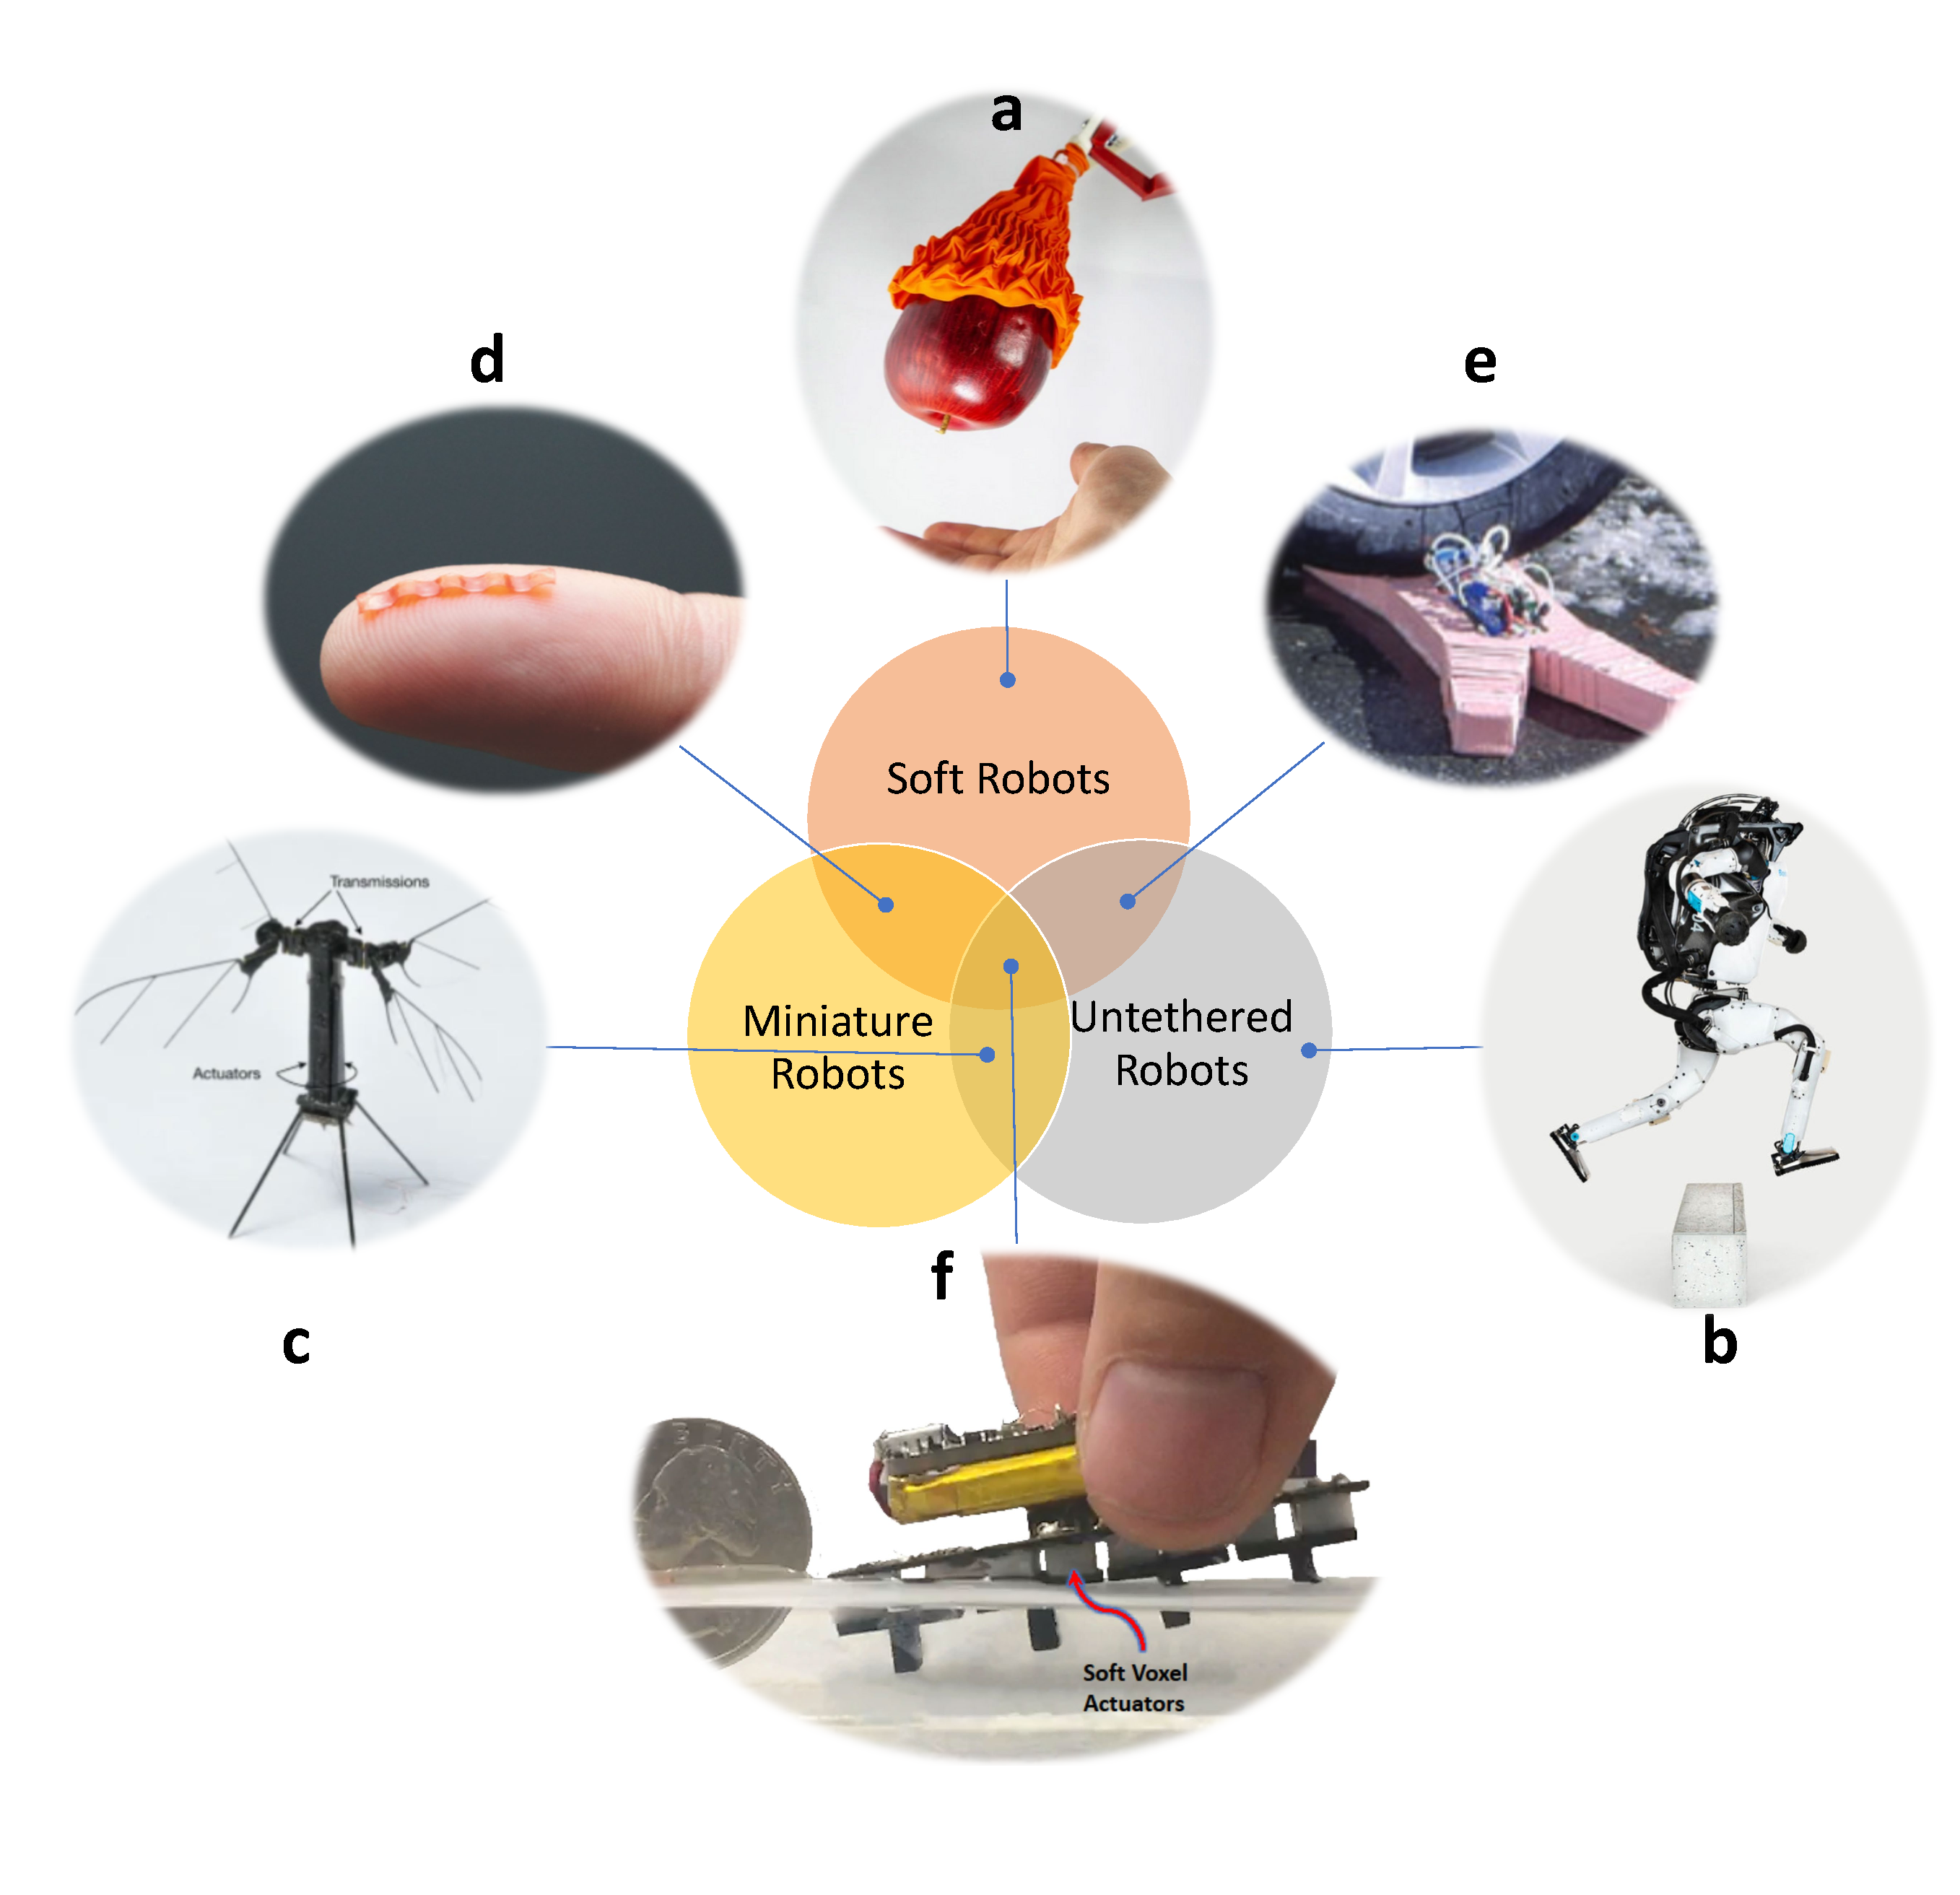
\includegraphics[width=\textwidth]{venn.pdf}
      \caption{Classification of robots. a) soft robot~\cite{Li2019}. b) Untethered robot~\footref{fn:boston} c) Miniature untethered robot~\cite{Jafferis2019} d) Miniature soft robot~\cite{Tingting2012} e) Untethered soft robot~\cite{Tolley2014d} f) Miniature untethered soft robot\textcolor{red}{khodambashi~\cite{}}}
      \label{fig:venn}
\end{figure*}

\section{Soft Robotics as an Emerging Field}
\label{sec:emerging}
Majority of biological organisms contain soft tissue. The soft tissue brings some advantages to these organisms. Octopus is the most widely used source of inspiration for soft robotic research. Octopuses can deform their body and pass through small openings. Therefore, shape morphing is one of the key advantages of soft organisms. Octopuses can also soften their arm as they wrap it around a bottle cap and stiffen their arms for a tight grip as they turn the cap to open it as shown in Fig. Variable stiffness is therefore, another aspect of soft organisms. Human hand is another example which can demonstrate some of the advantages of compliant materials. Human hand can grasp objects with a wide range of shapes and surface roughness without slipping because the soft tissue passively conforms to different shapes (Fig). Human hand can also absorb energy from an impact such as catching a baseball, preventing any damages to the hand. Impact tolerance is another key advantages of soft bodied organisms. The ability to absorb the impact energy also protects the surrounding objects and humans in case of a collision. This brings up safety as another important feature of compliance present in soft bodied animals. The advantages of soft animals are summarized in Table. Inspired by biology, soft robot developers try to utilize the advantages inherent in soft, compliant matter to achieve safer interactions around humans or more robust locomotion and manipulation in unstructured environments~\cite{martinez2013,laschi2012,Tolley2014d,AdamBilodeau2015}.

\section{State of the Art in Soft Robotics}
Traditionally, robots were made to be stationary. They were unaware of their surroundings and operated based on a prescribed set of instructions. Recent advances in sensor technologies have paved the road to mobile autonomous robots which here, are categorized as untethered robots. Therefore, in addition to soft actuators, sensors and computers are also an integral part of any untethered robotic system. For a soft robot, ideally all these components should be soft. Here, the state of the art technology in each category is reviewed with a special attention paid to the soft actuators which is the focus of this dissertation. 
%Soft robots are categorized based on many different features. Here, we focus on miniature and untethered robot categorization to stay focused on the topic of this thesis. Since manufacturing is part of the contribution of this thesis, a brief survey of the manufacturing techniques is also presented.
%\subsection{Components of a Soft Robot}
\subsection{Soft Sensors}
The research on soft sensors focuses mainly on the stretchable sensors for wearable health monitoring~\cite{Liu2017c,Amjadi2016a}. Since these sensors have desirable characteristics, researchers have started to use these sensors in soft robots. Sensors based on liquid metals have particularly been successfully implemented to measure the strain in soft silicon-based devices~\cite{Hammond2014,Chossat2013, Wang2019c,Ren2020}. Other sensor technologies are piezoresistive~\cite{Georgopoulou2020,Turgut2018,Melnykowycz2016}, capacitive~\cite{Hohimer2020,Cao2020,White2017,Frutiger2015}, and conductive polymers~\cite{Chen2021,Kanoun2021,Harito2020}. Majority of these sensors work based on the change in resistance of the material when they undergo strain. 
\subsection{Soft Computers}
Traditionally,  majority of the computations happen on microcontrollers made of hard materials. This is unavoidable and is one of the major limiting factors in the development of entirely soft robots. Soft computers are in their incipient stage. They are based on pneumatic circuits and can perform simple logic functions~\cite{Preston2019,Garrad2019}. Another research direction is using the living cells as computers~\cite{Daniel2013}. This area also needs significant development before it can be successfully implemented in the structure of soft robots. 
\subsection{Soft Actuators}
Actuation is the core of a robot and as such, there is a larger amount of research on soft actuators as compared to soft sensors and computers. Soft pneumatic actuators (SPAs) \cite{Gorissen2017, Branyan2018} are the most widely used category of actuators in soft robotics. They are based on a chamber made of soft materials which is pressurized using fluids. The chamber deforms as a result and produce motions such as bending, elongation or twisting. SPAs have high power to weight ratio and have relatively fast response.  Another class of actuators use active materials that undergo a strain based on a stimulus. This class includes shape memory alloys (SMAs)\cite{Cianchetti2014}, dielectric elastomer actuators (DEAs)~\cite{Carpi2008,Gu2017}, liquid crystal elastomers (LCEs)~\cite{Kularatne2017,Yu2015a}, and stimuli-responsive hydrogels~\cite{Calvert2009,Liu2020,Ionov2014,Banerjee2018}. 
 
%\subsection{Untethere d Soft Robots}
%For functioning as mobile robots, the essential accessories such as pumps or power supplies need to be embedded in the robot itself. These robots fall under the category of untethered soft robots [].  
%\subsection{Miniature Soft Robots}
%Miniature robots have dimensions under...and have a low load carrying capacity. These robots have applications where small loads need to be applied, in working with delicate objects, or in tight environments such as inside human body. 
%\subsection{Miniature Untethered Soft Robots}

%\subsection{Soft Robot Manufacturing Techniques}
%\subsubsection{Molding}
%\subsubsection{3D Printing}
\section{Challenges Ahead}.
Initially, the focus of soft robotics was to find manufacturing methods for SPAs and assemble them into functioning prototypes. These robots were made for tasks such as grasping or used as stationary continuum manipulators. In these applications, the size and weight of the accessories is less important because the accessories are located near the robot and does not have to be carried by the robot. In case of mobile robots however, it is necessary to include all the accessories within the robot and therefore, careful design is required to meet the weight limitations. This challenge becomes more serious in case of miniature robots. SPAs use passive materials such as silicone and rely on rigid components such as motors and pumps that are difficult to downscale and therefore, manufacturing small-scale soft actuators which have applications as envisioned by \cite{hines2017} has remained a bottleneck in the development of miniaturized soft robots \cite{majidi2019}. This category of soft robots are least explored due to complicated materials and fabricating processes. Small-scale actuators can be produced using responsive materials such as DEAs, LCEs and hydrogels. These actuators lack sensing and computation which are essential subsystems of a true robot and are usually used in a human-in-the-loop scenario where sensing and computation are performed by a human operator. This helps in down scaling the robots to the micrometer range. These actuators can perform limited robotic functions and have highly specific applications such as to perform a colon tissue biopsy. However, these robots can not function as autonomous robots because they lack sensing and computation and rely on external devices for their operation. For instance,~\cite{Palagi2016} needs a light projecting device to generate the light patterns required for creating deformations and movement in a light-responsive actuator. Another example is a magnetic-responsive actuator~\cite{Kim2018} which rely on a magnetic field generator for its operation. All these equipment are bulky and require careful setup and therefore, these types of actuators are not suitable for use in autonomous mobile robots. Technologies are still needed to create small-scale autonomous soft robots that function similar to biological organisms such as annelids, mollusks, and octopuses. Considering the highly sophisticated structure of living organisms, simultaneous progress in multiple disciplines such as materials science, design, manufacturing and control is required in order to achieve soft robots that are closer to their biological counterparts.

Hydrogels are close to soft tissue in terms of material properties and the muscle like contractions in response to external stimuli~\cite{Liu2020}. Also, they can be made to be ion conductive and biocompatible. These features can add up to the benefits of soft robots namely safety and adaptability~\cite{Lee2020}. However, the uniform responsive volume change of bulk hydrogels makes it less interesting in robotic applications, which instead demands complex spatiotemporal reconfigurability~\cite{Erol2019} - as the dexterous octopus arm presents. The challenge is to create 1) on-demand, 2) time-varying and 3) local deformations in a hydrogel structure. From a structural design perspective, the majority of reported heterogeneous hydrogel structures demonstrate fixed deformation patterns, such as static shape shifting of sheets without any interaction with the environment~\cite{SydneyGladman2016, Ma2019, Jeon2017} or bending of beams to perform simple gripping functions ~\cite{Wang2017, Ma2018, Duan2017} Only a few methods demonstrate on-demand deformations and are able to interact with objects~\cite{Mourran2017, Palagi2016, Kim2018} but involve bulky equipment (light and magnetic field generators), making them impractical for mobile soft robots or embedded applications.
From a materials perspective, there is a need for a powerful but simple synthesis method to broadly tune the material response behavior (volume changing ratio, speed, and stiffness), to meet the requirement of creating a complex robotic structure with spatiotemporal reconfigurability.

\section{Contributions of this Dissertation}
This dissertation demonstrates progress in different areas of material science and manufacturing  that together, will contribute to the field of soft robotics. A set of design decisions are made based on closed collaboration of teams of material scientists and roboticists which helps the informed progress of one field by considering the requirements of the other. A bioinspired approach is used to help with some of the design decisions. Biological organisms use electrical signals from the nervous system in conjunction with responsive muscle tissue to perform soft actuation. This combination helps them to be self-contained and also, it is viable across scales from giant octopuses to millimeter-sized worms. Therefore, the first feature that is considered for the design of soft robots is to use a material that is responsive to electrical stimulus. The living organisms also are made of cells which are simpler building blocks assembled to form a more complex organ. The second requirement imposed is therefore, to use a bottom-up strategy to fabricate complex robots using simple building blocks that are easy to manufacture. The contribution of this dissertation as shown in Figure~\ref{fig:summary} can be summarized as follows:

\begin{itemize}
	\item A novel, temperature-responsive hydrogel material with fast response. This material functions as artificial muscle tissue. 
	\item A Facile and tunable synthesis method. This makes the synthesis method simple and accessible by the soft robotics community which have less access to material processing facilities.
	\item A voxel-based assembly approach. This helps to use simple building blocks called soft voxel actuators (SVAs) to assemble more complex soft robots. SVAs are easy to manufacture and solve some of the challenges associated with embedding electronics in soft robots.
	\item Electrical Joule heating of SVAs. This enables the use of small footprint microcontrollers and paves the road to embedded and mobile robot applications.
	\item Realization a hyper-redundant hydrogel-based electrically addressable miniature soft robots capable of performing tasks that require high number of DOF. High dexterity and the ability to function in unstructured environments are functionalities, which separates our devices from previously demonstrated structures.
	\item Realization of a miniature untethered soft robots. This robot weighs only 20g including battery and power supply and does not rely on external equipment or human intervention for its operation.
\end{itemize}
\begin{figure*}[!ht]
      \centering
      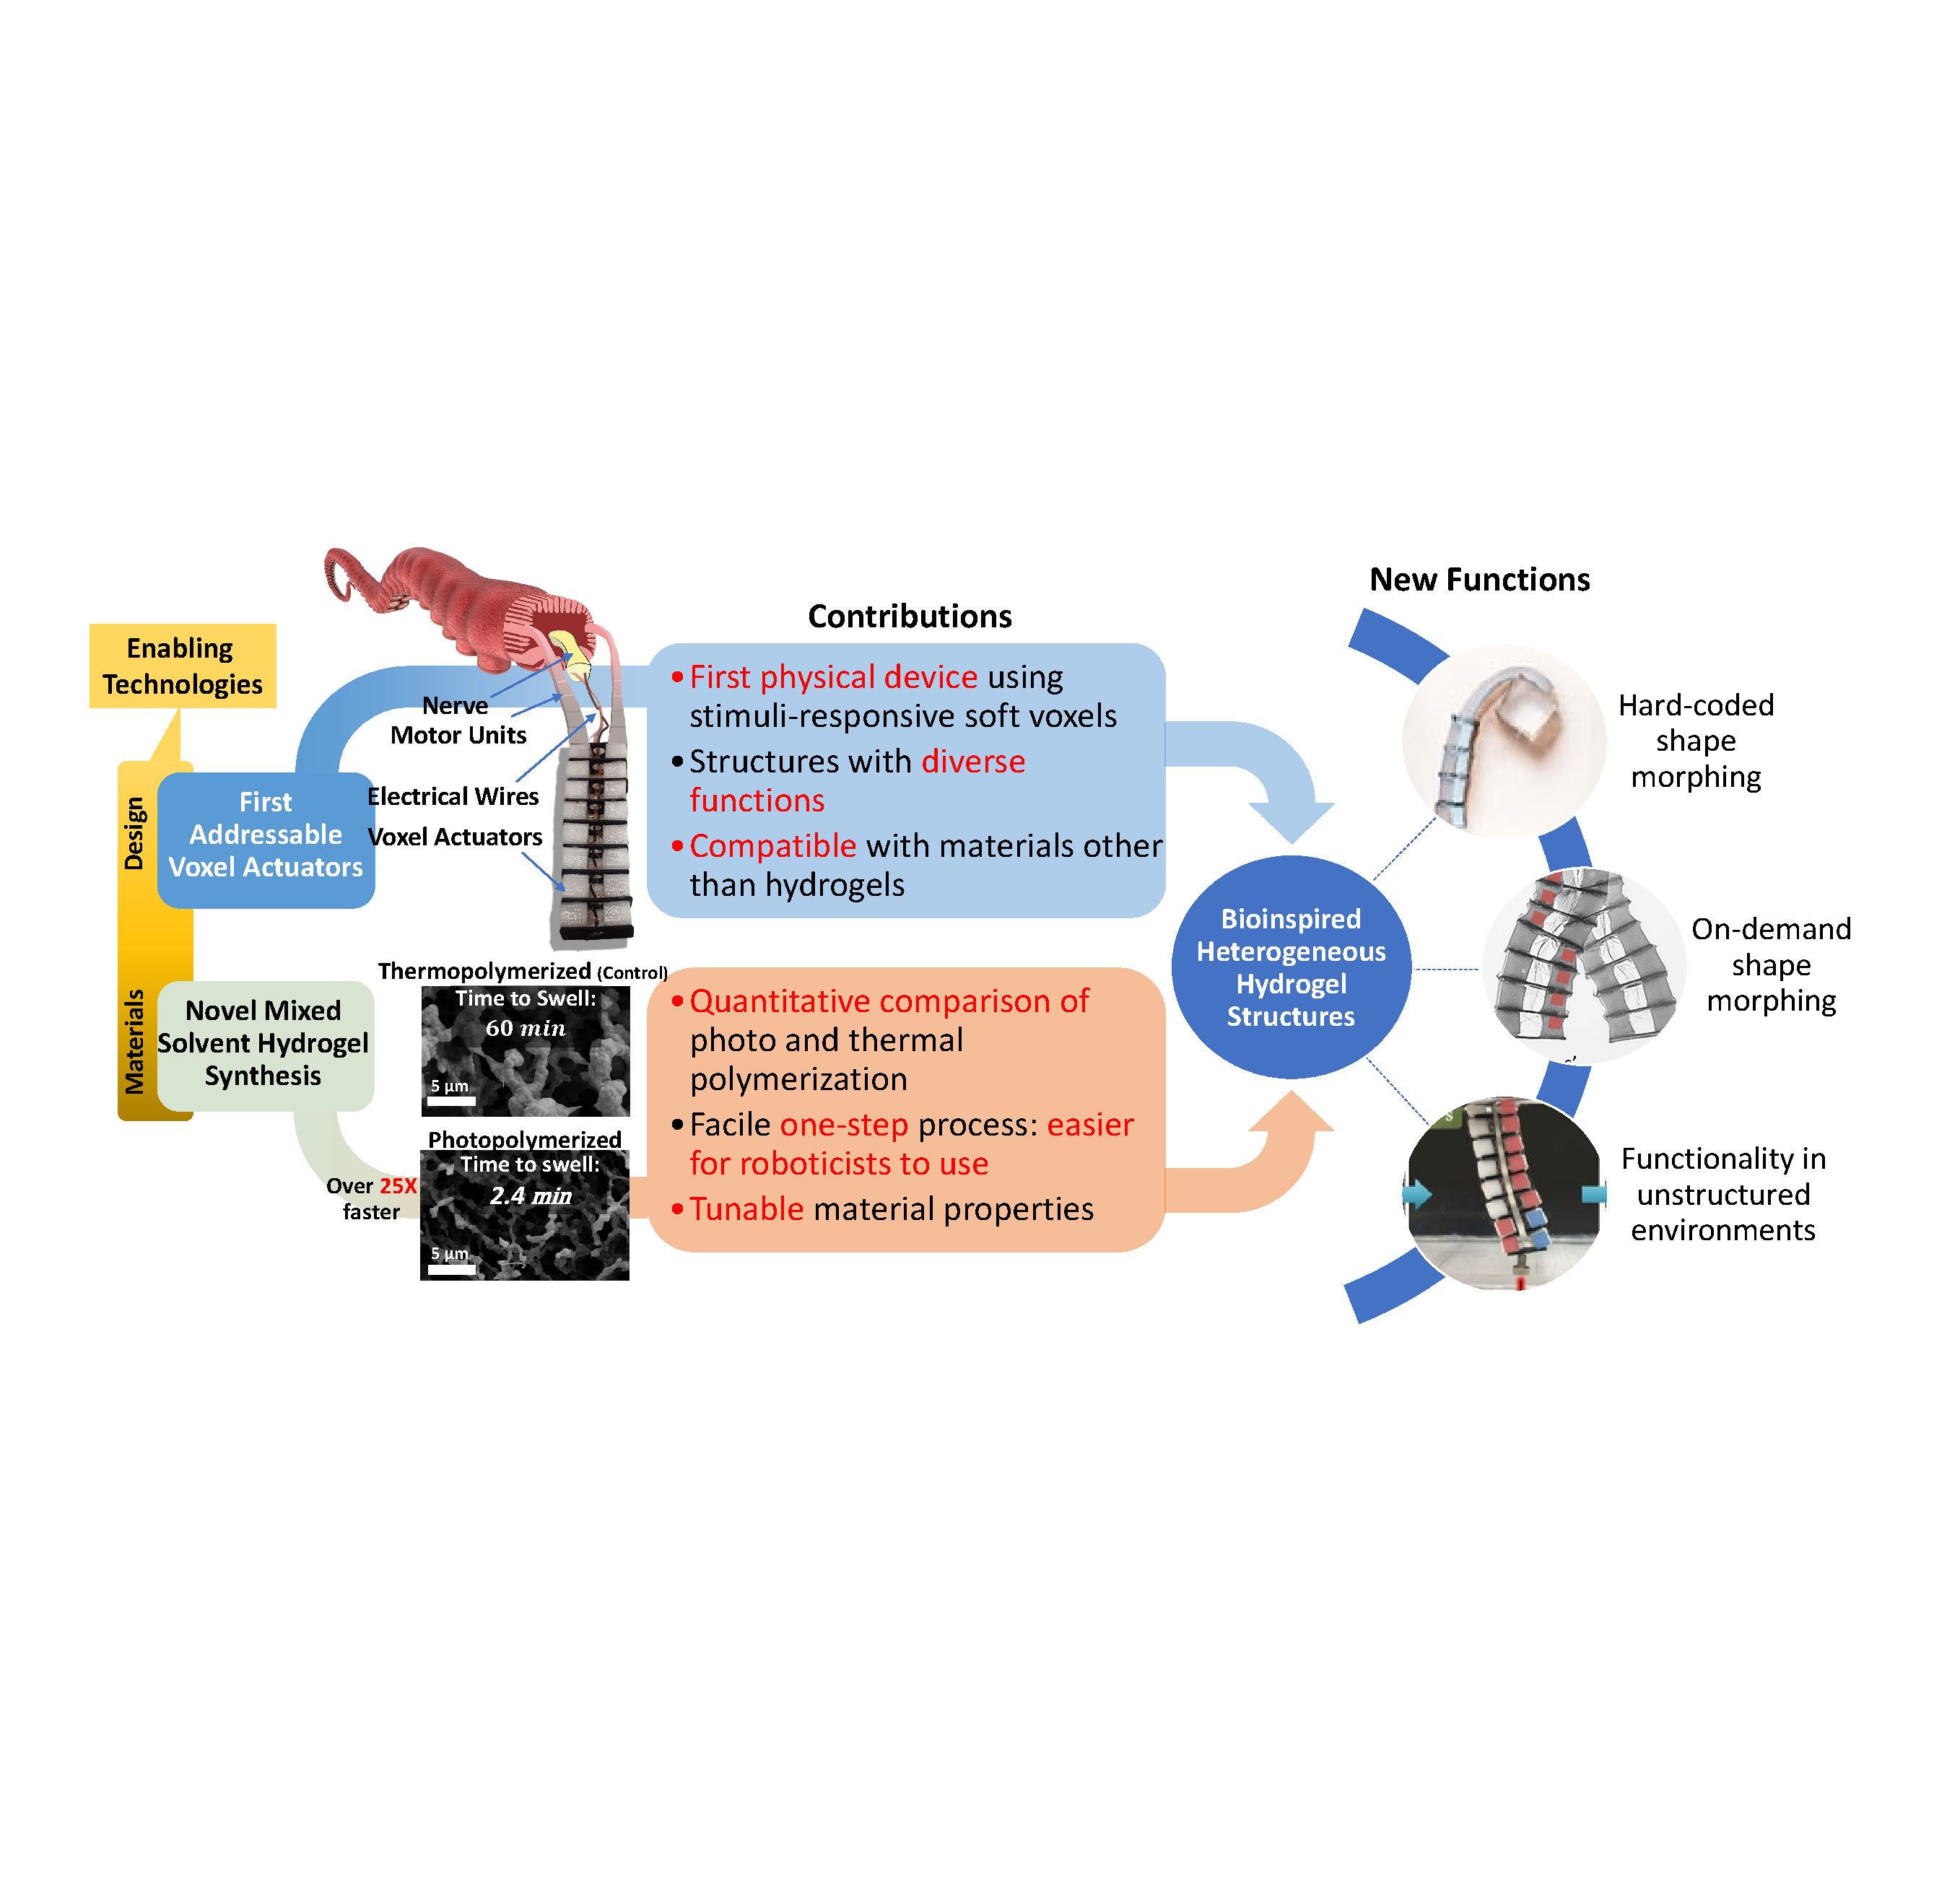
\includegraphics[width=\textwidth]{summary.pdf}
      \caption{Classification of robots. a) soft robot~\cite{Li2019}. b) Untethered robot~\footref{fn:boston} c) Miniature untethered robot~\cite{Jafferis2019} d) Miniature soft robot~\cite{Tingting2012} e) Untethered soft robot~\cite{Tolley2014d} f) Miniature untethered soft robot\textcolor{red}{khodambashi~\cite{}}}
      \label{fig:summary}
\end{figure*}
%\subsection{Broader Impact}
%\subsubsection{Scientific}
%Current soft actuators rely on additional hardware such as pumps, high voltage supplies, light generation sources and magnetic field generators for their operation. These components resist miniaturization and embedding them into small-scale soft robots would be challenging. This limits their mobile applications especially in hyper-redundant robots where a high number of actuators are needed. On the other hand, our developed SVAs weigh only 100 mg and require small footprint microcontrollers for their operation which can be embedded in the robotic system. 
%\subsubsection{Social}
%Soft robots are intrinsically safe around humans. This can help bring robots to daily life applications such as household robots and assistant robots for elderly people. Also, our soft robots can operate underwater due to hydrogel compatibility with moist environments. A swarm of soft robots can be used for underwater exploration and data collection and help monitor the climate change through recording the water current temperatures over long period of time.

\subsection{Dissertation Outline}
The following chapters discuss the innovations in materials science and manufacturing methods that lead to the development of miniature untethered soft robots.\\ 
\textbf{Chapter~\ref{chap:SVAs}: Soft Voxel Actuators: Hydrogel Building Blocks for Bottom-up Assembly of Soft Robots}\\
This chapter discusses the recipe for preparing temperature-responisve hydrogels. Improvements have been made in the synthesis technique such that it is more accessible to robotic researchers who have less access to material processing facilities. In addition, this recipe results in hydrogels with fast response, solving a challenge that has limited the use of hydrogels in soft robotics. Next, building blocks called soft voxel actuators (SVAs) are introduced that facilitate the manufacturing of soft robots through a bottom up assembly approach. Both the hydrogel and SVAs are characterized in-depth in terms of material properties and actuation properties.
  
\textbf{Chapter~\ref{chap:heterogeneous}: Heterogeneous hydrogel structures as Miniature Hyper-redundant Soft Manipulators}\\
This chapter is case study I of the application of SVAs and is focused around miniaturizing soft robots without loosing their functionality as a result of reducing the number of degrees of freedom. Hyper-redundant miniature soft robotic manipulators are developed. It is shown that the use of SVAs facilitates the development of such robots. These robots are able to work in unstructured environments where the working conditions might change. This manipulator has 16 actuators in a ... footprint which is the highest reported number of degrees of freedom in a miniature robot of this dimension.

\textbf{Chapter~\ref{chap:untetheredWalker}: Miniature Untethered Underwater Walking Robot}\\
This chapter is case study II of the application of SVAs and is focused around the development of untethered miniature robots. It is demonstrated that the use of SVAs can significantly reduce the weight and size of the robots. These robots are fully untethered which means all the electronics and the power source is included in the robot. 

\textbf{Appendix~\ref{chap:control}: Tracking Control of a Miniature 2-DOF Manipulator with Hydrogel Actuators}
The electrical stimulation of SVAs inspired by biology has many advantages and open the doors to equip the robots with artificial intelligence. As a first step, the automatic control of the SVAs using a microcontroller is presented in this chapter. Instead of turning the SVAs on and off as explained in Chapter~\ref{chap:heterogeneous}, the deformation of SVAs are controlled using a closed-loop control system based on the feedback from vision sensors which record the desired output of the system. A 2-DOF manipulator is fabricated using two SVAs and the position of the tip of the manipulator is controlled. As the final demonstration, a starfish inspired robot is presented which can carry a payload. The closed-loop control helps the payload transport to reach a higher speed compared to an open loop control. 


\graphicspath{{Images/SVAs/}}

\chapter{SOFT VOXEL ACTUATORS: HYDROGEL BUILDING BLOCKS FOR BOTTOM UP ASSEMBLY OF SOFT ROBOTS}
\label{chap:SVAs}
Soft continuum manipulators are suitable for safe interaction with unstructured environments due to their compliance and theoretically infinite degrees of freedom (DOF). However, since current soft actuators resist miniaturization, using a large number of them to activate each DOF in a minaturized soft continuum manipulator has remained a challenge. This results in primitive miniature manipulators which have limited functionality. Here, we use a bottom-up voxel-based design and manufacturing methodology to integrate more actuators in soft robot manipulators while maintaining the small footprint of resulting robots. To solve challenges with miniturizing soft actuators, we introduce soft voxel actuators (SVAs) -- an active voxel actuated by electrical stimulus -- that resembles a group of muscle fibers (fascicles) in size, force production capacity and type of activation stimulus. We report the manufacturing method of SVAs, their frequency bandwith, and their static and dynamic force production capacity. We then show the advantages of the voxel-based methodology by assembling 4.5$\times$ 4.5$\times$4.5\,mm$^3$ SVAs weighing only 100\,mg into a miniature soft, continuum robotic manipulator with 16 DOFs in a 10$\times$40$\times$4.5\,mm$^3$ footprint. The arrangement of SVAs in this manipulator is inspired by the the arrangement of muscle fascicles in an octopus arm. We demonstrate the superiority of the SVA-based manipulator over conventional manipulators in interacting with unstructured environment. 
\section{Background}
\begin{figure*}[t]
      \centering
      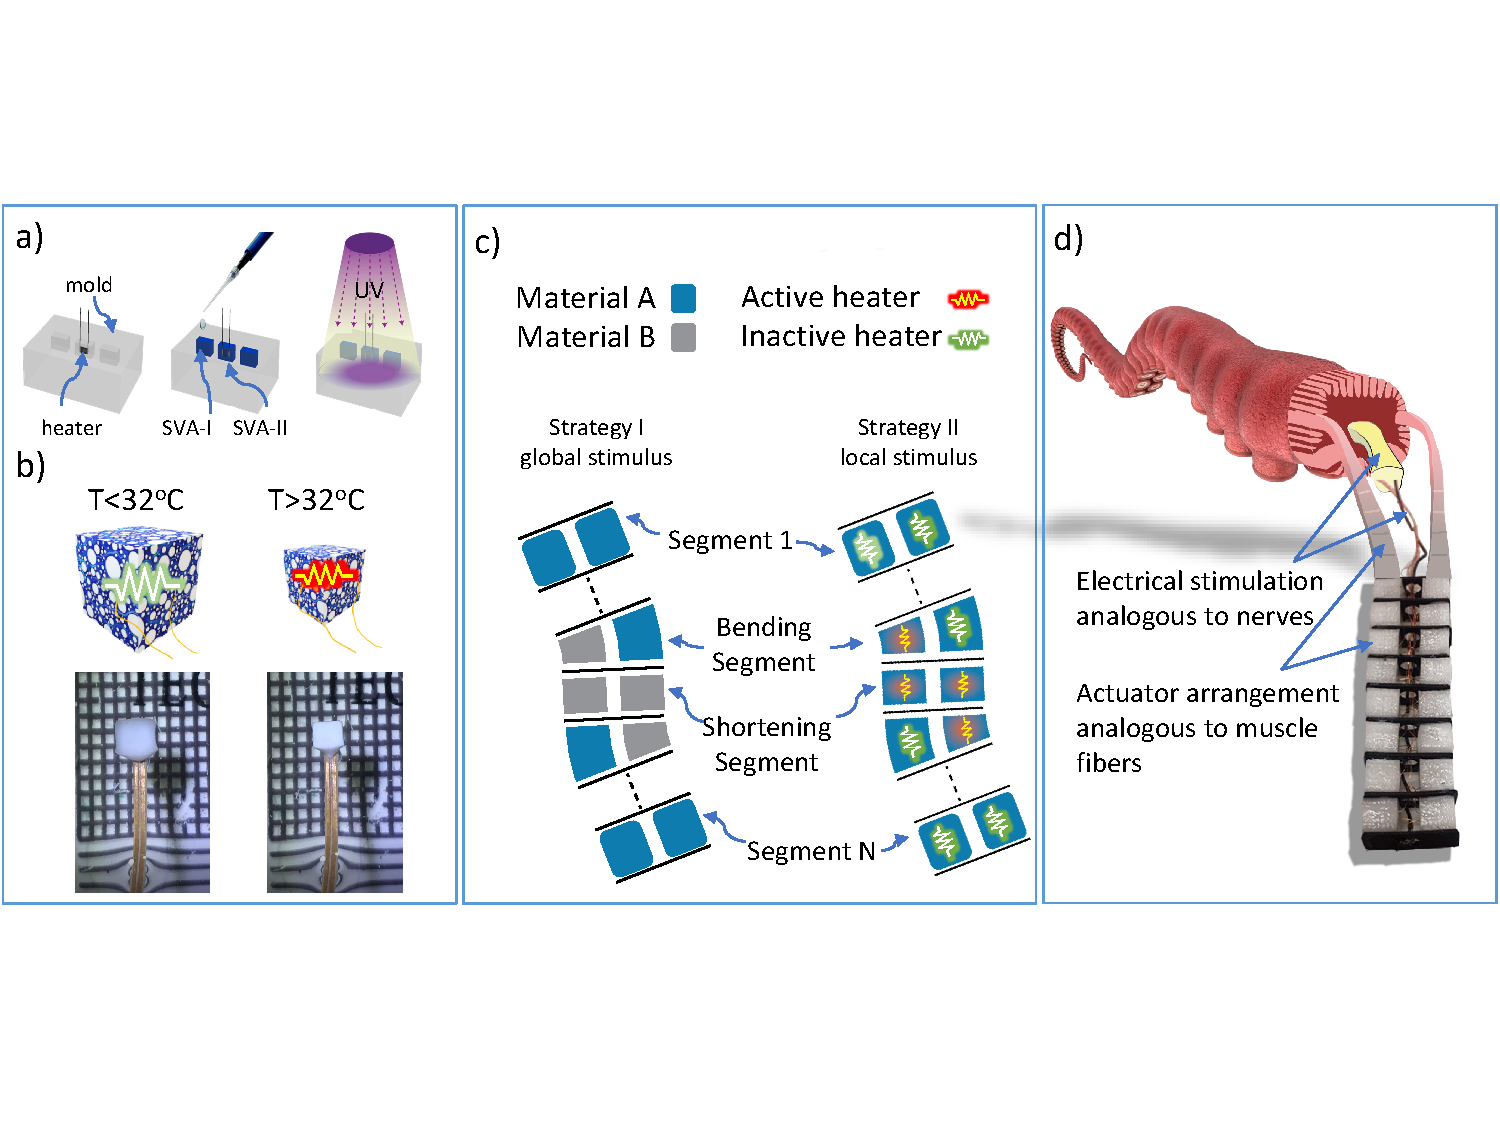
\includegraphics[width=\textwidth]{concept4.pdf}
      \caption{A: SVA manufacturing steps, B: a SVA in its actuated and unactuated staes C: The voxel-base design and manufacturing methodology based on electrically addressable SVAs has made possible the creation of miniature continuum manipulator with 16 DOFs.}
      \label{fig:conceptSVA}
\end{figure*}
Inspired by biology, soft robot developers try to utilize the advantages inherent in soft, compliant matter to achieve safer interaction with unstructured environments.  
While the applications of small-scale soft robots have been demonstrated or envisioned by many research groups \cite{hines2017soft}, miniature and micro-scale soft robots have matured more slowly than their  macro-scale counterparts. The majority of soft robots utilize rigid components such as motors and pumps that are difficult to downscale \cite{majidi2019soft} and therefore, manufacturing small-scale soft actuators has remained a bottleneck in the development of miniaturized soft robots. Smart, soft materials have shown promise in solving some of these challenges \cite{steele2018stimuli, stuart2010emerging,white2013advances}; these smart materials react to changes in pH, temperature, or electric, magnetic and light fields by producing stress/strain fields in the material to create motions such as bending, twisting, or elongation. These motions have been harnessed for applications such as drug delivery \cite{ghosh2017stimuli}, micro-grippers \cite{shintake2018soft}, or other primitive robots~\cite{ionov2014hydrogel}. %such as dielectric elastomer actuators (DEAs), ionic polymer-metal composites (IPMCs) and stimuli-responsive hydrogels 
%Performing sophisticated tasks while interacting with unstructured environments requires independent actuation of many degrees of freedom in coordination with each other. Smart soft materials have nearly infinite active degrees of freedom meaning each infinitesimal region can be considered as a virtual actuator. The nature of stimuli such as PH, magnetic fields or electric fields however, prevents systems of actuators from being individually addressed. As a result, these materials are often activated globally, meaning that all the virtual actuators in the material are activated at the same time using a stimulus that acts globally on the entire system \cite{ceylan2017mobile}. Structured light has been shown to address this issue by independently addressing more degrees of freedom in smart soft materials \cite{palagi2016structured}. This method, however has other limitations, as the light cannot reach the interior of material volumes to excite regions that are out of sight. The most intuitive and bio-inspired stimulation technique is electrical stimulation, which is closest to electrical potentials used in the nervous systems of living animals. Common materials that can be activated by electrical potentials or currents include DEAs, LCEs and IPMCs\cite{carpi2011dielectric}. Due to the complexity of manufacturing these material systems, miniature robotic mechanisms in the literature that use these materials [] have demonstrated only a few degrees of freedom. Utilizing higher number of virtual actuators inherent in these materials can become challenging. DEAs, for example, require high voltages which in turn requires additional, often bulky electric components; IPMCs produce only bending motions and exhibit other non-ideal behaviors such as Back Relaxation \cite{annabestani2016restraining}. Robots resulting from these materials have remained primitive in the sense that they can only perform simple, context-specific tasks that they are designed for. When the task changes during their operation-- a case which often happens in unstructured environments-- these robots fail.  
%
%
%Temperature responsive hydrogels, by contrast, can be stimulated electrically using Joule heating \cite{yu2013electronically}. The electrical stimulation can be confined to micron-sized regions making it possible to individually address more virtual actuators in the material \cite{richter2009optoelectrothermic}. However, they are usually sluggish in their response especially at larger scales, making them unsuitable for many robotic applications. We have previously reported solving the problem of slow response of temperature responsive hydrogels \cite{emami2019}. Based on that result, we now present a novel, soft actuator along with a design methodology for solving some of the challenges related to miniaturizing soft actuators and the resulting soft robots. These actuators, which we called soft voxel actuators (SVAs), are made using temperature-responsive hydrogels and electrically activated by Joule heaters. Our design and manufacturing approach is to consider the entire body of a soft robot as a collection of smaller units called voxels. %ach SVA is the physical realization of the virtual actuators inherent in smart soft materials.
%Assembly of these voxels results in a soft robot with many individually addressable degrees of freedom. %Since each voxels is an individually-addressable actuator, the resulting robot contains many degrees of freedom that can be controlled electrically. %In addition to material properties of tmeperature-responsive hydrogel used in OUR SVAs, the performance of the actuators is also dependent on the shape, and working conditions of the actuator. Therefore, in this paper, 
%We have characterized the force and stroke of each SVA and proposed bio-inspired configurations (Figure~\ref{fig:conceptSVA}) for assembling SVAs in ways that results in general miniaturized mechanisms capable of performing more sophisticated tasks than found in current literature. We can demonstrate that SVAs can be used in a bottom-up approach to build miniature continuum manipulators with hyper-redundant DOFs. This miniature manipulator is 10$\times$ 40 $\times$ 4.5\,mm$^3$ and has 16 DOF making it robust in creating complex interactions with unstructured environments.  
%\textcolor{red}{This paper demonstrates how SVAs support the development of soft, miniature continuum, robotic arms  -- a challenge difficult to realize with competing technologies}.
%
%\section{Soft Voxel Actuators (SVAs)}
%In computer-based modeling or graphic simulation, the word ``voxel'' typically refers to 3-dimensional (3-D) units used to represent shapes in 3-D space; they are the 3-D equivalent to pixels, which are used for representing objects and images in 2-D  space \cite{sossou2019design}. The recent use of physical voxels in additive manufacturing, using passive and often rigid materials,  has been demonstrated in literature and patents \cite{hiller2009design}. However, the physical realization of soft voxels using stimuli-responisve materials that can act as individually-addressable actuators has not yet been demonstrated. Manufacturing and characterization of such actuators as simple building blocks for use in a bottom-up approach to construct complex robotic systems is demonstrated herein.
%
\subsection{SVA Fabrication}
SVAs were made through a molding process in the form of cubes of different dimensions, as shown in Figure~\ref{fig:Manufac}. The molds were made with PDMS (Sylgard 184, Dow Corning) because of its transparency to UV light and its elasticity, so that the cured hydrogel may be easily and fully demolded without breaking. Since the hydrogel swells from its molded dimensions upon soaking in water, the dimensions of the molds were selected to be smaller than the required dimensions of the actuator. A nylon mold was prepared using a 3D printer (Markforged, M2) and was used to create the PDMS mold. For selecting Joule heaters, several types of resistive heaters were examined to find the optimum one in terms of manufacturability, durability, and compatibility with other electronic components. Surface mount resistors have all the required properties and therefore were chosen as the heating elements (Figure~\ref{fig:Manufac}). The value of the resistor was chosen such that it produced enough heat to set the equilibrium temperature of the SVA from room temperature ($25^{o}C$) to above the transition temperature of the hydrogel ($32^{o}C$) and cause it to shrink when a 3.7 $V$ supply voltage was connected to it. This actuation voltage was chosen to be compatible with many commonly used microcontrollers that are available on the market. In this paper, we have used surface mount 
(SMD) thick film resistors with a resistance of 10~ohms which is shown in Figure~\ref{fig:Manufac} along with its dimensions.  For manufacturing each SVA, a resistor (Joule heater) was positioned inside the mold using an XYZ manual stage (Figure~\ref{fig:Manufac}) before the precursor solution was added and cured along with the gel. The heater was placed at a position equidistant from each side of the mold so that the entire volume of the gel was heated as uniformly as possible to avoid undesired nonuniform deformation of the actuators. PNIPAAm precursor solution was poured into the molds using pipettes while the resistive heater was held in place using grippers. A UV LED (UV 365nm, 10W, Chanzon, China) was used for curing the gels. 

\begin{figure*}[h]
      \centering
      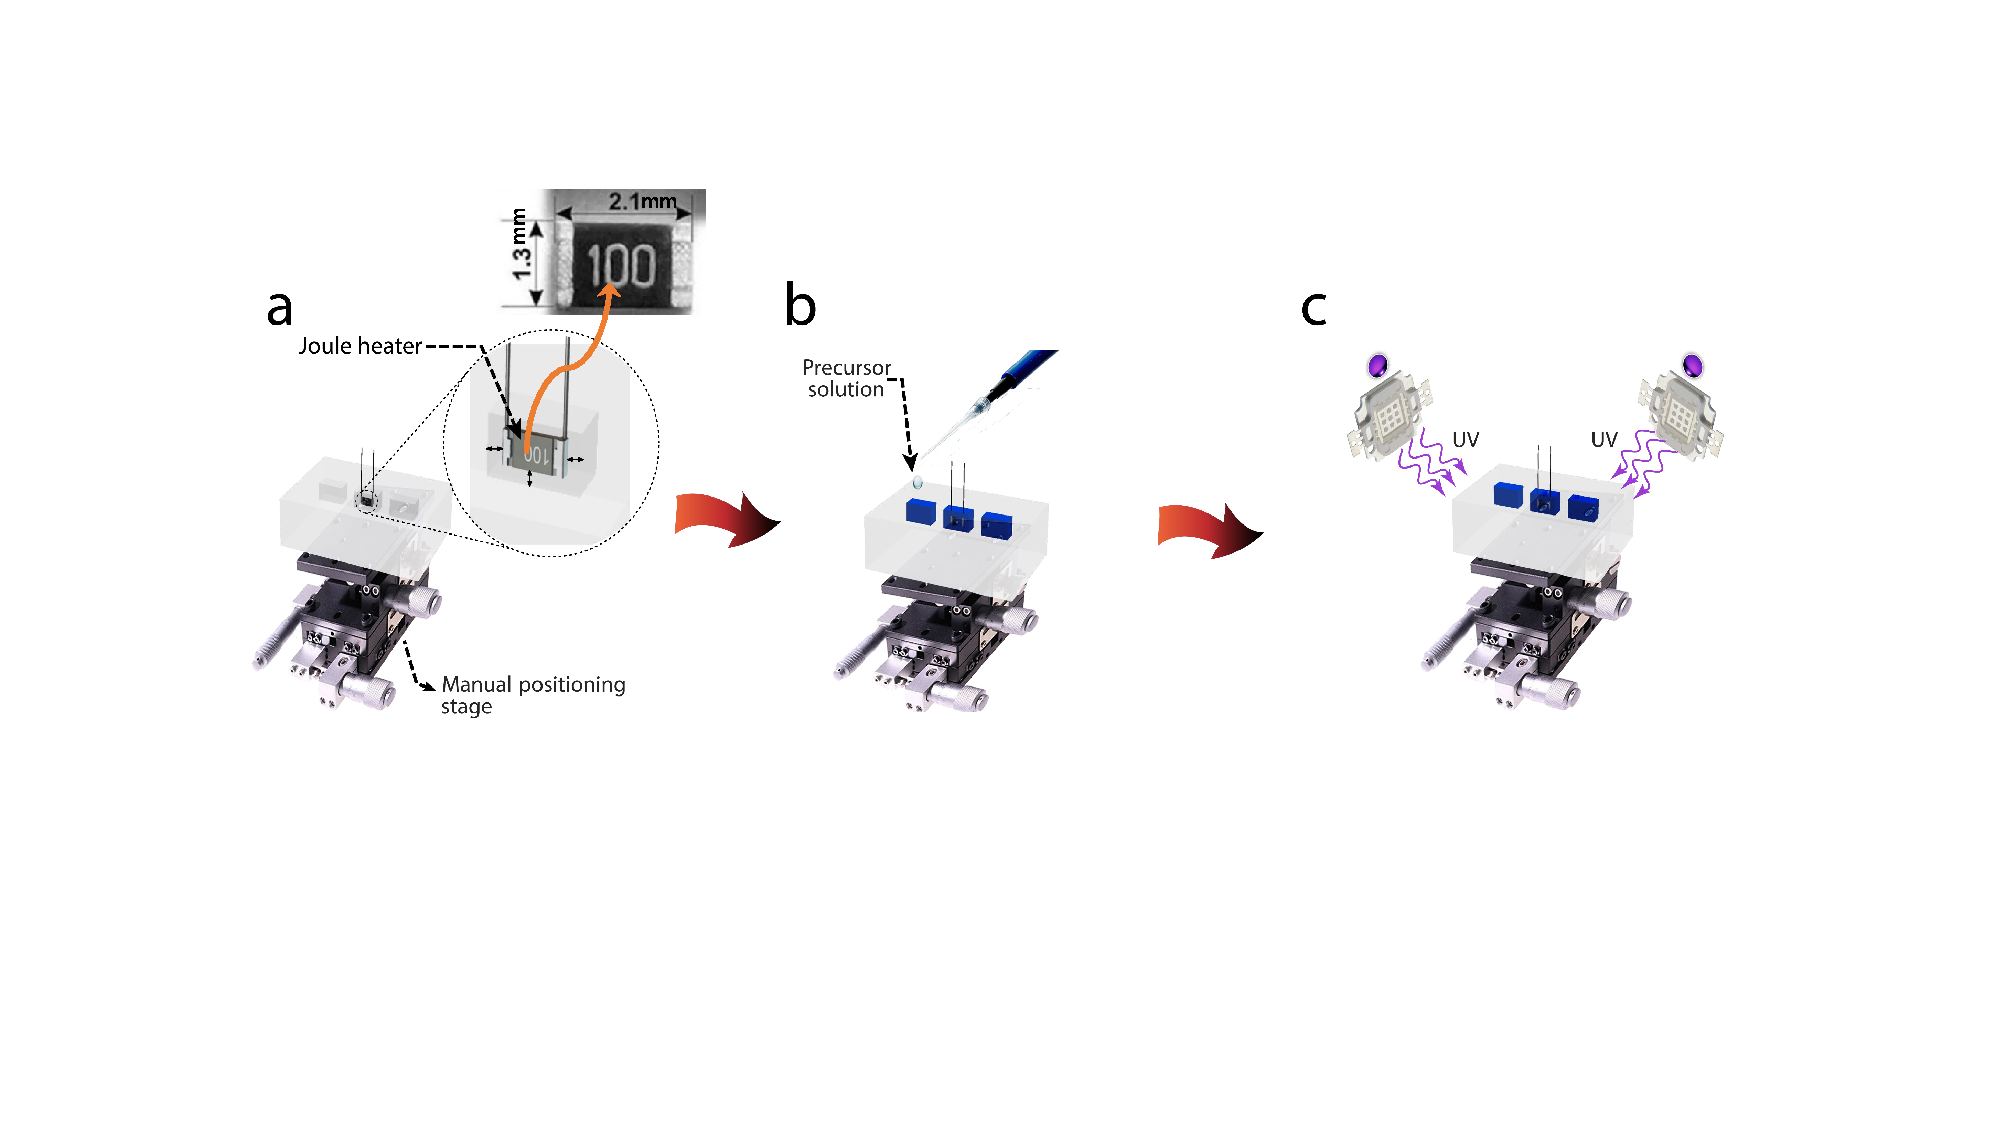
\includegraphics[width=\textwidth]{svaManufacturing.pdf}
      \caption{Steps for manufacturing SVAs. A) A Joule heater (surface mount (SMD) thick film resistors with a resistance of 10 ohms) is placed in the PDMS mold using an XYZ manual stage. B) Precursor solution is added to the mold. C) Hydrogel is formed by curing the solution under UV light for 10 seconds.}
      \label{fig:Manufac}
\end{figure*}

\subsection{SVA force measurements}
The force generated by an SVA was measured using a 100~g load cell and a load cell bridge amplifier (PhidgetBridge 1046_0B, Phidget, Canada) in the setup shown in Figure~\ref{fig:forceTestSetup}. The SVA was placed under the load cell, the joule heater was activated allowing the SVA to shrink to its minimum volume, and then the linear stage was lowered to bring the load cell in contact with the surface of the SVA as shown in Figure~\ref{fig:forceProcedure}. The interface between the load cell and the SVA was made from an acrylic plate. In force measurement tests where the SVA expands and pushes against the load cell, this plate just touches the surface of the SVA. In other tests where the SVA contracts, superglue was used to bind the acrylic plate to the SVA, so that the SVA pulled on the load cell as it contracted. The experiment is performed in a water bath at room temperature (25$^o$C). The load cell was calibrated while the acrylic plate was underwater but not touching the SVA. A two-point calibration method was used with a 50~g precision weight.

\begin{figure*}[h]
      \centering
      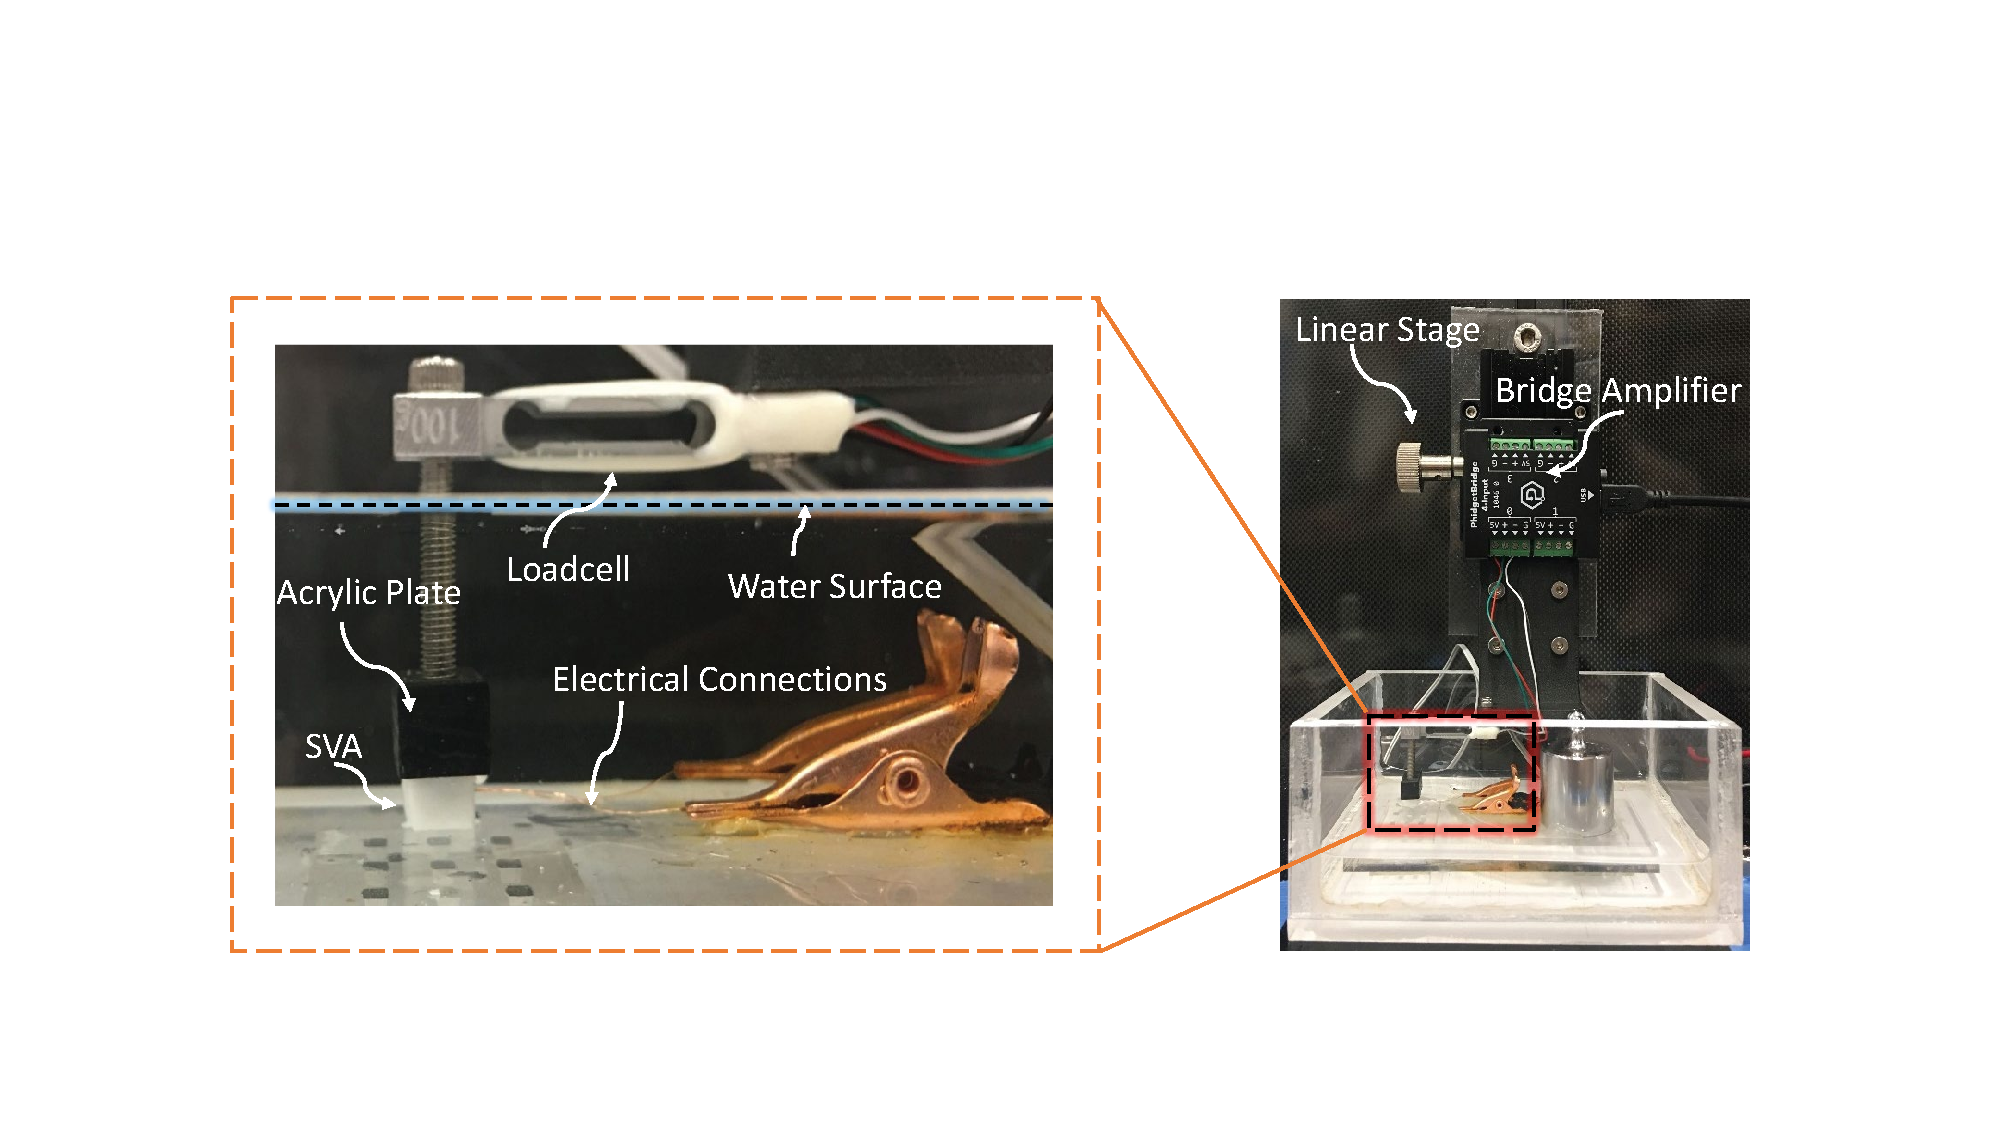
\includegraphics[width=\textwidth]{forceTestSetup.pdf}
      \caption{Steps of placing the sensor tip on the SVA for compressive force measurement.}
      \label{fig:forceTestSetup}
\end{figure*}

\begin{figure*}[!h]
      \centering
      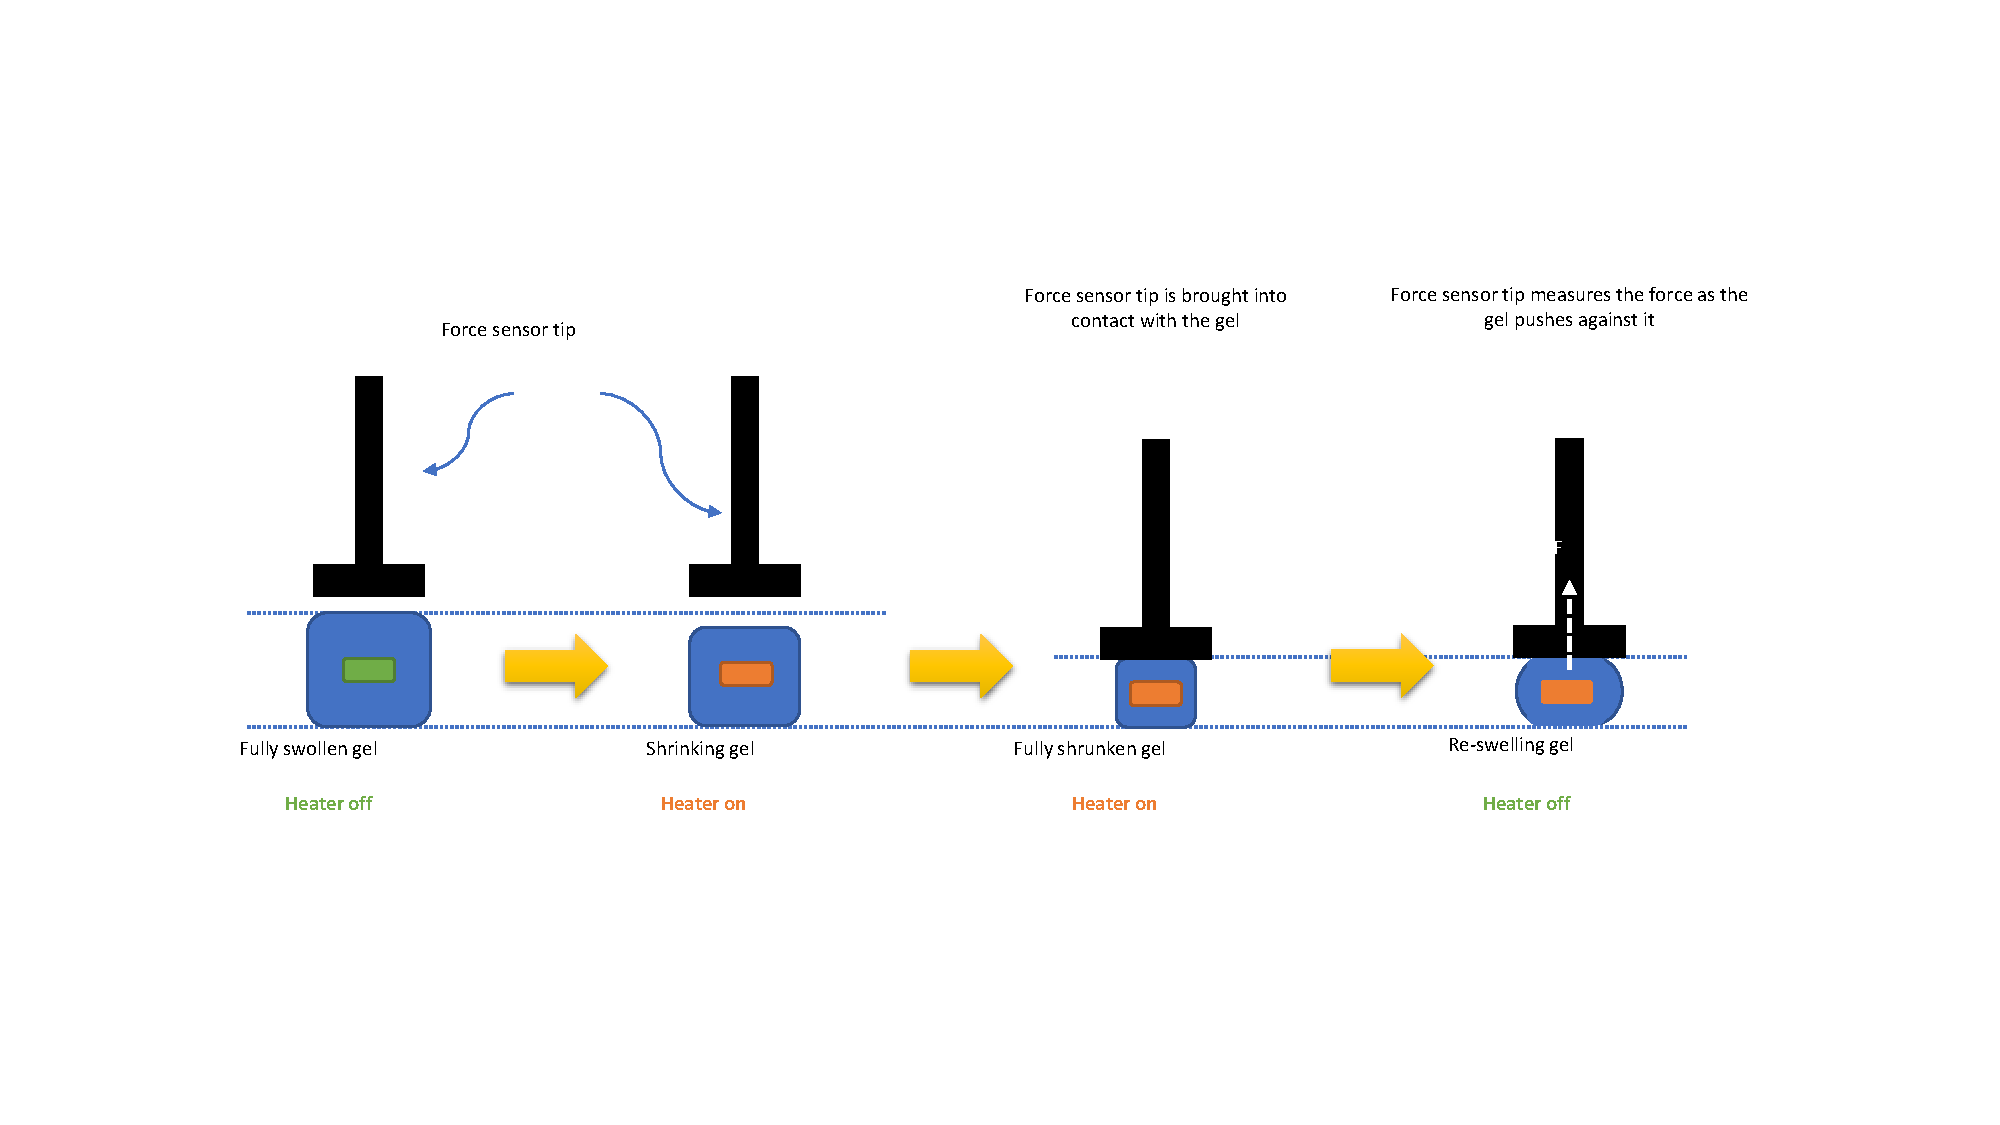
\includegraphics[width=\textwidth]{forceProcedure.pdf}
      \caption{SVA force measurement setup using a load cell and a bridge amplifier.}
      \label{fig:forceProcedure}
\end{figure*}

the force produce by the SVA is depended on its material properties. Since the material properties of the hydrogels can be tuned by varying Figure~\ref{fig:svaForce}
\begin{figure}[!htb]
\centering
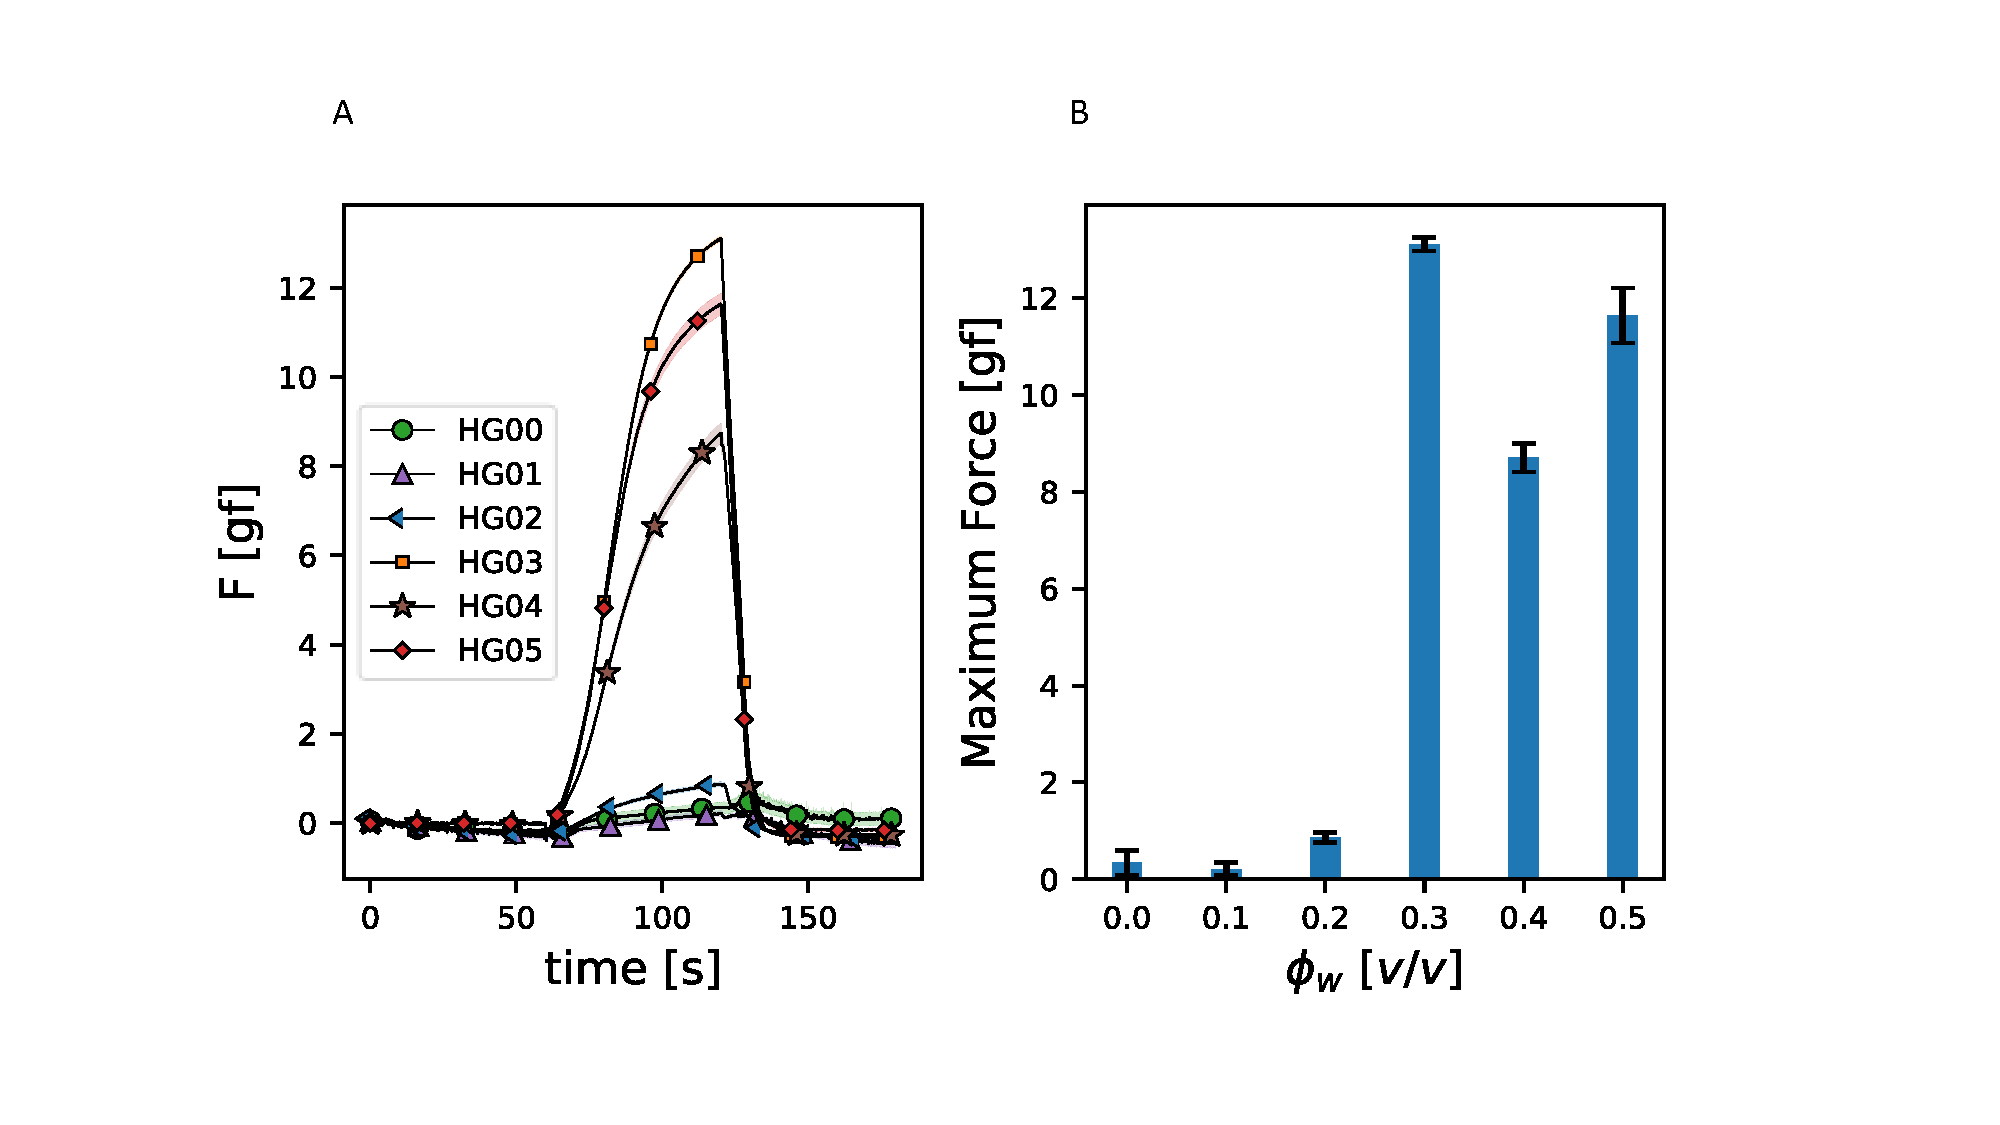
\includegraphics[width=\textwidth]{svaForce.pdf}
    \caption{Tuning the mechanical properties of SVAs by varying water volume fractions $\phi_{w}$. A) Force produced by a SVA as a function of time for different $\phi_{w}$. B) Maximum force produced by a SVA as a function of $\phi_{w}$. }
    \label{fig:svaForce}
\end{figure}

\subsection{SVA swelling ratio measurements}
Swelling ratio, a commonly studied property of hydrogels, is a measure of the ability of the gel to absorb water. Robotics applications which use fast responding hydrogels such as the one presented in this paper require a method of characterization of the hydrogel swelling ratio, to quantify volume changes in real-time in order to capture the volume changes that happen in short amount of time. We have developed a method that uses image processing techniques to measure the linear displacement produced by a SVA, as shown in Figure~\ref{fig:swellingTestSetup} S3. The volume change of a SVA results in the movement of a lever arm contacting the SVA, and the resulting vertical displacement of the tip of the lever arm is then measured. 

\begin{figure*}[!h]
      \centering
      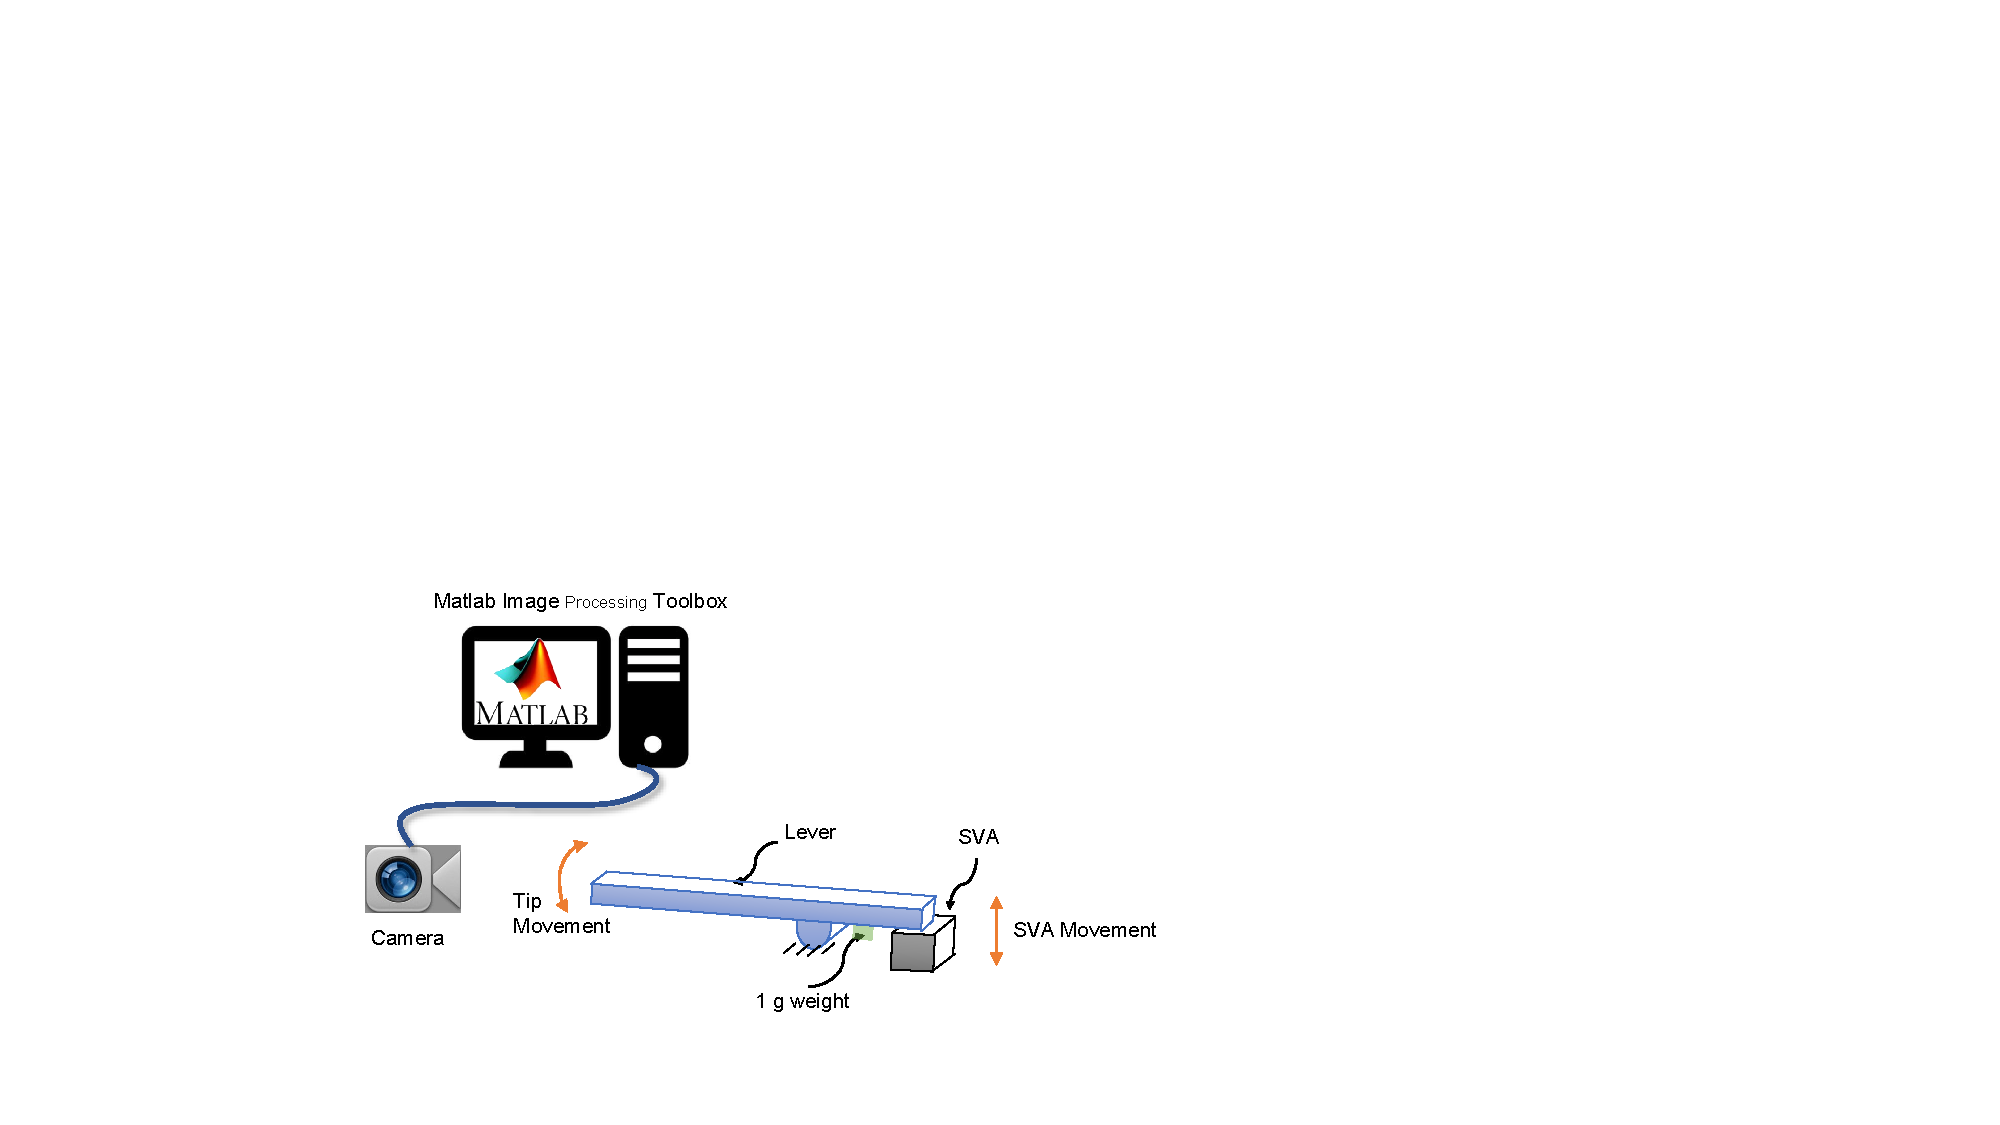
\includegraphics[width=\textwidth]{swellingTestSetup.pdf}
      \caption{SVA displacement measurement setup. A camera is used to track the angular displacement of the tip of a lever arm, which is proportional to the vertical displacement of the SVA (assuming small displacements). The 1 g weight is affixed to the lever arm to ensure that the lever is always in contact with the SVA.}
      \label{fig:swellingTestSetup}
\end{figure*}

Since this vertical displacement is small, the curve followed by the tip can be approximated by a straight line and is proportional to the vertical displacement of the SVA. A marker on the tip is tracked by a Logitech C930e USB Webcam, which can stream HD 1080P quality video. This webcam is compatible with the MATLAB Image Acquisition and Image Processing Toolboxes. In each test, a checkerboard was placed in the same plane as the marker on the tips of the lever arm. This checkerboard had black and white squares of dimensions 2 mm × 2 mm and was used to estimate the calibration factors (mm/pixel) in the x and y directions. Since we used contrast-based filtering, the marker color was selected to be white whereas the color of the background was chosen to be black to create a clear contrast against the background. We also used MATLAB’s Camera Calibration Toolbox to compensate for the lens distortions. The experiment is performed in a water bath at room temperature ($25^{o}C$).


\subsection{Dynamic Mechanical Analysis (DMA) tests}
Each hydrogel prepolymer recipe was cast into a dogbone shape with 2.5 mm thickness and 1.5 mm neck width. This was done by pouring the prepolymer solutions into PDMS molds with the specified dogbone dimensions and polymerizing them under UV light for 15 seconds. The dogbones were then removed from the PDMS molds and immersed in a large container of DI water to remove excess monomer and DMSO. To measure Young’s modulus, the dogbones were loaded into a Dynamic Mechanical Analyzer machine (TA Instruments DMA850) and subjected to a strain rate of $8\% min^{-1}$. The Young’s modulus was obtained from the slope of this stress-strain measurement (Figure~\ref{fig:DMA}). In addition, we have performed cyclic strains tests using the DMA device to study any material behavior changes over time (Figure~\ref{fig:stressCycle}).

\begin{figure*}[!th]
      \centering
      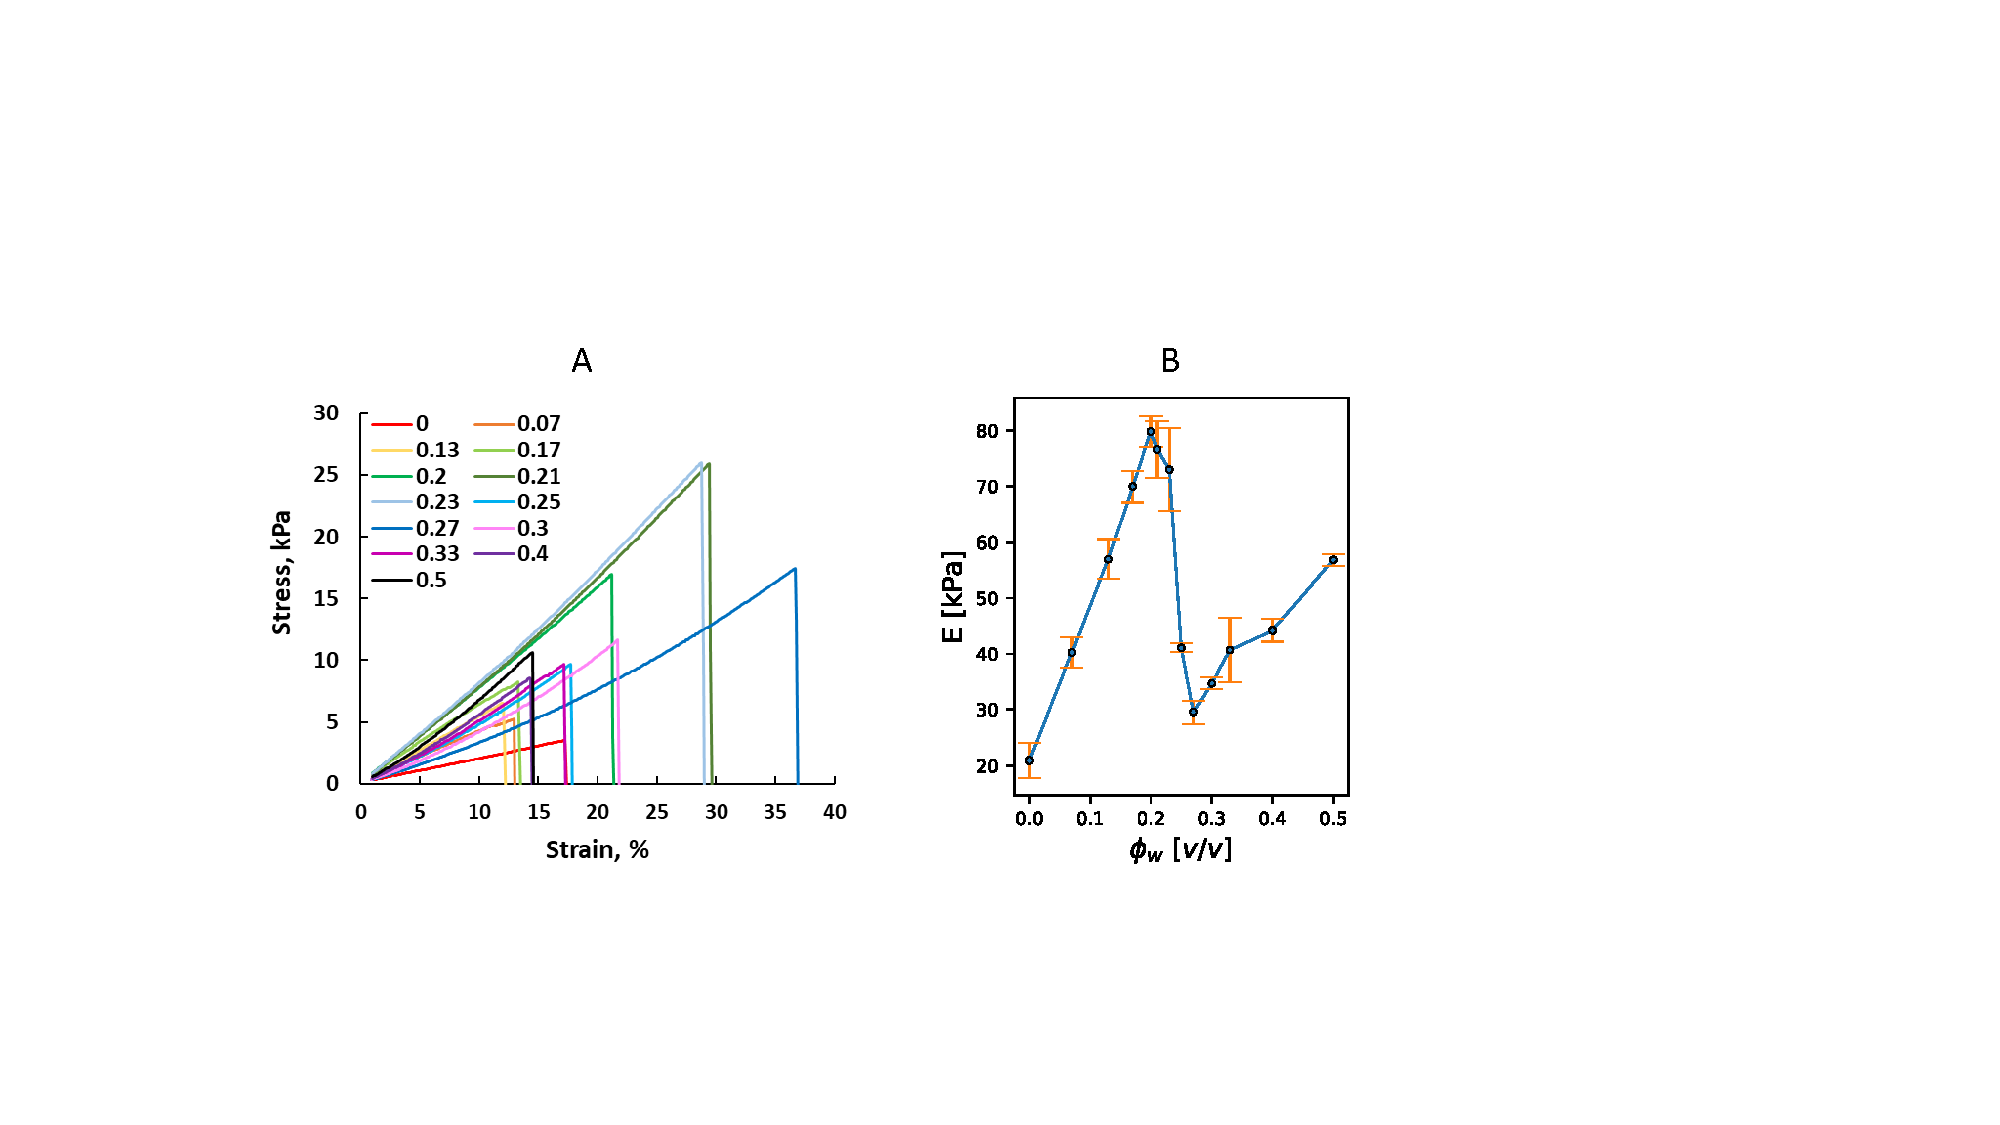
\includegraphics[width=\textwidth]{DMA.pdf}
      \caption{stress-strain curves (left) and derived Young’s modulus of the hydrogels as a function of water volume fraction ($\phi_{w}$).}
      \label{fig:DMA}
\end{figure*}

\begin{figure*}[!th]
      \centering
      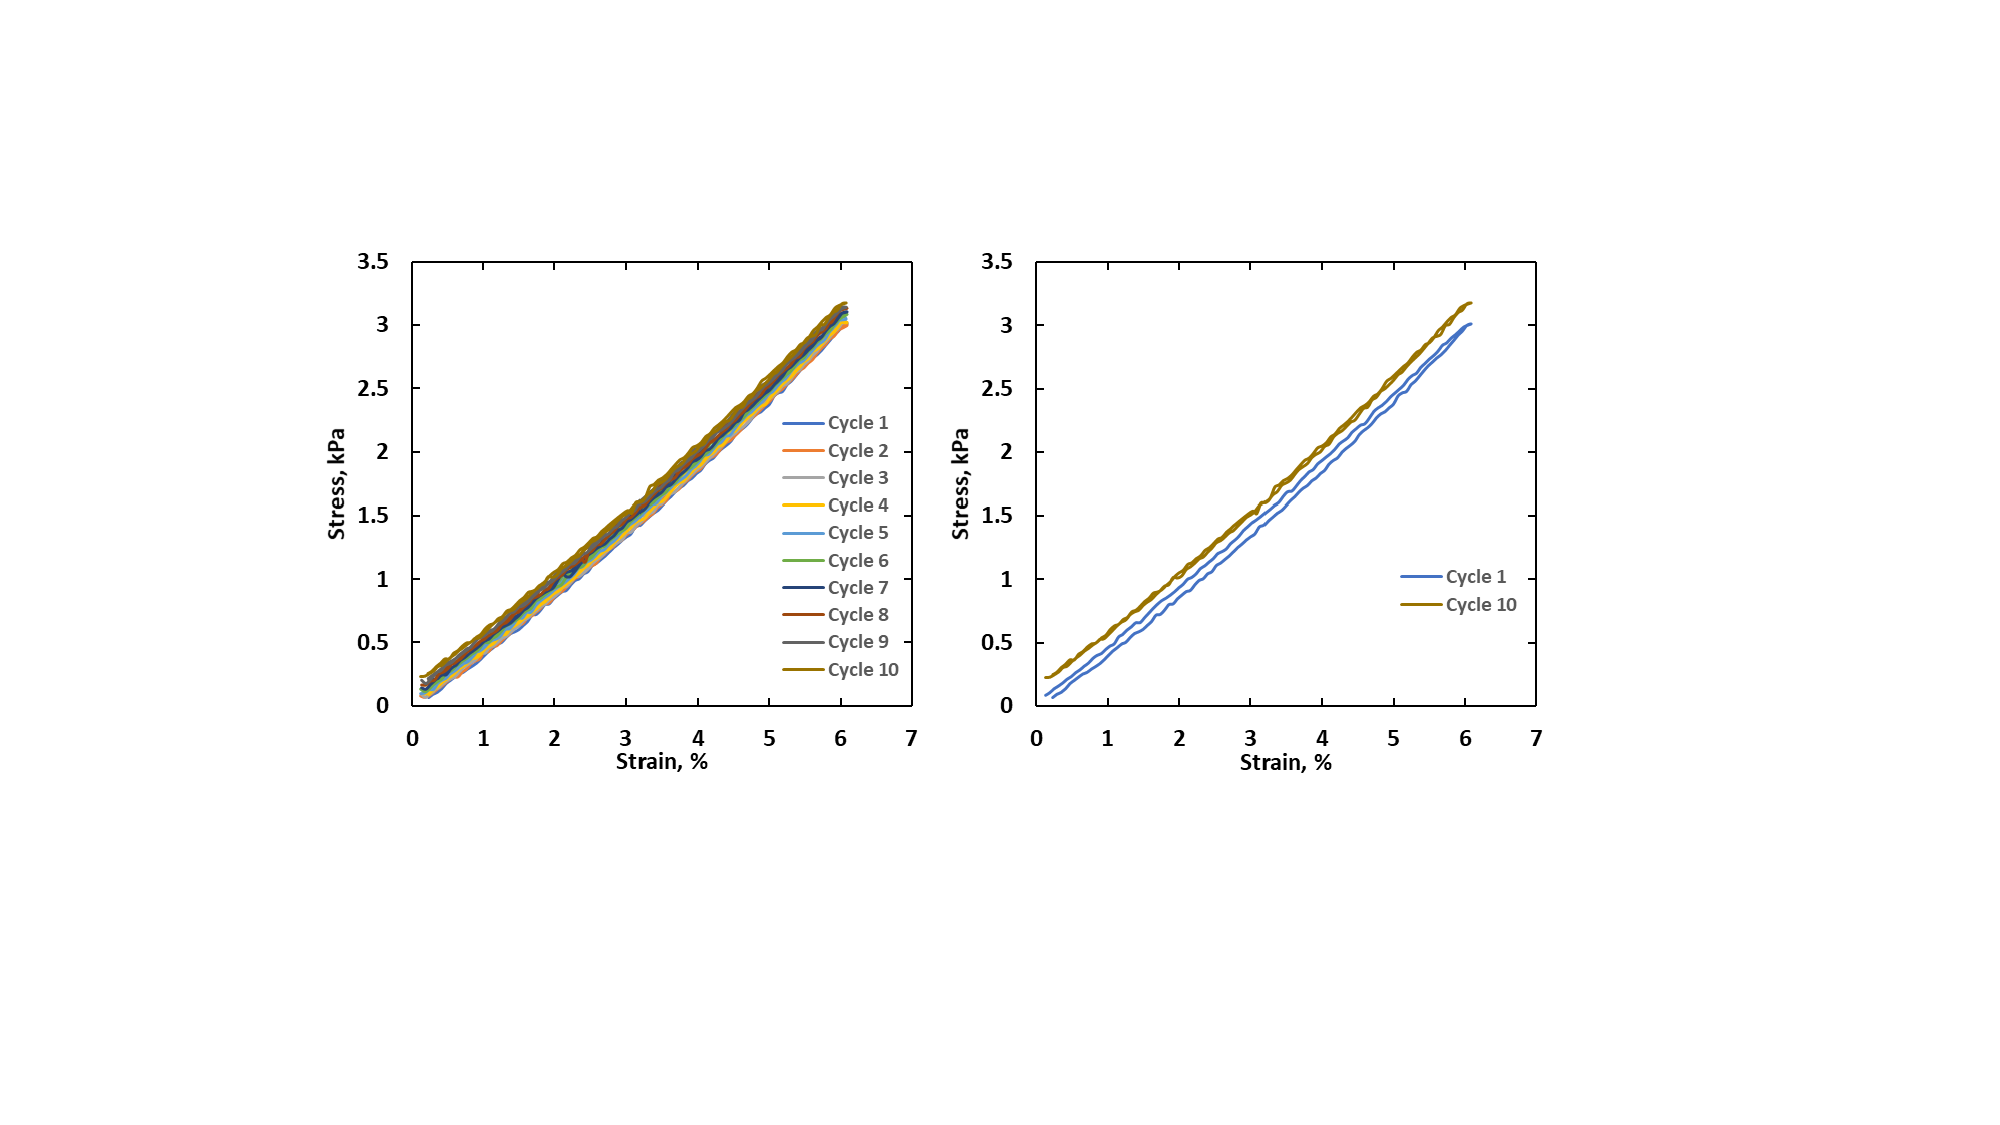
\includegraphics[width=\textwidth]{stressCycle.pdf}
      \caption{Stress-strain cycle test of HG03 ($\phi_{w}=0.3$) dogbone, demonstrating stability over 10 cycles (left). Stress-strain curves of Cycle 1 and Cycle 10, demonstrating a gradual shift upwards, due to drying-induced stiffening (right). A strain rate of $20\% min^{-1}$ is used to mitigate the effects of drying-induced stiffening.}
      \label{fig:stressCycle}
\end{figure*}

\subsection{Crosslink density using Flory theory}
The Flory-Rehner rubber elasticity theory provides a simple approach for calculating crosslink density from swelling measurements. The equation is as follows :
\begin{align}
	-[\ln⁡(1-\nu_2)+\nu_2+\chi_1 (\nu_2 )^2 ]=V_1 n[(\nu_2 )^{(\frac{1}{3})}-\frac{\nu_2}{2}]
\end{align}
%-[ln⁡(1-ν_2 )+ν_2+χ_1 (ν_2 )^2 ]=V_1 n[(ν_2 )^(1/3)-ν_2/2]
%\ln(w)
In the above, $\nu_{2}$ represents the volume fraction of the polymer in the hydrogel, $\chi_{1}$  represents the Flory-Huggins interaction parameter for PNIPAAm-water  which is equal to 0.5,  $V_{1}$ represents the solvent (water) molar volume ($18~cm^3~mol^-1$), and n represents the density of linear polymer segments bound by crosslinks on both ends. $\nu_{2}$ can be expressed in terms of the polymer volume ($V_polymer$) and gel volume ($V_gel$), as follows:
\begin{align}
	\nu_2=\frac{V_{polymer}}{V_{gel}} =\frac{(\frac{{m_polymer}}{\rho_{polymer}})}{V_{gel}} 
\end{align}

$V_{gel}$ can be measured directly from the dimensions of a regular-shaped hydrogel; m_polymer is the dry mass of this hydrogel after freeze-drying. The density of the polymer ($\rho_{polymer}$) can be measured via the following volume relationship:

\begin{align}
	V_{gel}=\frac{m_{water}}{\rho_{water}} +\frac{m_{polymer}}{\rho_{polymer}} 
\end{align}

This can be re-written in the following:
\begin{align}
	\rho_{polymer}=\frac{m_{polymer}}{(V_{gel}-\frac{m_{water}}{\rho_{water}})}
\end{align}

Here, $m_{water}$ represents the mass of the wet hydrogel minus $m_{polymer}$. With these relationships, $\nu_{2}$ for photo- and thermo-polymerized HG03 PNIPAAm can be calculated, and hence $n$ can be obtained. Furthermore, the average molecular weight of crosslinked polymer segments $(M_{c})$ can also be calculated using the following modified equation, assuming the hydrogel is composed of a completely continuous polymer network:

\begin{align}
	-[\ln⁡(1-\nu_{2} )+\nu_{2}+\chi_{1} (\nu_{2} )^{2}]=(\frac{V_{1}}{(\overline{\nu} M_{c})})[(\nu_{2} )^{(\frac{1}{3})}-\frac{\nu_{2}}{2}]
\end{align}

Here, $\overline{\nu}$ represents specific volume of the polymer in the hydrogel, represented by the following:
\begin{align}
\overline{\nu}=\frac{V_{gel}}{m_{polymer}} 
\end{align}
Table~\ref{table:flory} lists the key values of relevant properties calculated with this method.

\begin{table}[htbp]
\centering
\captionsetup{justification=centering}
\caption{Values of mass fraction of water, volume fraction of polymer, $n$, and $M_{c}$ for photo- and thermo-polymerized HG03 hydrogels.}\vspace{-0.25cm}
\begin{tabular}{c c c}
\hline
\hspace{-2mm}  & Photo & \hspace{-2mm} Thermo\\
%\hspace{-2mm} (mm) &  trajectory   & (g)  & (mm)& (mm)& (mm) & \hspace{-2mm}$\%$\\
\hline
\hspace{-2mm}$m_{water}$ & 0.87    & \hspace{-2mm}0.85\\
\hspace{-2mm}$V_{Polymer}$ & 0.26  & \hspace{-2mm}0.27\\
\hspace{-2mm}$n(\frac{mol}{cm^{3}})$ & $7.56 \times 10^{-4}$ & \hspace{-2mm}$9.37 \times 10^{-4}$\\
\hspace{-2mm}$M_{c}(\frac{g}{mol})$ & 149       & \hspace{-2mm}140\\
%\hspace{-2mm}9 & Half Ellipse      & - & 0.129 & 0.058 & 0.132 & \hspace{-2mm}9.8\\
%\hspace{-2mm}9 & Quarter Ellipse   & - & 0.161 & 0.061 & 0.171 & \hspace{-2mm}12.8\\
%\hspace{-2mm}25 & Ellipse          & 1 & 0.140 & 0.022 & 0.144 & \hspace{-2mm}8.9\\
%\hspace{-2mm}25 & Ellipse          & 2 & 0.162 & 0.021 & 0.162 & \hspace{-2mm}10.1\\
%\hspace{-2mm}25 & Ellipse          & 3 & 0.164 & 0.022 & 0.164 & \hspace{-2mm}10.2\\ 
\hline
\end{tabular}
\label{table:flory}
\vspace{-4mm}
\end{table}

\subsection{Scanning Elecron Microscope (SEM) Imaging}
To prepare SEM samples, each hydrogel prepolymer recipe was photopolymerized under UV light in a 1~mm$\times$5~cm$\times$7~cm PDMS mold to form sheets. After rinsing in DI water to remove DMSO and excess monomer, the sheets were cut into $1~mm$ thick slices. These slices were immersed in liquid nitrogen to instantly freeze and then immediately placed in a freeze-drier for 24 hours to remove the ice. The freeze-dried hydrogel slices were then imaged under SEM after sputtering a $5-10~nm$ layer of gold on them. The SEM images for hydrogels with different solvent ratio is shown in Figure~\ref{fig:compiledSEM}

\begin{figure*}[!th]
      \centering
      \includegraphics[width=\textwidth]{compiledSEM.pdf}
      \caption{SEM images of the hydrogel microstructure. The numbers indicate the water volume fraction ($\phi_w$). The scale bars are 10$\mu$m and 1$\mu$m for the low and high magnifications, respectively.}
      \label{fig:compiledSEM}
\end{figure*}

\subsection{Studying pore wall deformation mechanism}
We have taken additional SEM images for the HG03 in a shrunken state (Figure~\ref{fig:poreDeformation}) to see if there is any buckling of the pore walls. Although there might be some buckling observed, they happen at random direction and therefore, they do not result in directional contraction or expansion of the bulk gel which results in a negative Poisson’s ratio. In case of metamaterials in contrast, the buckling happens at microstructures that are ordered and patterned using micromanufacturing techniques such that they buckle all in the same direction resulting in the observed negative Poisson’s ratio.

\begin{figure*}[!th]
      \centering
      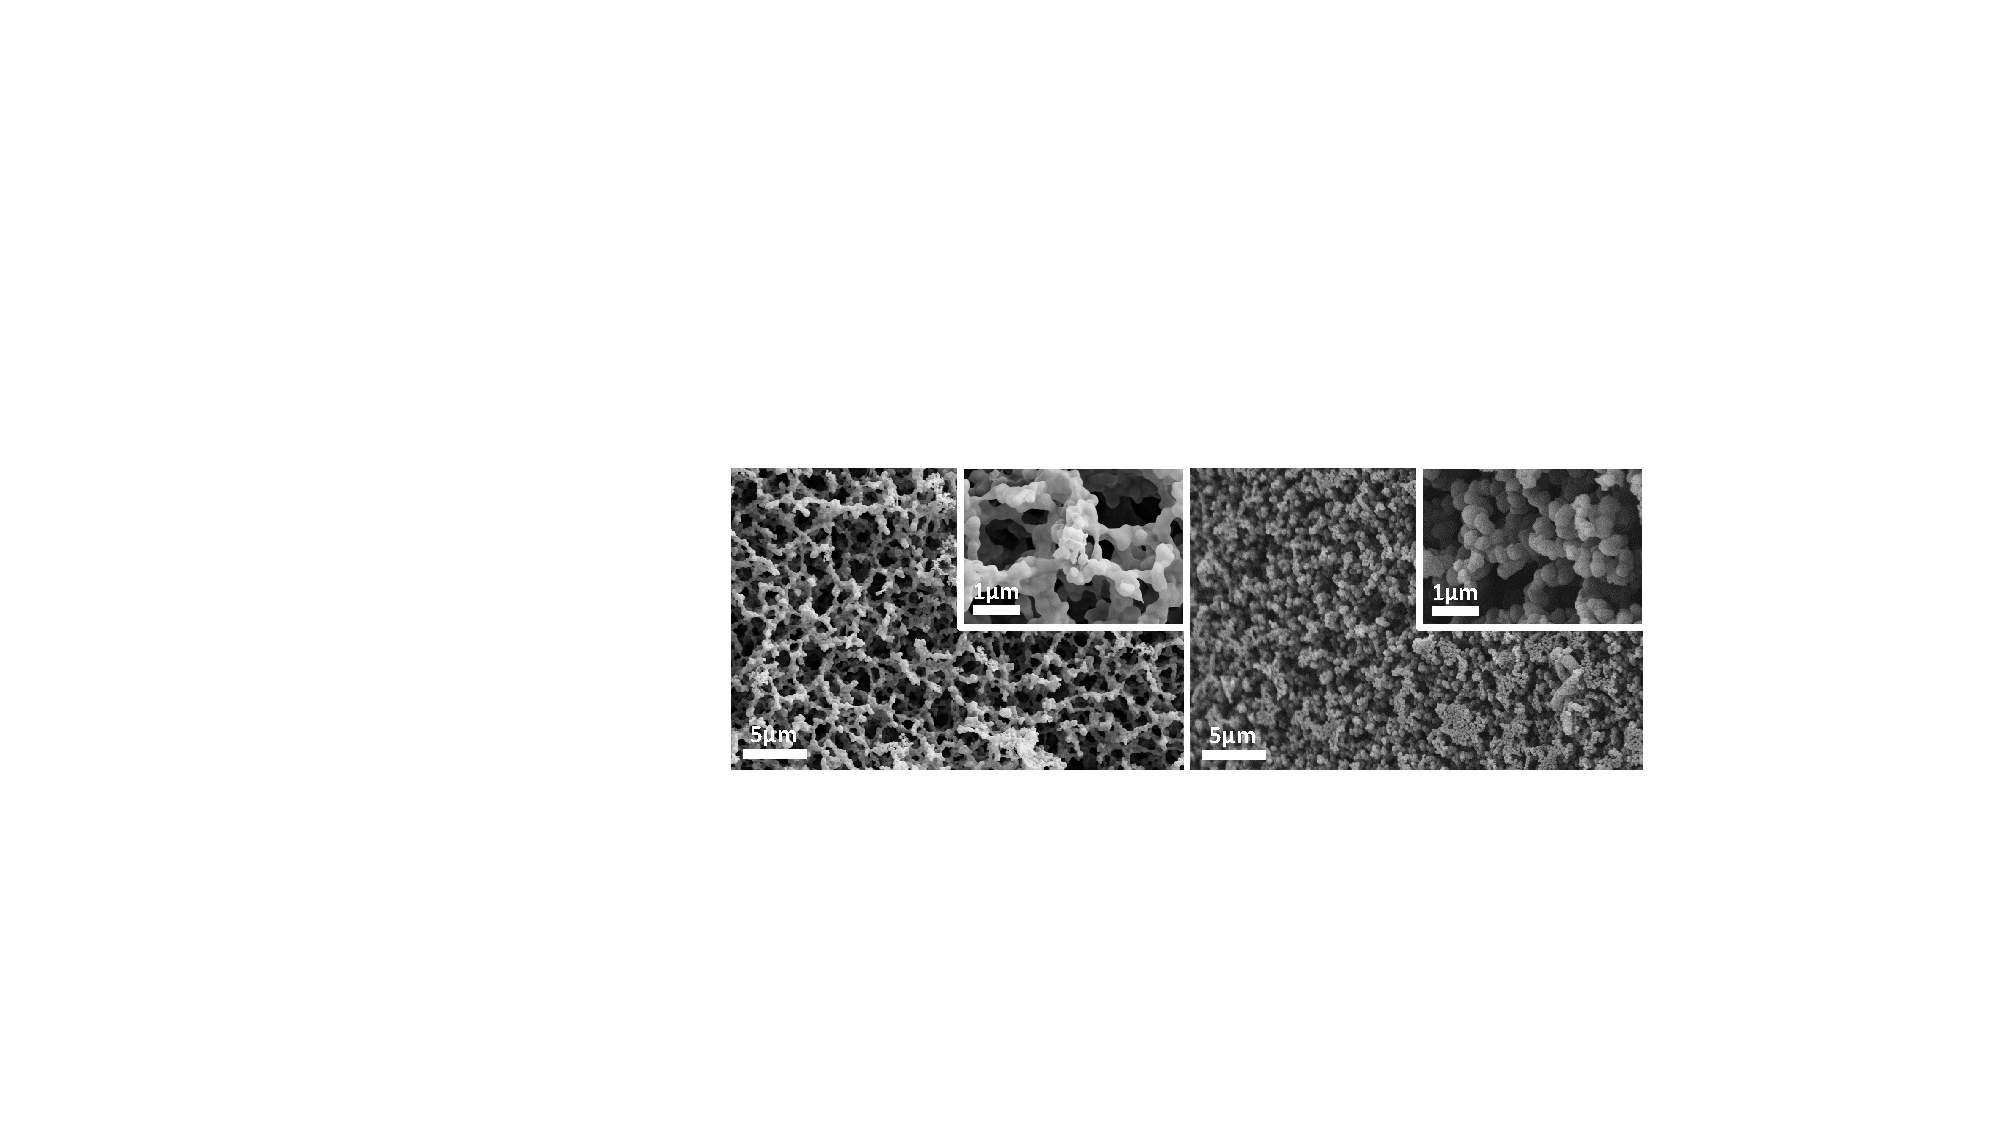
\includegraphics[width=\textwidth]{poreDeformation.pdf}
      \caption{SEM images of the HG03 hydrogel ($\phi_w$) in swollen state (left) and shrunken state (right).}
      \label{fig:poreDeformation}
\end{figure*}

\subsection{Studying the effect of freeze-thaw method on the pore structure and response of the hydrogel}
Based on our prior experience, a freeze-thaw post-treatment with conventional closed-pore PNIPAAm gels (prepared in pure DMSO) results in enhanced swelling performance since the ice crystals can grow and expand or break the close-walled pore boundaries, resulting in a greater degree of pore interconnectivity (Figure~\ref{fig:freeze}). However, with the open-porous PNIPAAm gel (HG03), as the SEM images in Figure~\ref{fig:freeze1} shows, the as-prepared HG03 gel and the gel freeze-thawed 5 times in a $-20^{o}C$ freezer do not show a significant difference in their pore structures.

\begin{figure*}[!th]
      \centering
      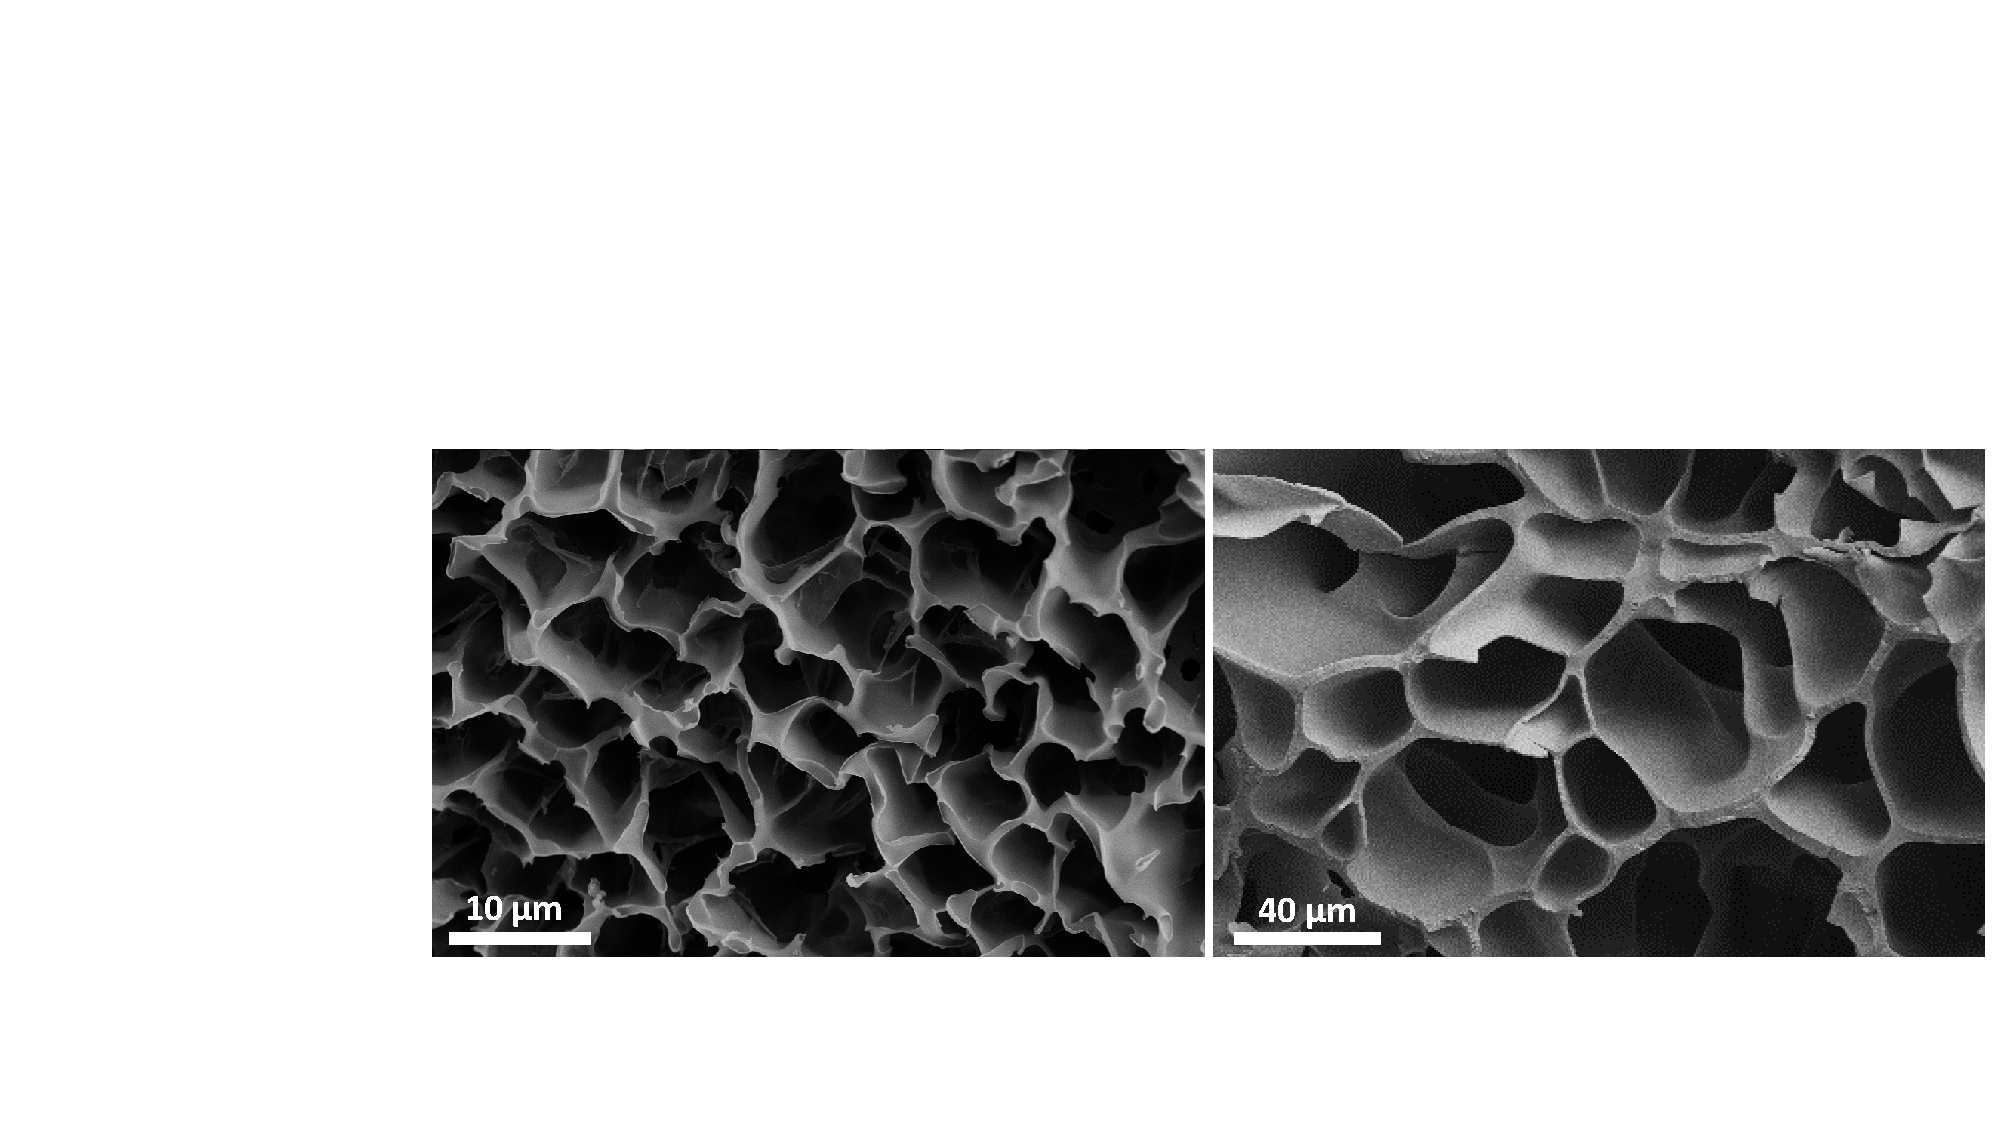
\includegraphics[width=\textwidth]{freeze.pdf}
      \caption{SEM images of as-prepared HG00 (left) and HG00 after a single freeze-thaw cycle (right). scale bars inside the figures are different.}
      \label{fig:freeze}
\end{figure*}

\begin{figure*}[!th]
      \centering
      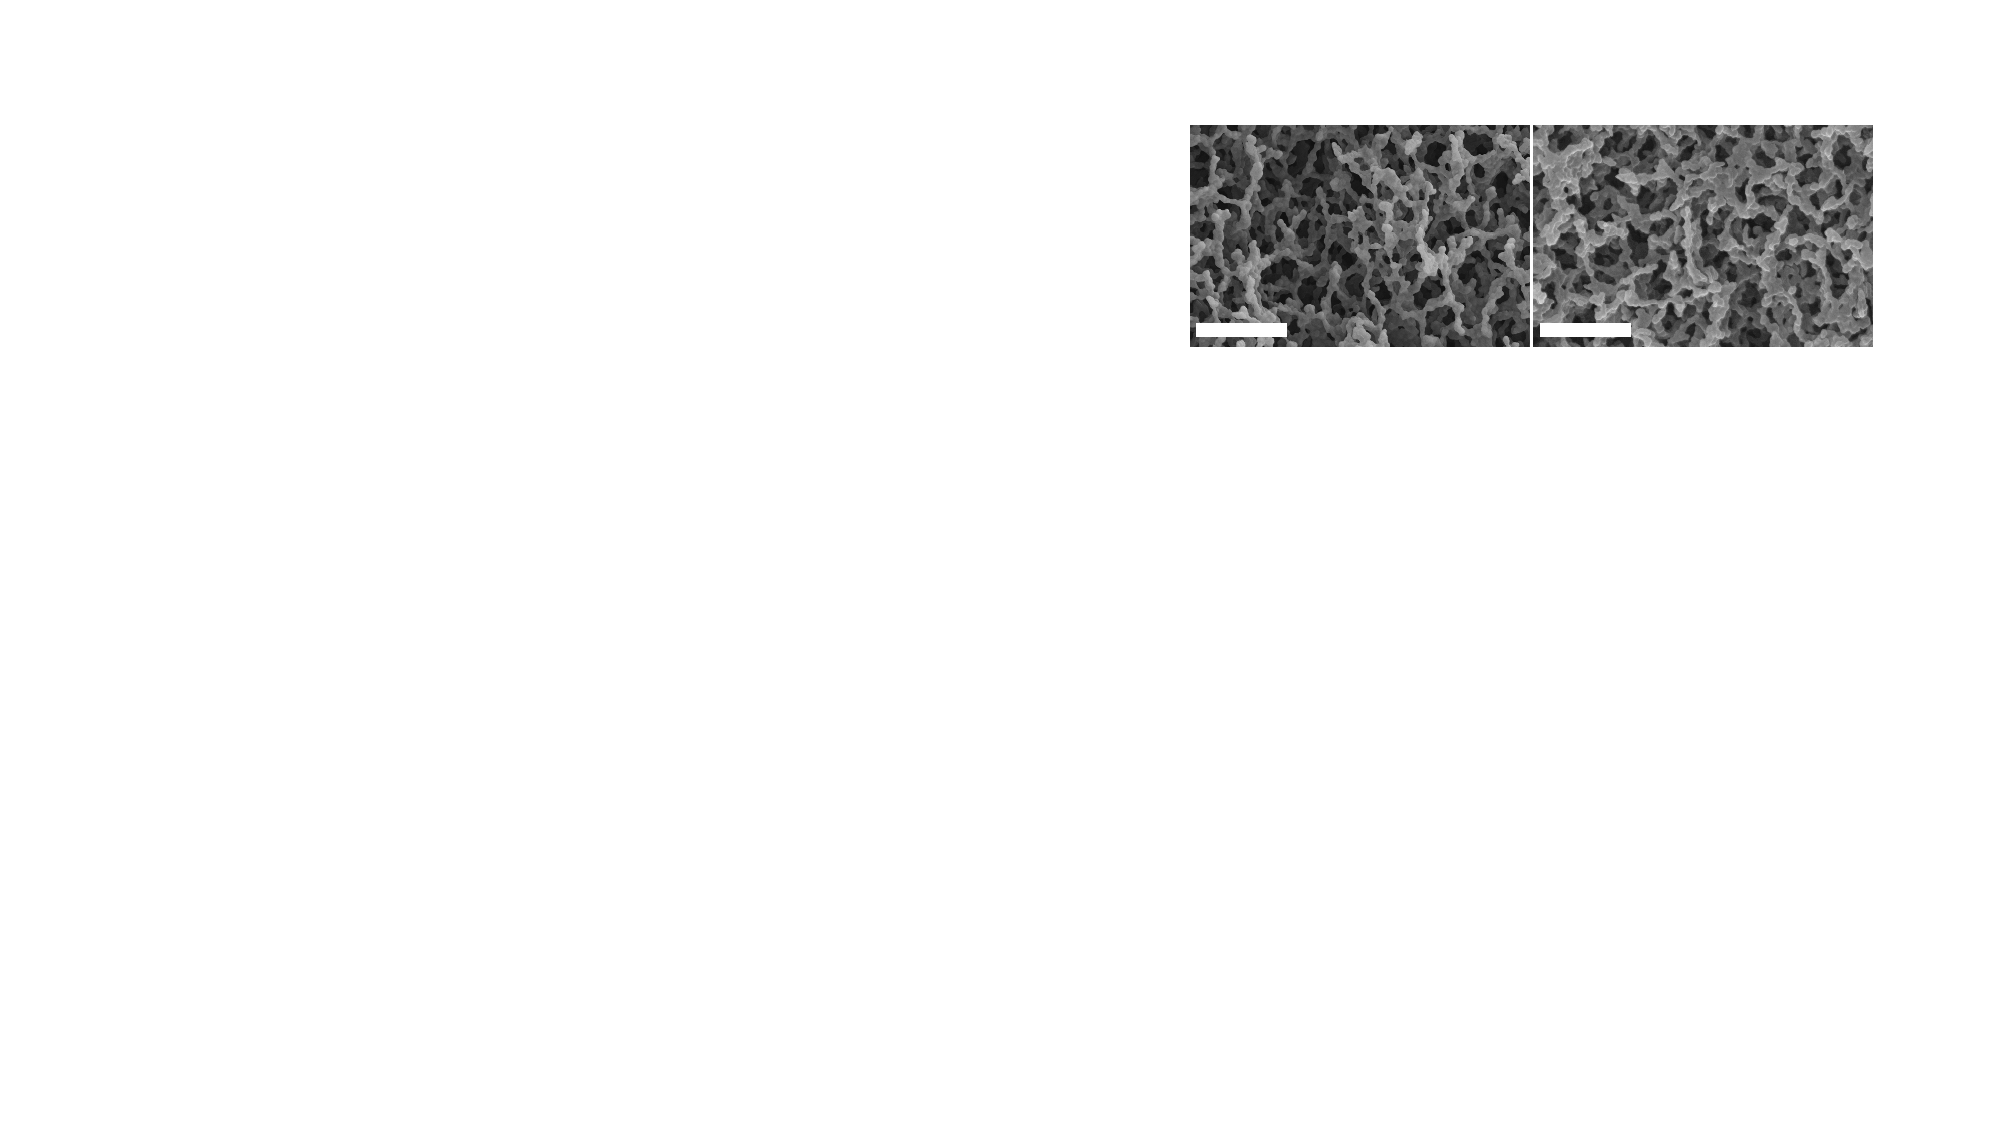
\includegraphics[width=\textwidth]{freeze1.pdf}
      \caption{SEM images of as-prepared HG03 (left)  and HG03 hydrogels after five freeze-thaw cycles (right). scale bars: $5\mu$m.}
      \label{fig:freeze1}
\end{figure*}

\subsection{Comparing photopolymerization swelling performance to thermopolymerization}
The photopolymerized PNIPAAm sample is fabricated by dissolving $400~mg$~$mL^{-1}$ NIPAAm and $20~mg$~$mL^{-1}$ BIS into $2~mL$ of DMSO-water mixed solvent (0.27 vol fraction DMSO). $5\mu$L~$mL^{-1}$ of Darocur 1173 is added as the photoinitiator and vortexed thoroughly. The prepolymer solution is pipetted into a PDMS mold with dimensions $1~cm$$\times$$1~cm$$\times$$1.5~mm$ and illuminated with UV light for 15s to induce gelation. The photopolymerized PNIPAAm hydrogel is removed from the mold and allowed to soak in DI water for 24 hours to remove unreacted precursors and DMSO. The thermopolymerized PNIPAAm sample is fabricated by dissolving $400~mg$~$mL^{-1}$ NIPAAm and $20~mg$~$mL^{-1}$ BIS into $2mL$ of DMSO-water mixed solvent (0.27 vol fraction DMSO). $20~mg$~$mL^{-1}$ ammonium persulfate thermoinitiator is added, followed by vortexing until fully dissolved. This precursor is then chilled in a $-5^{o}C$ fridge for 15\,min, prior to adding $20~\mu$L~$mL^{-1}$ TEMED. After briefly inverting the precursor container several times to facilitate TEMED mixing, the precursor is pipetted into a PDMS mold with dimensions $1~cm$$\times$$1~cm$$\times$$1.5~mm$ and allowed to react for 15 hours. The thermopolymerized PNIPAAm hydrogel is removed from the mold and allowed to soak in DI water for 24 hours to remove unreacted precursors and DMSO.
To confirm that thermopolymerized PNIPAAm synthesized under these reaction conditions serves as an adequate control for the photopolymerized PNIPAAm, the reaction conversion is measured. The conversion quantifies how much of the dissolved precursor is consumed in the polymerization reaction, and is defined as follows, where W_dry  is the weight of the dry hydrogel, C_solute  is the total concentration of dissolved monomer and crosslinker, and V_mold  is the volume of the hydrogel mold:
\begin{align}
	Conversion = \frac{W_{dry}}{(C_{solute}×V_{mold} )}\times~100
\end{align}

Additionally, water content is measured to further validate that the thermopolymerized PNIPAAm synthesized under the above conditions serves as a comparable control. 
\begin{align}
	Water~Content = \frac{(W_{wet}-W_{dry})}{W_{wet}}\times~100
\end{align}

The matching conversion and water content for the photopolymerized and thermopolymerized PNIPAAm hydrogels indicate that the two can be compared directly.

\subsection{Effect of environmental conditions on SVA performance}
We have studied the effect of environment temperature on SVA performance by measuring the SVA force as the temperature of the water bath is varied. Figure~\ref{fig:envTemp} shows the SVA force as it is turned on for 60 s and off for 60 s for a total of 10 cycles.
\begin{figure*}[!ht]
      \centering
      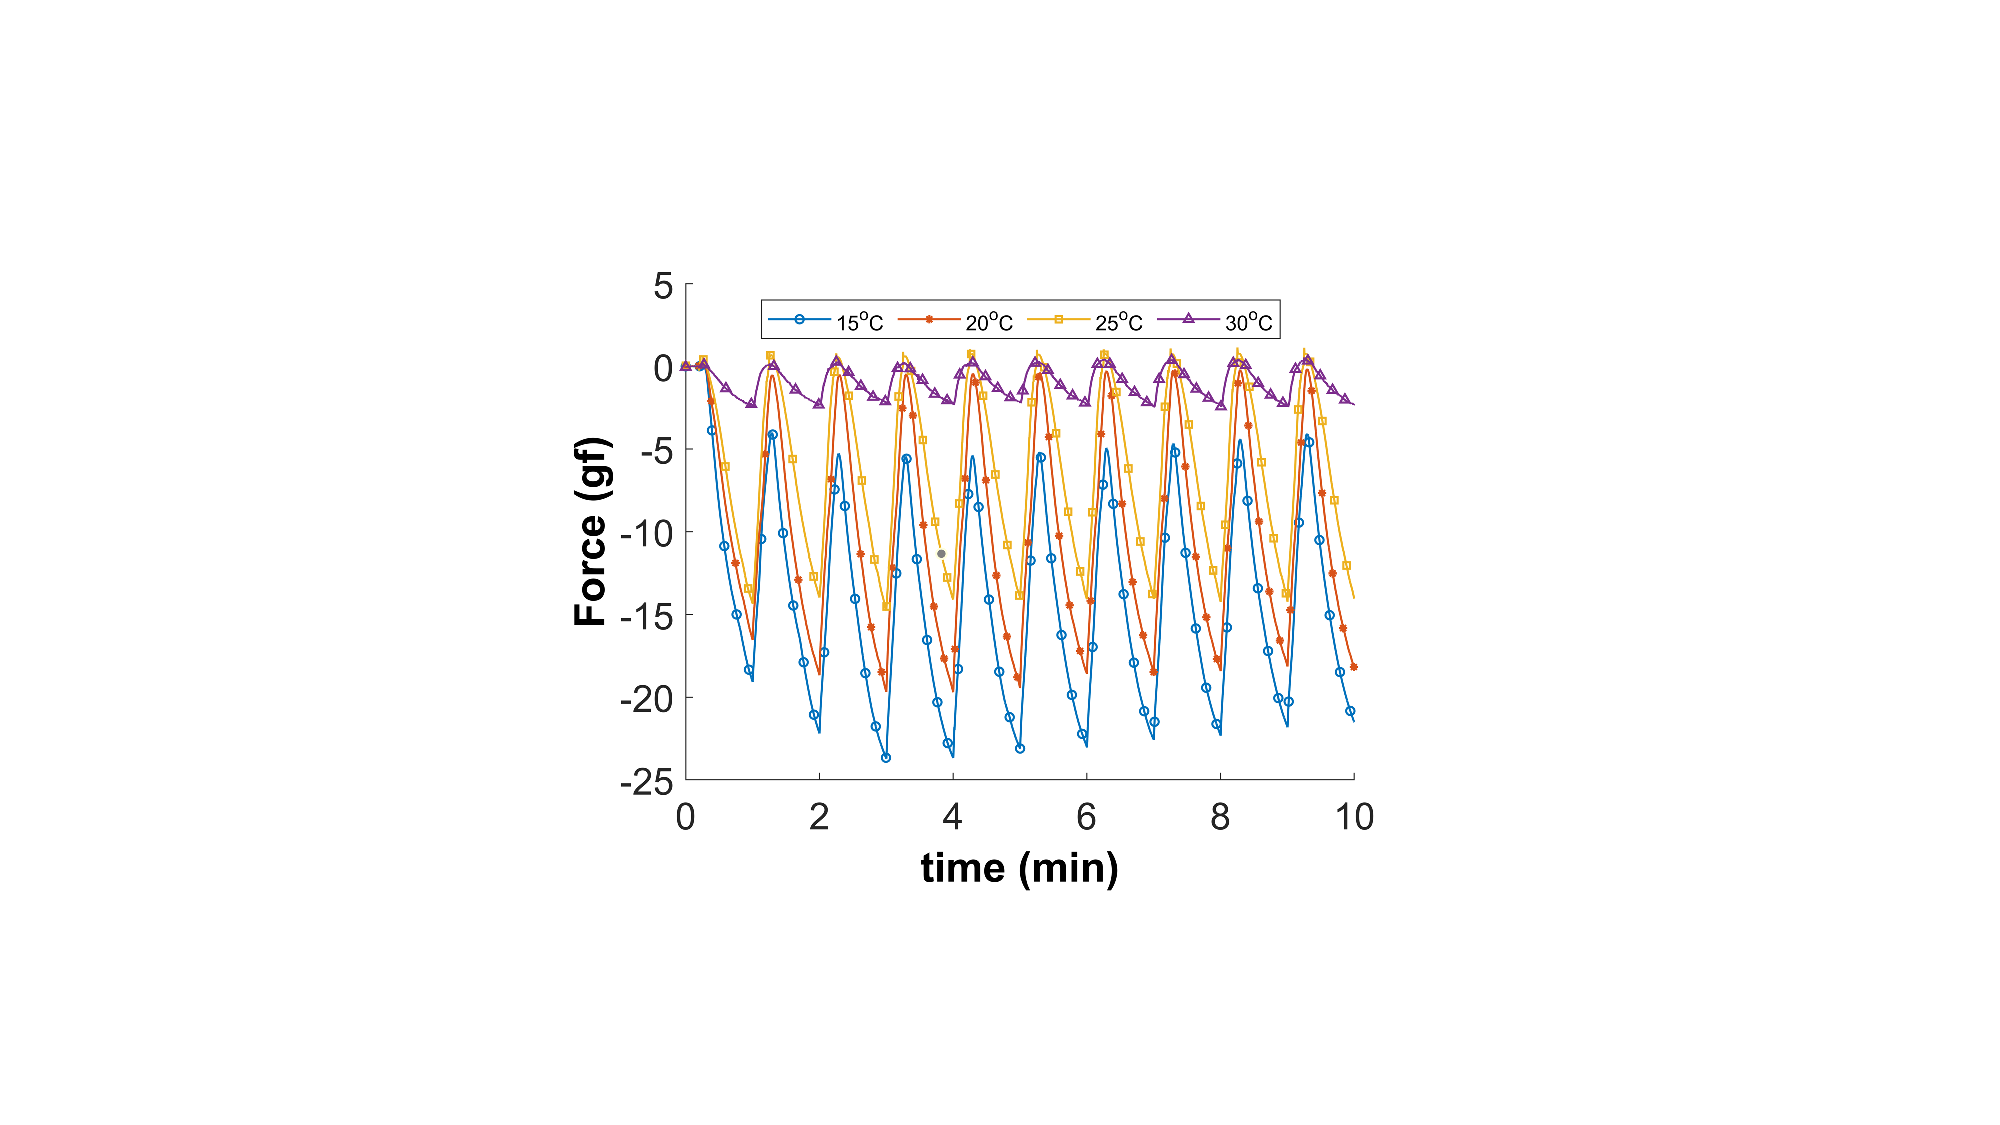
\includegraphics[width=0.8\textwidth]{envTemp.pdf}
      \caption{Effect of the temperature of the water bath on the force production capacity of the SVAs.}
      \label{fig:envTemp}
\end{figure*}

\subsection{Cyclic tests}
We have characterized the long-term performance of the SVAs as they go through multiple cycles of expansion/contraction. The SVAs used for this test have not been gone through any heating and cooling cycles prior to this test. Figure~\ref{fig:cyclicDisp} shows the displacement over 1000 cycles. The temperature change dynamics is also measured by placing a thermocouple inside the SVA. As can be seen, the amplitude of the force is almost the same throughout the time. There is a very small drift which can be related to the settling of the force sensor setup over time. To further evaluate this, the SVA force in the first cycle is plotted against the last cycle. There is a slight improvement in the amplitude of the force and the SVA response seems to be slightly faster. We think this is due to the removal of residual DMSO, monomer and non-crosslinked polymer molecules from the gel when it is initially actuated. Overall, the SVAs does not show significant change in their performance over cyclic loads. 
\begin{figure*}[!htb]
      \centering
      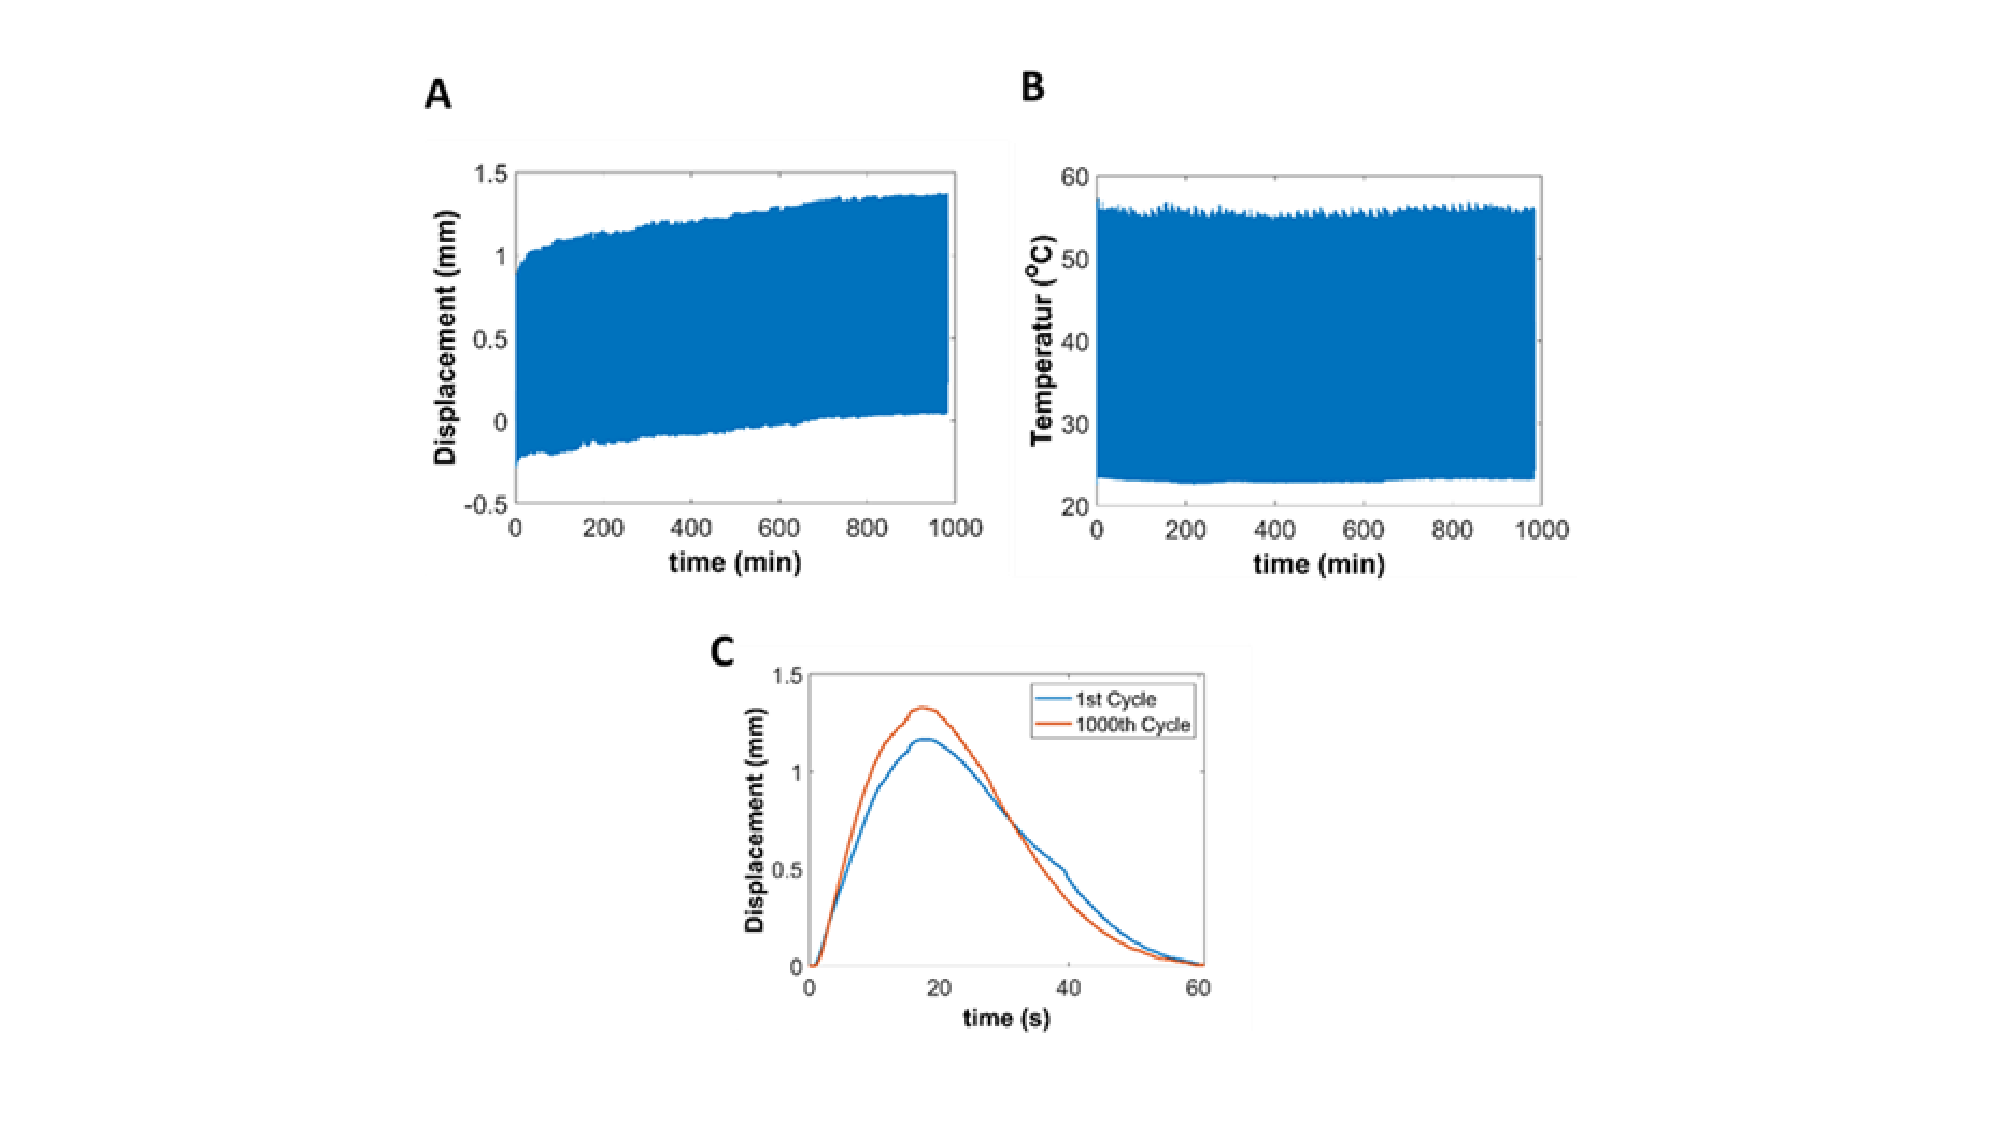
\includegraphics[width=0.8\textwidth]{cyclicDisp.pdf}
      \caption{A) Displacement of SVA over 1000 activation cycles. B) The temperature inside the SVA is also plotted. C) the displacement during first cycle and last cycle plotted for comparison.}
      \label{fig:cyclicDisp}
\end{figure*}

\subsection{Dependency of the performance of SVAs on their size}
As the volume change of hydrogel depends on temperature, the larger the size of the SVAs are, more time is needed for them to heat up by the Joule heaters and reach their minimum shrunken volume. To quantify this, we have tested 3 SVAs with different sizes and measured the displacement produced as the heater is turned on for 60 s and off for 60 s for a total of 10 cycles. As can be seen in Figure~\ref{fig:svaSize}, the larger SVAs produced higher deformation, however they need more time to reach that deformation. 
\begin{figure*}[!htb]
      \centering
      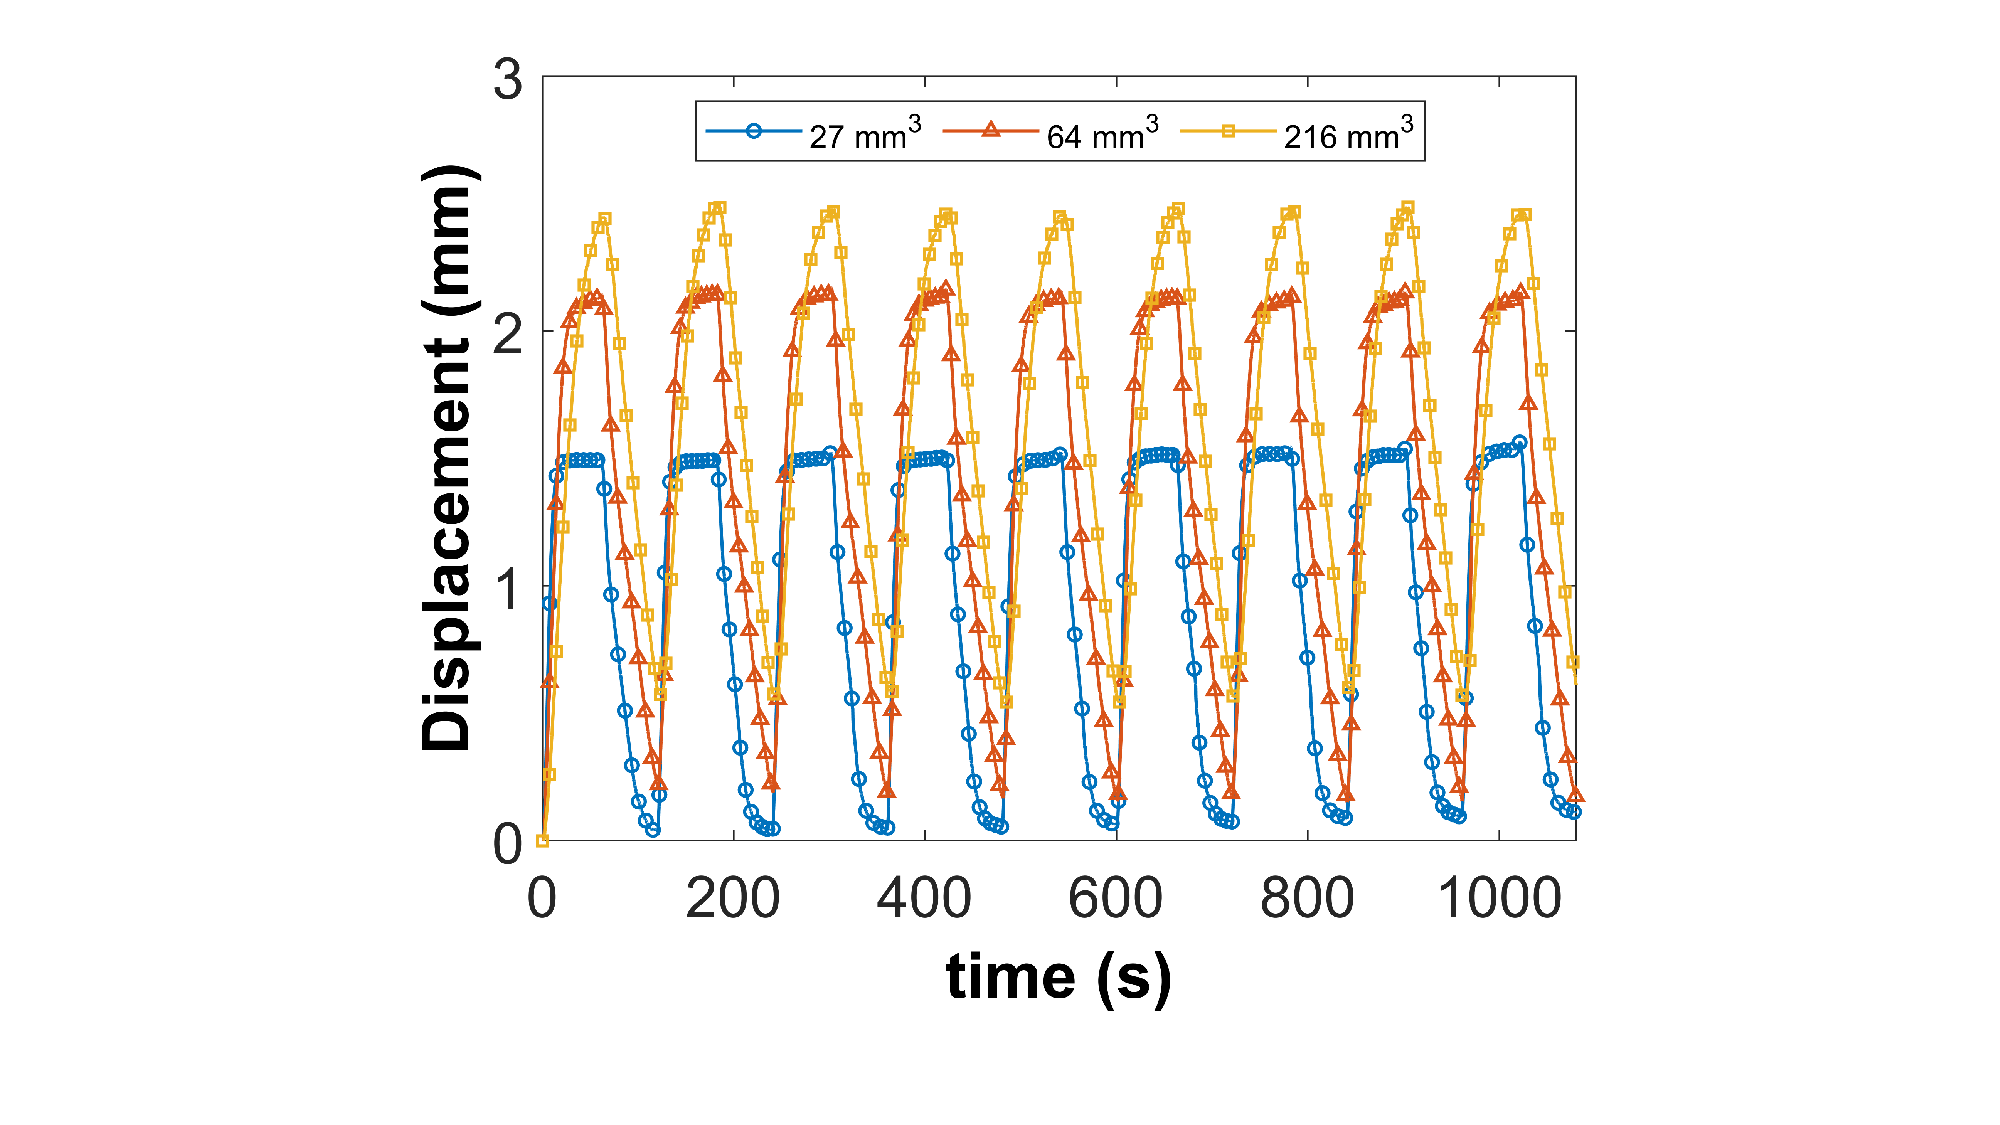
\includegraphics[width=0.6\textwidth]{svaSize.pdf}
      \caption{The effect of SVA size on the displacement produced as the heater is activated for 10 cycles.}
      \label{fig:svaSize}
\end{figure*}

\subsection{Kinetics of temperature change} 
In order to quantify the temperature of an SVA, a thermocouple is placed inside a SVA made of H03, close to the Joule heater as shown in Figure~\ref{fig:tempKinetics}. The temperature and displacement profiles as the heater is turned on for 15~s and then turned and kept off for 45~s are plotted for comparison.

\begin{figure}[!htb]
\centering
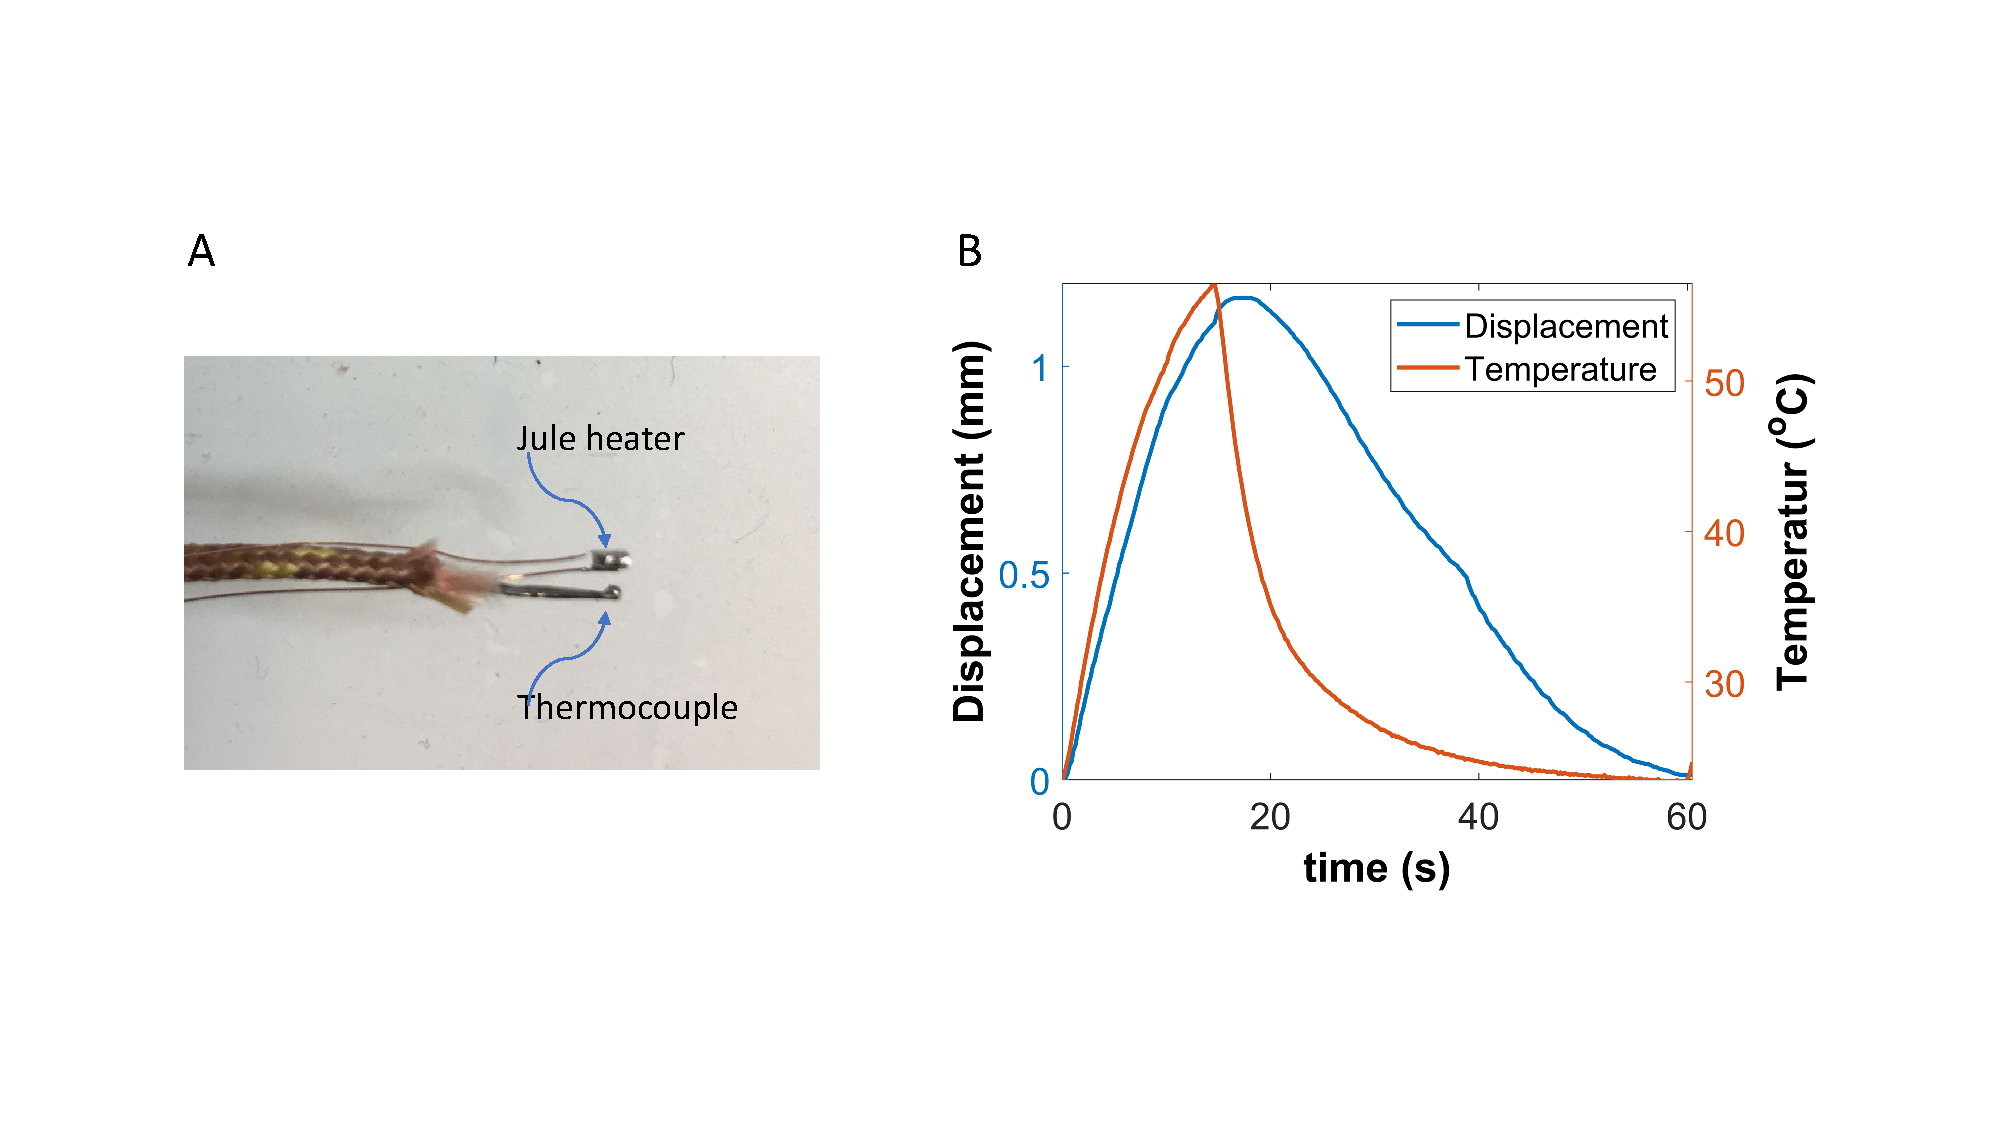
\includegraphics[width=\textwidth]{tempKinetics.pdf}
    \caption{A) the thermocouple is placed inside a SVA to measure the kinetics of the temperature change. B) temperature and displacement profiles }
    \label{fig:tempKinetics}
\end{figure}

%\begin{figure*}[!htb]
      %\centering
      %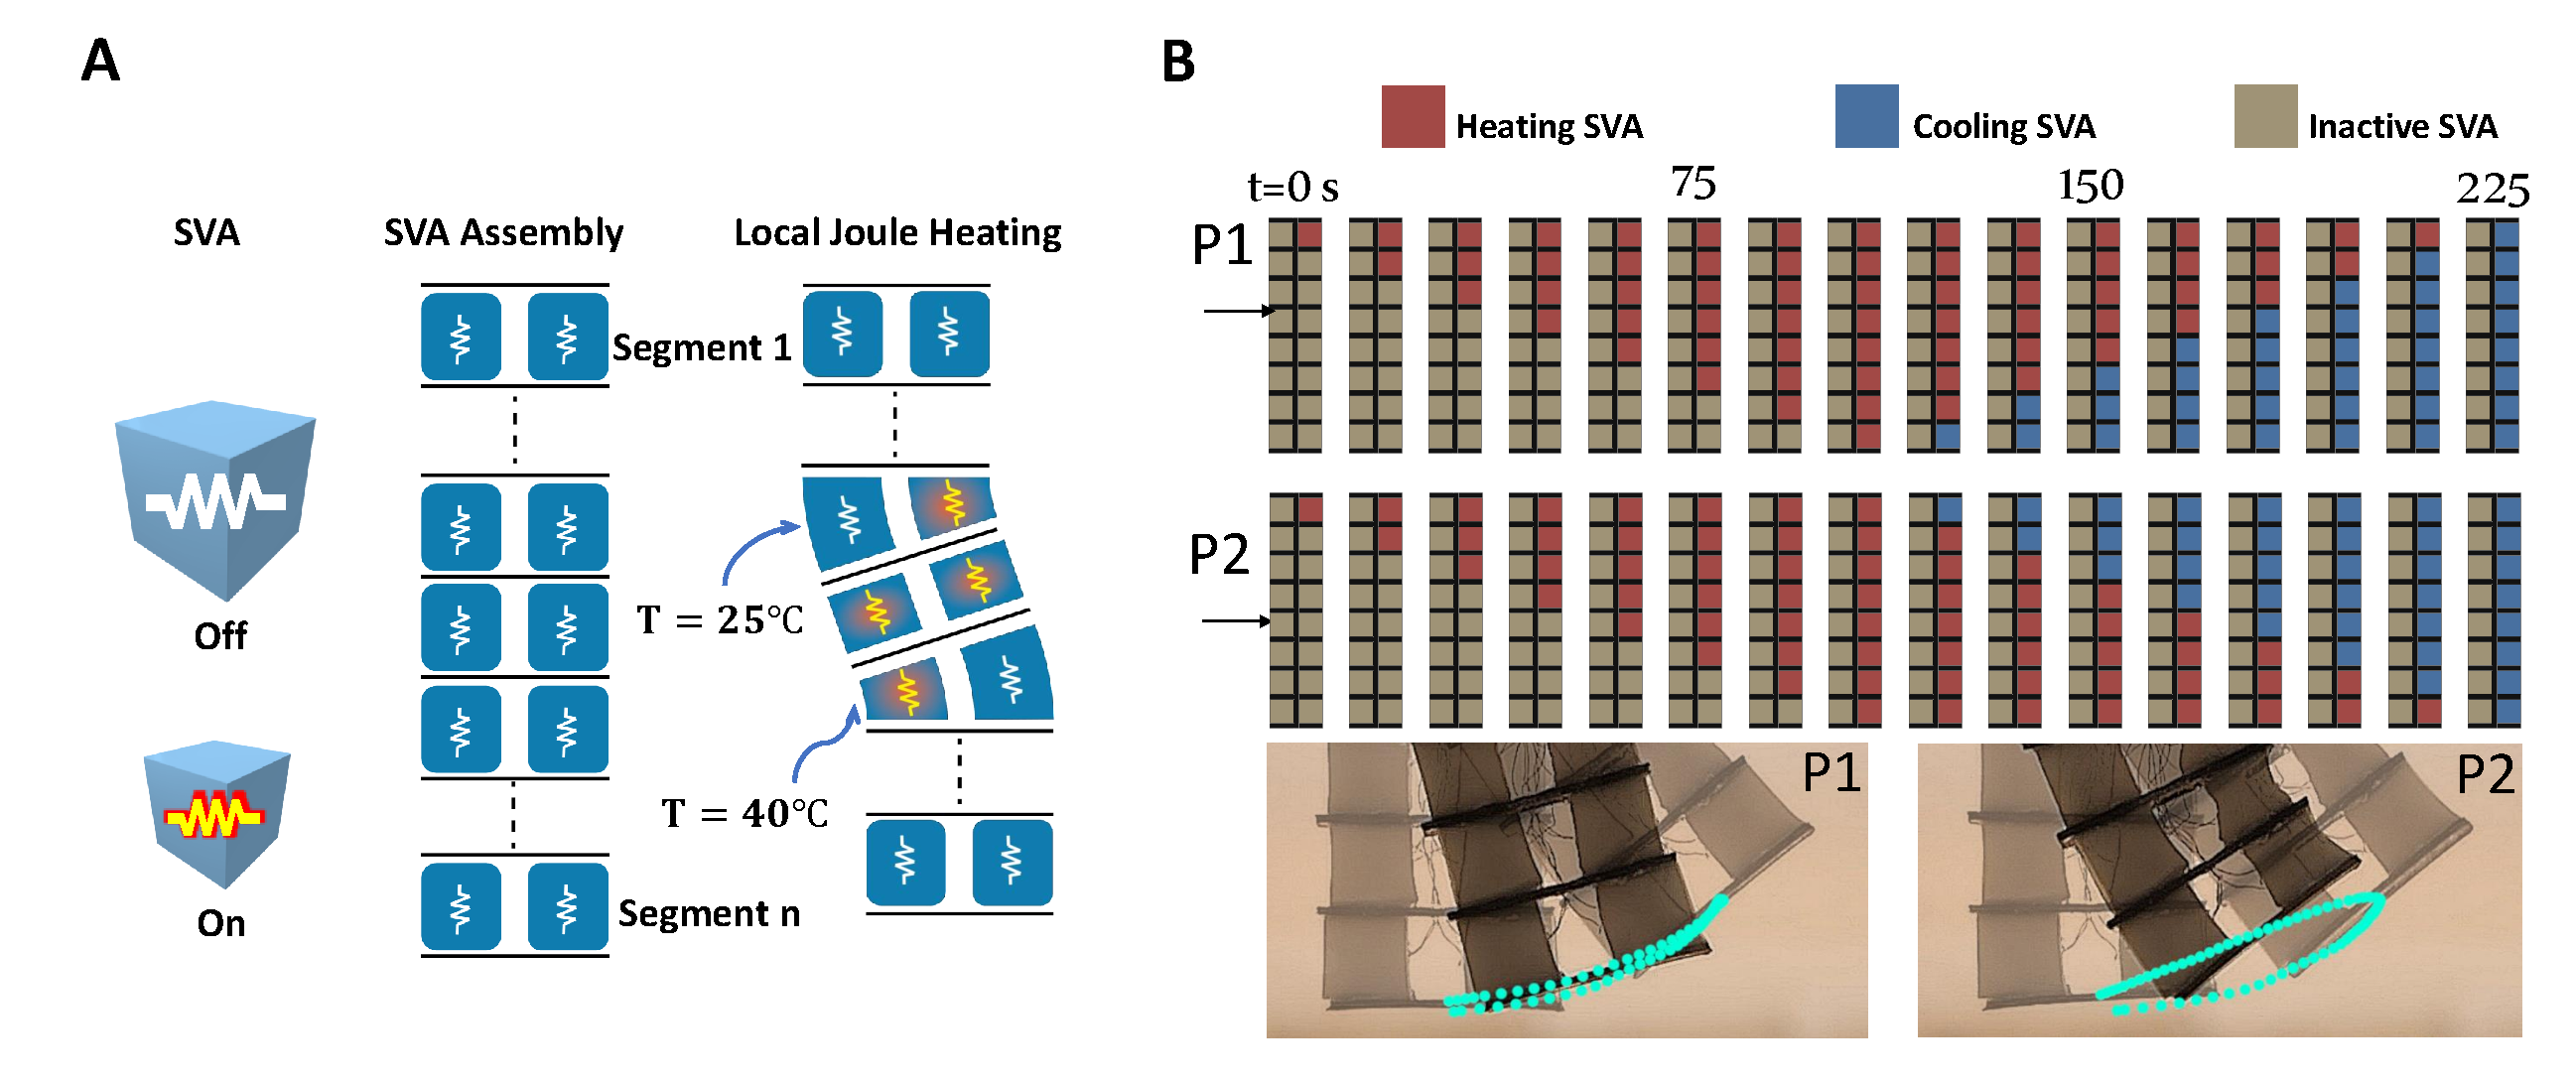
\includegraphics[width=\textwidth]{Fig2.pdf}
      %\caption{A) On and off states of a SVA is shown on the left column. Schematic of an assembly of SVAs is shown on the middle column. Activation of SVAs results in local increase in the temperature which leads to deformations that control the overall motion of the manipulator (right column). B) Sequentially activating SVAs 1 through 8 according to the patterns labeled P1 and P2 results in different trajectories followed by the tip of the manipulator (shown in cyan at the bottom). For details, see Movie S1.}
      %\label{fig:treajectory}
   %\end{figure*}
\graphicspath{{Images/heterogeneous/}}

\chapter{Heterogeneous hydrogel structures as Miniature Hyper-redundant Soft Manipulators}
\label{chap:heterogeneous}
Stimuli-responsive hydrogels can sense environmental cues and change their volume accordingly without the need for additional sensors or actuators. This enables a significant reduction in the size and complexity of resulting devices. However, since the responsive volume change of hydrogels is typically uniform, their robotic applications requiring localized and time-varying deformations have been challenging to realize. Here, using addressable and tunable hydrogel building blocks – referred to as Soft Voxel Actuators (SVAs) –heterogeneous hydrogel structures with programmable spatiotemporal deformations is presented. SVAs are produced using a mixed-solvent photopolymerization method, utilizing a fast reaction speed and the cononsolvency property of PNIPAAm to produce highly interconnected hydrogel pore structures, resulting in tunable swelling ratio, swelling rate, and Young’s Modulus in a simple, one-step casting process that is compatible with mass production of SVA units. By designing the location and swelling properties of each voxel and by activating embedded Joule heaters in the voxels, spatiotemporal deformations are achieved which enables heterogeneous hydrogel structures to manipulate objects, avoid obstacles, generate traveling waves and morph to different shapes. Together, these innovations pave the way towards tunable, untethered, and high degree-of-freedom hydrogel robots that can adapt and respond to changing conditions in unstructured environments.
\section{Background}
Smart hydrogels have attracted great interest in many different fields, such as drug delivery \citesuperscript{Annabi2014, Stuart2010},               
microfluidics \citesuperscript{DEramo2018a,Goy2019}, and soft robotics \citesuperscript{Banerjee2018}, owing to their large and reversible volume changes in response to a broad range of stimuli without using any additional sensors and actuators. This feature helps reduce the size of devices made of smart hydrogels. 
% \note{stimuli responsive are responsive to stimuli}. 
Practical soft robotic applications, ranging from basic bending and shortening primitives to complex reconfigurations, all require time-varying and local deformations of bulk hydrogels in order to approach the dexterity of 
% better mimic  the functions of 
soft organisms in performing tasks such as grasping and manipulation \citesuperscript{Ionov2014, Erol2019}.
However, the responsive volume change of smart hydrogels is typically uniform.
% \dma{\sout{to achieve precise and complex reconfigurations}}
Two main approaches have been adopted by researchers to achieve nonuniform spatiotemporal deformation in hydrogels \citesuperscript{Ionov2014}. In the first approach, heterogeneous structures in the shape of sheets and rods are fabricated by patterning material domains using manufacturing techniques such as micro- and meso-patterning \citesuperscript{Zhou2018b,Klein2007,Kim2012,Ma2016a,Erb2013,Huang2017} and 3D printing \citesuperscript{Zheng2018}. Differing swelling properties of neighboring domains upon stimulation results in nonuniform strain fields in these structures, causing them to transform into a variety of complex shapes like coils and conical helices \citesuperscript{Wu2013,Liu2016}.
% Zhou2018b,Peng2018,Lee2014,Ma2016a,Erb2013,Huang2017 of different swelling properties. Nonuniform strains develop across the \dma{\sout{bulk}} material as a result of the difference in amount of swelling of these domains. 
% Fabrication techniques used for patterning material domains include micro- and meso-patterning\citesuperscript{Zhou2018b,Peng2018,Lee2014,Ma2016a,Erb2013,Huang2017} and 3D printing.
% %may be used to create these patterns,
% \citesuperscriptsuperscript{Zheng2018} Basic shapes such as sheets and rods, when stimulated, can transform into a variety of complex shapes like coils and conical helices. \citesuperscriptsuperscript{Wu2013,Liu2016}\note{split into cones and conical refs?} 
The range of compatible materials available for each domain, however, is often limited by practical fabrication constraints, such as ink viscosity for 3D printing \citesuperscript{Zheng2018}. Moreover, the geometry and material selected for each domain determine the shape transformations; these features cannot be changed after manufacturing, making on-demand reconfiguration infeasible.\\
% and a new structure should be manufactured for each task.
% hard-codes structural shape transformation, .
%the configuration and material properties of the patterned domains in these structures. 
%Thus, after fabrication, the entire material deforms in a predefined manner in response to a global stimulus. On-demand shape transformations are therefore not feasible using these structures and a new structure should be manufactured for each task. 
%available within each domain
%which can be used for each domain 
%is limited due to fabrication constraints. The viscosity of hydrogel monomer solutions, for example, must be tuned to be compatible with some 3D printing techniques.\note{\citesuperscript{Zheng2018}}\note{make more compact}

The second approach towards achieving nonuniform spatiotemporal deformations uses an inhomogeneous or time-varying stimulus, such as patterns of structured light \citesuperscript{Palagi2016}, local irradiation by near-infrared light \citesuperscript{Mourran2017}, or localized electric fields \citesuperscript{Choi2020}. In these methods, the hydrogel material itself is typically homogeneous, but the stimulus intensity varies across different regions, causing localized and time-varying deformations. These techniques, while suitable for on-demand shape reconfiguration, often require bulky external equipment, ultimately leading to challenges in mobile robot applications.\\
%applications. Hence, in these approaches, the limited design flexibility and spatiotemporal re-programmability have remained key challenges for realizing complex motion in soft robotic tasks.

Nature has adopted a hierarchical approach in addressing these challenges by using motor units as building blocks for heterogeneous muscle tissue demonstrating complex spatiotemporally reprogrammable deformations  \citesuperscript{frontera2015, drost2003}. A motor unit consists of a motor neuron and the muscle fibers innervated by its axonal terminals \citesuperscript{buchthal1980}.
% , as shown in \firstsubfigref{fig:1}{A, right}.  
% it is a  in biological systems such as octopuses, caterpillars, and worms 
It behaves as a stimuli-responsive building block, producing unidirectional deformation in response to electrical stimulus from the central nervous system (CNS). 
% or peripheral nervous system (PNS) 
The variations in orientation \citesuperscript{KIER1985}  and response rate \citesuperscript{Kier1992} of muscle fibers create the structural heterogeneity \citesuperscript{Liu2017b} required for nonuniform hard-coded deformations; the on-demand control over location and intensity of the electrical stimulus provides the spatiotemporal reprogrammability \citesuperscript{Hanassy,Kazakidi2015,Richter2015}.\\
 
Virtual voxels have been used for decades as building blocks to represent shapes in 3-D space for computer graphics applications \citesuperscript{Yagel1993}.
% are shown to have the potential as building blocks for simulating and manufacturing heterogeneous structures. 
More recently, voxel-based simulations have been used to predict bulk material properties of structures -- including structures made of smart hydrogels -- by controlling the material properties of individual virtual voxels \citesuperscript{Hiller2010,Oxman2011,Sossou2019}. Virtual voxels have also been utilized to simulate heterogeneous structures with robotic functions \citesuperscript{Cheney2014}. 
% bulk hydrogels rk{\citesuperscript{Yuan2017,Cheney2014}} and 
However, physical realization of voxels as building blocks have been limited to passive and often rigid materials, and are used in conjunction with additive manufacturing processes to increase their throughput \citesuperscript{Hiller2009}. One recent work has used voxel-based computer simulations to optimize the distribution of active and passive materials in a structure for achieving different goals and the resulting mechanisms are physically realized using cardiomyocytes from a frog as building blocks for creating responsive structures\citesuperscript{Kriegman2020}.\\

Inspired by nature's approach for achieving on-demand spatiotemporal deformations in muscle tissue, we introduce addressable and tunable building blocks that can be assembled to create heterogeneous hydrogel structures with \textit{hard-coded} or \textit{reprogrammable} shape change. These building blocks, herein referred to as soft voxel actuators (SVAs), are shown in \firstfigref{fig:analogy}, left. The SVA units, consisting of a responsive hydrogel material and corresponding electrical connections, are inspired by the motor units of muscle tissue (\figref{fig:analogy}, right).
% , which consist of a motor neuron and the responsive muscle fibers associated with it. 
The deformation of SVA units as a result of an electrical stimulus from a microcontroller unit (MCU) is analogous to the contraction of muscle fiber units in response to stimuli from the central nervous system (CNS).
% as seen in \firstsubfigref{fig:1}{A}, left. 
The selection of electrical stimuli as opposed to other types of stimuli is advantageous, since it enables addressing SVAs directly by small-footprint microcontrollers without the need for bulky equipment or human intervention. \citesuperscript{Yu2013}.\\
\begin{figure}[!ht]
\centering
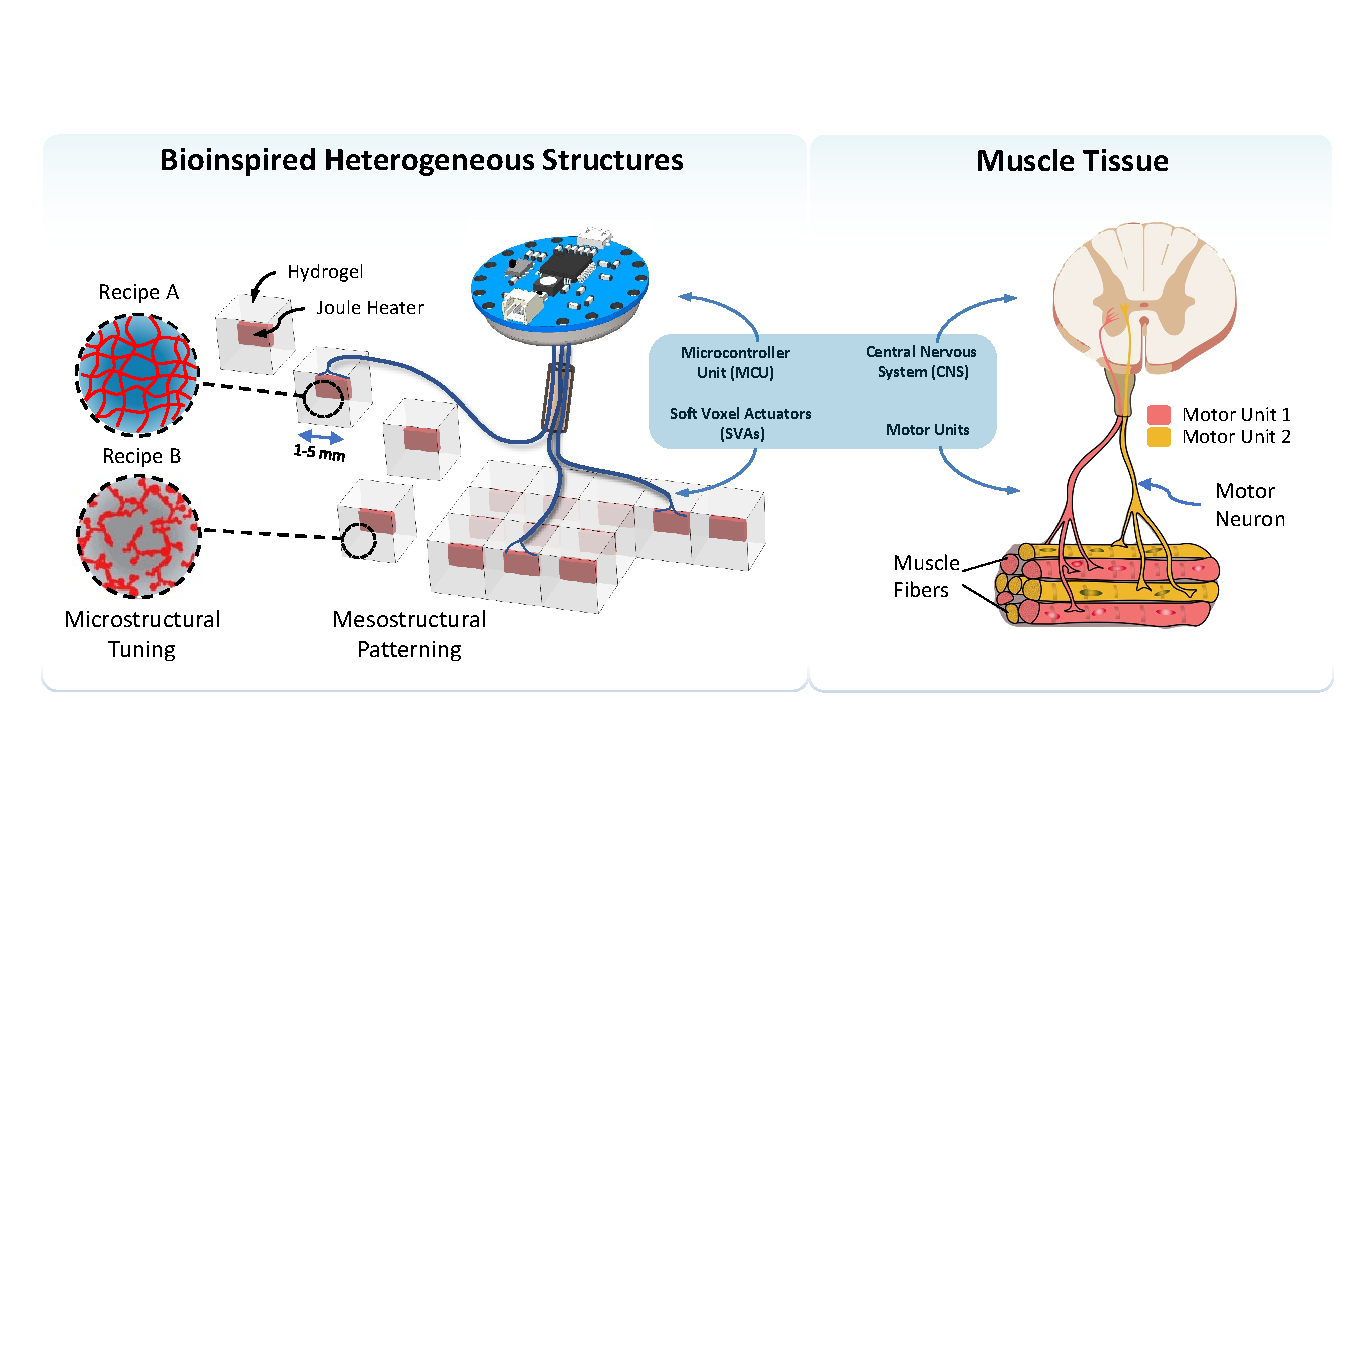
\includegraphics[width=\textwidth]{analogy.pdf}
\caption[Analogy between biology and artificial systems]{Illustration of bioinspired heterogeneous hydrogel structures composed of tunable and addressable voxels. \textbf{(Left)} Soft Voxel Actuators (SVAs) are electrically addressable building blocks whose deformations can be controlled by a microcontroller unit (MCU). SVAs are analogous to motor units, consisting of a motor neuron and associated muscle fibers, which deform in response to electrical impulses from the CNS \textbf{(Right)}. The microstructure of the hydrogels used to make SVAs can be altered, resulting in tunable material properties.}
\label{fig:analogy}
\end{figure}

\section{Concept}
Two types of SVAs have been realized and are described herein: one without an embedded heater (referred to as SVA-I), and one with an embedded heater (referred to as SVA-II), as shown in \figref{fig:heterogeneous}. 
% Though voxels of different shapes can be fabricated, the voxels in this paper are fabricated in the shape of basic rectangular blocks of varying sizes to simplify manufacturing, characterization, and assembly. 
% The \subfigref{fig:1}{b} shows the schematic of SVA-II 
% % as well as its physical realization 
% in two different states as the embedded heater is turned on and off. 
Various combinations of SVA-I and SVA-II can be used for designing and fabricating heterogeneous assemblies. 
% Standard sizes allow SVA-I and SVA-II units to be assembled into heterogeneous structures for the purposes of creating complex and controllable spatiotemporal motion. 
One possible combination, shown in \subfigref{fig:heterogeneous}{(i)}, uses SVA-I to create pre-programmed voxel assemblies. Based on the specific arrangement of SVA-I consisting of different swelling properties (mainly volume change ratio and rate), complex deformations can be demonstrated. These SVA assemblies deform in response to regular and repeated homogeneous temperature changes (such as the bulk heating and cooling of a water reservoir), generating motions without the need for an on-board energy source. It should be noted that hydrogels expand and contract based on the diffusion of water into and out of their structure when the temperature is passed their critical transition temperature which is around 32\textsuperscript{o} C in case of PNIPAAm hydrogels. Therefore, all our experiments are performed in a water bath. Another combination of SVAs shown in \subfigref{fig:heterogeneous}{(ii)}, uses thick film surface mount (SMD) resistive elements with a resistance of 10 ohms as Joule heaters in SVA-II units to create time-varying and inhomogeneous temperature fields, resulting in on-demand dynamic deformations and real-time reconfigurability. Details of the Joule heater elements are presented in the Supporting Information.\\ 
% This method is advantageous in applications where bulk temperature changes are infeasible.
% \note{tighten}. 

% irrespective of the environmental conditions. \note{NOT IF IT'S TOO HOT}
% \subfigref{fig:1}{d} shows the analogies between the biological muscle fibers and SVAs as addressable building blocks.

\begin{figure}[!ht]
\centering
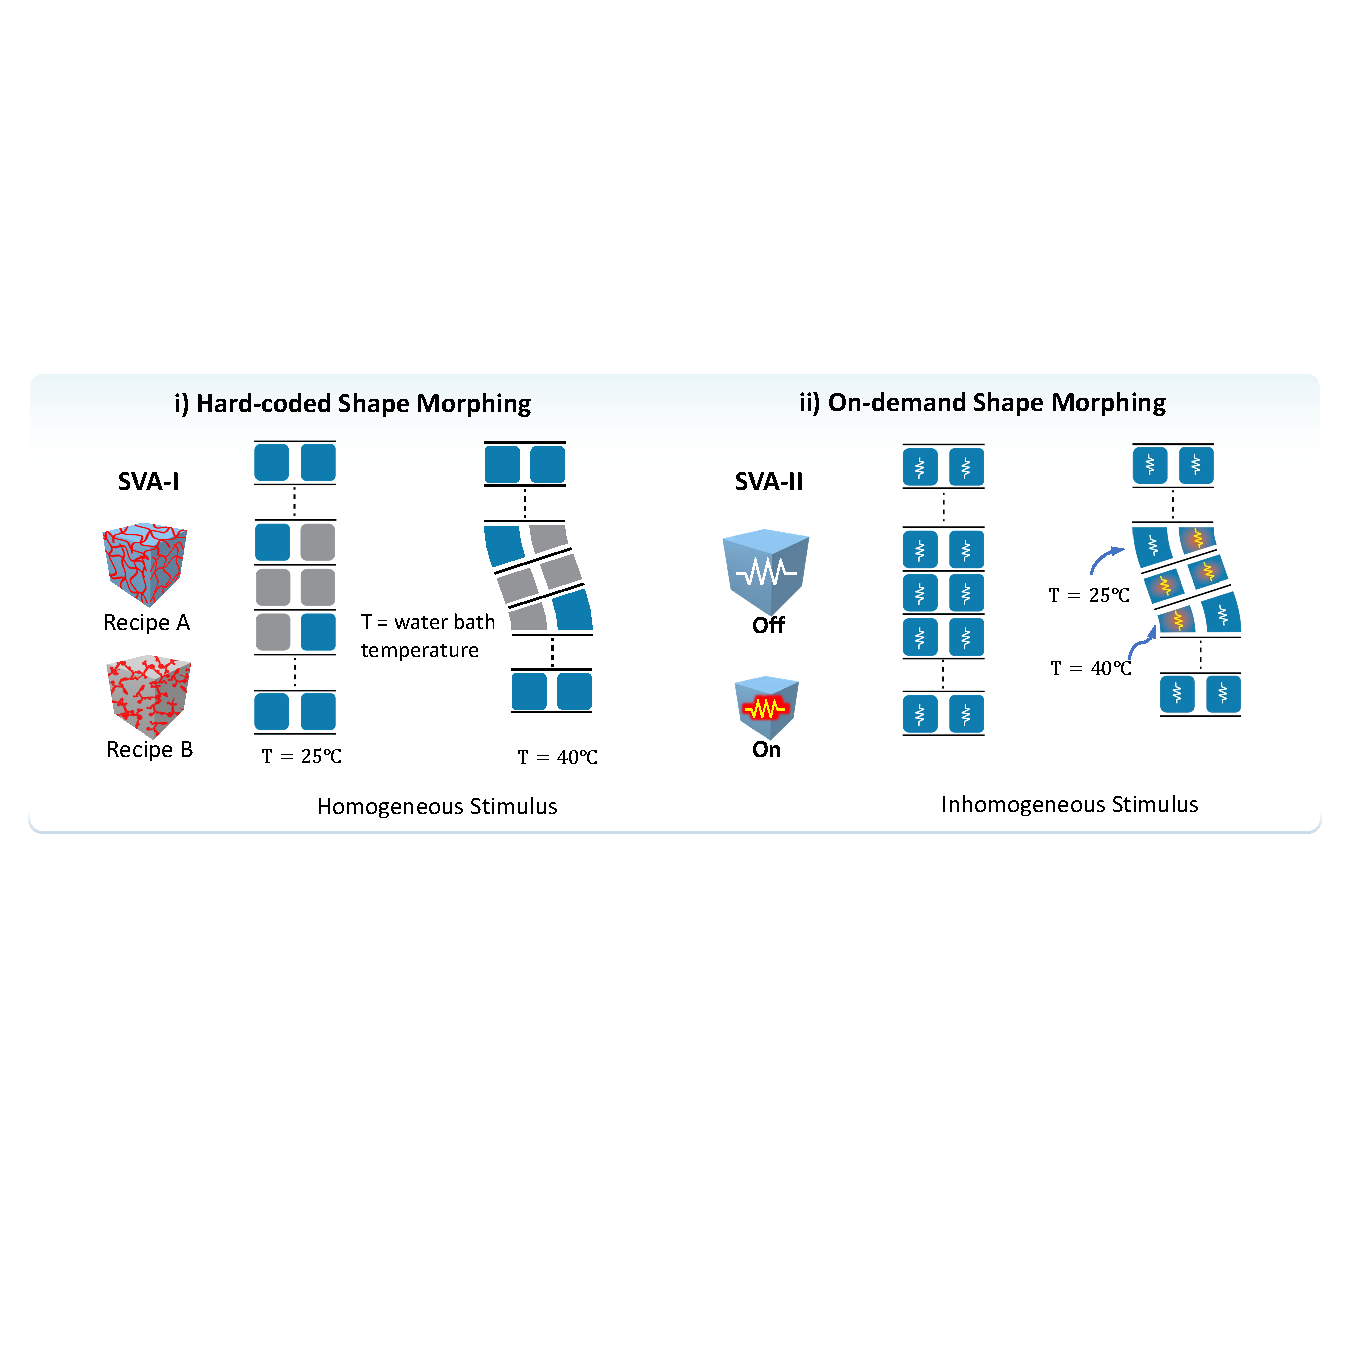
\includegraphics[width=\textwidth]{heterogeneous.pdf}
\caption[Illustration of bioinspired heterogeneous hydrogel structures]{Bioinspired heterogeneous hydrogel structures composed of tunable and addressable voxels. \textbf{i)} SVAs without embedded Joule heaters (SVA-I) are used to create structures with hard-coded shape morphing that respond to a homogeneous temperature field acting globally on the entire structure through the surrounding water bath. \textbf{ii)} SVAs with embedded heaters (SVA-II) are used to create structures with on-demand shape morphing by forming an inhomogeneous temperature field throughout the structure.}
\label{fig:heterogeneous}
\end{figure}

% achieved through altering the microstructure of the hydrogels,
% \note{Tuning the properties is made possible by a hydrogel recipe that supports generating materials with vastly different material properties with only slight differences in the fabrication steps.}
% \xh{I re-structured this paragraph by introducing the needs for a tunable synthesis method, following by a brief overview of current methods, before proposing our method.}
\section{Hydrogel Synthesis}
The ability to select from a broad range of material properties for SVA fabrication can expand the design space of resulting heterogeneous structures. Therefore, a synthesis method that can tune the ratio and rate of hydrogel volume change is required. 
% to achieve \sout{hydrogels with} a broad spectrum of swelling properties for creating modular SVA assemblies with efficient motion and dexterity.} 
A variety of physical and chemical methods have been explored to alter the swelling properties of hydrogels \cite{Zhang2008,Imran2010}. 
These methods are limited by factors such as the narrow range of achievable swelling properties \cite{Kim2016a,Gan2001}, large trade-offs in mechanical properties \cite{Li2018,Depa2012}, long processing times \cite{Zhou2018b, Ma2014}, and a need for careful control of synthesis conditions such as temperature \cite{Otsuka2012} and precursor additives \cite{Bodenberger2016}.\\ 

We take advantage of PNIPAAm's cononsolvency, a property of reduced solvation in a mixture of two solvents due to a delicate balance between polymer-solvent and solvent-solvent interactions \cite{Pica2016}. Employing a water and dimethyl sulfoxide (DMSO) mixed solvent in the PNIPAAm hydrogel precursor solution, followed by rapid photopolymerization to induce interconnected open pores, significantly enhanced the rate of water transport into and out of the hydrogel matrix and thus the actuation speed. The microstructure of the gel is altered by changing the water volume fraction (\(\varphi_{w}\)) in the mixed water/DMSO solvent. The SVA swelling rate and displacement, which are directly related to its hydrogel microstructure, are therefore tuned by merely  adjusting \(\varphi_{w}\). Polymerization solvent composition is known to affect the swelling properties of the synthesized PNIPAAm hydrogels \citesuperscript{Wang2017e,Lee2000, Zhang2002,Feng2011,Tokuyama2008}. 
%Rapid actuation using hydrogels requires ultrafast swelling speeds; 
The combination of the mixed solvent method with a fast 15\,s photopolymerization step is critical for inducing and fixing local aggregations of polymer chains in place,
% \rk{aggregation of polymer chains(what does it mean)}
resulting in PNIPAAm hydrogels with open pore structures (\firstsubfigref{fig:photothermo}{A(i)}). Such open pore structures exhibit significantly enhanced rates of thermoresponsive volume change in both heating and cooling phases, compared to conventional hours-long mixed solvent thermopolymerization methods (control experiment), in which the precursors are constantly diffusing towards a homogeneous molecular equilibrium throughout the duration of the reaction, leading to a less interconnected pore structure with thicker pore walls (\subfigref{fig:photothermo}{A(ii)}).
In order to ensure a valid comparison, the recipe for a representative thermopolymerized control hydrogel was carefully tuned using the initiator concentration while leaving all other components of the precursor solution unchanged, choosing a reaction time such that the conversion and water content match those of the photopolymerized hydrogel (Supporting Information and Table S2). It is readily observed that with equivalent water content, reaction conversion, and reaction solvent composition, the thermopolymerized hydrogel deswells as fast as the photopolymerized hydrogel \subfigref{fig:photothermo}{B(i)} and the two reach nearly identical shrunken volumes (Figure S8, Supporting Information). However the reswelling speed of the thermopolymerized control sample is $\sim$25 times slower than the photopolymerized sample, which can be attributed to the lower observable tortuosity present in the photopolymerized sample \subfigref{fig:photothermo}{B(ii)}. The Young's Modulus of the thermopolymerized hydrogel is $\sim$10 times higher than that of the photopolymerized one (Figure S9, Supporting Information). \\

\begin{figure}[!ht]
\centering
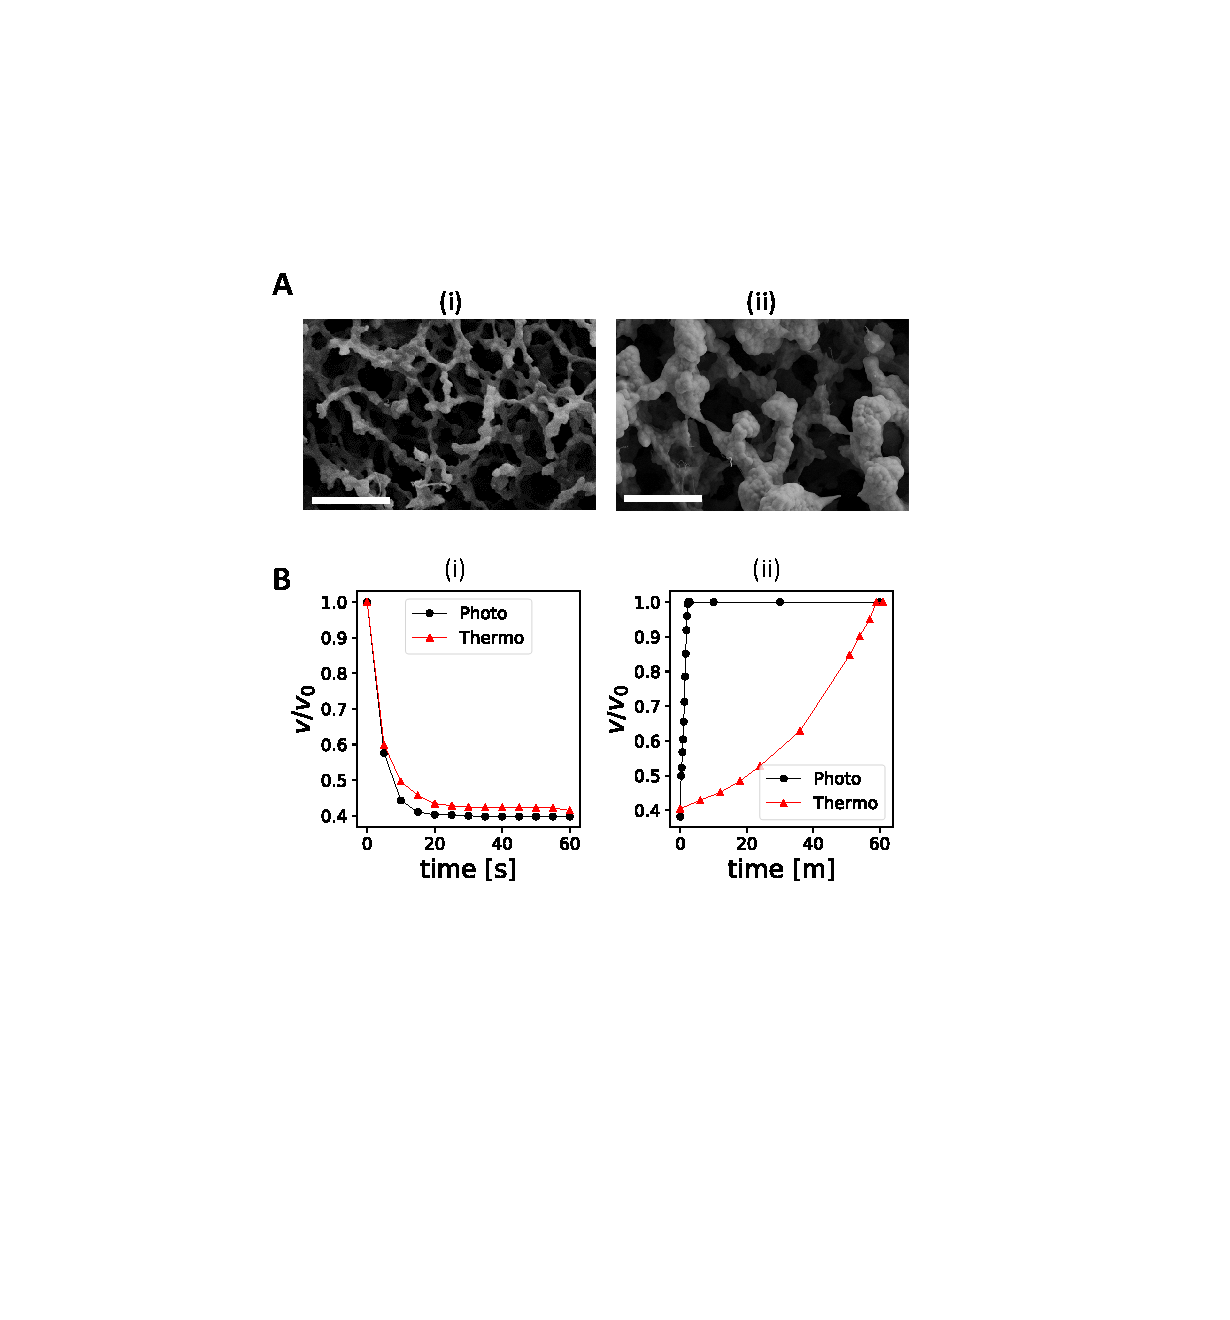
\includegraphics[width=0.85\textwidth]{photothermo.pdf}
\caption[Microstructure of thermopolymerized and photopolymerized gels ]{Comparison of photopolymerization and thermopolymerization methods on gel microstructure and performance.
% achieved by varying water volume fraction ($\varphi_w$) in the prepolymer mixture. 
\textbf{A)} SEM micrographs of photopolymerized (i) and thermopolymerized (ii) hydrogels synthesized in water volume fraction \(\varphi_{w}\)\,=\,0.27 (scale bar = $5\,\mu m$). \textbf{B)} Deswelling (i) and swelling (ii) rates of photopolymerized and thermopolymerized hydrogels synthesized in water volume fraction \(\varphi_{w}\)\,=\,0.27.}
% e) Compressive blocked force of a SVA-II f) Maximum compressive force as a function of $\varphi_w$ (extracted from e). 
% g) Young's modulus (E) as a function of SR. the data collection setup is described in methods.\note{change SR to $\varphi_w$}}
\label{fig:photothermo}
\end{figure}

The effect of varying \(\varphi_{w}\) on the hydrogel microstructure has been investigated by scanning electron microscopy (SEM), as shown in \firstfigref{fig:sem}. Six hydrogels consisting of various \(\varphi_{w}\) were synthesized; they are each represented by a character code ranging from HG00 (representing a hydrogel with \(\varphi_{w}\) = 0.0) to HG05 (representing a hydrogel with \(\varphi_{w}\) = 0.5). Details of the SEM imaging procedure are described in the Supporting Information. Distinct changes in the microstructure can be observed as a function of \(\varphi_{w}\), which impacts a variety of other material properties. When \(\varphi_{w}\) is increased from 0.0 to 0.2, pore size decreases and the pore wall surface begins to change from smooth to rough. We define \(\varphi_{w}\) = 0.2 as a critical water volume fraction, at which the microstructure of the gel starts to change from a closed-pore to an open-pore structure. SEM images for other values of \(\varphi_{w}\) are presented in Figure S4 in the Supporting Information.

\begin{figure}[!ht]
\centering
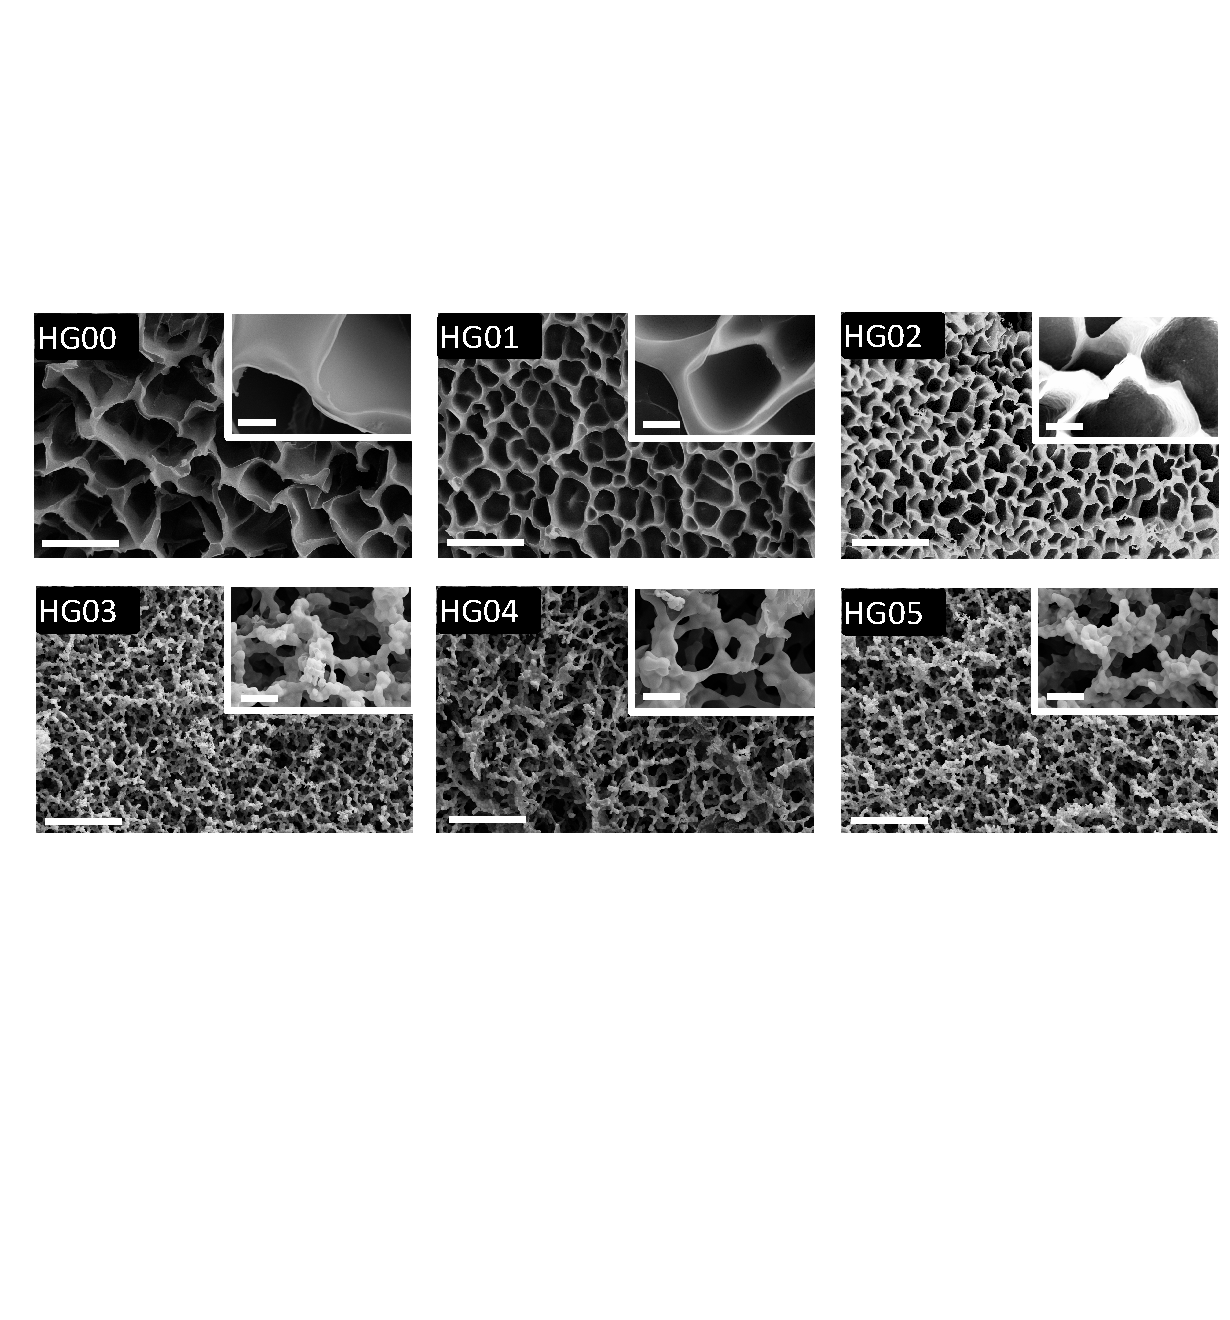
\includegraphics[width=\textwidth]{sem.pdf}
\caption[The effect of $\varphi_w$ on pore structure]{Tunable material properties using mixed solvent photopolymerization.
% achieved by varying water volume fraction ($\varphi_w$) in the prepolymer mixture. 
SEM images showing the effect of $\varphi_w$ on pore structure of the photopolymerized PNIPAAm hydrogel (scale bars $10\,\mu m$ and $1\,\mu m$ for low and high magnification, respectively).}
% e) Compressive blocked force of a SVA-II f) Maximum compressive force as a function of $\varphi_w$ (extracted from e). 
% g) Young's modulus (E) as a function of SR. the data collection setup is described in methods.\note{change SR to $\varphi_w$}}
\label{fig:sem}
\end{figure}

% \rk{this section should be rewritten to account for the fact that we have characterized actuators and not the material}
The changes in hydrogel microstructure play a role in the dynamic response of SVAs. The linear displacement generated by a SVA unit
% defined as the volume of the fully swollen SVA to that of dry gel -- 
is measured using a vision-based test setup as described and shown in the Supporting Information and Figure S3. \firstsubfigref{fig:forcedisp}{A} plots the time evolution of the displacement ($D$) of SVA units with different values of $\varphi_w$ 
%as a function of time -- 
as each SVA's embedded heater is turned on for 60\,s 
% \rk{should a space be inserted between the s 60?} \xh{typically yes, between the number and unit} 
and then turned off for 60\,s. The displacement over time of the hydrogel made with \(\varphi_{w}\) = 0.0 is included as the basis for comparison across all tests. The negative displacement observed is because the SVAs initially expand instead of contract as the heater is turned on which might be due to water slightly expanding and vaporizing. Two performance criteria for the SVA units, deformation rate ($DR$) and maximum displacement ($MD$), are extracted from the data in \subfigref{fig:forcedisp}{A} and are shown in \subfigref{fig:forcedisp}{B,C} respectively. During both heating and cooling, $DR$ is small for \(\varphi_{w} < 0.2\). At \(\varphi_{w} = 0.2\), the $DR$ during heating is more than 36 times the $DR$ during cooling. As a result, fast and large deformations are observed during the 60\,s of heating, and almost no deformation is observed during the 60\,s of cooling. 
Highest $DR$ (in both heating and cooling) occurs in gels with $\varphi_w = 0.3$, while $MD$ peaks at $\varphi_w = 0.2$ and decrease thereafter.
% \note{more, or faster? rate or total shrinkage? use quantitative DR, MD etc..} 
% as the heater is turned on. When the heater is turned off, however, the gel does not swell during the 60s duration of the experiment.
In addition to swelling properties, other mechanical properties such as Young's modulus and force produced by the SVAs can also be tuned by adjusting \(\varphi_{w}\) (Figure S5, Supporting Information).\\ 
\begin{figure}[!ht]
\centering
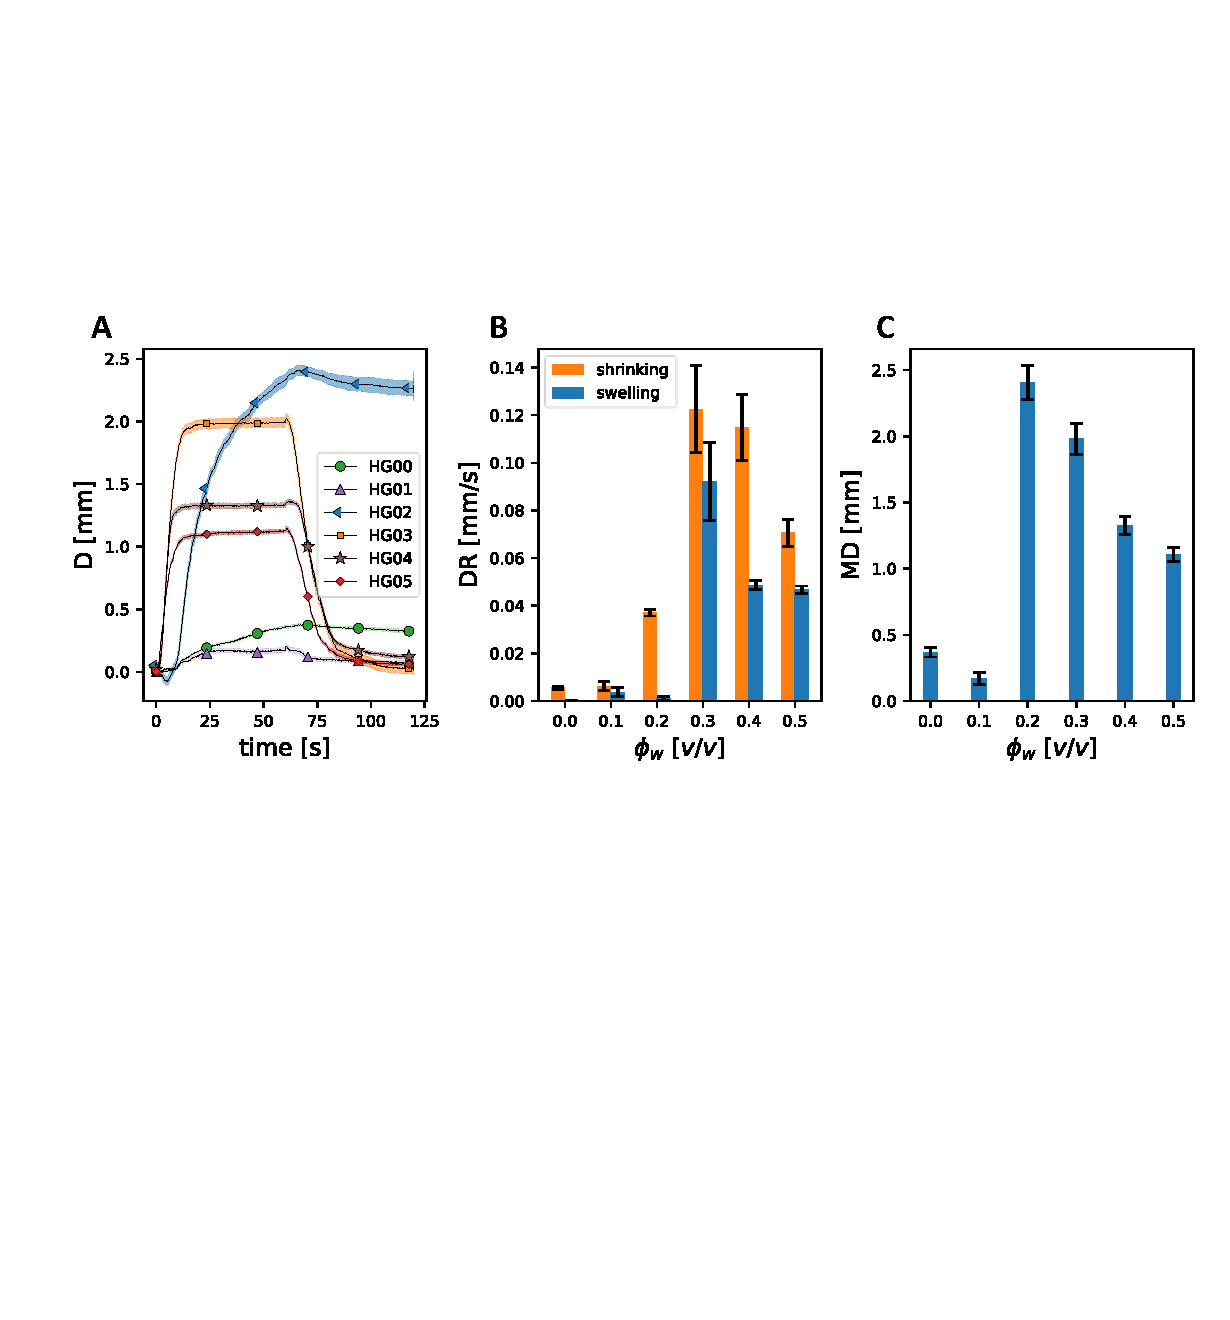
\includegraphics[width=\textwidth]{forcedisp.pdf}
\caption[The effect of $\varphi_w$ on mechanical properties]{Tunable material properties using mixed solvent photopolymerization.
% achieved by varying water volume fraction ($\varphi_w$) in the prepolymer mixture. 
\textbf{A)} Displacement (D) over time generated by SVA-II units with different values of \(\varphi_{w}\)  under a $1\,gf$ load, as measured by the setup described in the Supporting Information. \textbf{C,D)} Displacement rate (DR) and maximum displacement (MD) of SVA-II units as a function of $\varphi_w$,(extracted from A as described in the Supporting Information).}
% e) Compressive blocked force of a SVA-II f) Maximum compressive force as a function of $\varphi_w$ (extracted from e). 
% g) Young's modulus (E) as a function of SR. the data collection setup is described in methods.\note{change SR to $\varphi_w$}}
\label{fig:forcedisp}
\end{figure}

\section{Hard-coded Shape Morphing}
% We have used the tunable hydrogel recipe and voxel-based assembly as tools to increase the variety and complexity of shape transformations in heterogeneous structures. Due to the wide range of tunable properties enabled by our hydrogel synthesis technique,
A variety of heterogeneous structures can be produced that transform into different configurations, depending on their hard-coded material domains.
% \rk{add description about why we grouped voxels together and cast them together} 
As a first example, a beam with only two material domains is fabricated from HG00 and HG02 hydrogels (\firstsubfigref{fig:bilayer}{(i)}). 
% We use this structure as a bench mark to compare the performance of structures produced using our mixed solvent method to those presented in materials science literature\note{\citesuperscript{}}. 
At 20\,$^{\circ}$C, the beam is in its equilibrium position. As the temperature increases to 45\,$^{\circ}$C, the HG02 hydrogel shrinks more than HG00 (from \subfigref{fig:forcedisp}{B,C}, both $MD$ and $DR$ are higher for HG02), 
% \note{more or faster?} 
which results in a stress mismatch. To balance these stresses, the beam bends into a circular shape as seen in \subfigref{fig:bilayer}{(ii) ,(iii)}.
We will henceforth refer to this structure as a `gripper'. %for future reference. 
\begin{figure}[!ht]
\centering
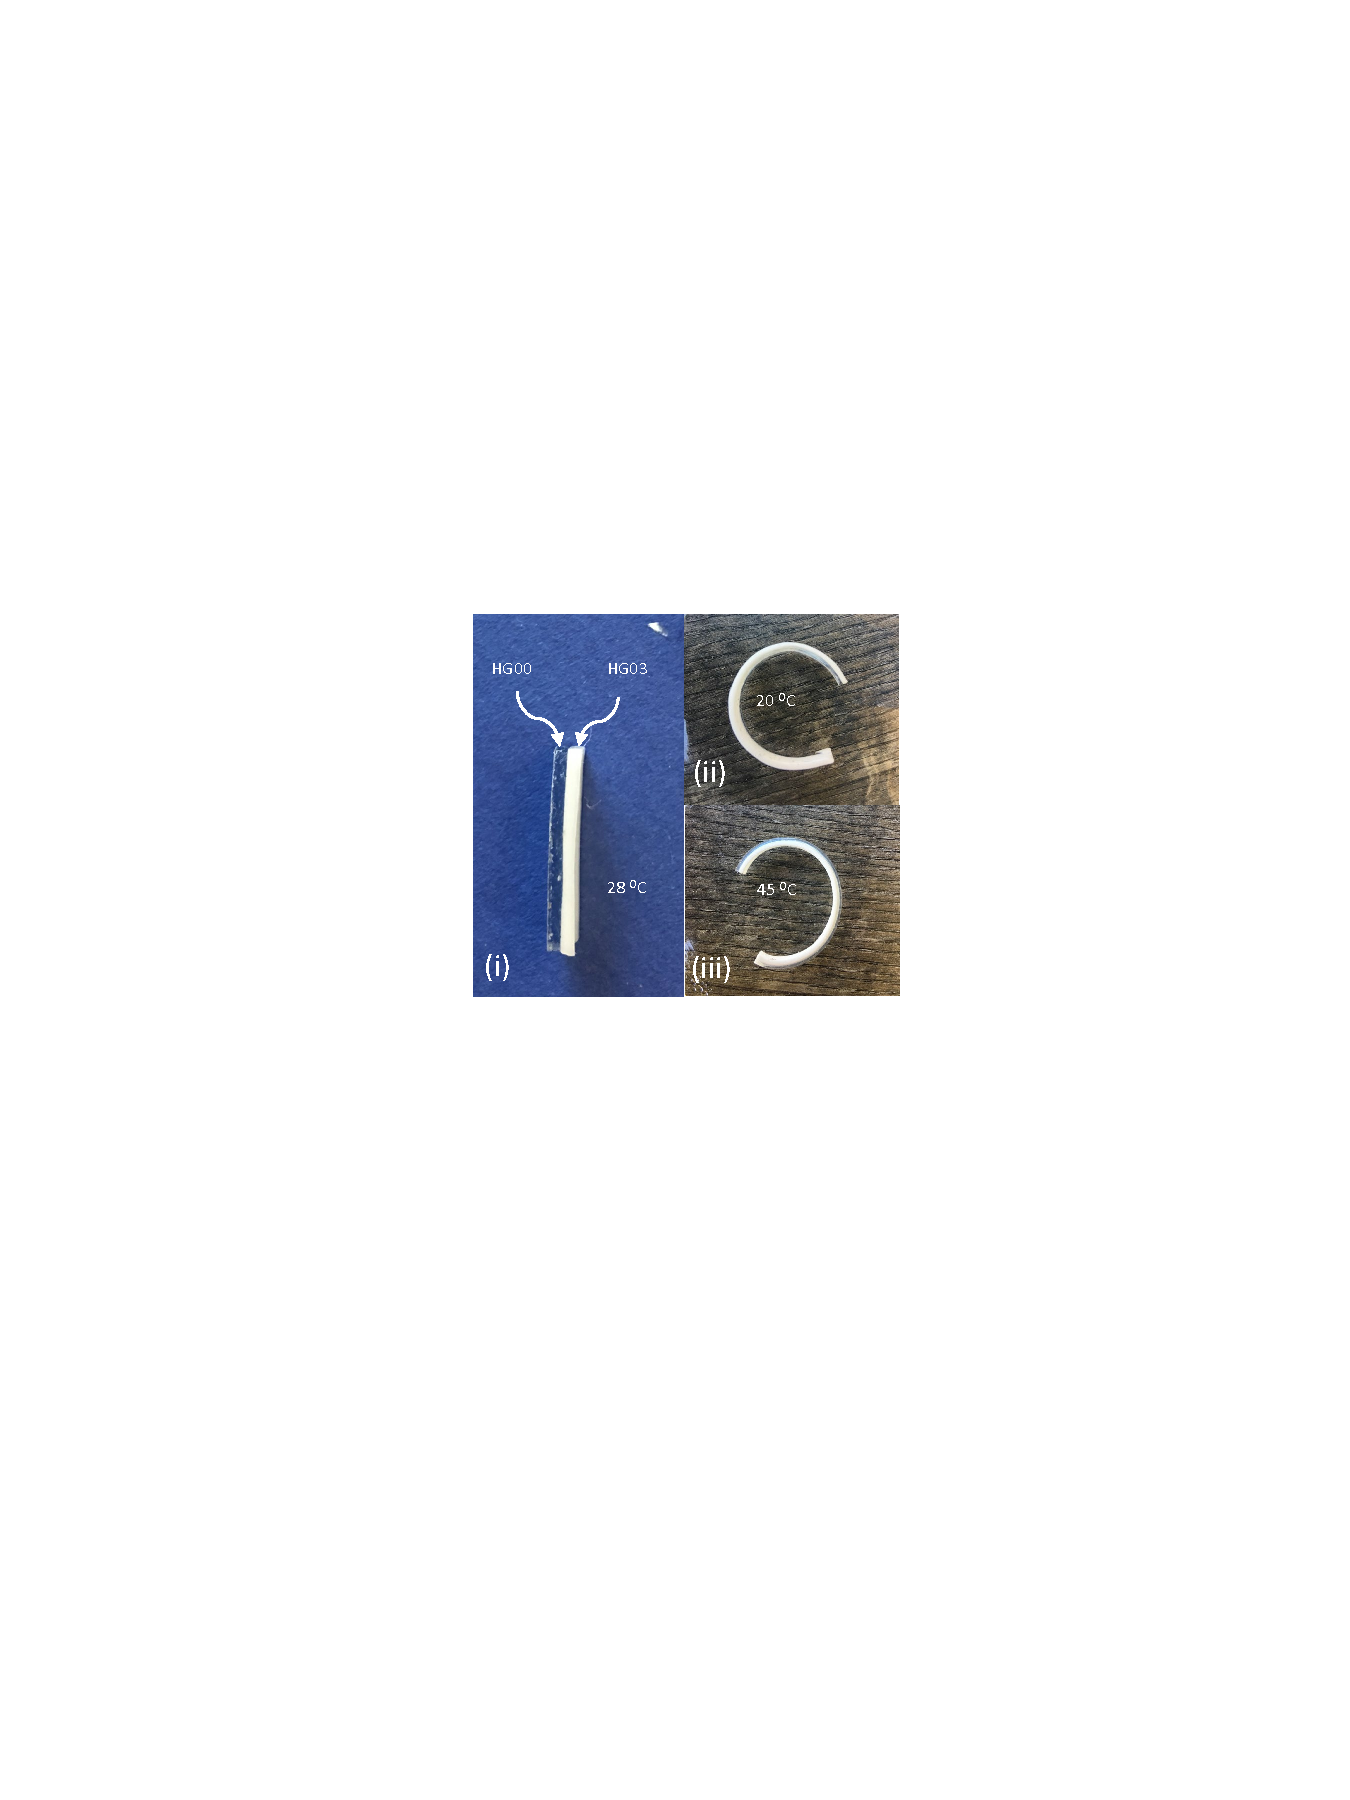
\includegraphics[width=0.6\textwidth]{bilayer.pdf}
\caption[Realization of structural inhomogeneity]{Realization of structural inhomogeneity through patterning of hydrogels with different swelling properties. \textbf{i)} A two-material, two-region structure made of HG00 and HG03 regions \textbf{ii,iii)} The bilayer structure can almost bend into a circle when the surrounding water bath temperature is raised above or below the transition temperature of PNIPAAm hydrogel (~32\,$^{\circ}$C)}
\label{fig:bilayer}
\end{figure}

A second example uses HG00 and HG02 hydrogels again, but this time with 
% a voxel-based arrangement, creating shape morphing structures with multiple 
8 material domains, as shown in \firstsubfigref{fig:hardcoded}{(i-iii)}. The beams in these figures consist of different arrangements of HG00 and HG02 voxels, and as a result exhibit different deformations when subjected to a homogeneous temperature change in the surrounding water from 20\,$^{\circ}$C to 45\,$^{\circ}$C (for details, see Movie S1 in the Supporting Information)\\
\begin{figure}[!ht]
\centering
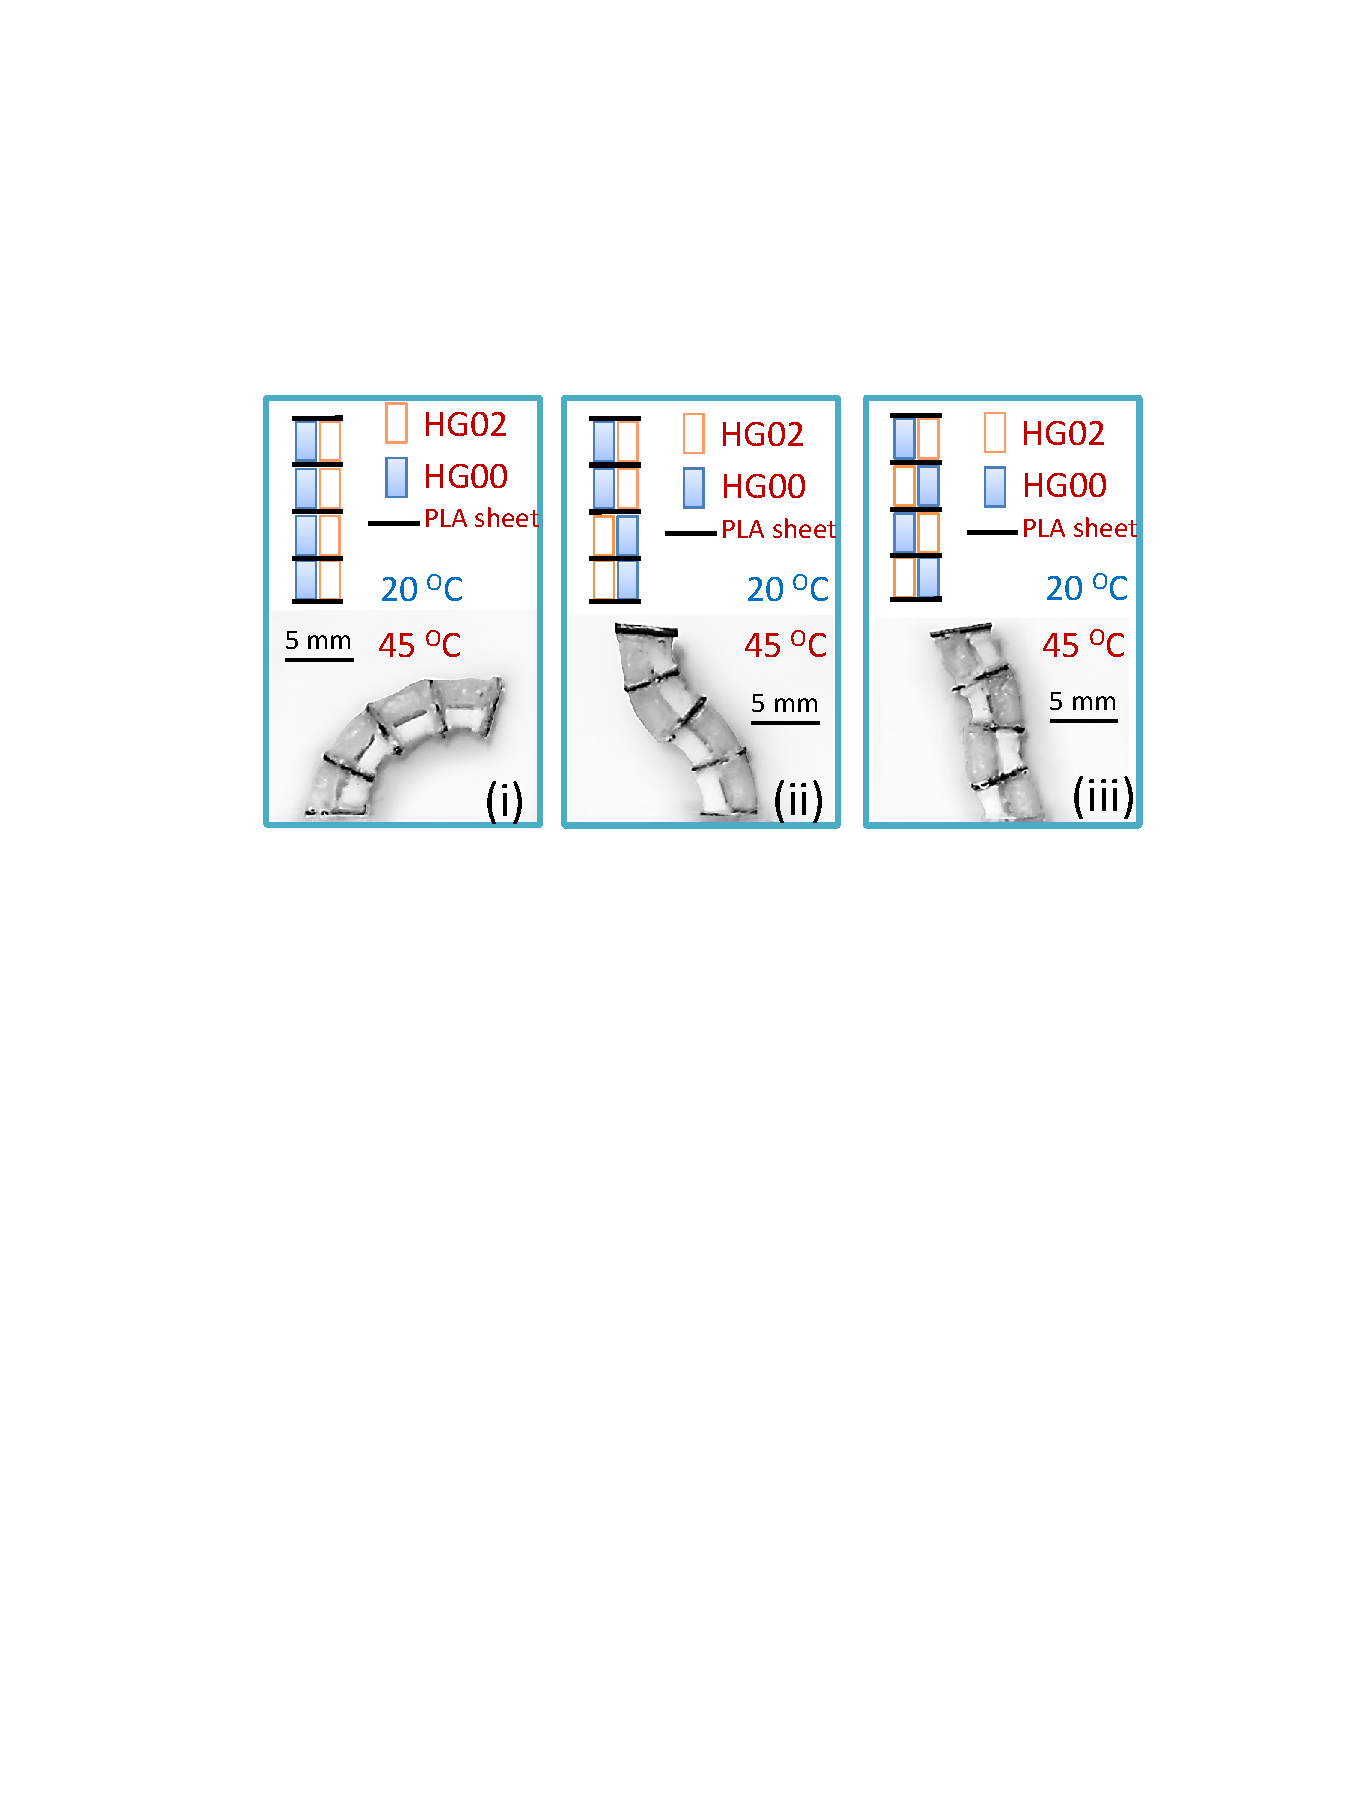
\includegraphics[width=0.8\textwidth]{hardcoded.pdf}
\caption[Using SVAs to increase deformation domains]{Realization of structural inhomogeneity through patterning of hydrogels with different swelling properties. \textbf{i-iii)} Increasing the number of material domains in the structure enables it to achieve more diverse shapes. When the surrounding water bath temperature is increased, each structure reconfigures into a different shape, depending on its arrangement of SVA-I units.}
\label{fig:hardcoded}
\end{figure}

Patterning material domains can be used to leverage the shape transformations into unique functions tied to structural heterogeneity. To demonstrate this \textit{structure--function} relationship, two different structures, Str-I and Str-II, are made with different combinations of HG00, HG02, and HG03, as shown in \firstfigref{fig:hardcodedrobot}. These structures represent a combination of the structures in \figref{fig:bilayer} and \figref{fig:hardcoded}. In response to a global cyclic temperature change from 20\,$^{\circ}$C to 45\,$^{\circ}$C and back to 20\,$^{\circ}$C, these structures are observed to bend towards an object, grasp it (by wrapping around it), and transport it to another location. 
\begin{figure}[!ht]
\centering
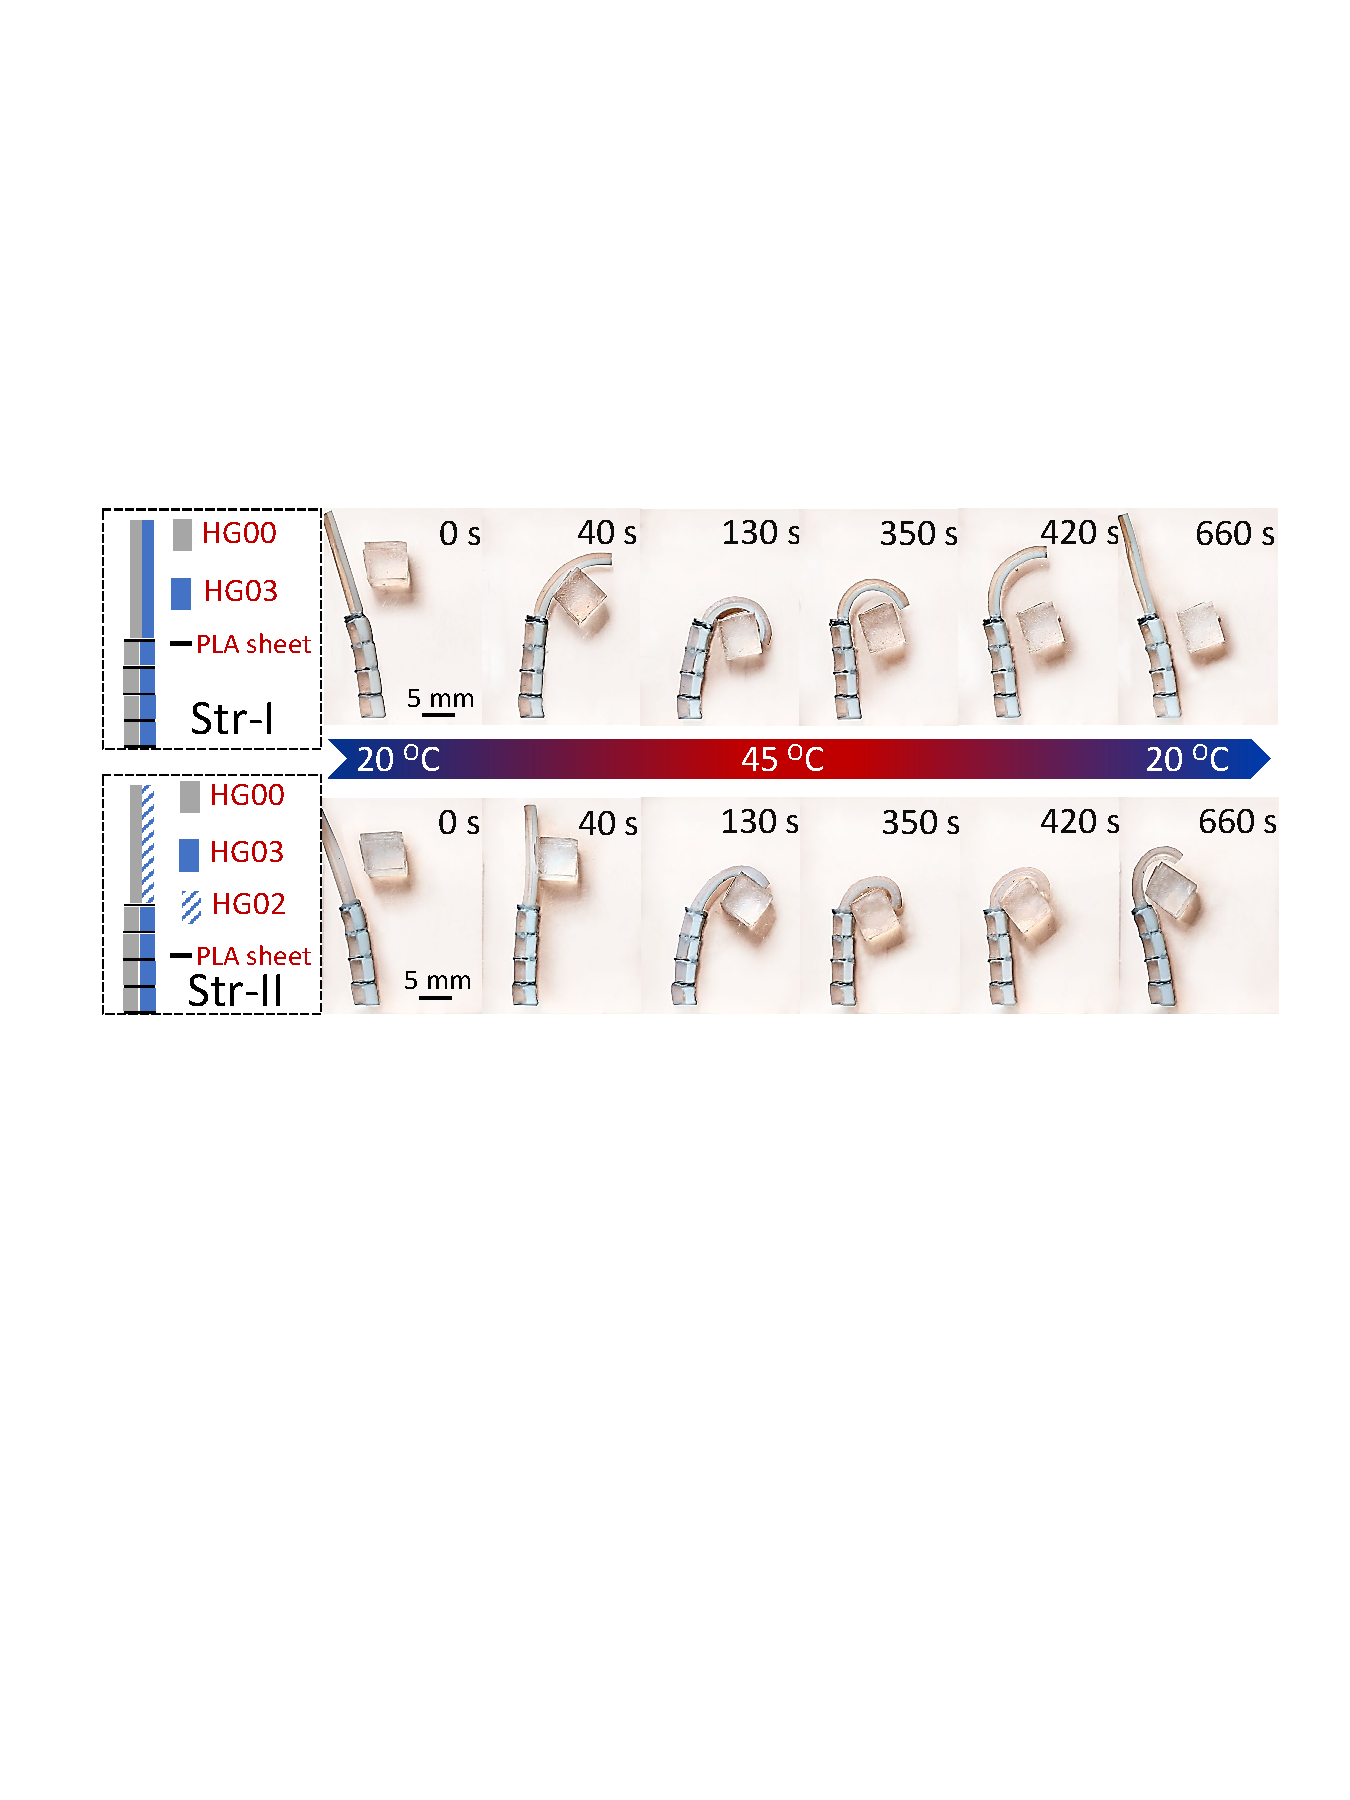
\includegraphics[width=\textwidth]{hardcodedrobot.pdf}
\caption[Object transport in hard-coded structures]{Realization of structural inhomogeneity through patterning of hydrogels with different swelling properties. Hybrid structures comprised of substructures with the SVA arrangements in \figref{fig:bilayer} and \figref{fig:hardcoded} are capable of manipulating objects. The material distribution in two example structures, denoted by Str-I and Str-II, is shown in the schematic on the far left. The snapshots display the configurations of the two structures over time as the global water bath temperature is increased and then decreased.}
\label{fig:hardcodedrobot}
\end{figure}

The geometric configuration of material domains in both structures are the same. However, the `gripper' portion of Str-I is a combination of HG00/HG03 domains, whereas in Str-II it is a combination of HG00/HG02 domains. As a result of this minor material difference, the object grasped by Str-I and Str-II moves along different trajectories, as seen in \firstfigref{fig:hardcodedtraj}{A}, despite an identical set of initial conditions. Due to the high $DR$ of HG03 during the cooling phase (\subfigref{fig:forcedisp}{B}), the gripper in Str-I opens and the object is released in the early stages of the cooling phase. The gripper in Str-II, on the other hand, does not open at the same time as Str-I and continues to hold the object throughout its cooling phase; this can be attributed to the lower $DR$ of the HG02 layer compared to HG03. To illustrate these differences, the $x$ and $y$ coordinates of the object over time are plotted in \subfigref{fig:hardcodedtraj}{B}, and the time when the object is released by each structure is indicated. Achieving inhomogeneous deformations in response to a homogeneous global stimulus using structures with hard-coded deformations as described simplifies the system and eliminates the need for on-board power sources.\\ 

\begin{figure}[!ht]
\centering
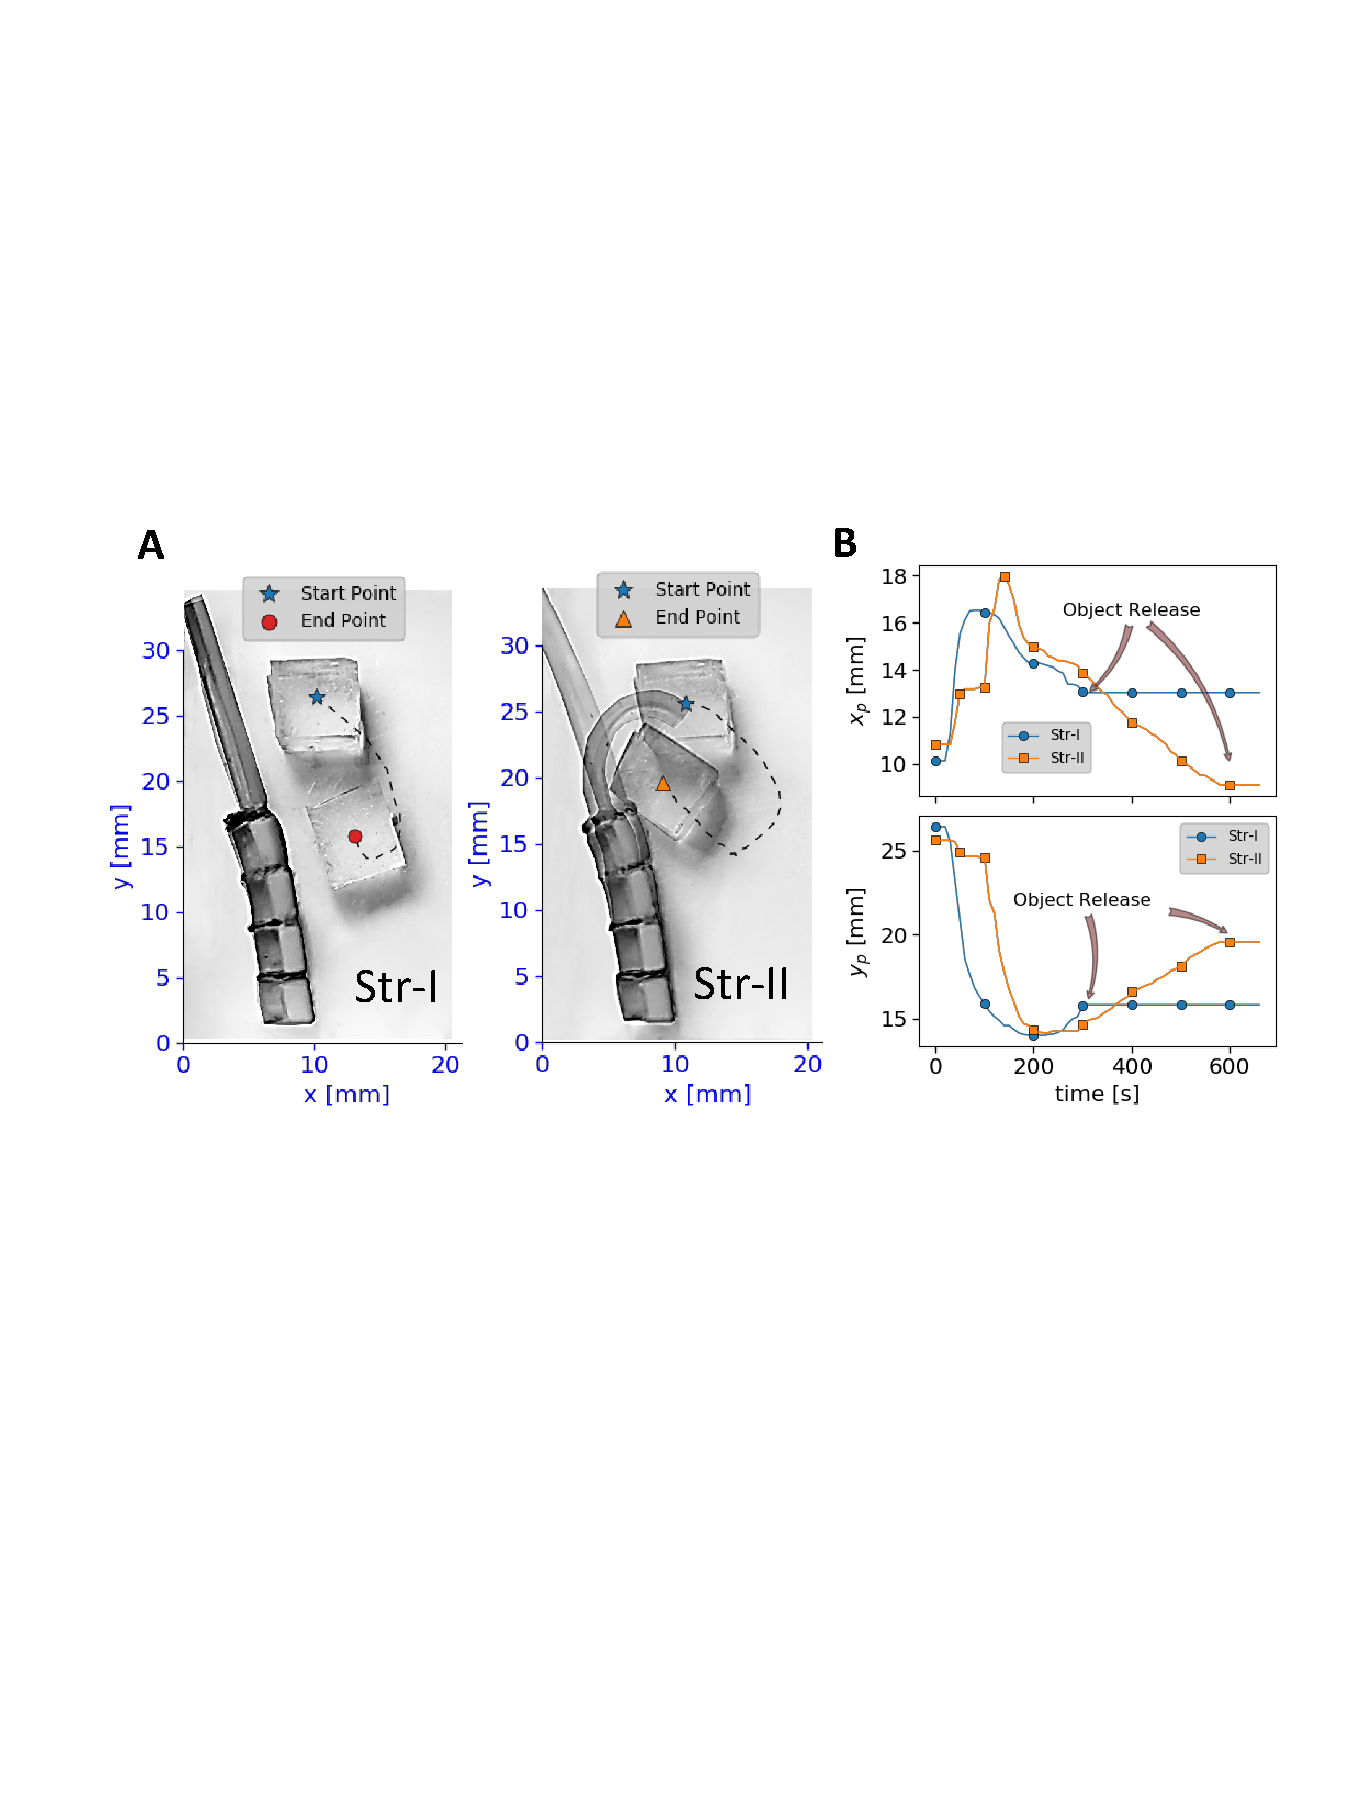
\includegraphics[width=\textwidth]{hardcodedtraj.pdf}
\caption[Trajectories created by hard-coded structures]{Realization of structural inhomogeneity through patterning of hydrogels with different swelling properties. \textbf{A)} Image showing the start position,  end position, and  trajectory of the  object manipulated by Str-I (left) and Str-II (right). \textbf{B)} Time evolution of the $x$ and $y$ coordinates of the manipulated object's center of mass.  Str-I releases the object   a $t=300$ s, while  Str-II releases it at $t= 600$ s, demonstrating the versatility of the voxel-based assembly approach to creating heterogeneous structures with diverse functions.}
\label{fig:hardcodedtraj}
\end{figure}

\section{On-demand Shape Morphing}
For applications in dynamic, unstructured environments, such as underwater robotic exploration, it is less useful to pre-program complex trajectories into a structure, since global stimulus control is not always feasible. To enable on-demand thermoresponsive shape morphing in these conditions, SVA-II units may be employed, as depicted in \subfigref{fig:heterogeneous}{(ii)}. The 40×11×5 mm structure shown in \firstsubfigref{fig:16svaArm}{A} was assembled using 16 SVA-II units. These SVAs are made of HG03, which exhibits the highest $DR$ observed across all recipes (\subfigref{fig:forcedisp}{B}). The first example of on-demand shape morphing is illustrated in \subfigref{fig:16svaArm}{B(i)}, in which the structure morphs into an `S' shape and a `reverse S' shape when particular SVAs are actuated via commands from a microcontroller. %where the same structure morphs into `S' and `reverse S' shapes based on commands from a microcontroller. 
A second example of on-demand shape morphing is illustrated in \subfigref{fig:16svaArm}{B(ii)}; it highlights how the curvature of a structure may be varied as a function of the voltage supplied to the SVA-II units.\\


\begin{figure}[!ht]
\centering
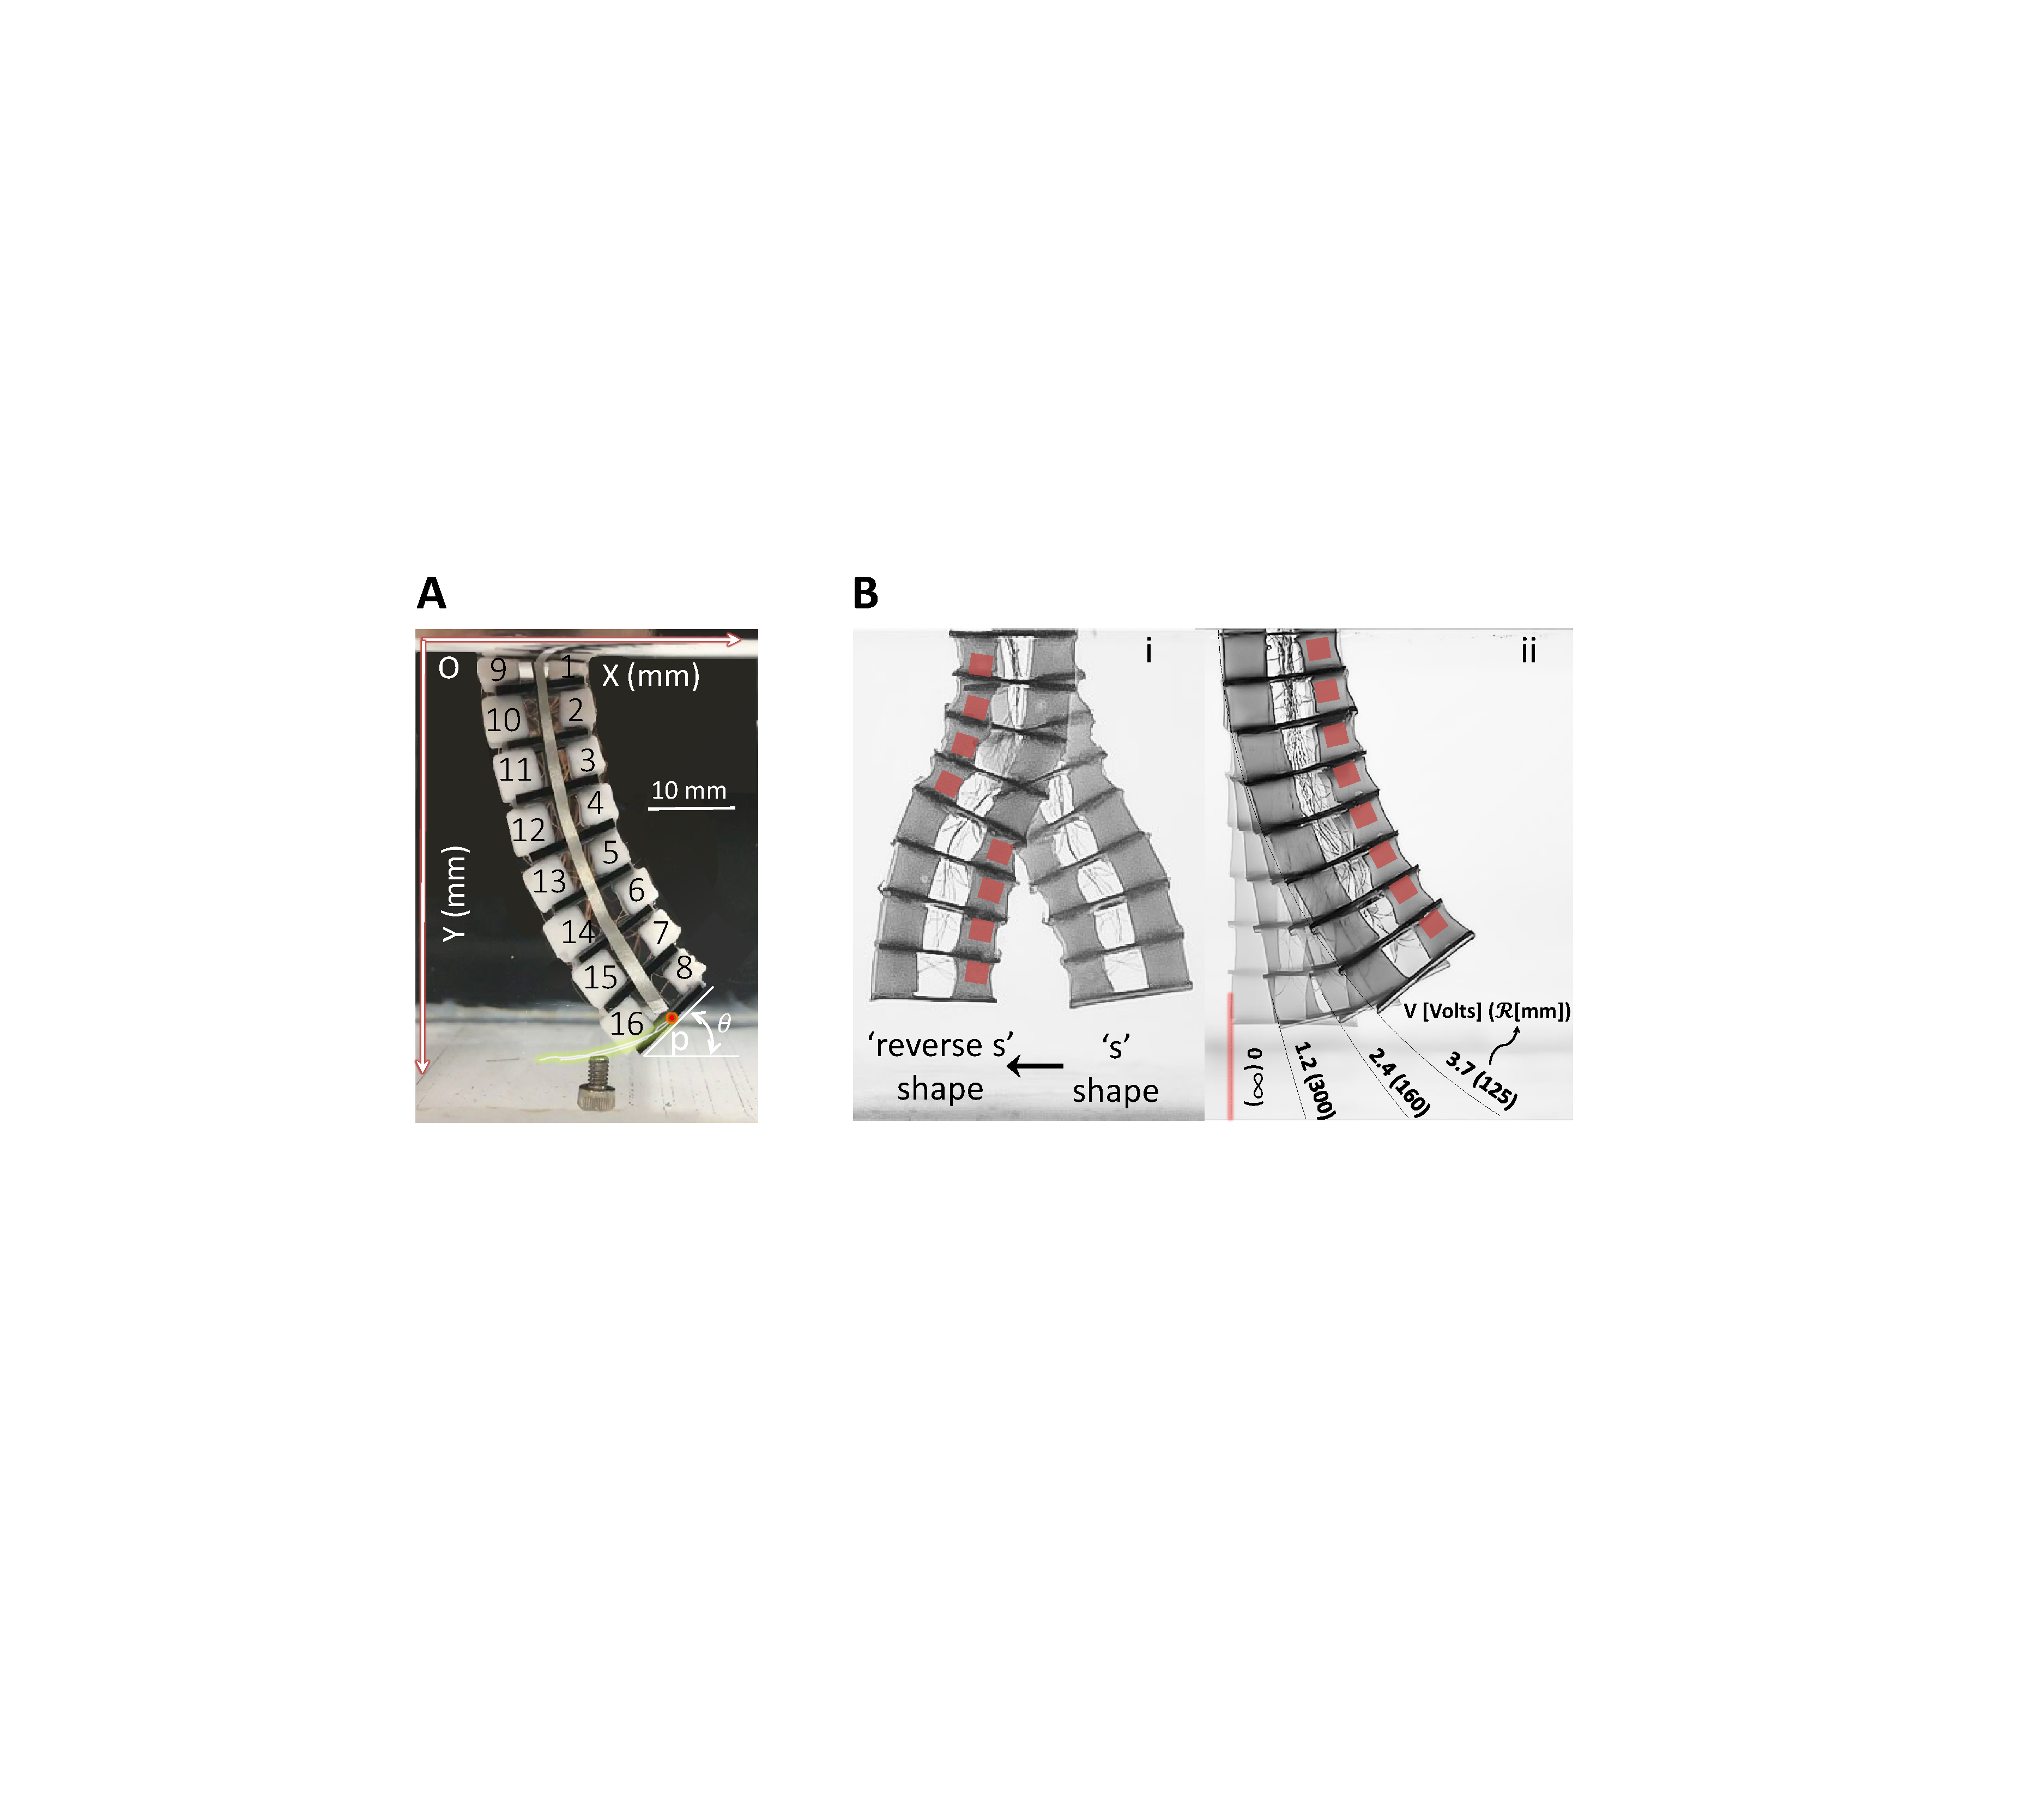
\includegraphics[width=\textwidth]{16svaArm.pdf}
\caption[A miniature soft robot consisting of 16 addressable SVA-II units]{A miniature heterogeneous structure consisting of 16 addressable SVA-II units. \textbf{A)} SVA numbering scheme and the coordinate system used to measure the position of the point $p$ and the angle $\theta$ of the end plate. \textbf{B)} On-demand shape morphing of the structure. i) The structure morphs from an `S' shape to a `reverse S' shape when particular SVAs are activated. ii) The structure's radius of curvature ($\mathcal{R}$) depends on the activation voltage ($V$) applied to SVAs 1-8.}
\label{fig:16svaArm}
\end{figure}

Moving from static to dynamic on-demand shape changes requires time-varying activation of SVAs.
As demonstrated in \firstfigref{fig:armTrajOnOff}, the choice of SVA actuation pattern can influence the end-effector trajectory of a structure. In this experiment, SVAs 1 thorough 8 are activated according to patterns denoted by P1 and P2. Each SVA is activated with maximum voltage (3.7\,V) for 15\,s before the next SVA is activated.
\begin{figure}[!ht]
\centering
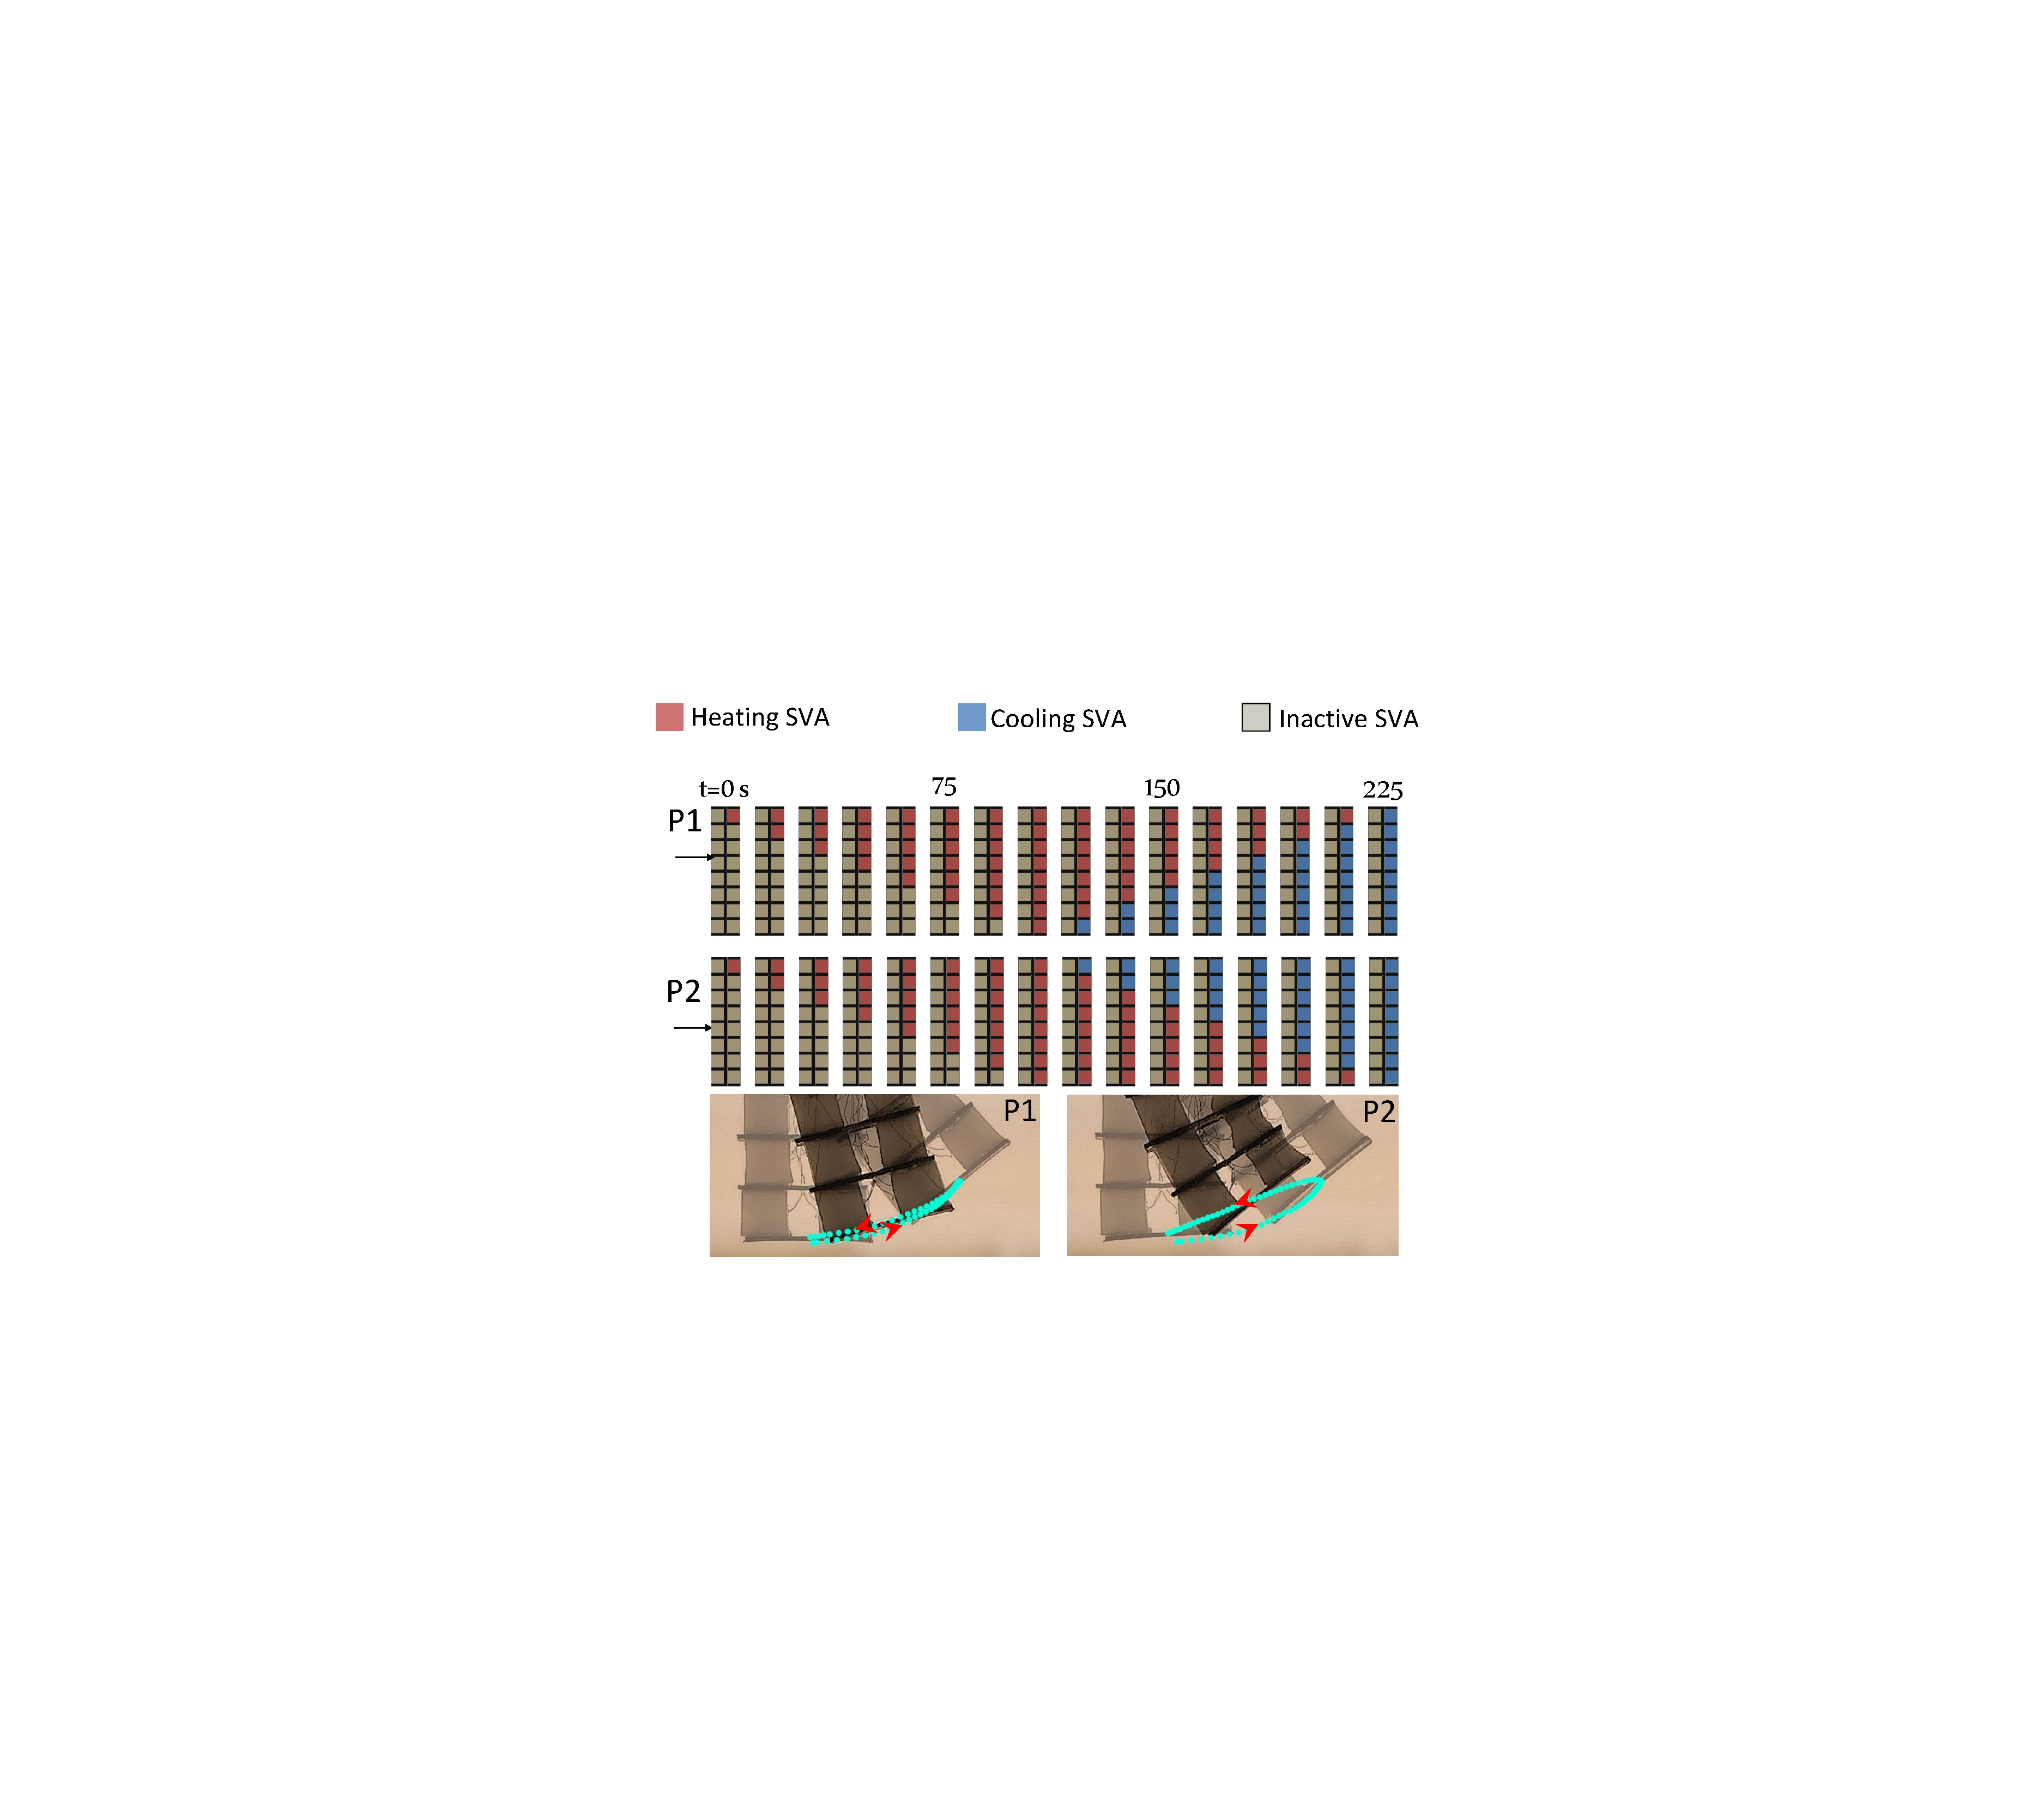
\includegraphics[width=0.8\textwidth]{armTrajOnOff.pdf}
\caption[Dynamic shape changes by On/Off signals]{Dynamic shape changes are implemented by sequentially activating SVAs. In this case, SVAs 1 through 8 are activated according to the patterns labeled P1 and P2. The trajectory followed by the tip of the structure (shown at the bottom) can thus be adjusted on-demand. For details, see Movie S6 in the Supporting Information.}
\label{fig:armTrajOnOff}
\end{figure}

While complex motion of SVA-II-based structures may be achieved using simple on (3.7\,V) and off (0\,V) activation signals, as discussed, intermediate voltages may also be applied to further enhance the complexity of shape change in soft heterogeneous structures. To demonstrate this, phase-shifted sinusoidal voltages were used as activation signals to generate longitudinal traveling waves in the structure. A pair of SVAs (comprising a SVA on the left and its adjacent SVA on the right) are activated using the same sinusoidal signal; SVAs 4 and 12 were not activated, to serve as a geometric reference point. The sinusoidal voltages applied to every SVA pair were $\frac{\pi}{8}~rad$ out of phase with the voltages applied to its nearest active SVA pair. As an example, sinusoidal signals for four SVA pairs are shown in  \firstfigref{fig:sineWaves}. A contraction wave was formed as a result of this input signal pattern and traveled along the length of the structure, as illustrated in \firstfigref{fig:4peristaltic}. Movie S4 in the Supporting Information shows in detail how these waves are generated and propagated along the structure. Every point on the structure oscillates in a sinusoidal manner as the wave passes through it. The midpoint of the inactive SVA pair, which is highlighted by a yellow square in \figref{fig:peristaltic}, is shown as a reference point on the structure. Additionally, by sending the sinusoidal signals to SVAs located on only one side of the structure, for example SVAs 1 through 8, transverse traveling waves were generated in the structure (Movie S4, Supporting Information).

\begin{figure}[!ht]
\centering
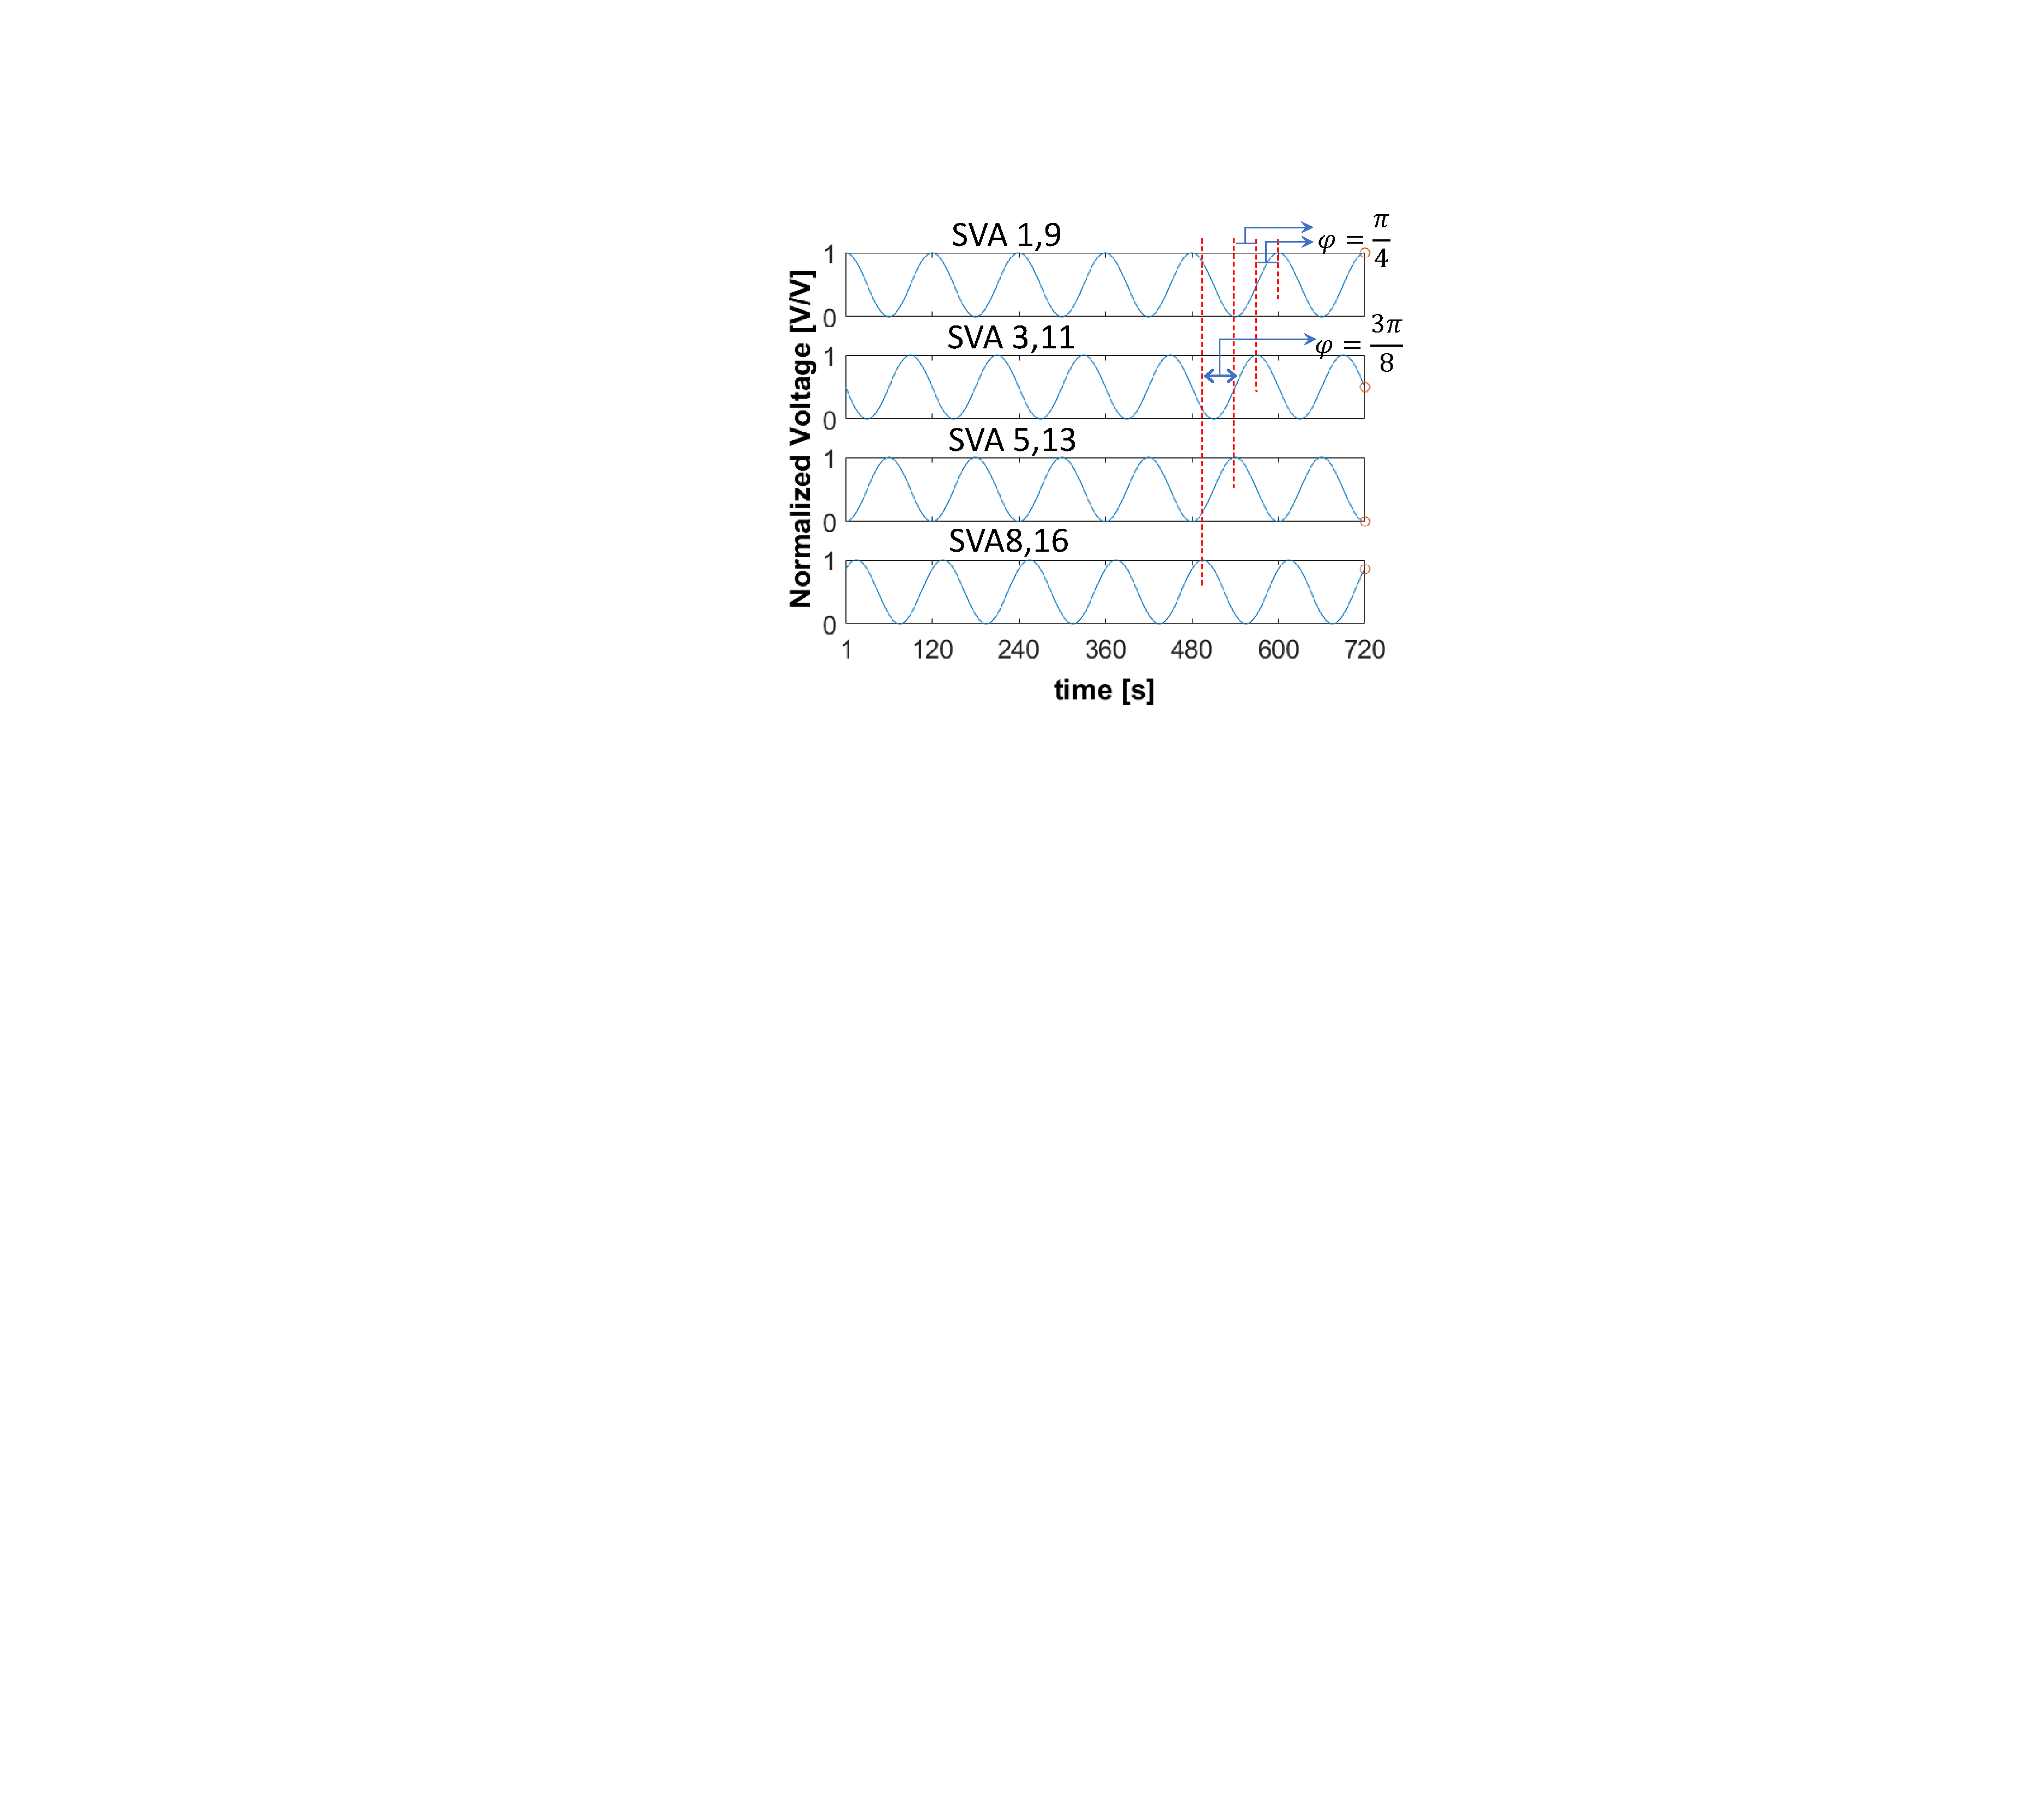
\includegraphics[width=0.7\textwidth]{sineWaves.pdf}
\caption[Normalized sinusoidal voltages]{Normalized sinusoidal voltages used to create longitudinal traveling waves in the structure. The voltages applied to 8 of the 16 SVAs are shown here. The SVAs are activated in pairs, and the voltage applied to each SVA pair is $\frac{\pi}{8}~rad$ out of phase with respect to the voltage applied to the next active pair.}
\label{fig:sineWaves}
\end{figure}

\begin{figure}[!ht]
\centering
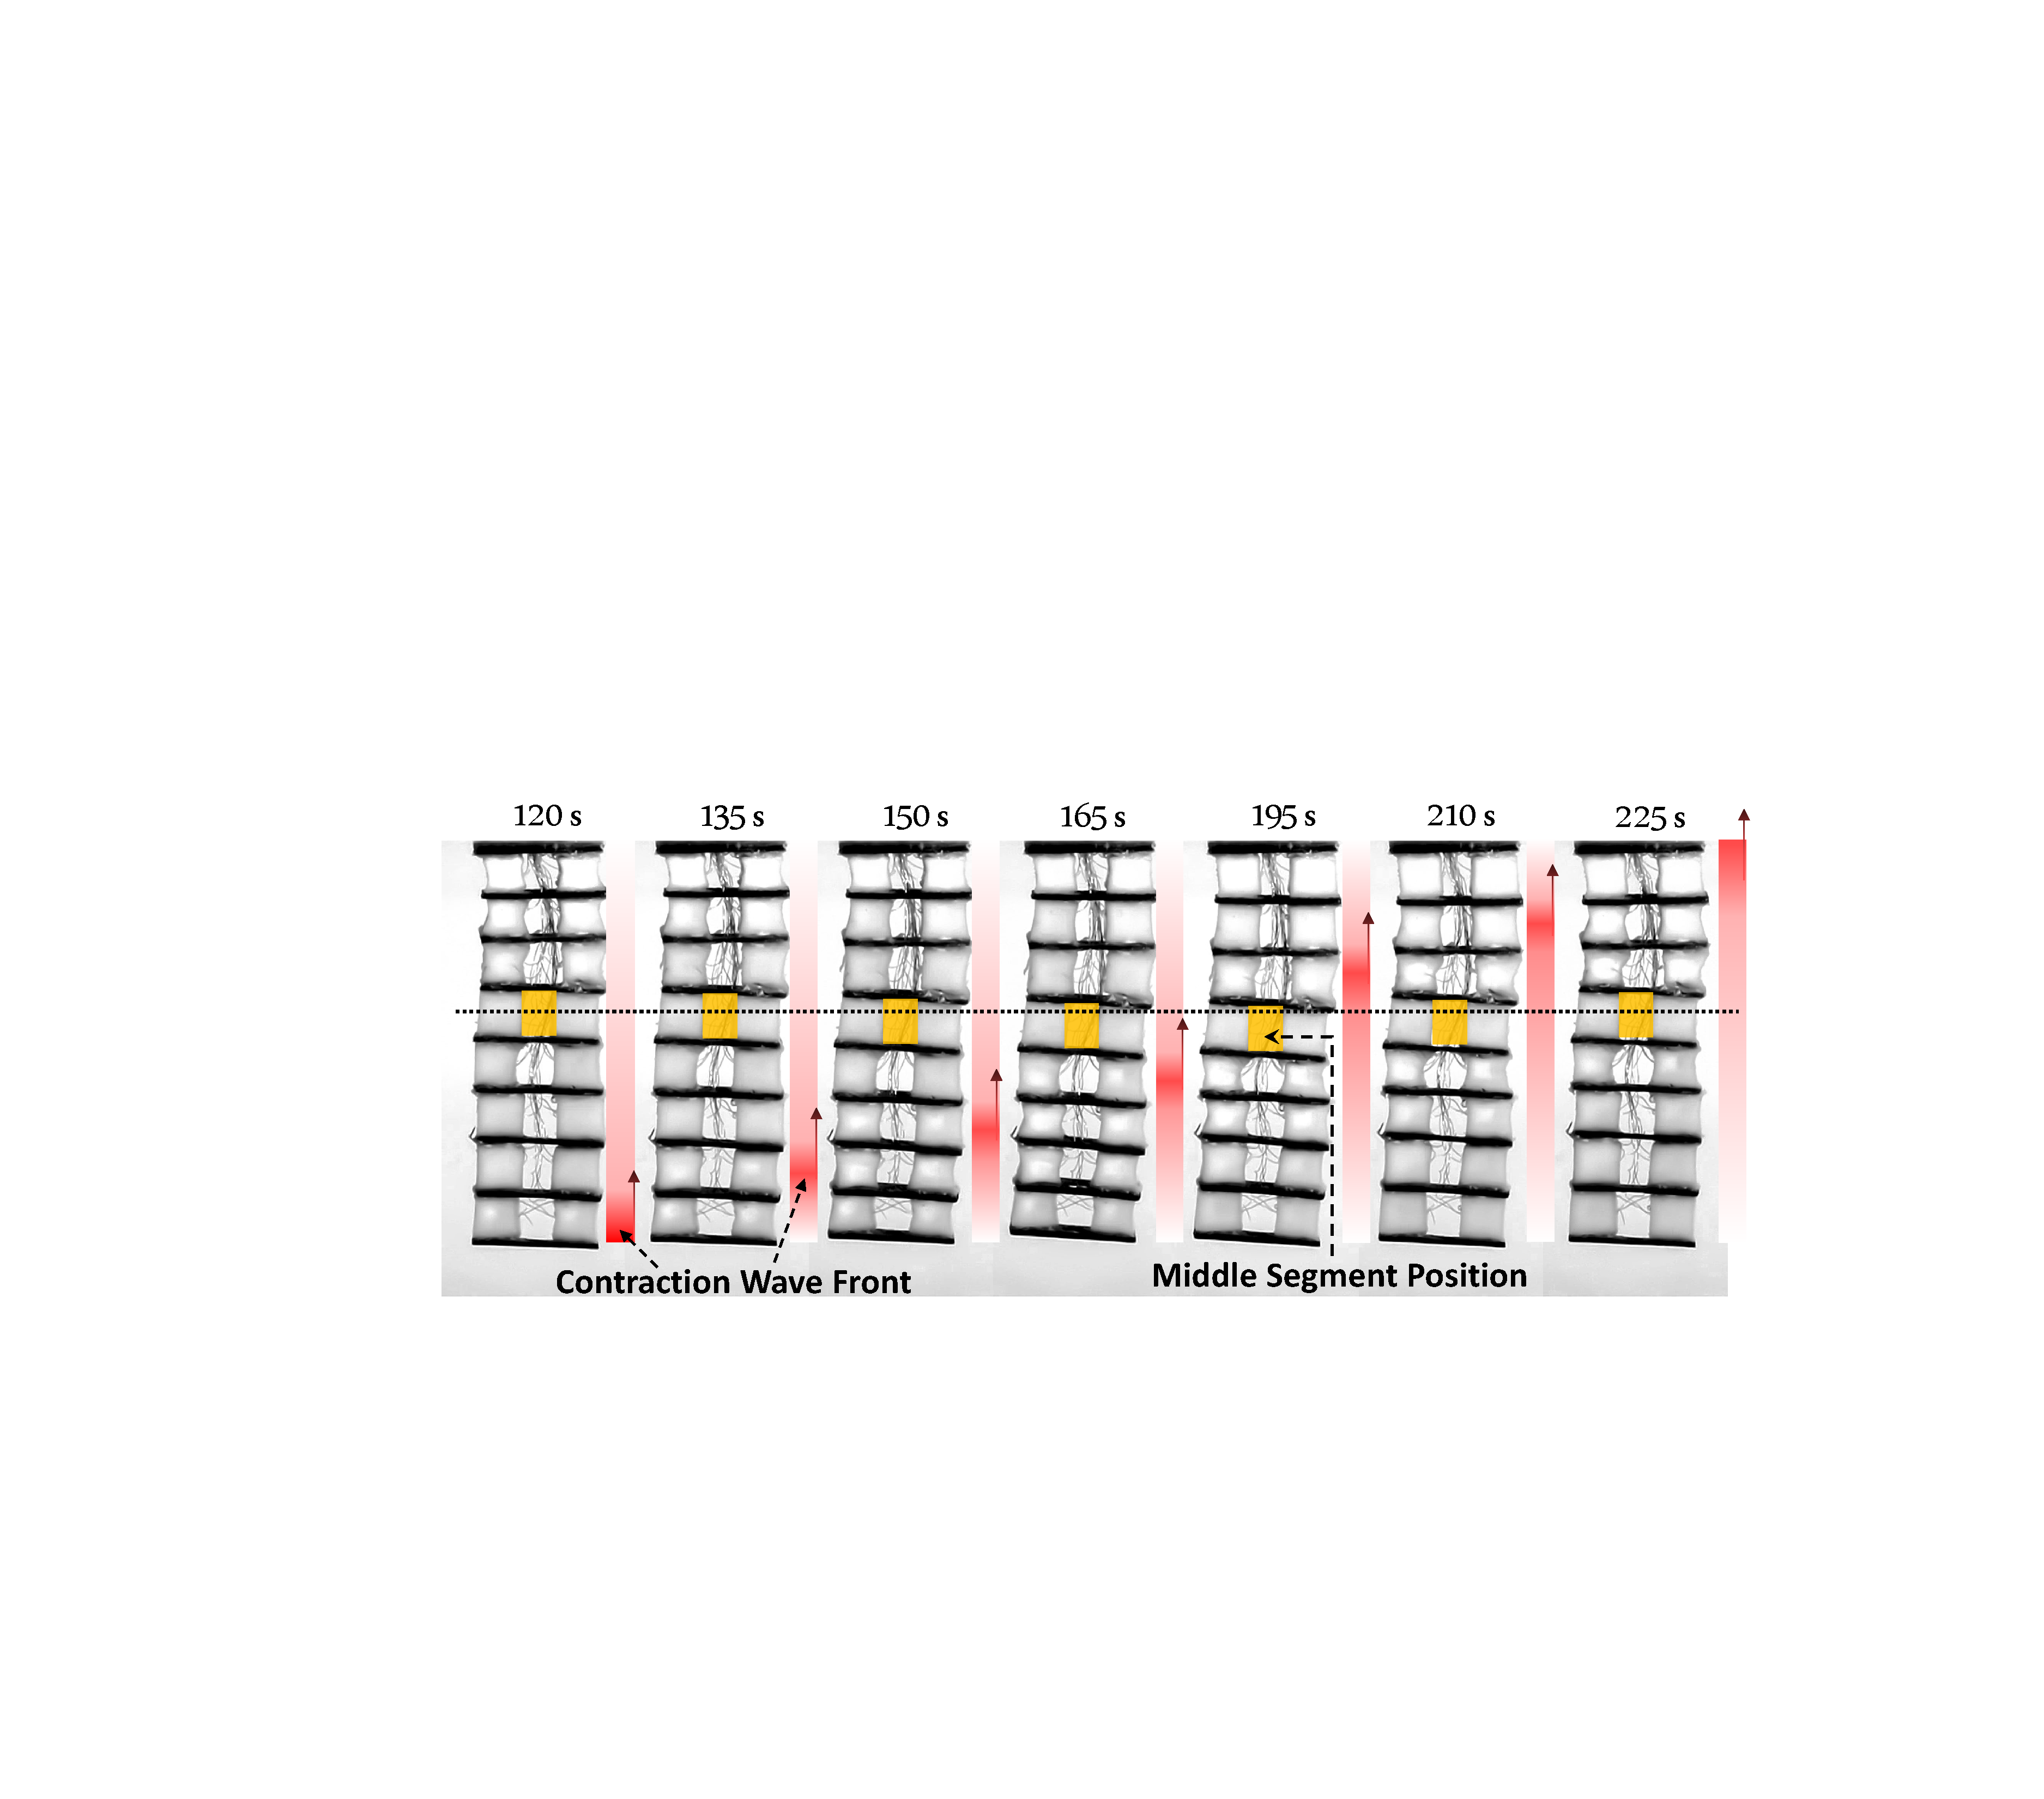
\includegraphics[width=\textwidth]{peristaltic.pdf}
\caption[The longitudinal traveling wave as it propagates through the structure]{The longitudinal traveling waves generated as a result of activation voltages shown in Figure~\ref{fig:sineWaves}. One SVA pair, indicated by the yellow square, is kept inactive in order to serve as a reference point. }
\label{fig:peristaltic}
\end{figure}


\begin{figure}[!ht]
\centering
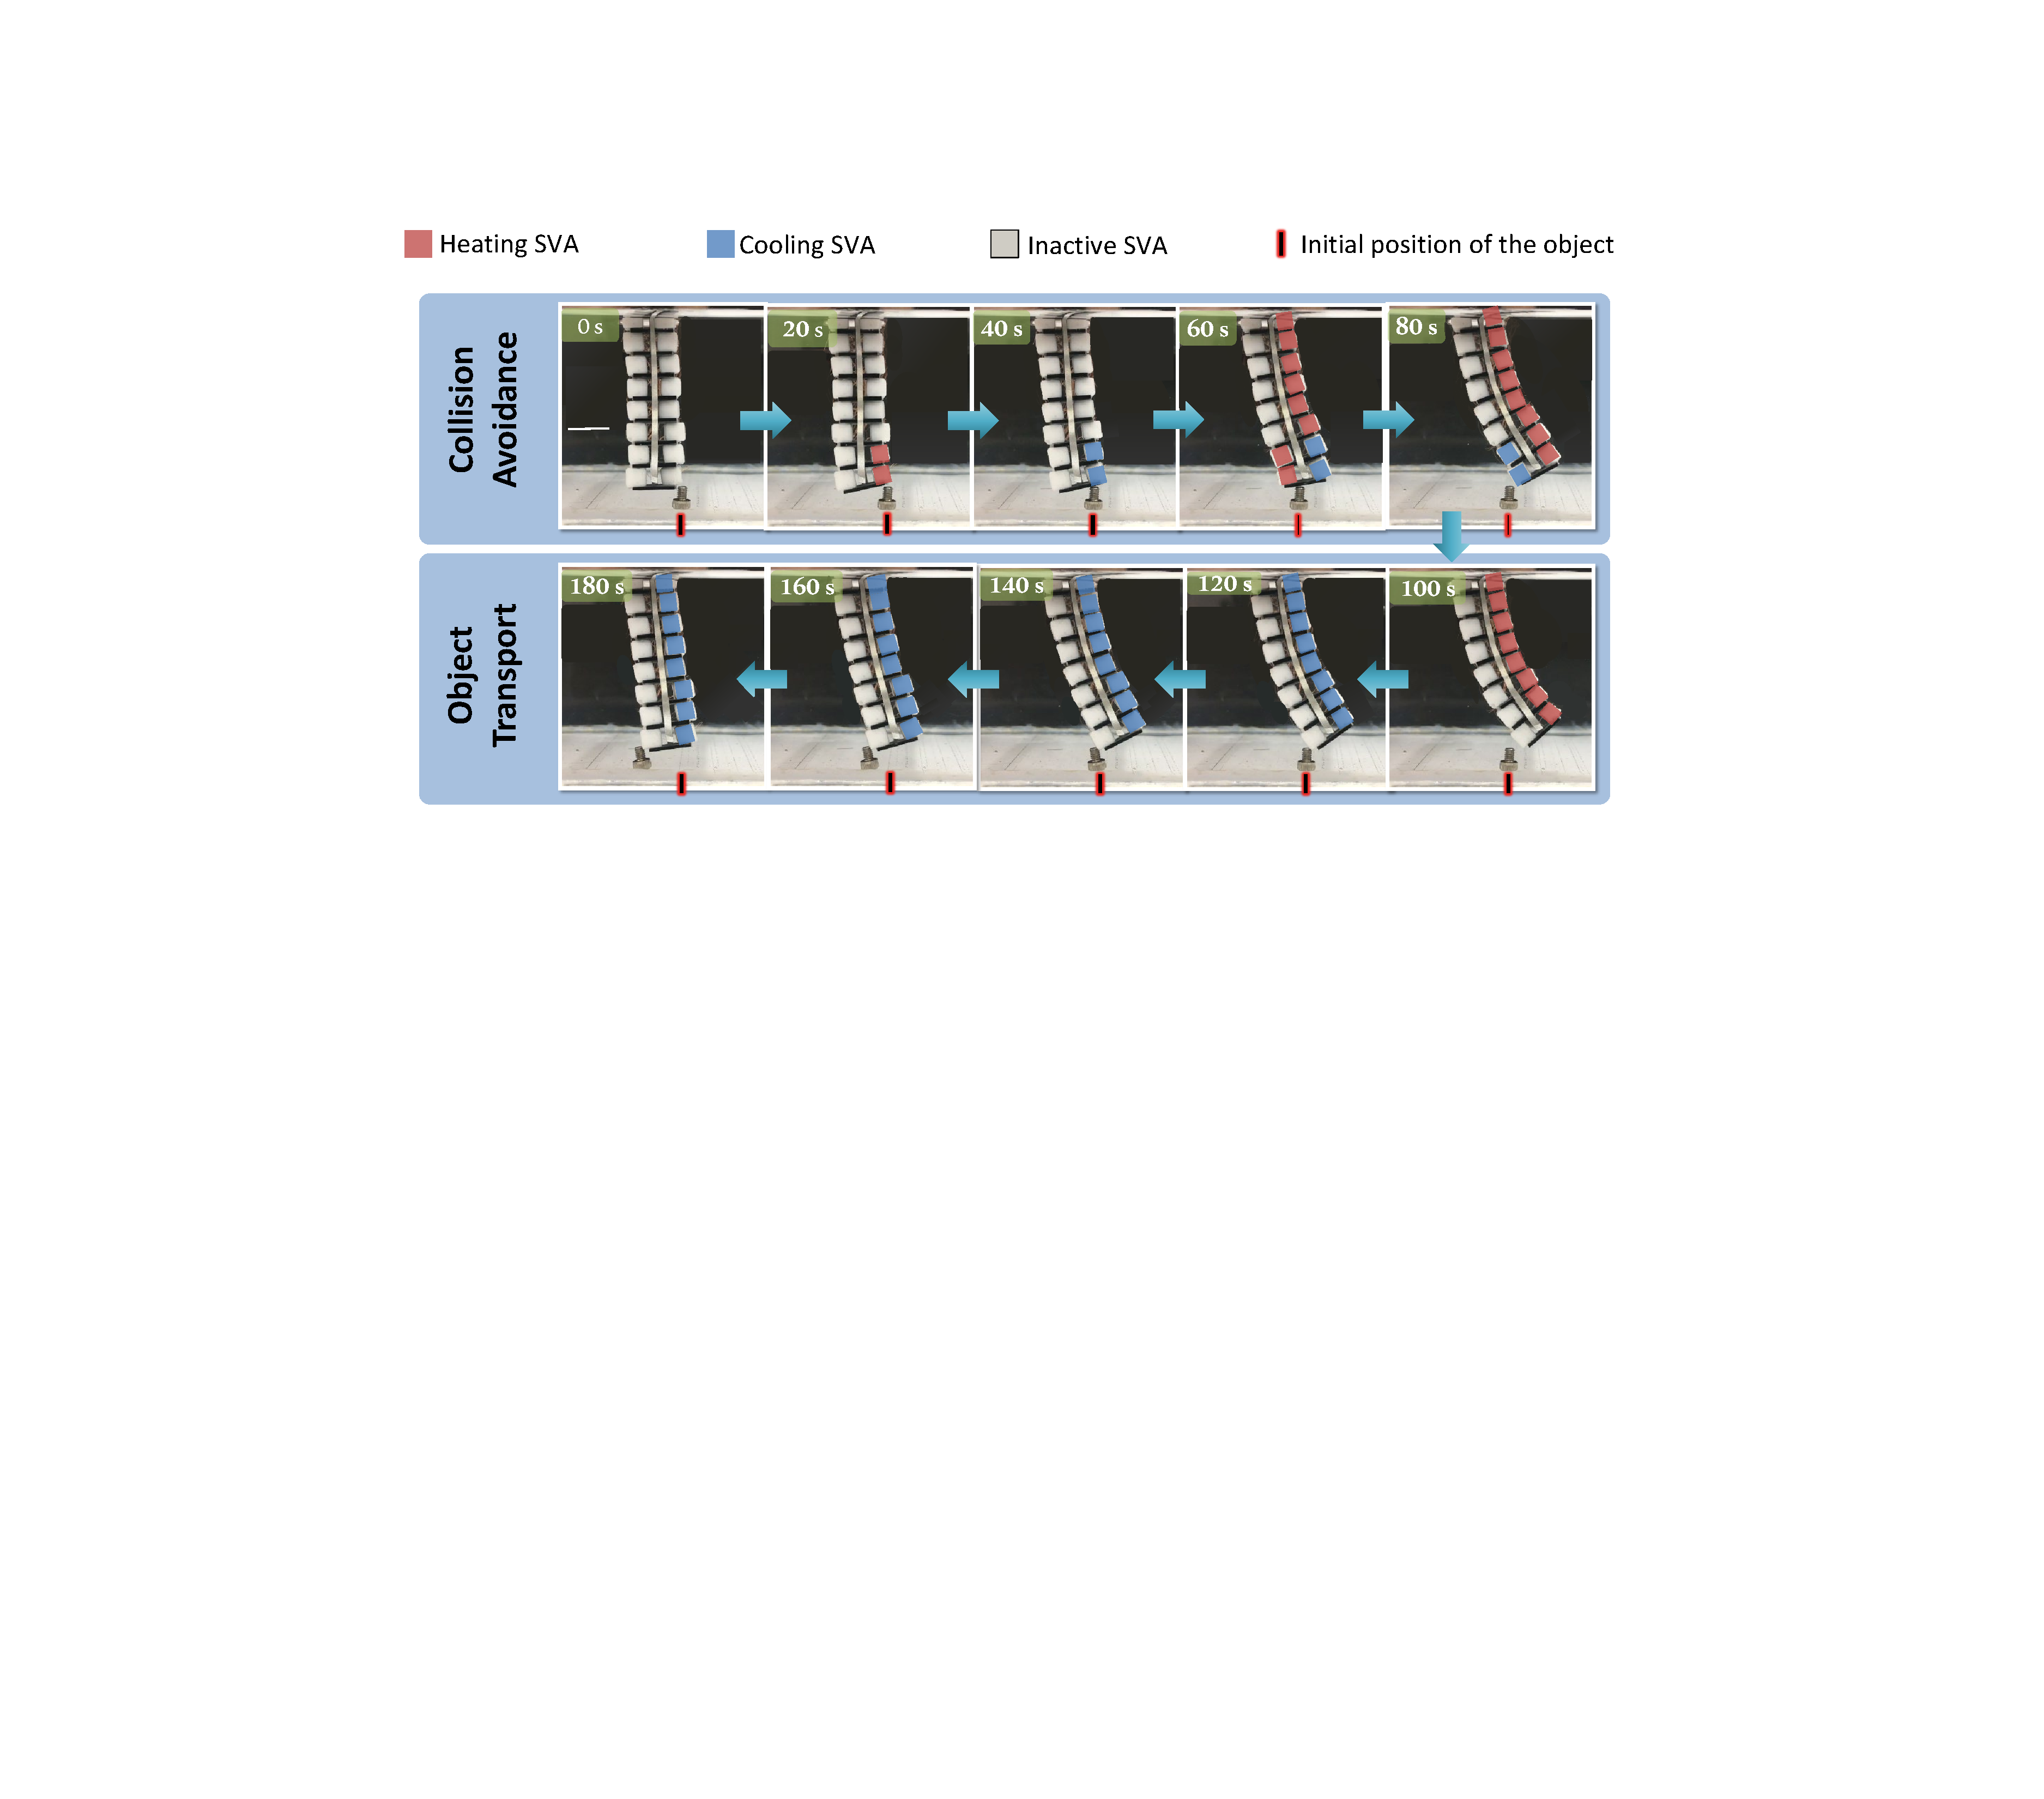
\includegraphics[width=\textwidth]{unstructured.pdf}
\caption[Dealing with unstructured environments]{Example usage of hyper-redundancy in manipulator with on-demand control of deformation. The structure can avoid collisions with objects or transport them, depending on the sequence of voltage commands from the microcontroller unit.}
\label{fig:unstructured}
\end{figure}

The ability to control the trajectory of the structure's end-effector, as shown in \figref{fig:armTrajOnOff}, is essential to successful functioning of the device in unstructured environments, in which working conditions may change during operation. As depicted in \firstfigref{fig:unstructured}, time-sequenced switching of selected SVA-II units within the structure makes it possible to accomplish various robotic tasks such as collision avoidance (top row) and object transport (bottom row). The trajectory of the end point $p$ and the angle $\theta$ of the end plate over time ($p$ and $\theta$ are defined in \firstfigref{fig:unstructuredTraj}) during each of these two tasks is displayed  in \subfigref{fig:4}{G}. The on-demand control of reorientation and translation of the end-effector made it possible to complete these two tasks, indicating that highly redundant time-varying deformations in heterogeneous structures are achievable using individually addressable SVA-II units.
\begin{figure}[!ht]
\centering
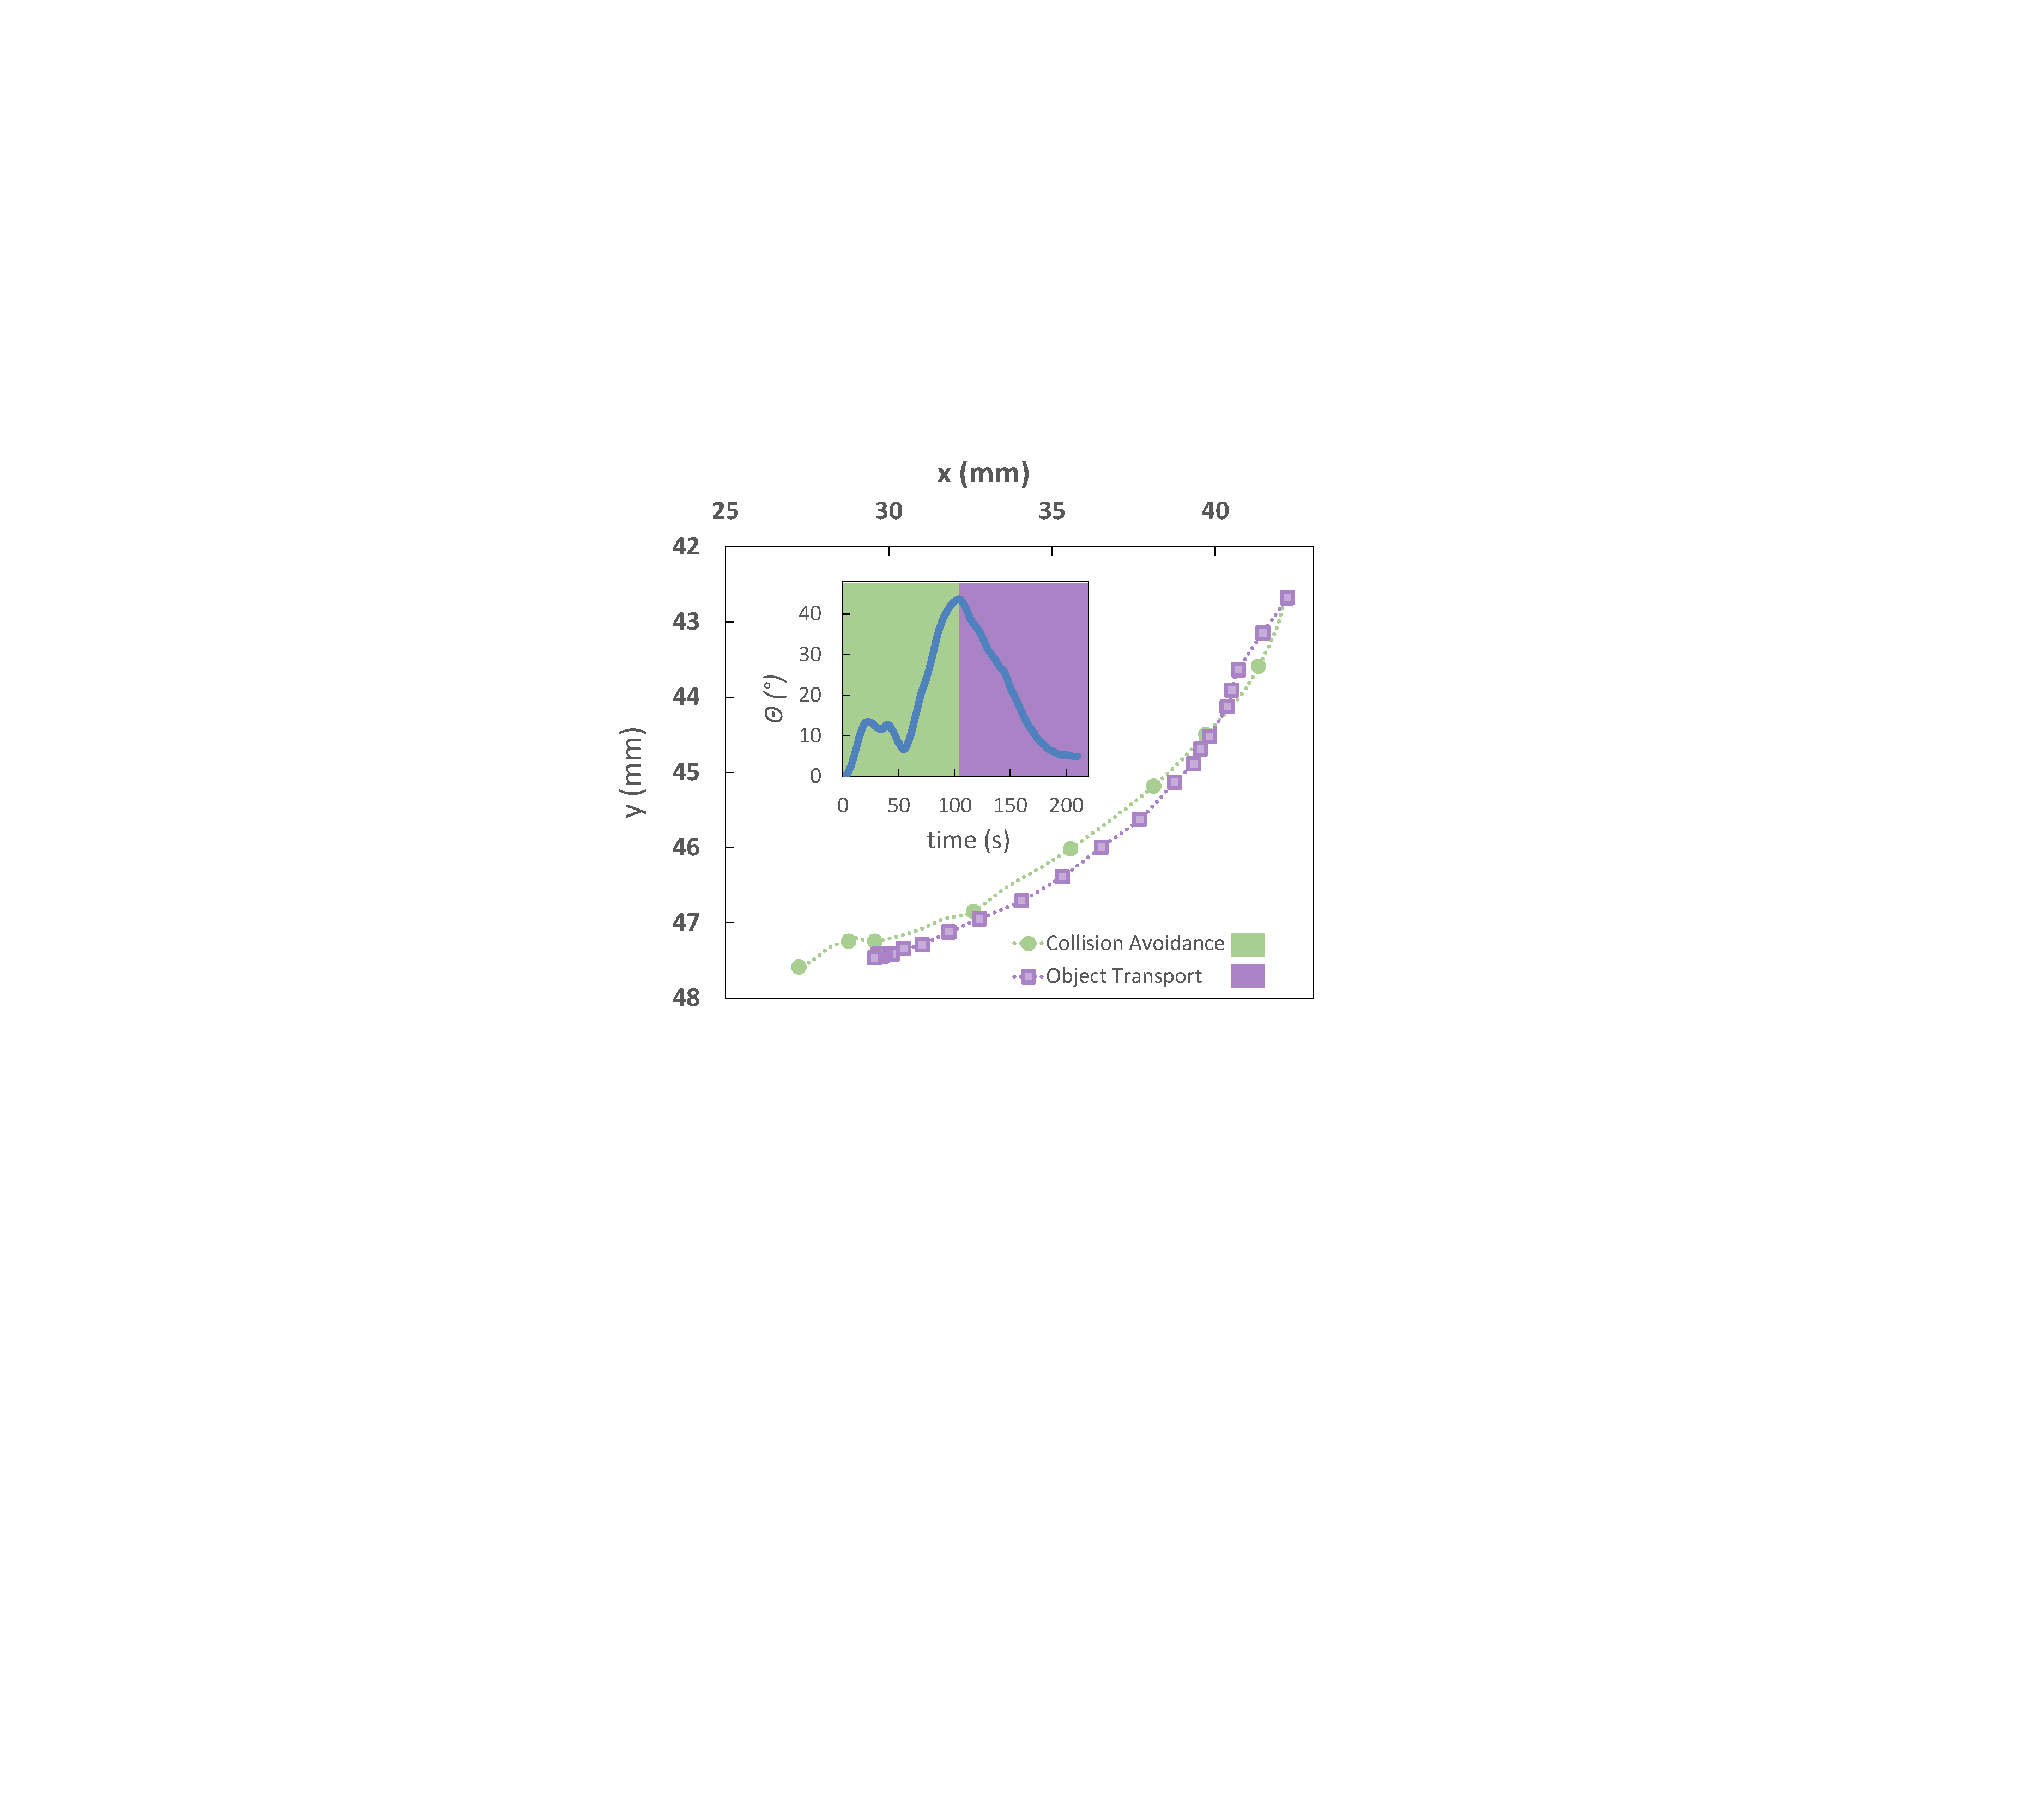
\includegraphics[width=0.8\textwidth]{unstructuredTraj.pdf}
\caption[On-demand creation of trajectories in unstructured environments]{Trajectory of the point $p$ on the tip of the structure as it first avoids and then transports the object. The inset shows the angle $\theta$ of the end plate as a function of time.}
\label{fig:unstructuredTraj}
\end{figure}


\section{Conclusions}
To summarize, we have developed the following tools to increase the variety and complexity of shape transformations in heterogeneous hydrogel structures: a voxel-based assembly design for patterning material domains, and a unique mixed-solvent photopolymerization hydrogel synthesis method for tuning swelling properties of the voxels. These tools offer a higher number of design parameters, namely, the configuration of the voxels, the material properties of each voxel, and the activation voltage of each voxel (in the case of SVA-II). This rich set of design parameters can be specified to build structures that meet the requirements of a variety of tasks. The resulting heterogeneous structures can generate complex time-varying trajectories and traveling waves, enabling them to interact with unstructured environments in ways that could not be realized in bulk hydrogels or that would require sophisticated integration and manufacturing.\\

The simplicity of these tools advances the utility of hydrogel structures in robotics applications in a meaningful way because they can be used in robotics research laboratories that lack sophisticated material processing facilities.

While this dissertation focuses specifically on PNIPAAm hydrogel voxels, soft and rigid voxels made of other types of responsive or non-responsive materials can also be incorporated into heterogeneous assemblies. Closed-loop control of the deformation of the structures presented in this dissertation could be achieved by integrating strain- and force-sensitive voxels, made of similar functional hydrogels, that serve as sensors. In addition, multi-objective optimization across material properties and voxel configurations can be used to design structures with higher force production capacity and %higher 
energy efficiency. Currently, integrating multiple active degrees of freedom (DOFs) in miniaturized soft robots is challenging due to space limitations. Each SVA can be considered as an active DOF and we have demonstrated that the integration of a high number of SVAs in a small footprint, such as the 16-voxel structure presented in this chapter, is possible. To address the challenges of fabricating large-scale 
assemblies consisting of hundreds of voxels, % is still challenging and
automated methods must be developed for scalable manufacturing and assembly of voxels.
\graphicspath{{Images/untetheredWalker/}}

\chapter{Miniature Untethered Underwater Walking Robot}
\label{chap:untetheredWalker}
Current soft actuators rely on additional hardware such as pumps, high voltage supplies, light generation sources and magnetic field generators for their operation. 
% Assembling these actuators results in bulky robotic systems, although the body of the soft robot itself may remain miniaturized. 
These components resist miniaturization and embedding them into small-scale soft robots would be challenging. This limits their mobile applications where the entire system needs to be untethered especially in hyper-redundant robots where a high number of actuators are needed. Here, we introduce miniature and untethered robots made of soft voxel actuators (SVAs) -- an active voxel using stimuli-responsive hydrogels actuated by electrical currents through Joule heating. SVAs weighing only 100\,mg require small footprint microcontrollers for their operation which can be embedded in the robotic system. We have demonstrated the advantages of hydrogel-based SVAs through a hyper-redundant manipulator with 16 actuators and an untethered miniature robot for underwater mobile applications.
\section{Background}
Inspired by biology, soft robot developers try to utilize the advantages inherent in soft, compliant matter to achieve safer interactions around humans or more robust locomotion and manipulation in unstructured environments~\cite{martinez2013robotic,laschi2012soft,tolley2014resilient,bilodeau2015monolithic}.  
Soft pneumatic actuators (SPAs)~\cite{Gorissen2017, branyan2017soft} are the most widely used category in soft robotics. SPAs use passive materials such as silicone and rely on rigid components such as motors and pumps that are difficult to downscale and therefore, manufacturing small-scale soft actuators which have applications as envisioned by \cite{hines2017soft} has remained a bottleneck in the development of miniaturized soft robots \cite{majidi2019soft}. 

Stimuli-responsive, soft materials have shown promise in solving some of these challenges \cite{steele2018stimuli, stuart2010emerging,white2013advances}. The changes in the stress/strain distribution in these materials in reaction to variations in pH, temperature, electric field, magnetic field, and light results in motions such as bending, twisting, or elongation. However, the equipment needed to create variable stimuli such as structured light \cite{palagi2016structured} or magnetic field \cite{Kim2018} are still bulky. Temperature responsive hydrogels, by contrast, can be stimulated electrically using Joule heating \cite{yu2013electronically}. The electrical stimulation can be confined to small regions making it possible to create more precise motions \cite{richter2009optoelectrothermic}. We have previously reported solving some of the challenges associated with temperature responsive poly(N-isopropylacrylamide) (PNIPAAm) based hydrogels such as their slow response and tuning their mechanical properties. We have also introduced blocks called soft voxel actuators (SVAs), which are electrically activated by Joule heaters \cite{Khodambashi2021}. In this communication, we demonstrate how SVAs support the development of soft robots which are miniature and untethered --two key characteristics that are challenging to realize with pneumatic soft actuators. We introduce a miniature completely untethered robot for underwater applications which weighs only 20\,g including battery and electronics as shown in Fig.~\ref{fig:concept}. We also demonstrate the use of SVAs to build a miniature continuum manipulator with hyper-redundant DOFs as shown in Fig.~\ref{fig:treajectory}A. This manipulator is 10$\times$ 40 $\times$ 4.5\,mm$^3$ and has 16 actuators. 

\begin{figure}[!t]
\centering
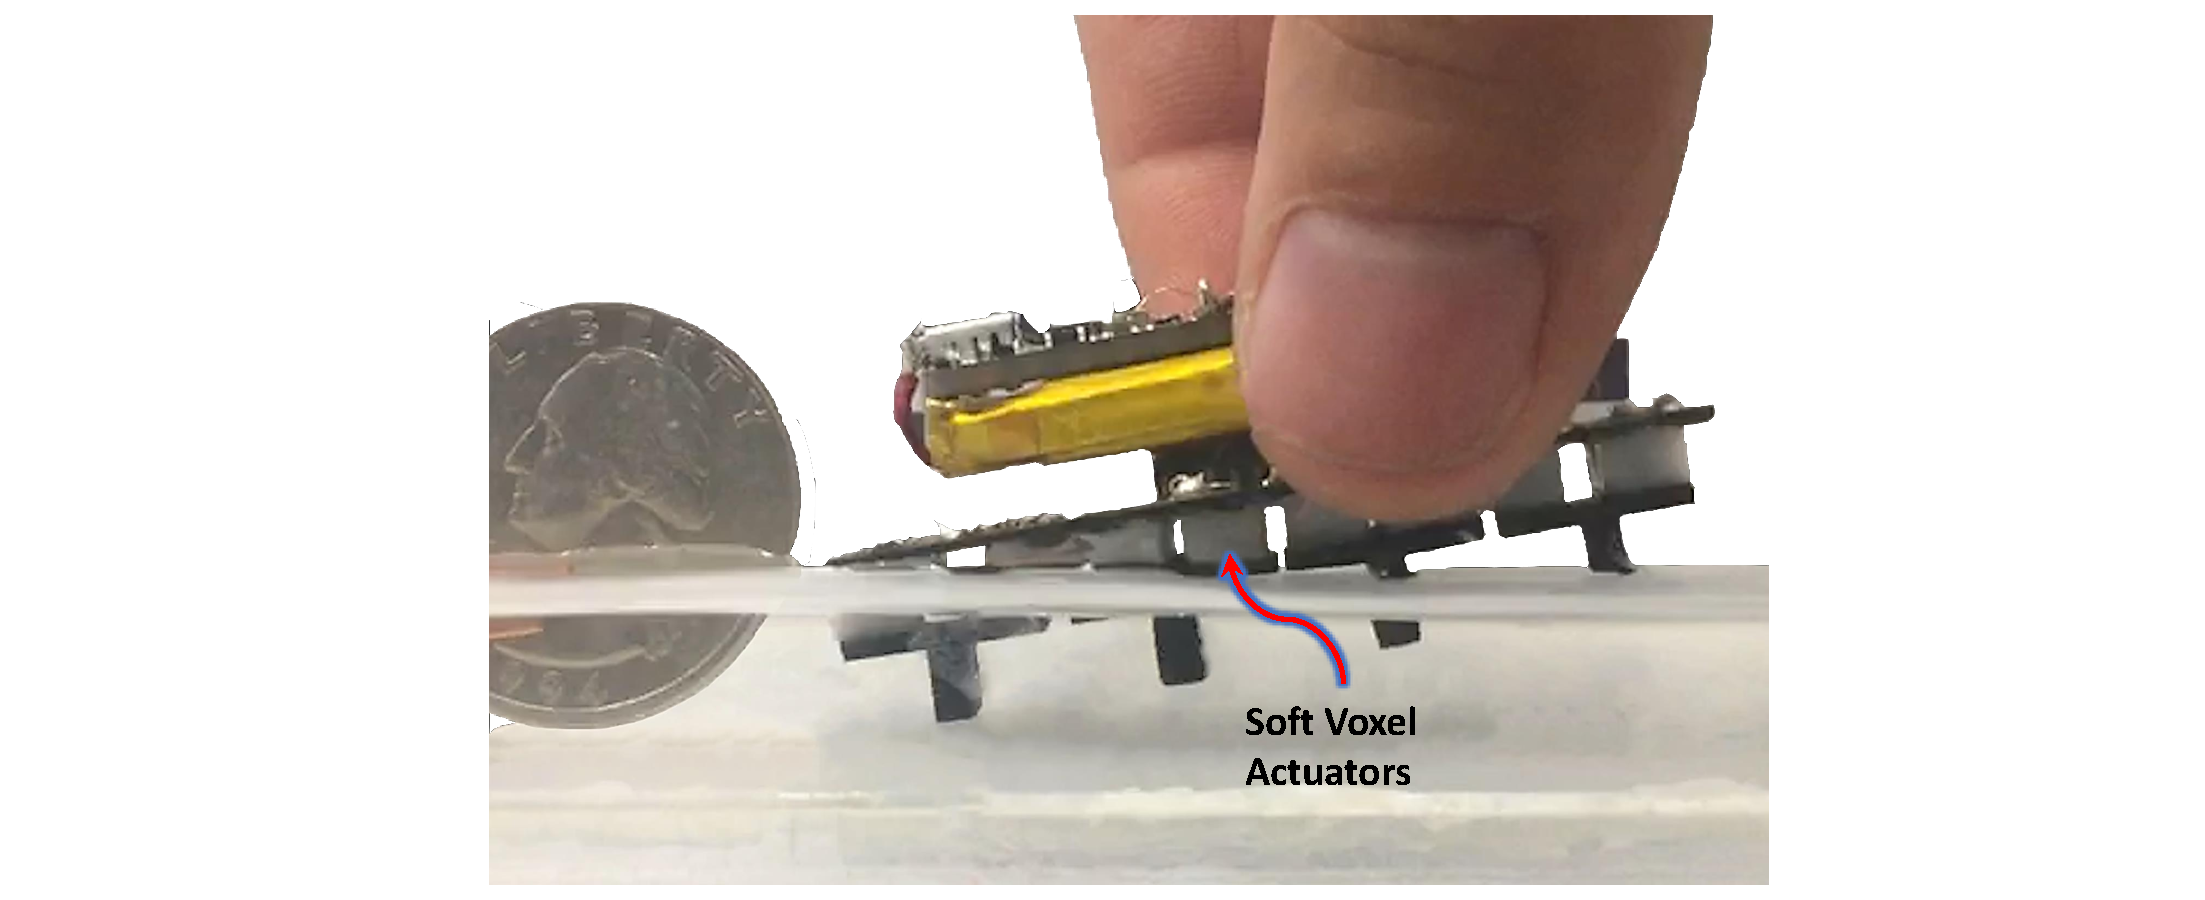
\includegraphics[width=0.7\textwidth]{Fig1.pdf}
    \caption{Soft Voxel Actuators (SVAs) are individually addressable hydrogel-based actuators that can aid in miniaturizing and cutting the tether from soft robots. 
    % A) A hyper-redundant miniature manipulator using 16 SVAs. B) 
    An exemplary untethered miniature underwater walking robot using 8 SVAs is shown which weighs only 20\,g including battery and electronics.}
    \label{fig:concept}
\end{figure}
\begin{figure*}[!t]
      \centering
      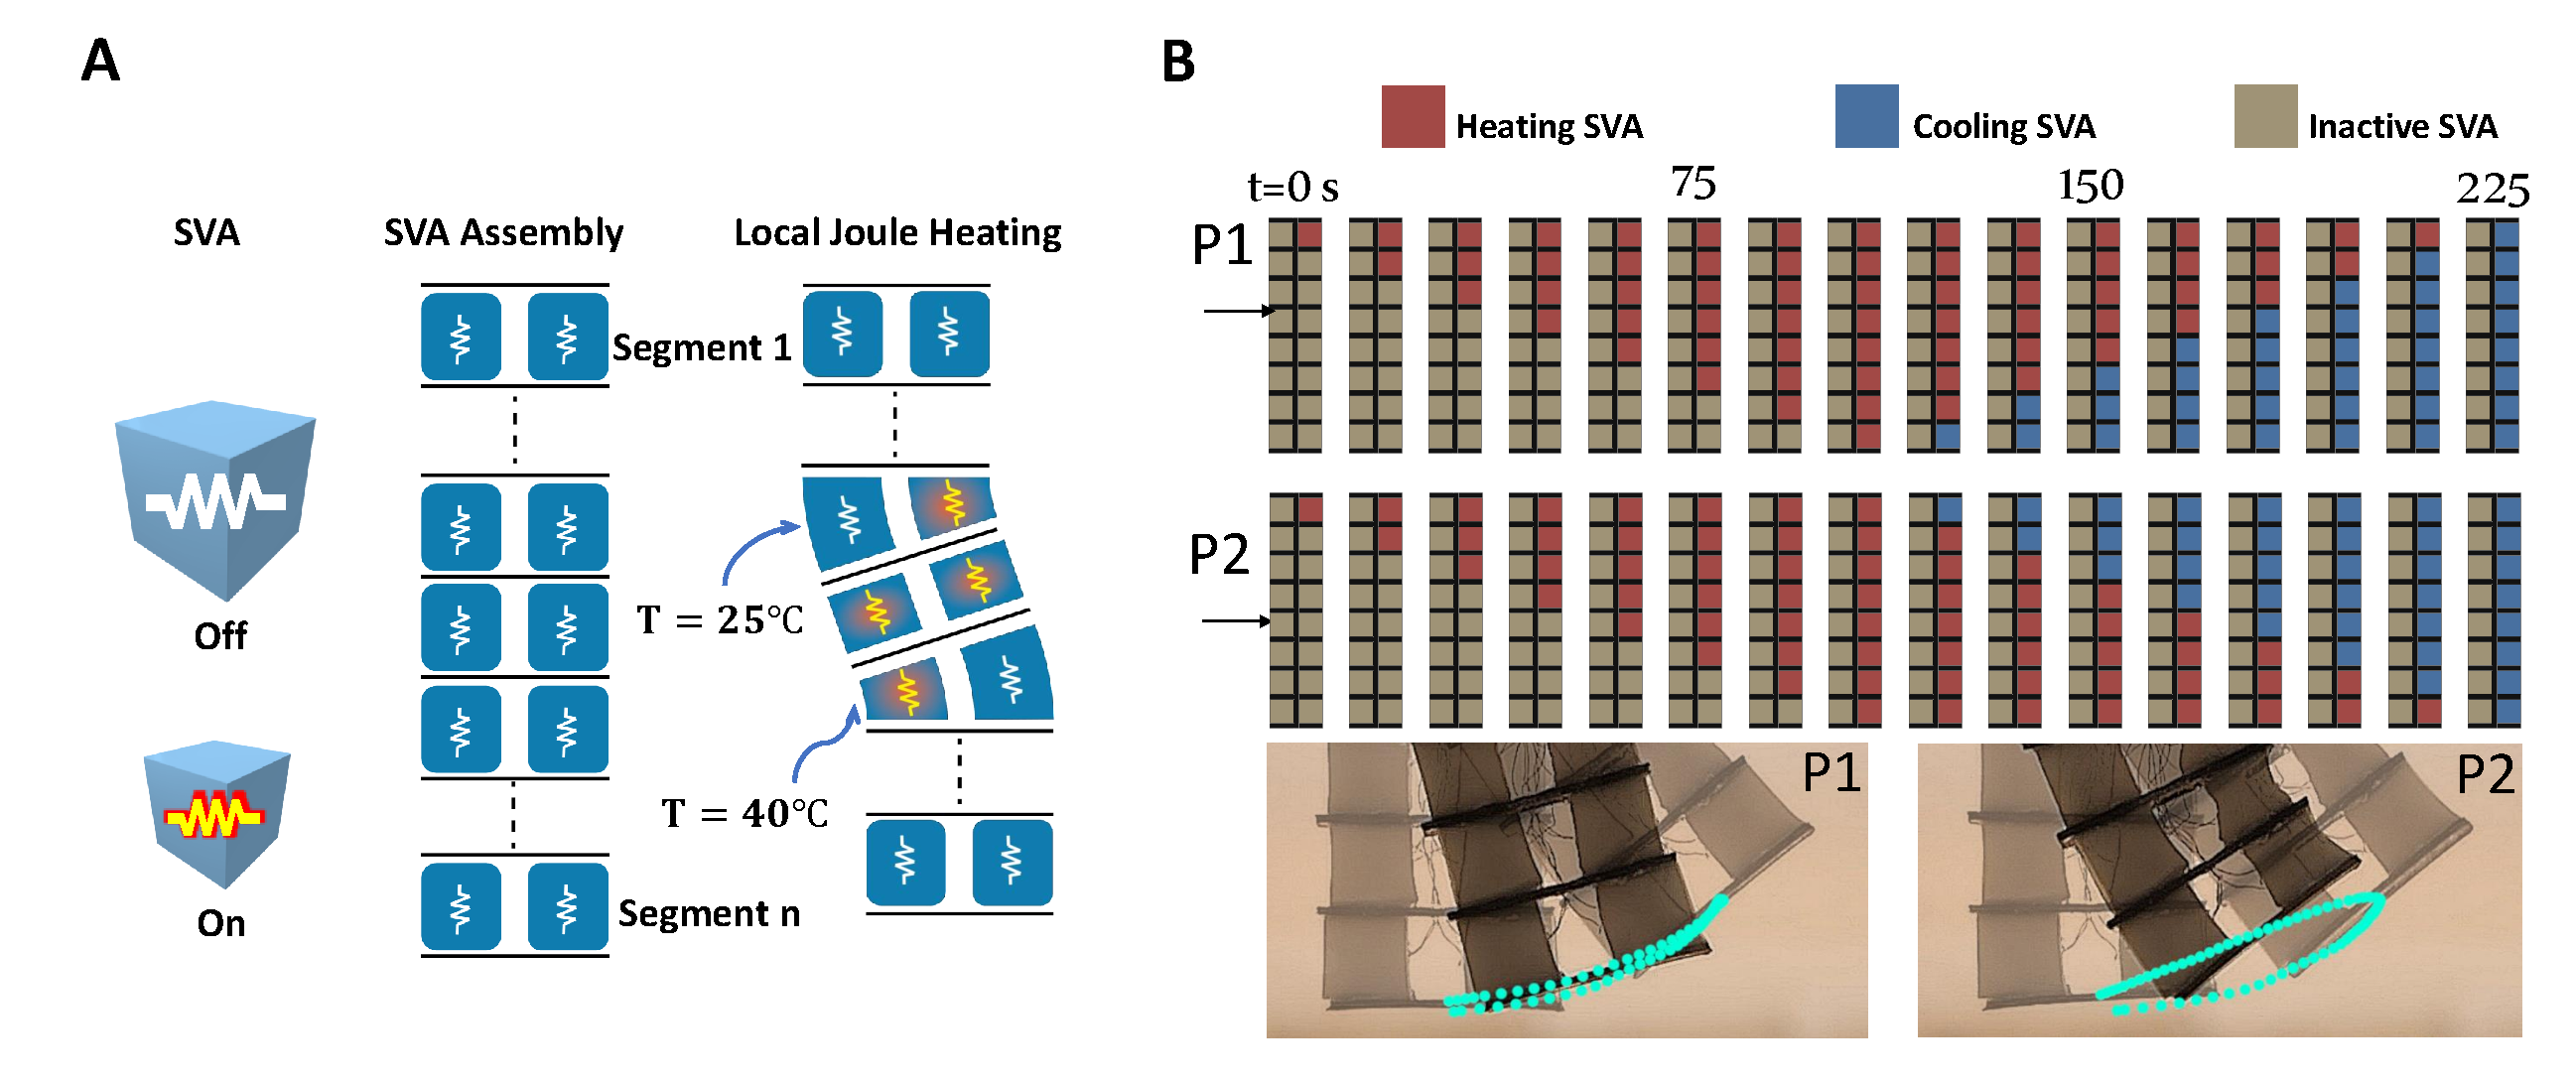
\includegraphics[width=\textwidth]{Fig2.pdf}
      \caption{A) On and off states of a SVA is shown on the left column. Schematic of an assembly of SVAs is shown on the middle column. Activation of SVAs results in local increase in the temperature which leads to deformations that control the overall motion of the manipulator (right column). B) Sequentially activating SVAs 1 through 8 according to the patterns labeled P1 and P2 results in different trajectories followed by the tip of the manipulator (shown in cyan at the bottom). For details, see Movie S1.}
      \label{fig:treajectory}
   \end{figure*}
	
\section{Soft Voxel Actuators (SVAs)}
A voxel actuator can be made in different shapes and dimensions based on the design requirements. Manufacturing a SVA is performed via a molding process in which a hydrogel precurosor solution is poured into a mold, a Joule heater is inserted in the mold and then the solution is polymerized with a UV LED. Surface  mount  resistors  (10\,ohm  SMD  resistor  0805) were chosen as the heating elements. For the construction of the hyper-redundant manipulator, the voxels are made as cubes of 4.5$\times$4.5$\times$4.5\,mm$^3$ as shown in Fig.~\ref{fig:treajectory}A. In case of the untethered walking robot, voxels of 8$\times$4.5$\times$3\,mm$^3$ are used. Details of hydrogel synthesis, material characterization and SVA manufacturing are discussed in \cite{Khodambashi2021}.

\section{Results}
Hydrogels expand and contract based on the diffusion of water into and out of their structure when the temperature is passed their critical transition temperature -- which is around 32\textsuperscript{o} C in case of PNIPAAm hydrogels. Therefore, all the experiments are performed in a water bath. Fig.~\ref{fig:treajectory}A shows a schematic of a SVA. When the embedded Joule heater is turned on, the temperature increases and the volume of the hydrogel is decreased. When the heater is turned off the SVA cools down and its volume increases. We have shown that a SVA can produce a force of 0.12\,N which is equivalent to a weight of nearly 12\,g. This is 120 times its own weight \cite{Khodambashi2021}. To demonstrate how SVAs support the development of miniature and untethered soft robots, we describe two different robotic platforms in the following sections. 
\subsection{Case Study I: Miniature Hyper-redundant Soft Robotic Arm}
The structure shown in Fig.~\ref{fig:concept}A was assembled using 16 SVA units. The SVAs are connected together using a 0.1 mm thick 3D printed PLA sheets. Dynamic on-demand shape changes are achieved through time-varying activation of SVAs.
As demonstrated in Fig.~\ref{fig:treajectory}B, the choice of SVA actuation pattern can influence the end-effector trajectory of the manipulator. In this experiment, SVAs 1 thorough 8 are activated according to patterns denoted by P1 and P2. Movie S1 shows the resulting trajectories for P1 and P2.
% in \subfigref{fig:4}{D}. 
Each SVA is activated with maximum voltage (3.7\,V) for 15\,s before the next SVA is activated.
The demonstrated miniaturized continuum manipulator with 16 degrees of freedom in a $40\times11\times5$\,mm$^3$ footprint represents the highest reported electrically-addressable number of DOFs in a soft manipulator of these dimensions. 
\subsection{Case Study II: Untethered Miniature Underwater Walking Robot} 
\begin{figure*}[!t]
      \centering
      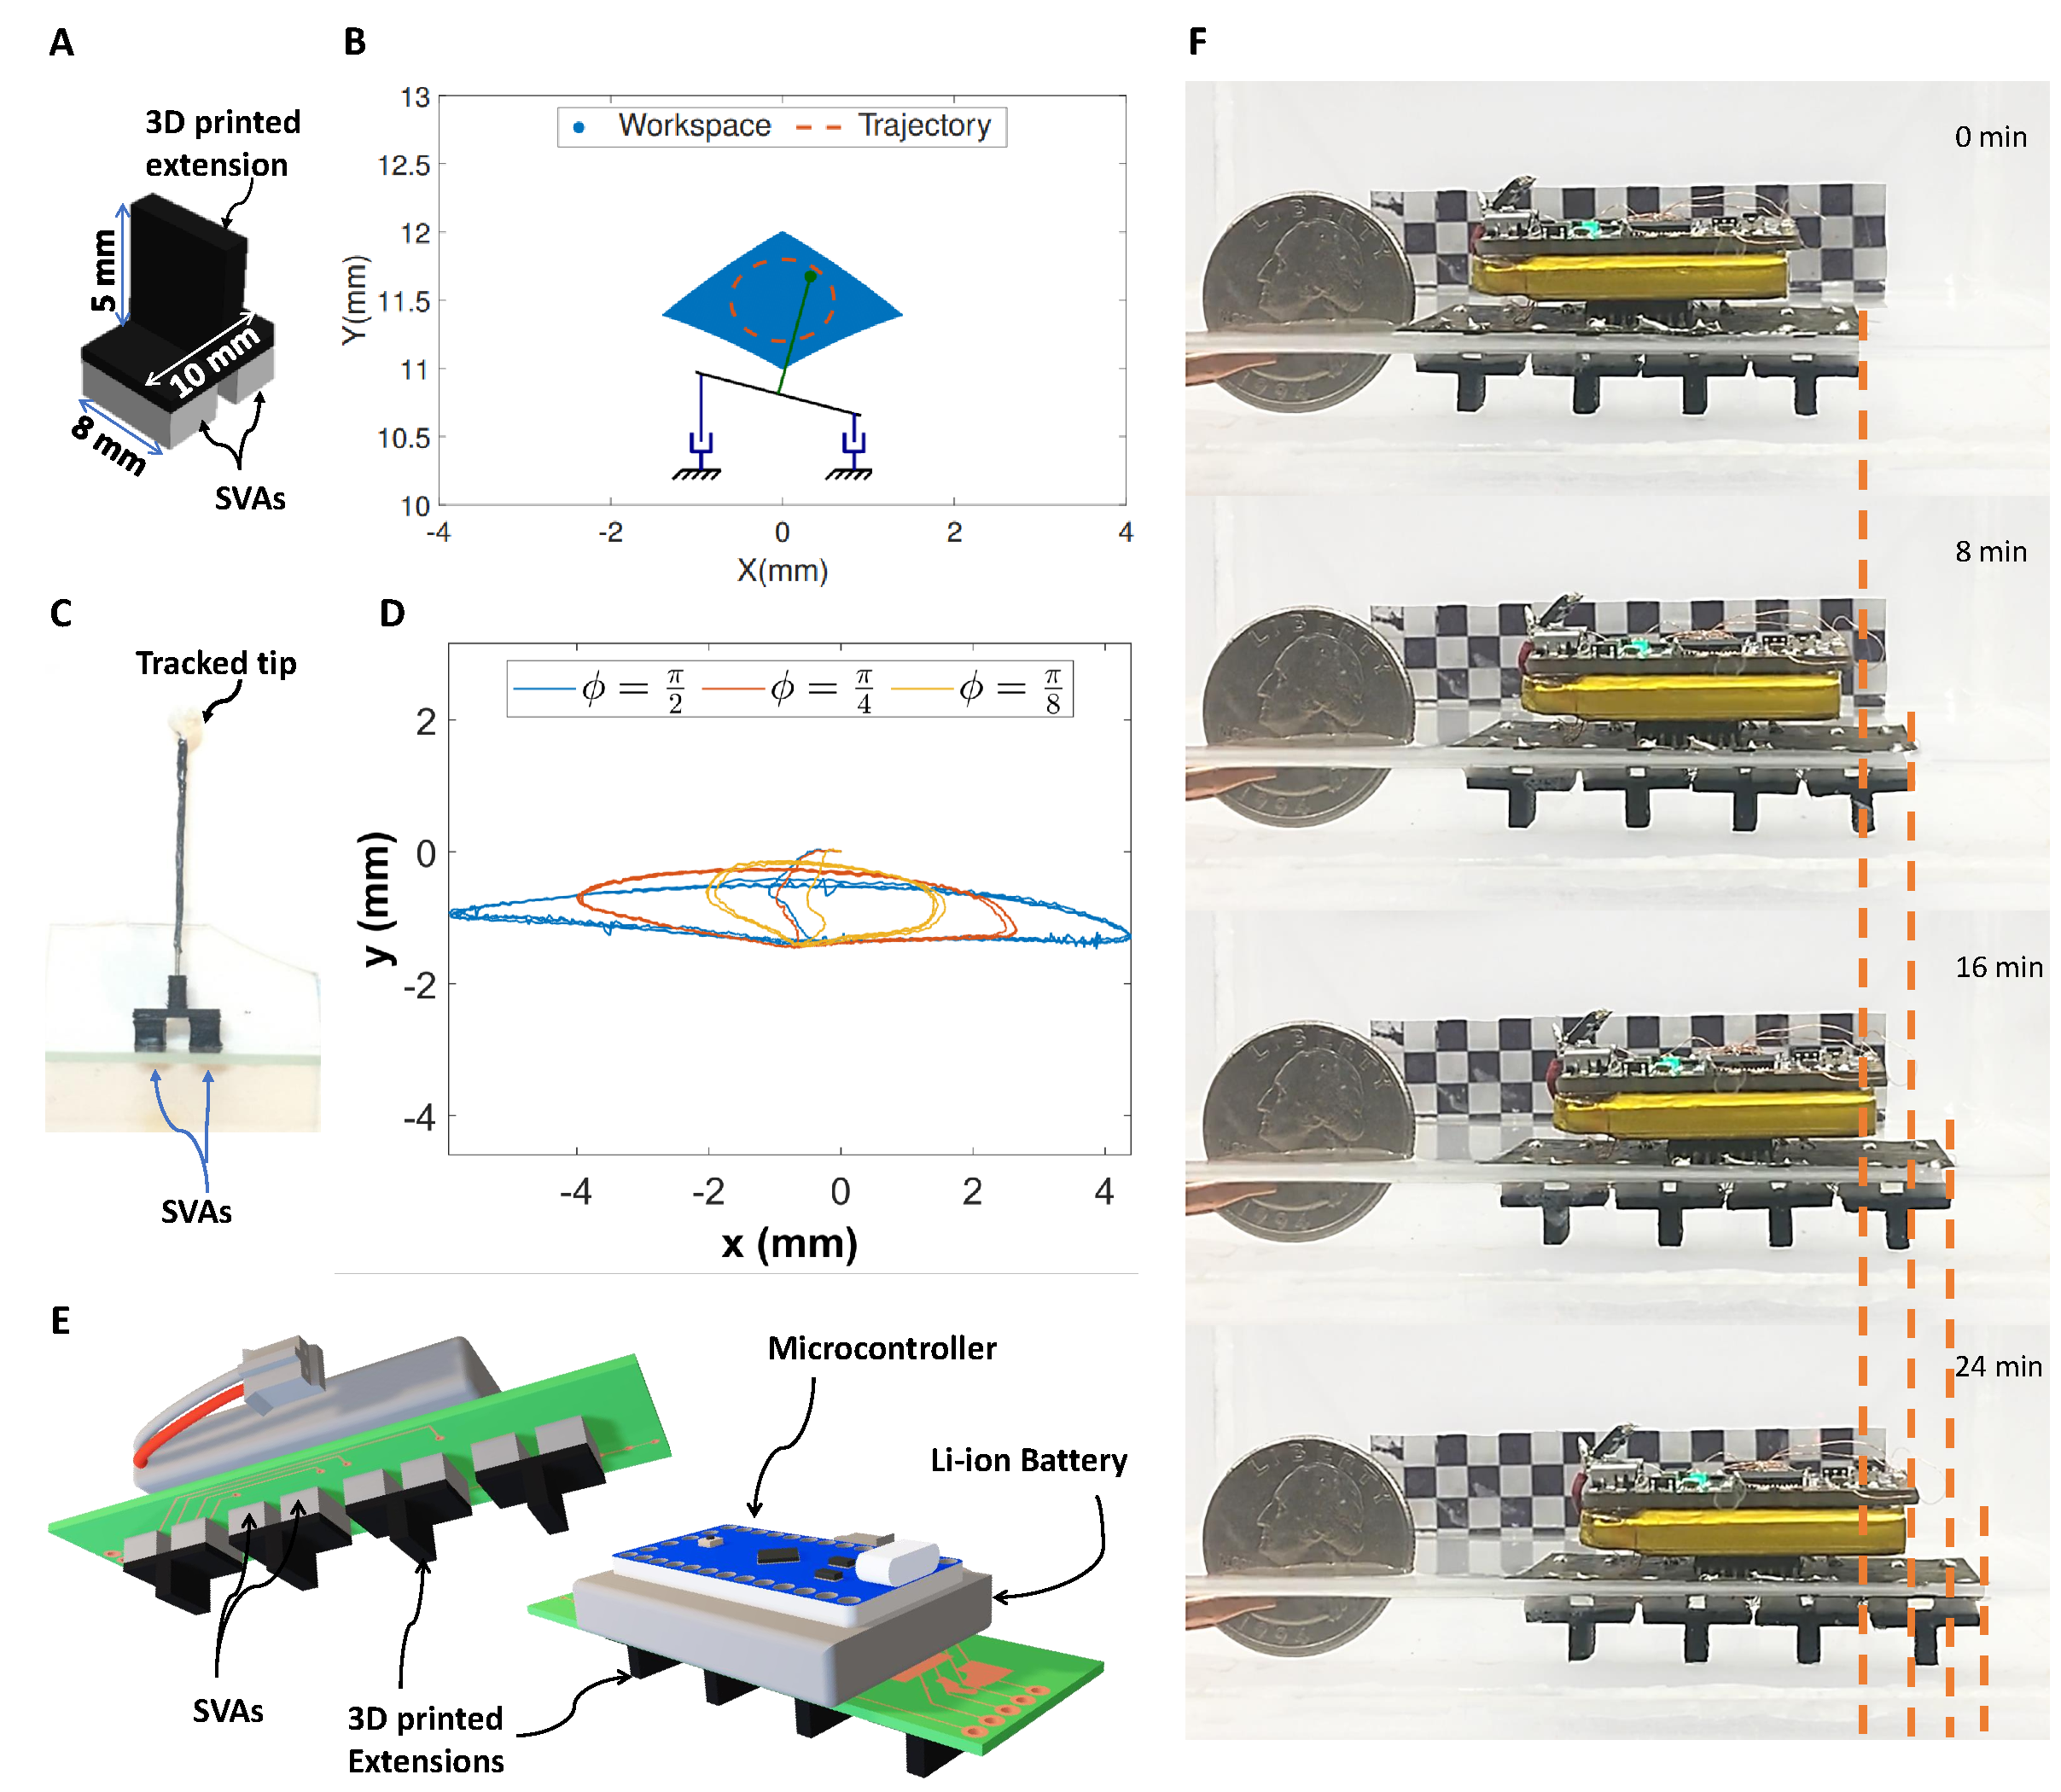
\includegraphics[width=1\textwidth]{Fig3.pdf}
      \caption{A) A two degrees of freedom manipulator using two SVAs and a 3D printed extension. B) The workspace of the tip of this manipulator. C) A needle is attached to the tip of the 3D printed extension to amplify the movement of the tip. D) Different trajectories of the tip of the needle as a function of phase shift in the sinusoidal excitation voltages. E) A microcontroller board and a lithium ion battery is added to the system to make an untethered robot. F) Time-lapse of the movement of the miniature underwater walking robot (see Movie S1 for details).}
      \label{fig:untethered_podia}
\end{figure*}
The robot shown in Fig.~\ref{fig:concept}B has four legs. Each leg is a two DOF manipulator composed of 
% To demonstrate the above mentioned features, we have developed a manipulator using 
two SVAs and a 3D printed extension as shown in Fig.~\ref{fig:untethered_podia}A. The workspace of the tip of this manipulator is plotted in Fig.~\ref{fig:untethered_podia}B. To amplify the movement of the tip and measure it more precisely, a needle is attached to the tip of the 3D printed extension. A spherical marker is attached to the end of the needle and functions as a marker for tracking using a camera (Fig.~\ref{fig:untethered_podia}C). The needle is only attached for recording the trajectories and was not present in the final robot prototype. We have created circular and oval trajectories using sine wave voltages as input to the SVAs. Each SVA is actuated using a sine wave with a phase shift with respect to other SVA. As the phase shift between the two SVAs in a manipulator is varied, the shape of the trajectory changes. Fig.~\ref{fig:untethered_podia}D shows different trajectories of the tip of the needle as a function of phase shift in the sinusoidal excitation voltages. To create an untethered walking robot, four manipulators discussed above are assembled in an array. The array is attached to a microcontroller board (Adafruit Itsy Bitsy M0) and a lithium ion battery is added to the system as shown in as shown in Fig.~\ref{fig:untethered_podia}E. The movement of the miniature underwater walking robot is shown as a time-lapse in Fig.~\ref{fig:untethered_podia}F and also can be seen in details in Movie S1.
\section{CONCLUSIONS}
We have shown that the voxel-based design and manufacturing strategy, combined with an electrically addressable smart material, can lead to the creation of miniaturized soft robots with a high number of DOFs. These robots can be used for tasks in which redundancy is needed for example to handle continuously changing tasks in unstructured environments. This has been demonstrated through a miniaturized hyper-redundant soft robot with 16 SVA units.
SVAs can be easily integrated into robotic systems. They help greatly reduce the size of the robots. In addition, sice the SVAs are electrically controlled, they can be connected directly to small footprint microcontrollers and other electronics. The electronics and power supply can be embedded in the robot  and cut the tether from the entire system. We have demonstrated this through a miniature underwater walking robot that do not rely on external signals or power which can be beneficial in applications such as under water data collection and ocean monitoring. The SVAs introduced in this paper are the first demonstration of active, soft voxels that are made of stimuli-responsive materials. Using SVAs as building blocks offers higher number of design parameters, namely, the configuration of the SVAs, the material properties of each SVA, and the activation voltage of each SVA. Multi-objective optimization can be used in future to optimize this rich set of design parameters to build structures that have higher force production capacity and %higher 
energy efficiency.
% miniature and micro-scale soft actuators have matured more slowly than their  macro-scale counterparts. 


\graphicspath{{Images/conclusion/}}

\chapter{conclusions and future work}
\label{chap:conclusion}
This Ph.D. research is performed as part of office of the naval research (ONR) funded project titled `Octopus-Inspired Autonomous Arms for Soft Robotics with Adaptive Motions'. The team consisted of roboticists, material scientists, and controls engineers conducted research on multiple disciplines simultaneously, which helped the informed progress of one field by considering the requirements of the other. This unique combination resulted in solving some of the key technical challenges ahead of soft robotics in general and of miniature, untethered soft robots in particular. Also, this research have some broader impact on soft robotics community and can change the way the robots are created in the future which will be discussed in this chapter.
\section{Technical and Scientific Impact}
The technical contribution of this dissertation in material science can be explained as improving the performance of PNIPAAm-based hydrogels to make them usable in soft robotic systems. These improvements include:
\begin{itemize}
 \item Increasing the speed of the hydrogel's response to the temperature changes. Prior to this improvement, the gel response was slow and therefore, no meaningful robotic movement was produced in reasonable amount of time. 
 \item Using a synthesis technique based on photopolymerization to minimize the polymerization time (to under 15 sec) and facilitate the fabrication of hydrogel structures. Prior research focused on improving the response rate without considering the ease of manufacturing and therefore the resulting gels were of less interest in the robotics community.
 \item Expanding the knowledge on underlying the mechanisms of transport phenomena in temperature-responsive hydrogles as well as the effect of their micro-structure on their response. 
 \item Expanding the knowledge on the mechanism of pore formation in hydrogels based on non cononsolvency effect. 
 \item Studying the tunability of the response of the hydrogels based on simple tweaking of ingredients. 
\end{itemize}
	
In terms of manufacturing, a bottom-up assembly approach inspired by biology has been selected to facilitate the fabrication of soft robots. Using building blocks to assemble soft robots. Building blocks can be selected from a wide range of materials. They can also contain essential components such as sensors and processors. The manufacturing of a building block is very simple and therefore they can be mass produced easily. These features facilitates the fabrication of multimaterial structures. This is critical while the range of compatible materials for 3D printing is still limited.  Inclusion of electronics in the soft robot structure would also be performed more easily.  
\subsection{Broader Impact on Soft Robotics Community}
Soft robotics has quickly turned into a broad area of research since its introduction. Therefore, new challenges have already been raised and more will be faced in the future. One of these challenges is to cut the tether from robots and enable them to operate as mobile devices. Another challenge is to reduce the size of the robots. An even tougher problem would arise when trying to solve both the aforementioned challenges simultaneously. Addressing these challenges require innovative approaches and usually requires progress in multiple fields. However, often the progress in one field is made without considering the limitations of the other fields. This problem is more profound in the field of material science regarding the development on novel materials for soft actuators and sensors. For instance, stimuli-responsive hydrogels are usually developed using complex processes and specialized equipment and therefore they are less accessible to robotics community. 

Within the field of heterogeneous hydrogel structures, the presented methods in material synthesis and manufacturing techniques have helped to achieve unique desirable features that are highly demanded in hydrogels and soft robotics research simultaneously. In the literature surveyed, individual features might have been achieved separately. However, since some of the goals are counteracting, reaching one makes the other harder to achieve. For example, improving the response rate of hydrogels is highly regarded from a materials research perspective but is often accompanied by complications in synthesis which is less favorable from a manufacturing point of view. Parallel improvements have been made through a collaboration between teams of material scientists and roboticists allowing considerations from one field to inform the other.  

In addition, by introducing the first addressable hydrogel voxels,  the field is further advanced by creating on-demand actuation and shape change of heterogeneous structures --a feature that improves the motion of a structure from hard-coded to on-demand programmable. As mentioned above, on-demand programmable shape change is one of the main goals of research in this field which is hard to achieve using the current technologies. It should be emphasized that the control signals are electrical signals, a feature inspired by biology in contrast to the previously demonstrated heterogeneous structures which use light signals or global temperature changes. Therefore, the robotic systems can be miniaturized and fully untethered simultaneously.
\subsection{Broader Impact on Society}
This research on soft robotics have many potential applications in biology, medicine and environmental science. The small footprint soft robots developed are low cost and can be manufactured in large numbers. A swarm of these robots can operate under water to collect environmental data, thanks to the intrinsic compatibility of hydrogels and water. The miniature robots can be sent inside the human body to perform drug delivery, biopsies, and tasks that require a high number of degrees of freedom in robotic manipulators.
In addition to the capability of soft robots in dealing with unstructured environment, they are intrinsically safe around humans. This can enhance the application of robots to daily life uses such as household robots and assistant robots for elderly people which are challenging using rigid robots.
\section{Future Work}
The research presented in this dissertation has opened the doors to a variety of other research opportunities. Some of these new research in the field of control of soft robots and in-depth analysis of the hydrogel materials  have already been started by different teams consisting of Ph.D., Masters and undergraduate students. An introduction to these work will be presented here and future opportunities will be discussed.
\subsection{In-depth analysis of noncosolvencey phenomenon}
While the research in this dissertation provides a method of altering the properties of  temperature-responsive PNIMPAAm hydrogels by means of mixed solvent method, the mechanisms of pore formation in this method is not fully understood. To study these mechanisms, our collaborators in the University of California, Los Angeles (UCLA) have started in-depth study of the hydrogels produced by the mixed solvent method. It is understood that the coil to globule transition of polymer chains in presence of a second solvent (Figure~\ref{fig:cononsolv}) results in the formation of pores. 
\begin{figure}[!ht]
\centering
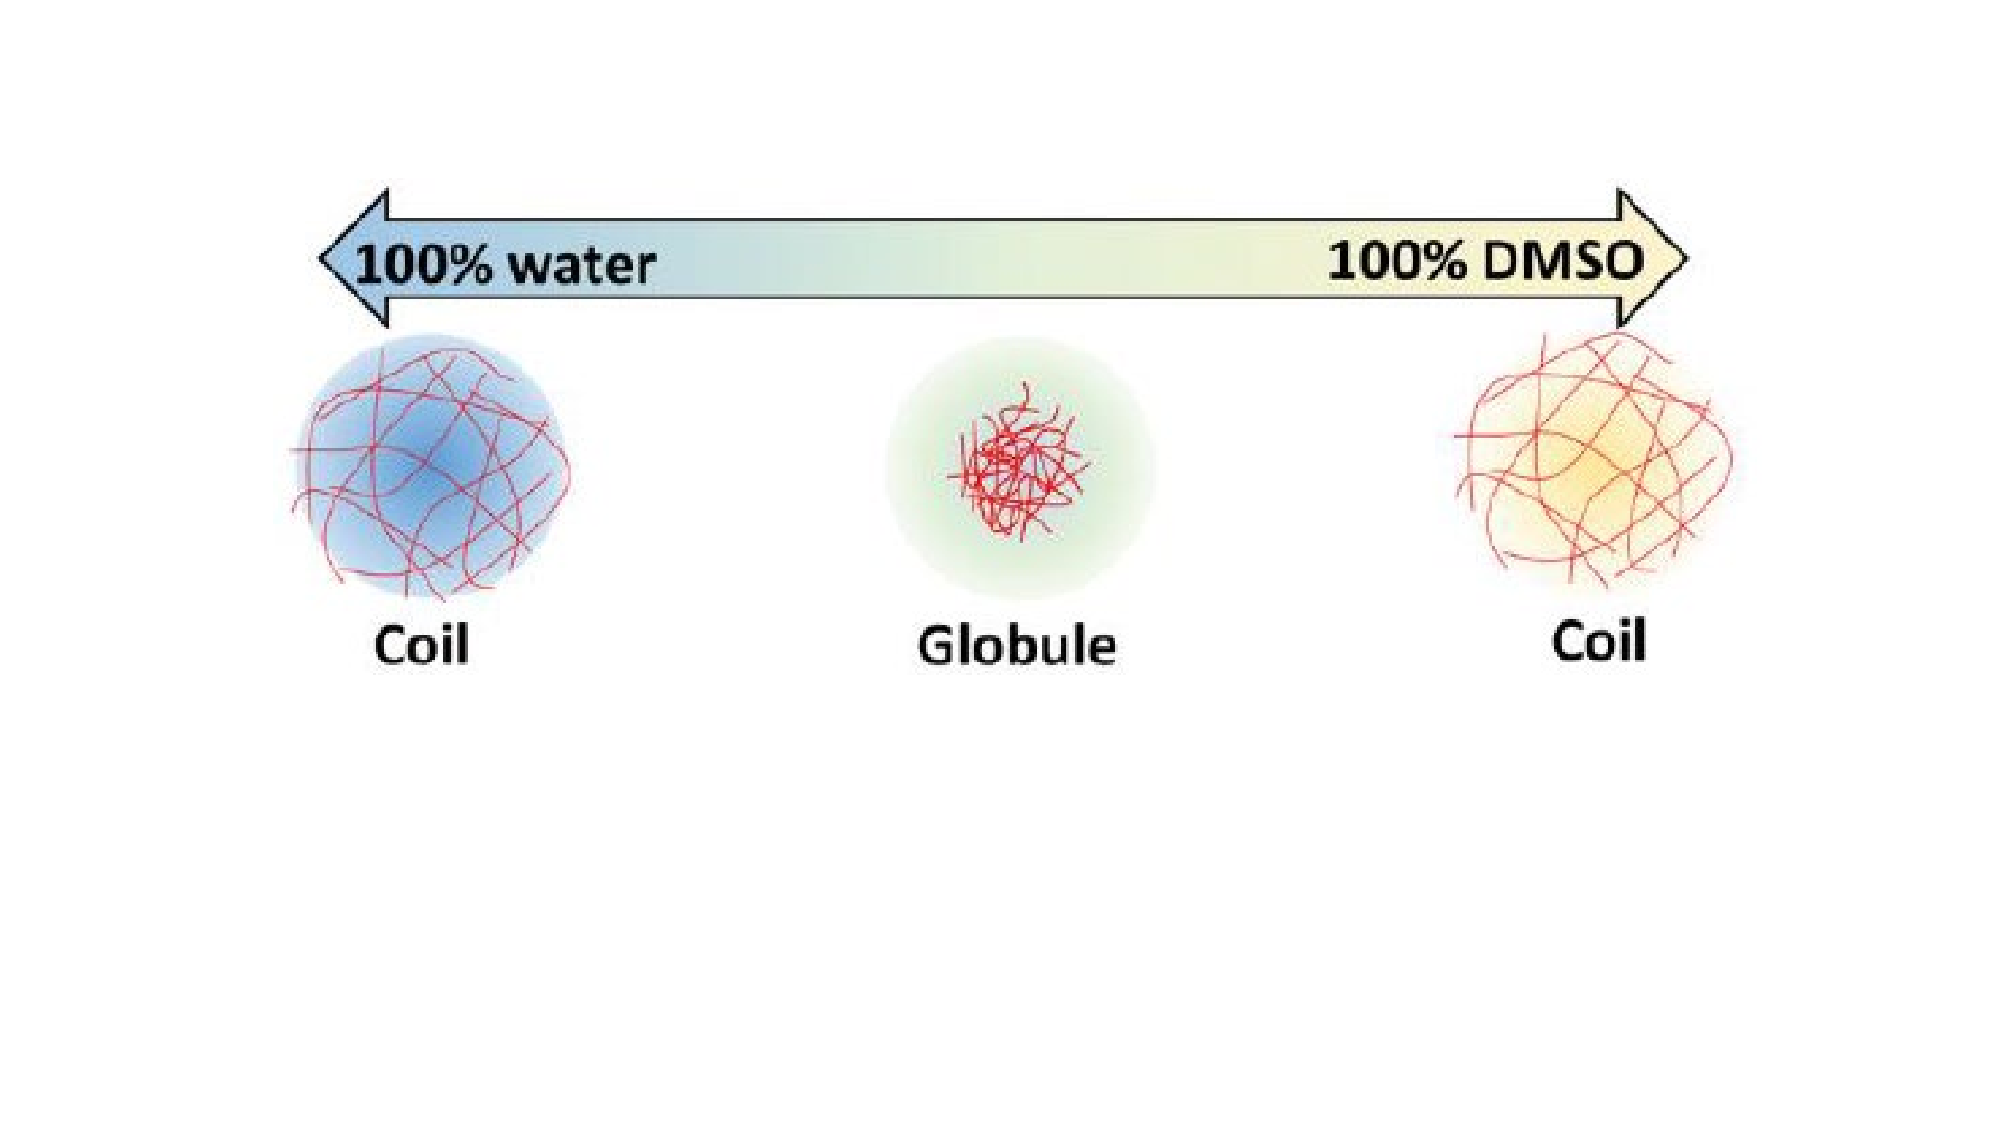
\includegraphics[width=0.7\textwidth]{cononsolv.pdf}
    \caption[]{}
    \label{fig:cononsolv}
\end{figure}

In addition, a 3D printing technique has been demonstrated. A sample 3D printed structure is shown in Figure~\ref{fig:3Dprint}. The results of this research has been accepted for publication in Advanced Materials Journal. Future work will focus on 3D printing of voxels with embedded soft heaters to remove the rigid components from the voxels and increase their production rate.
\begin{figure}[!ht]
\centering
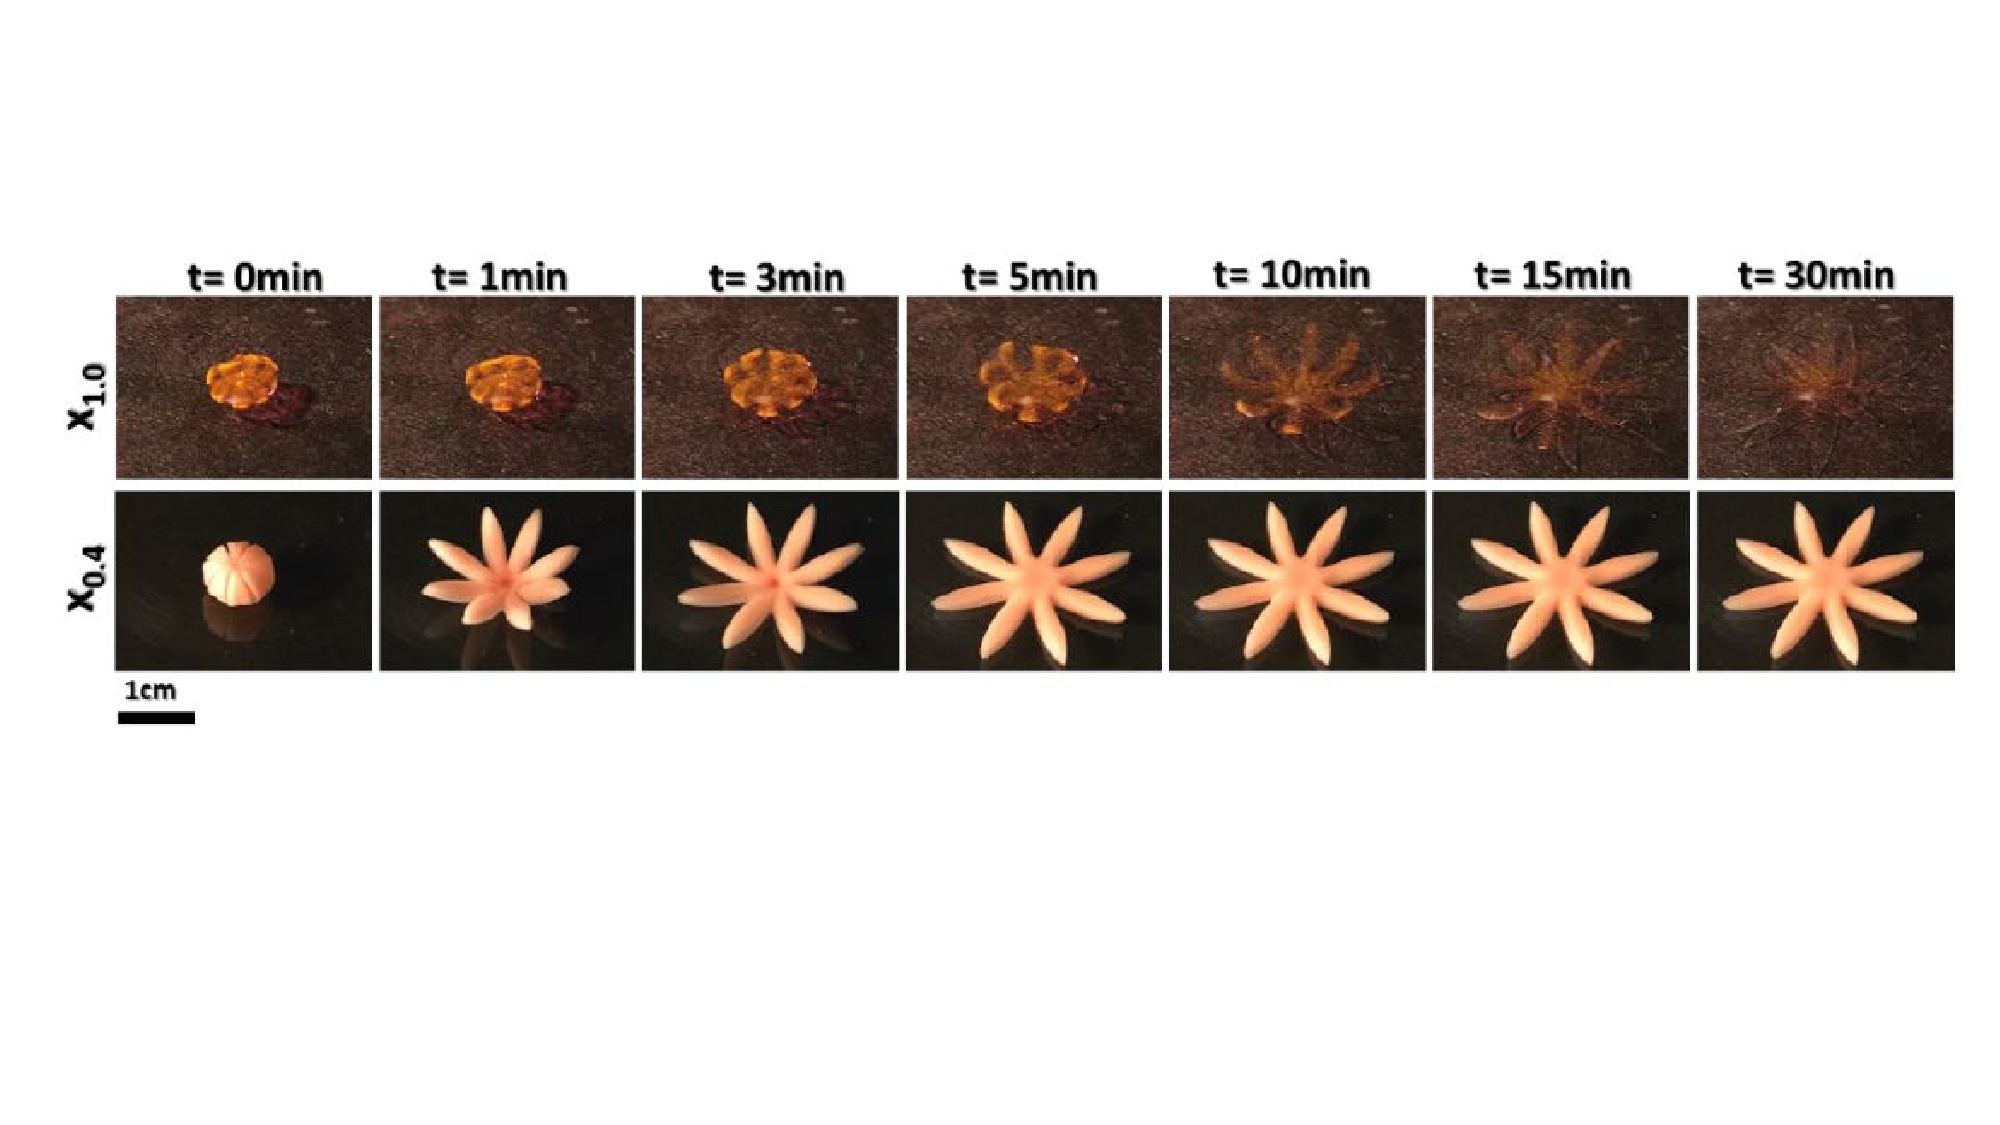
\includegraphics[width=\textwidth]{3Dprint.pdf}
    \caption[]{}
    \label{fig:3Dprint}
\end{figure}

\subsection{Control of the Hyper-redundant Robotic Arm}
\begin{figure}[!t]
\centering
\includegraphics[width=0.7\textwidth]{control.pdf}
    \caption[]{}
    \label{fig:control}
\end{figure}

\subsection{Finite Element Modeling of the Hydrogel Structures}
\begin{figure}[!t]
\centering
\includegraphics[width=0.7\textwidth]{FEM.pdf}
    \caption[]{}
    \label{fig:FEM}
\end{figure}

\subsection{Dynamic Simulation of the Voxel-based Robots}
\begin{figure}[!t]
\centering
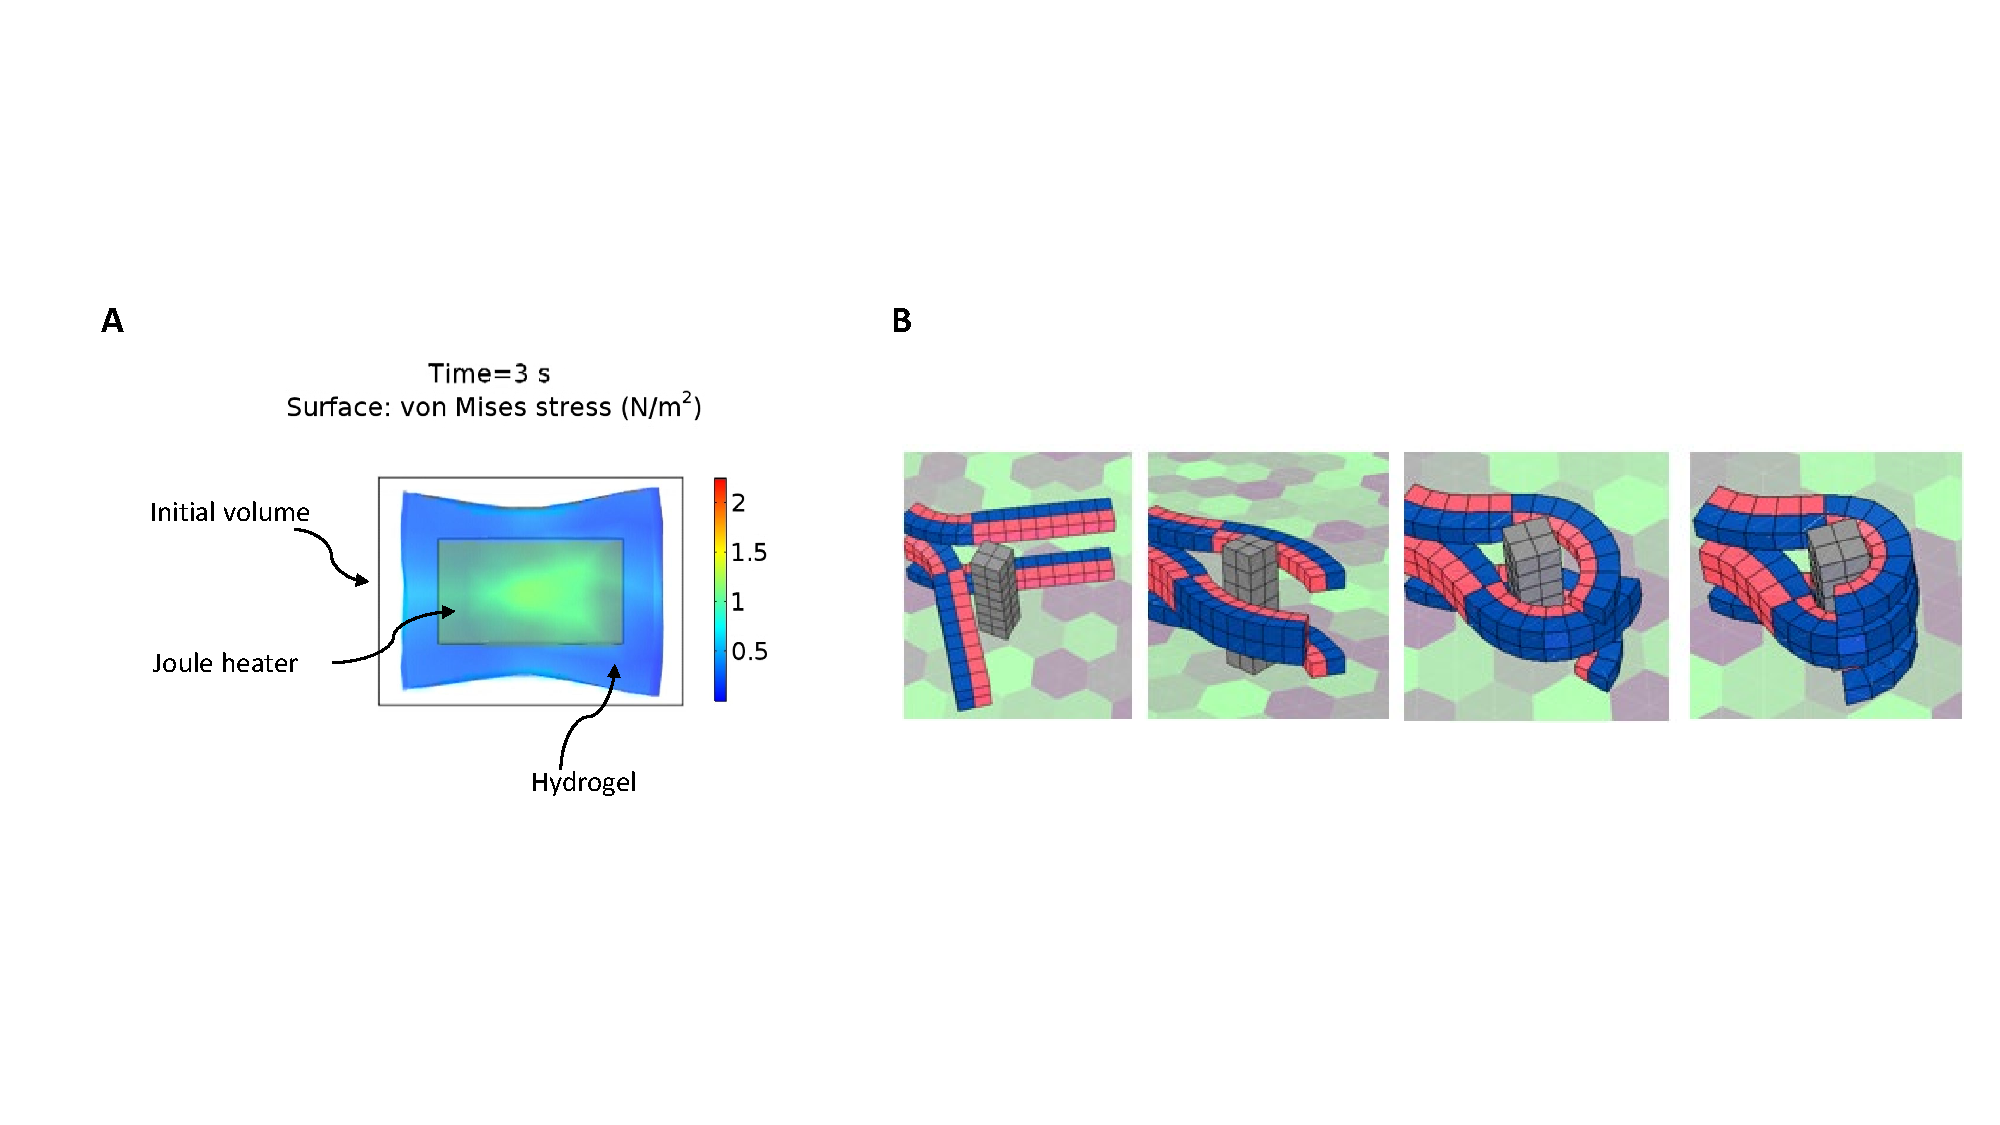
\includegraphics[width=0.7\textwidth]{voxcad.pdf}
    \caption[]{}
    \label{fig:voxcad}
\end{figure}

\subsection{A 3-dimensional prototype of the hyper-redundant robot}
\begin{figure}[!t]
\centering
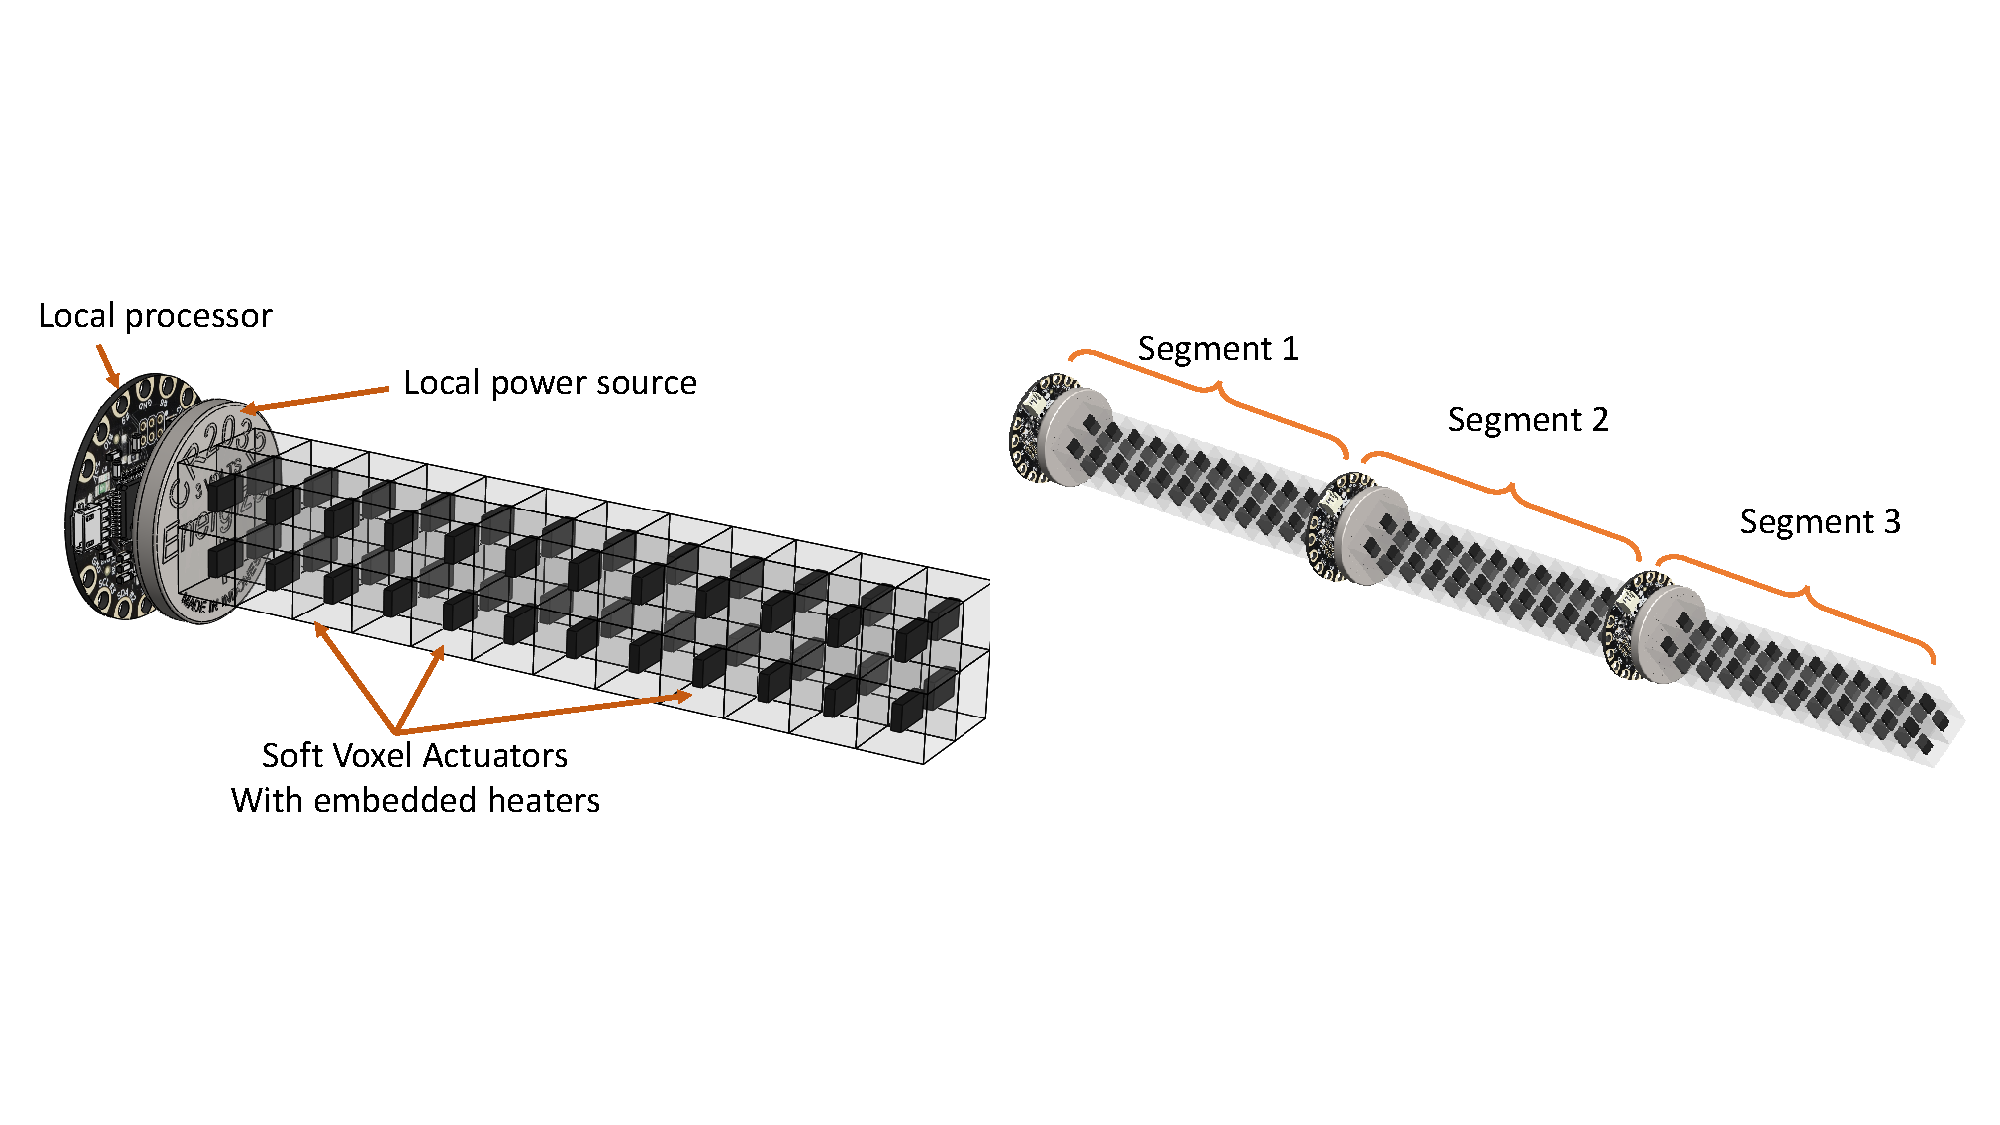
\includegraphics[width=0.7\textwidth]{3Darm.pdf}
    \caption[]{}
    \label{fig:3Darm}
\end{figure}

\subsection{Expanding the Functionality of the Robots}
\begin{figure}[!t]
\centering
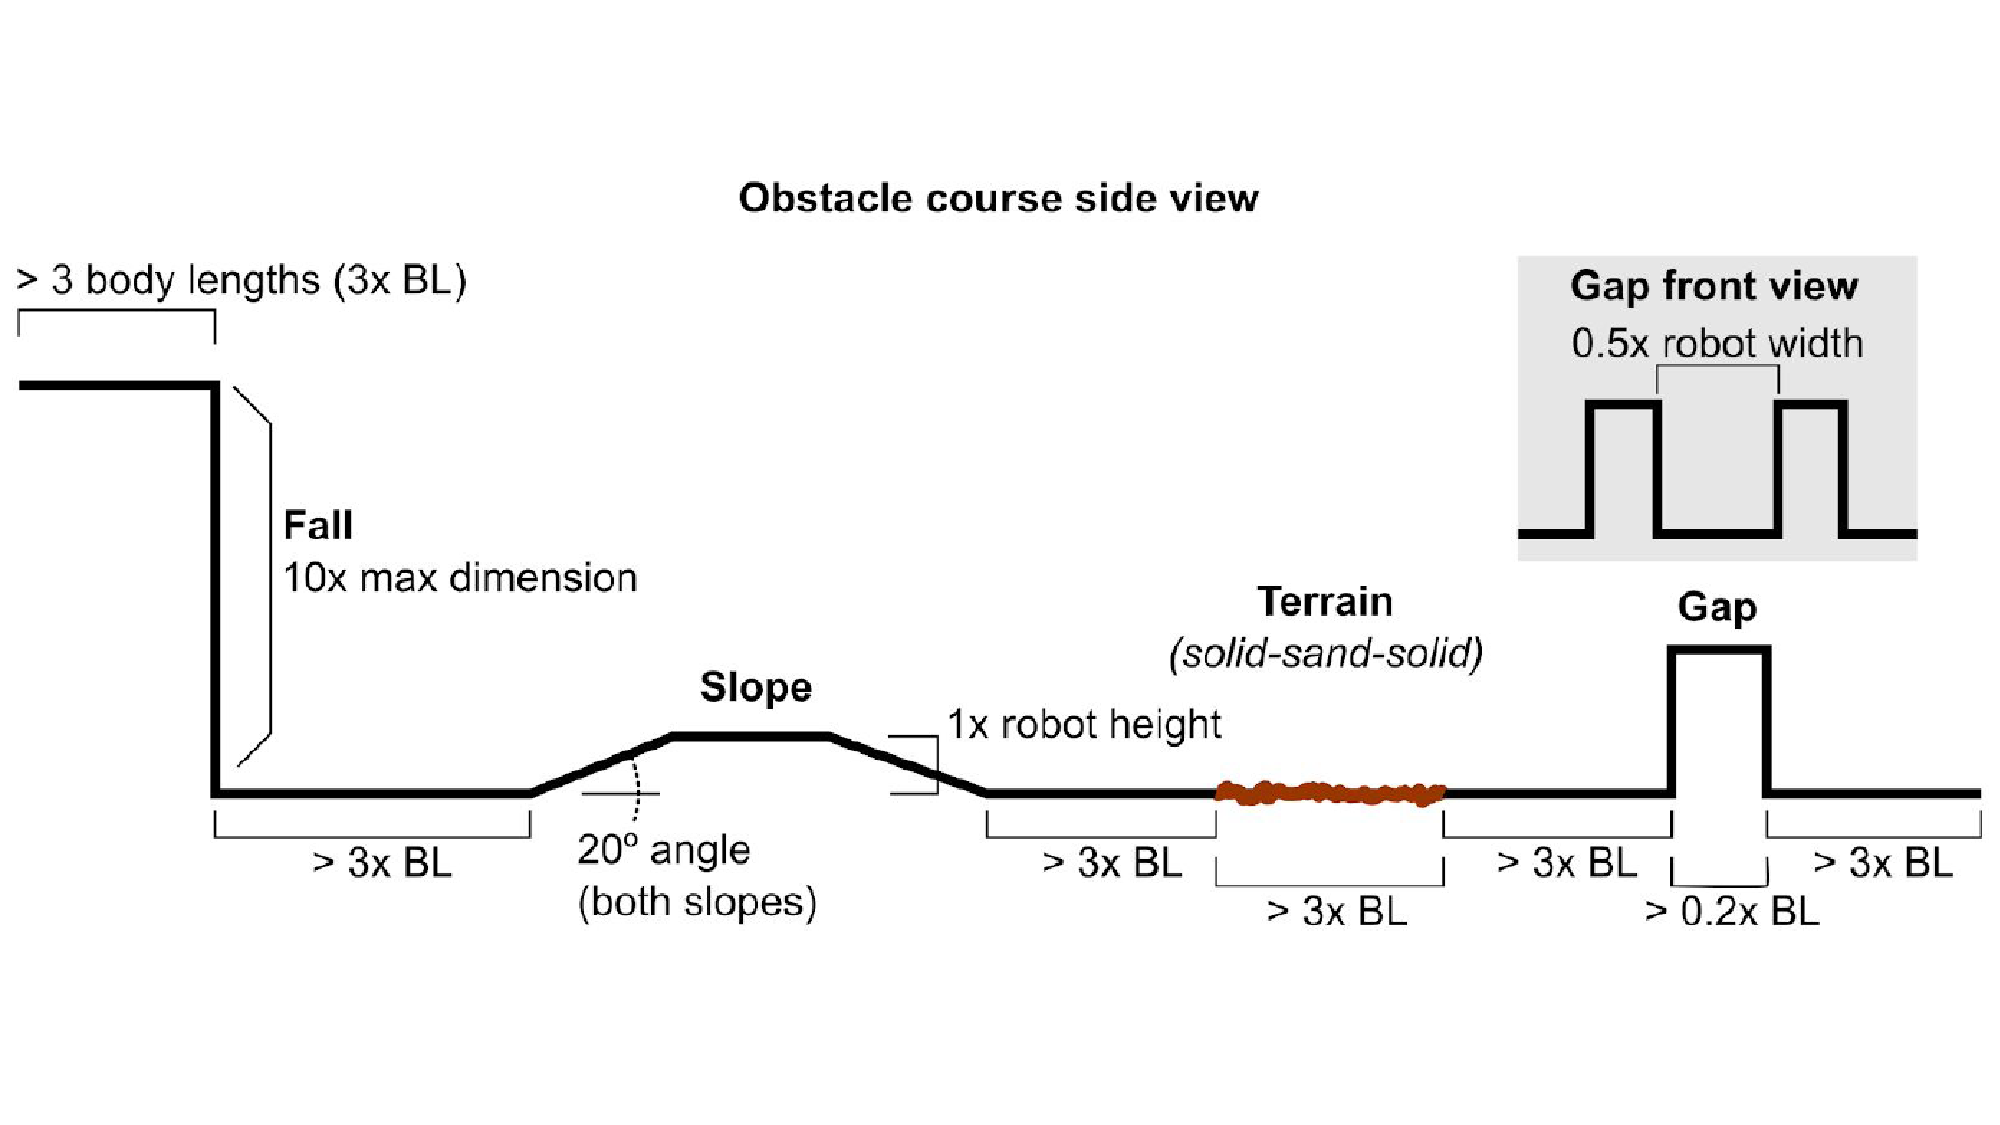
\includegraphics[width=0.7\textwidth]{sorocomp.pdf}
    \caption[]{}
    \label{fig:sorocomp}
\end{figure}

%\chapter{7}}


%-----------------------back matter
{\singlespace
% Making the references a "part" rather than a chapter gets it indented at
% level -1 according to the chart: top of page 4 of the document at
% ftp://tug.ctan.org/pub/tex-archive/macros/latex/contrib/tocloft/tocloft.pdf
\addcontentsline{toc}{part}{REFERENCES}
\bibliographystyle{ieeetran}
%\bibliography{C:/Users/rkhodamb/Documents/library}}
\bibliography{library}}

%\bibliography{allTogether}}
\renewcommand{\chaptername}{APPENDIX}
\addtocontents{toc}{APPENDIX \par}
\appendix
\doublespace
\graphicspath{{Images/control/}}

\chapter{Tracking Control of a Miniature 2-DOF Manipulator with Hydrogel Actuators}
\label{chap:control}
Due to the nature of the complex spatiotemporal dynamics of stimuli-responsive soft materials, closed-loop control of hydrogel-actuated mechanisms has remained a challenge. This paper demonstrates, for the first time, closed-loop trajectory tracking control in real-time of a millimeter-scale, two degree-of-freedom manipulator via \emph{independently-controllable}, temperature-responsive hydrogel actuators. A linear state-space model of the manipulator is developed from input-output measurement data, enabling the straightforward application of control techniques to the system. The Normalized Mean Absolute Error~(NMAE) between the modeled and measured displacement of the manipulator's tip is below 10\%. We propose an Observer-based controller and a robust $H_{\infty}$-optimal controller and evaluate their 
% stability and convergence properties. The controllers' 
performance in a trajectory tracking output-feedback framework, compared with and without sinusoidal disturbances and noise. We demonstrate in simulation that the $H_\infty$-optimal controller, which is computed using Linear Matrix Inequality (LMI) methods, tracks an elliptical trajectory more accurately than the Observer controller and is more robust to disturbances and noise. We also show experimentally that the $H_\infty$-optimal controller can be used to track different trajectories with an NMAE below 15$\%$, even when the manipulator is subject to a 3\,g load, 12.5 times an actuator's weight. Finally, a payload transport scenario is presented as an exemplar application; we demonstrate that an array of four manipulators is capable of moving a payload horizontally by applying the proposed $H_\infty$-optimal trajectory-tracking controller to each manipulator in a decoupled manner.
\section{\capitalisewords{Background}}
Soft actuators, composed of deformable matter such as fluids, gels, elastomers, and shape memory alloys (SMAs)~\cite{Majidi2014}, are lightweight and noiseless, in contrast to pneumatic systems with pumps and motors. Stimuli-responsive materials have potential applications in micro-manipulation, sensing, optics~\cite{Mantha2019,Qin2019}, and biomedical applications~\cite{Guiseppi-Elie2010}. Hydrogels in particular have the ability to absorb and release water, undergoing reversible volumetric changes that facilitates their use as soft actuators~\cite{Mishra2020}. A variety of hydrogel formulations exist, enabling these materials to change state under different external physical or chemical stimuli~\cite{Peng2018,He2012}. For example, poly(N-isopropylacrylamide), or PNIPAAM, is a commonly used temperature-responsive hydrogel that contracts when heated.

\begin{figure}[h]
\centering
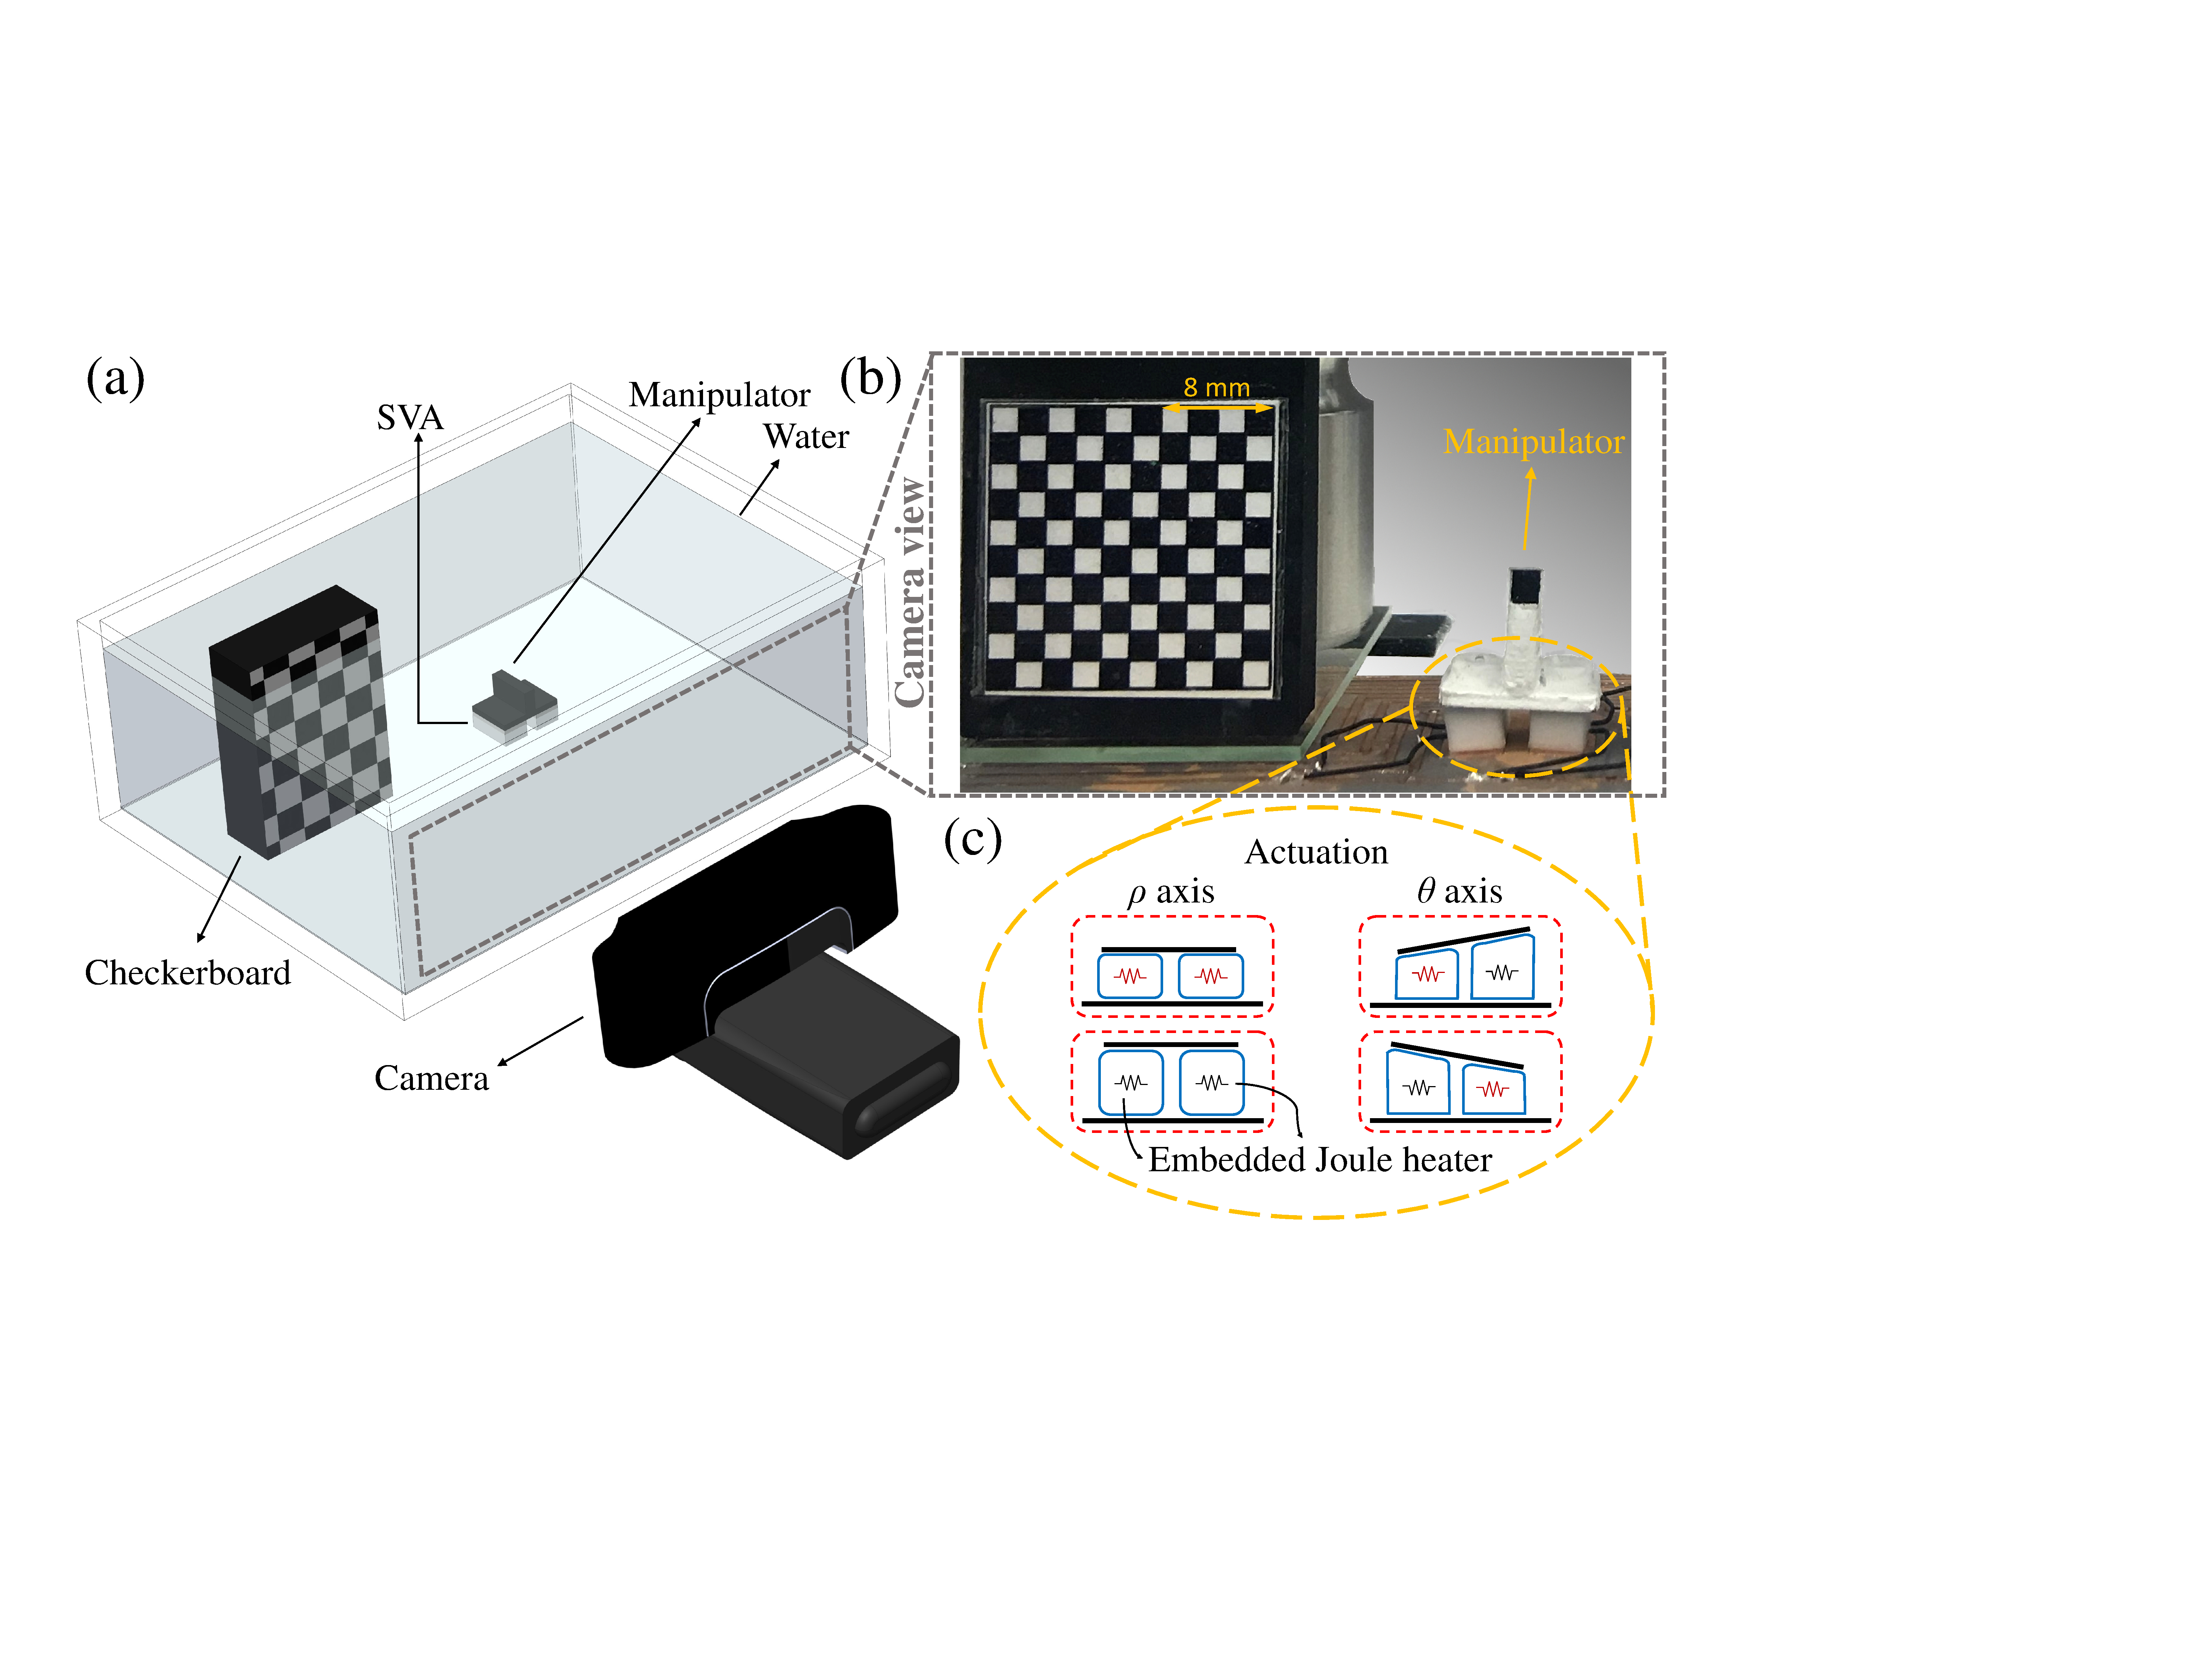
\includegraphics[width=\textwidth]{ConceptDesign6_O.pdf}
    \caption[\capitalisewords{Experimental setup for tracking control of a 2-DOF manipulator}]{Experimental setup for tracking control of a 2-DOF manipulator with embedded hydrogel Soft Voxel Actuators (SVAs)~\cite{Doroudchi2020}. (a) Illustration of a manipulator in a water-filled tank with a camera for vision-based feedback of the manipulator tip. (b) Camera view of the setup, including a fabricated 
    manipulator prototype and checkerboard for camera calibration. (c) Illustration of SVA deformation in various activation states (red = on; black = off).}
    \vspace{-0.75cm}
    \label{fig:setup}
\end{figure}

Hydrogel-based active mechanisms using morphing or bending beams and sheets have been utilized for sensing, smart micro-fluidic valves, optical lensing, and micro-scale swimming and walking~\cite{Ionov2014}. More complicated tasks, such as picking and placing objects with open-loop control methods, have also been demonstrated~\cite{Wang2015b}. Due to the nature of the stimuli, closed-loop control of hydrogel actuators has remained a challenge. Light sources such as lasers~\cite{Luo2015}, for instance, require sophisticated and bulky equipment to produce motion. The methods used in~\cite{Kim2015a} require bulk heating of the surrounding fluids, which limits their application to confined environments, such as tanks. Electric fields~\cite{Morales2014} and  chemical gradients~\cite{Du2019, Nguyen2017} affect an entire region simultaneously, which means that all actuators placed in these fields are subject to the same stimulus. This results in primitive systems that are capable of performing  simple tasks. For instance, novel devices with soft, 3D-printed, parallel, contactless actuators for biomedical applications like cell manipulation and drug release~\cite{Zolfagharian2018} use electro-responsive hydrogels and are stimulated via electric field; the actuators are simultaneously affected by changes in the electric field, resulting in a single controllable degree of actuation for the device. To enable independent actuation of multiple hydrogel actuators, we recently developed a novel approach or fabricating and integrating Soft Voxel Actuators (SVAs) composed of temperature-responsive hydrogel~\cite{Khodambashi2021}. We also presented a dynamic model for a continuum robotic arm with distributed SVAs and validated the model with open-loop control of independently actuated SVAs~\cite{Doroudchi2020}.  

In this chapter, we introduce the design, implementation, and experimental validation of {\it closed-loop controllers} for hydrogel-actuated robots. We demonstrate our control approach on a millimeter-scale, two degree-of-freedom (DOF) manipulator actuated by two SVAs, shown in Fig.~\ref{fig:setup}. Many prior control-oriented models developed for similar systems have been governed by the kinematic equations describing rigid links~\cite{Webster2010,RezayatSorkhabadi2019}, which are less useful in the design of feedback controllers for continuously deformable robots with soft actuators embedded within their structure. To address this, we propose a black-box identified model as in~\cite{Ljung2010,Schaller2020} that simplifies system dynamics in the form of a linear state-space representation. Modern control is built upon state-space models and state-space system identification, which  makes modern control techniques more practical in application~\cite{Lim1998,Chinimilli2020}. We apply system identification methods to obtain a linear state-space model of the manipulator, which can be used to implement a wide range of controllers for different applications. We design an $H_{\infty}$-optimal output-feedback tracking controller~\cite{Aastrom2010},  similar to the $H_{\infty}$ output-feedback controller in~\cite{Farhamfard2016} for flexible needles guidance with a difference that their control system is dynamic rather than static. We then compare it in simulation to an observer-based output-feedback controller. The $H_{\infty}$-optimal controller is then experimentally validated for planar reference trajectories. Finally, we show that our approach can be used to control more complex mechanisms actuated by SVAs through a demonstration of payload transport by four manipulators.

%%-----------------contribution-----------------------------
In summary, the contributions of this paper are as follows:

\begin{enumerate}
    \item Implementation of active temperature-responsive hydrogel-based actuators (the SVA) as \textbf{independently-controllable} units. 
   \item Development and experimental identification of a linear state-space model of the manipulator that can be used to implement a variety of control techniques. This linear model is sufficiently accurate for control purposes, despite the complex nonlinear dynamics of the actuators.
    \item Demonstration of, for the first time, the ability to control a 2-DOF mechanism with \textbf{independently-controllable} hydrogel actuators in real time using output-feedback controllers. 
    \item Demonstration of an exemplar payload transport application using an array of four manipulators with this versatile and computationally-inexpensive technique.
\end{enumerate}

\section{\capitalisewords{Manipulator Fabrication}}

SVAs are fabricated by embedding small Joule heaters within a mold, temperature-responsive PNIPAAM hydrogel in the shape of a rectangular prism, as illustrated in Fig.~\ref{fig:setup}b and~\ref{fig:setup}c. When an electric potential is applied across the embedded Joule heater, the actuator shrinks uniformly. The manipulator, also shown in Fig.~\ref{fig:setup}b, consists of two SVAs affixed to a 3D-printed T-shaped extension, which serves as the end-effector. A standard PNIPAAM hydrogel precursor solution is used to fabricate the SVAs from thermo-responsive hydrogel, using a recipe described in~\cite{Khodambashi2021}. Each SVA is $8\times4.5\times3$\,mm$^3$ in its fully swollen state, with a total weight of 0.12\,g, including the embedded-Joule heater (10\,$\Omega$ SMD resistor 0805), which is connected to microcontrollers by wires. The T-shaped extension is 3D-printed in nylon using a Markforged M2 3D printer. 
A circuit board, which serves as the fixed base of the manipulator, is attached to one side of the two SVAs; the T-shaped extension is attached to the other side. The circuit board and extension are attached to the SVAs with superglue to ensure that they remain in contact with the SVAs during the experiments. Since hydrogels must be immersed in water to absorb water when cooling, all experiments are conducted in a tank of deionized (DI), room-temperature water.

\section{\capitalisewords{Experimental Setup}}

% \spr{(Some of the text in this section was changed from the original version. The new text should be highlighted in blue.)}\rke{Roozbeh would you please compare with the original paper and apply Spring's comment? thanks, Azadeh}
Figure~\ref{fig:setup} shows the experimental setup used for closed-loop control and tracking of the manipulator's trajectory. A Logitech C930e USB Webcam is placed in front of the tank to send real-time data to the image processing program in MATLAB which tracks the position of a marker on the manipulator tip. These measurements of the manipulator tip's position over time are transmitted back to the controller. We used a black-and-white checkerboard with 2~mm $\times$ 2~mm squares to estimate the camera calibration factors (mm/pixel) along the $x$ and $y$ axis (Fig.~\ref{fig:setup}). White was selected as the color of the tank's background, and black was selected as the color of the manipulator tip's marker to facilitate contrast-based filtering between the foreground and background. The Camera Calibration Toolbox in MATLAB was initially used to compensate for lens distortion, but since this increased the image processing time by 30\% without significantly improving the image data, the original camera images were subsequently used without compensation. All control algorithms are implemented in MATLAB; the controller output is sent to an Arduino Mega2560, which acts as the physical communication layer between MATLAB and a  PCA9685 MOSFET board. This MOSFET board, with 16 discrete output channels, receives a PWM signal from the controller and applies it (maximum: 3.7\,V) at higher current to the corresponding Joule heater.

\section{\capitalisewords{Manipulator Modeling}}

In this section, the kinematics of the manipulator are derived in order to compute its workspace. A two-dimensional linear state-space model of the manipulator is then defined using black-box system identification methods. 


\subsection{Kinematics and Workspace}
\begin{figure}[h]
\centering
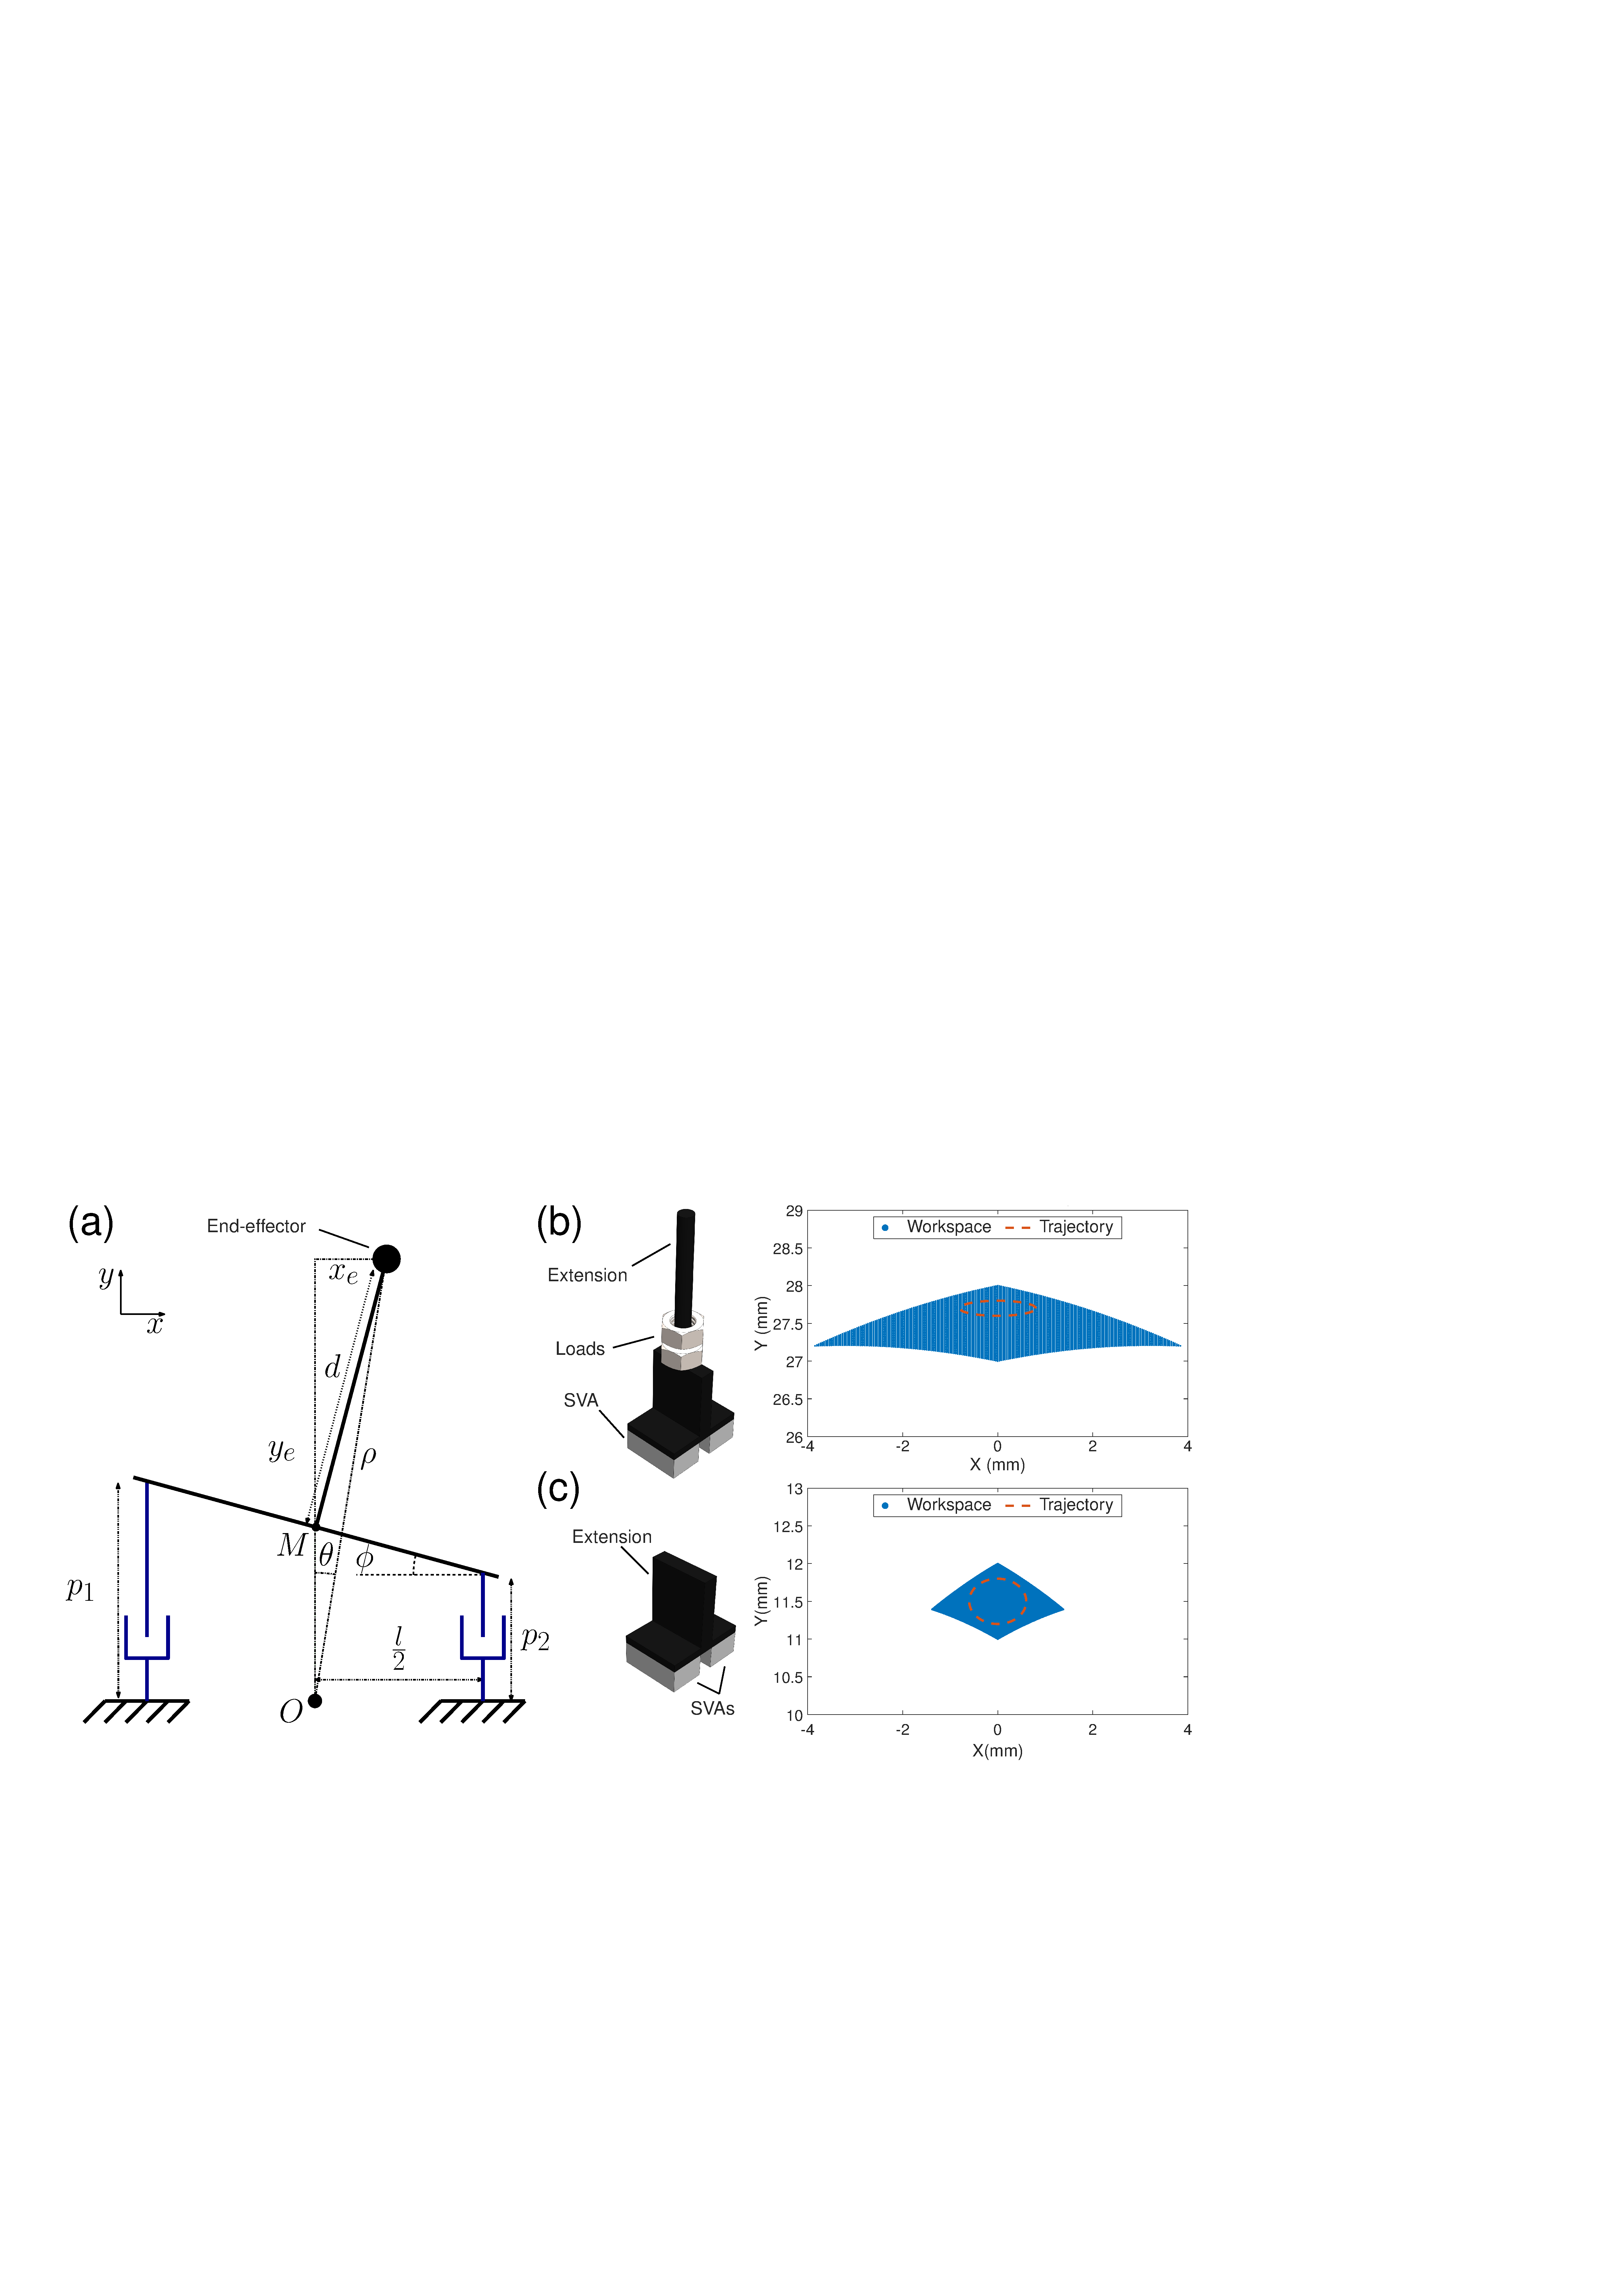
\includegraphics[width=\textwidth]{Path_Picture_New_Eleven.pdf}
    \caption[\capitalisewords{Schematic and workspace of the manipulator}]{Schematic and workspace of the manipulator. (a) The 2-DOF parallel mechanism model with two prismatic joints. (b), (c) Workspaces for extensions with lengths $d=25$\,mm and $d=9$\,mm, respectively, with exemplar elliptical trajectories overlaid in red. Extra loads are added to the longer extension in (b) to test the robustness of the controller in experiment.}
    \label{fig:Path}
\end{figure}
 
To derive manipulator tip kinematics and  workspace, the SVAs are modeled as two prismatic joints, as illustrated in Fig.~\ref{fig:Path}a. The T-shaped extension is assumed to be rigid compared to the SVAs that are rigidly attached to the extension and circuit board. The SVAs are modeled as linear contractile elements since only one dimension of their volumetric shape change influences the displacement of the manipulator. Thus, with two prismatic actuators connected in parallel, the manipulator may be considered a 2-DOF mechanism. As shown in Fig.~\ref{fig:Path}a, we define $p_1$ and $p_2$ as the linear displacement of each SVA. These values vary between 3\,mm in inactivated SVA to 2\,mm when activated by the embedded Joule heaters;
$l=$6.5\,mm is the spacing between SVAs, $d$ is the length of the extension, and $\phi$ shows the extension's angle from the horizontal axis. We assume point $M$'s displacement in the $x$ direction is negligible~(Fig.~\ref{fig:Path}a).  The forward kinematics of the manipulator may be computed geometrically for the manipulator tip's, $\vect{p}_e$, in Cartesian coordinates, $x_e$ and $y_e$, in the reference frame with origin $O$, according to
%\dma{WHY ALL THE VSPACES?  THE TEMPLATE SPECIFIES THE SPACING.}]\azy{I assume they are from the shortened version-6 pages one}
\begin{align}
\vect{p_e}  &= \begin{bmatrix}x_e & y_e\end{bmatrix}^T,~~\phi = \arctan(\dfrac{p_1-p_2}{l}),\\
x_e &= d \sin(\phi),~~y_e= d \cos(\phi) + \dfrac{p_1+p_2}{2}.
\end{align}
The polar coordinates $\rho$ and $\theta$ of the manipulator's tip in this reference frame (see Fig.~\ref{fig:Path}a) are given by  

\begin{align}
\rho &=  \sqrt{x_e^2 + y_e^2},~~\theta = \arctan \left(\dfrac{x_e}{y_e}\right).
\end{align}
 
As illustrated in Fig.~\ref{fig:setup}c, if both SVAs are activated simultaneously with the same input voltage, then the manipulator's tip moves along the $\rho$-axis at a constant $\theta$; if only the left or right SVA is activated, then the tip undergoes an angular displacement at a constant $\rho$. Other SVA activation patterns produce a combination of displacements in both $\rho$ and $\theta$. 
% The SVAs used in this work have initial displacements of $p_1 = p_2 = 3$\,mm, and they have a maximum contraction of $p_1 = p_2 =$ 2\,mm when activated by the embedded Joule heaters. \dma{REVIEW TO SHORTEN}The spacing between them is $l =$ 6.5\,mm.
Two different extensions with lengths of $d = 25$\,mm and $d=9$\,mm were fabricated and tested, and their workspaces are shown in  Figs.~\ref{fig:Path}b and c, respectively. The longer extension is used to amplify the motion of each actuator, resulting in a larger workspace and making the controller performance easier to measure and evaluate. Extra loads may be added to the shaft of the longer extension, as shown in the left image in Fig.~\ref{fig:Path}b, in order to experimentally test the robustness of the controller. The shorter extension, by contrast, supports higher loads on the tip during trajectory tracking, as demonstrated in the payload transport application in Section \ref{sec:payload}.


\subsection{Linear State-Space Model}

As explained in the last section, the displacements of the SVAs and manipulator tip are not decoupled, since the T-shaped extension connecting the actuators to the tip establishes a rigid kinematic transformation from the prismatic motion of the actuators to the 2-DOF planar motion of the end-effector.
% Thus, the manipulator is similarly modeled as a multivariable control system with two inputs and two outputs, where the inputs are the voltages applied to the SVAs ($V_1$, $V_2$) and the outputs are the tip's position in polar coordinates ($\rho$, $\theta$). 
We model this control system using a two-dimensional linear state-space representation, which enables the implementation of a variety of control methods. Defining $\vect{x}(t) \in \mathbb{R}^{4\times1}$ as the vector of unknown system state variables at time $t$, $\dot{\vect{x}}(t)$ as the vector of time derivatives of the state variables, %as the derivative of the states with respect to time, 
$\vect{u}(t)=[V_1(t) \quad V_2(t)]^T$ as the vector of inputs, and $\vect{y}(t)=[\theta(t) \quad \rho(t)]^T$ as the vector of outputs, the state-space model is given by
% \dma{ISN'T THIS STANDARD?} \spr{yes, but we refer to this model later}
\begin{align}
\dot{\vect{x}}(t)&= \vect{A}\vect{x}(t)+\vect{B}\vect{u}(t), \nonumber\\
\vect{y}(t)&= \vect{C}\vect{x}(t)+\vect{D}\vect{u}(t)\label{eq:2Dmodel} 
\end{align}
where the matrices $\vect{A}$, $\vect{B}$, $\vect{C}$, and $\vect{D}$ must be determined for each extension (25\,mm and 9\,mm), separately. Since the state variables of the model are not necessarily measurable, it is crucial to understand the relationship between various input-output models and state-space models in order to accurately identify the state-space model from input-output data~\cite{Lim1998}. To find and select a model that best represents the system's behavior, a number of models were considered including state-space models of different dimensionalities.
% polynomial or nonlinear representations. However, since the state-space model 
the 2-input 2-output showed a good fit to the data and also directly provides the unknown matrices that are required for  designing the controller, we identified the system using a state-space model. $\vect{A}$, $\vect{B}$, $\vect{C}$, and $\vect{D}$ were identified by applying black-box system identification to a set of time series input-output data according to~\cite{Ljung2001}, using the MATLAB System Identification Toolbox. The identified matrices for the 25\,mm extension were found to be: 

\begin{align*}
\vect{A} &=\begin{bmatrix} 
   -0.0007 &  -0.0301  &  0.0444 &   6.0548\\
   -0.0016 &  -0.0623  &  0.0254 &  -1.4325\\
   -0.2613  &  0.6580  &  7.2633 &-374.9846\\
   -0.0243  &  0.1643  &  3.0590 & -44.3024
    \end{bmatrix},\\
\vect{B} &=\begin{bmatrix}
    0.0001 &   0.0003\\
   -0.0000 &  -0.0001\\
   -0.0051 &  -0.0232\\
   -0.0001 &  -0.0042\\
    \end{bmatrix},\\
\vect{C} &=\begin{bmatrix}  
 1.1446  & -0.0046  & -0.0020  &  0.0034\\
-1.1431  & -3.5368  &  0.0020 &  -0.0534
    \end{bmatrix},\\
\vect{D} &=\begin{bmatrix}
     0  &   0\\
     0  &   0
    \end{bmatrix}.
\end{align*}
 
Multiple input-output datasets were gathered across various ranges of amplitudes and frequencies to find a state-space model. Among all the input signals, the fastest signal that permitted the hydrogel actuators to respond across their full temperature range was selected as the primary modeling input. Figure~\ref{fig:sim}a plots two selected input voltages among the data set that were experimentally applied to the SVAs which covers the tip workspace and depicts a 50\%  shift in the SVAs' input signal. Since the hydrogel-based SVAs have a relatively slow response, especially during their cooling phase, they were actuated from a starting point of half-actuation (50\%) in order to improve both the speed and tracking performance of the manipulator and the signal reaches the minimum and maximum values during the cycle. Fig.~\ref{fig:sim}b displays the resulting displacement of the manipulator tip and the outputs of the identified model \eqref{eq:2Dmodel} for the same inputs. These figures, which are a comprehensive example of comparison between the actual data and the identified model output, show that the model outputs $\rho$ and $\theta$ follow the corresponding measured output values throughout the duration of the experiment, with the NMAE for $\rho$ and $\theta$ given by 0.026\,mm (5.7\%) and 0.008\,rad (6.6\%), respectively. The NMAE value remains below 10\% for other tested data sets. Thus, our linear state-space model of the entire mechanism is sufficiently accurate to use in the design of controllers for the manipulator, despite the difficult-to-characterize nonlinear dynamics of the hydrogel actuators themselves.

\begin{figure}[h]
\centering
{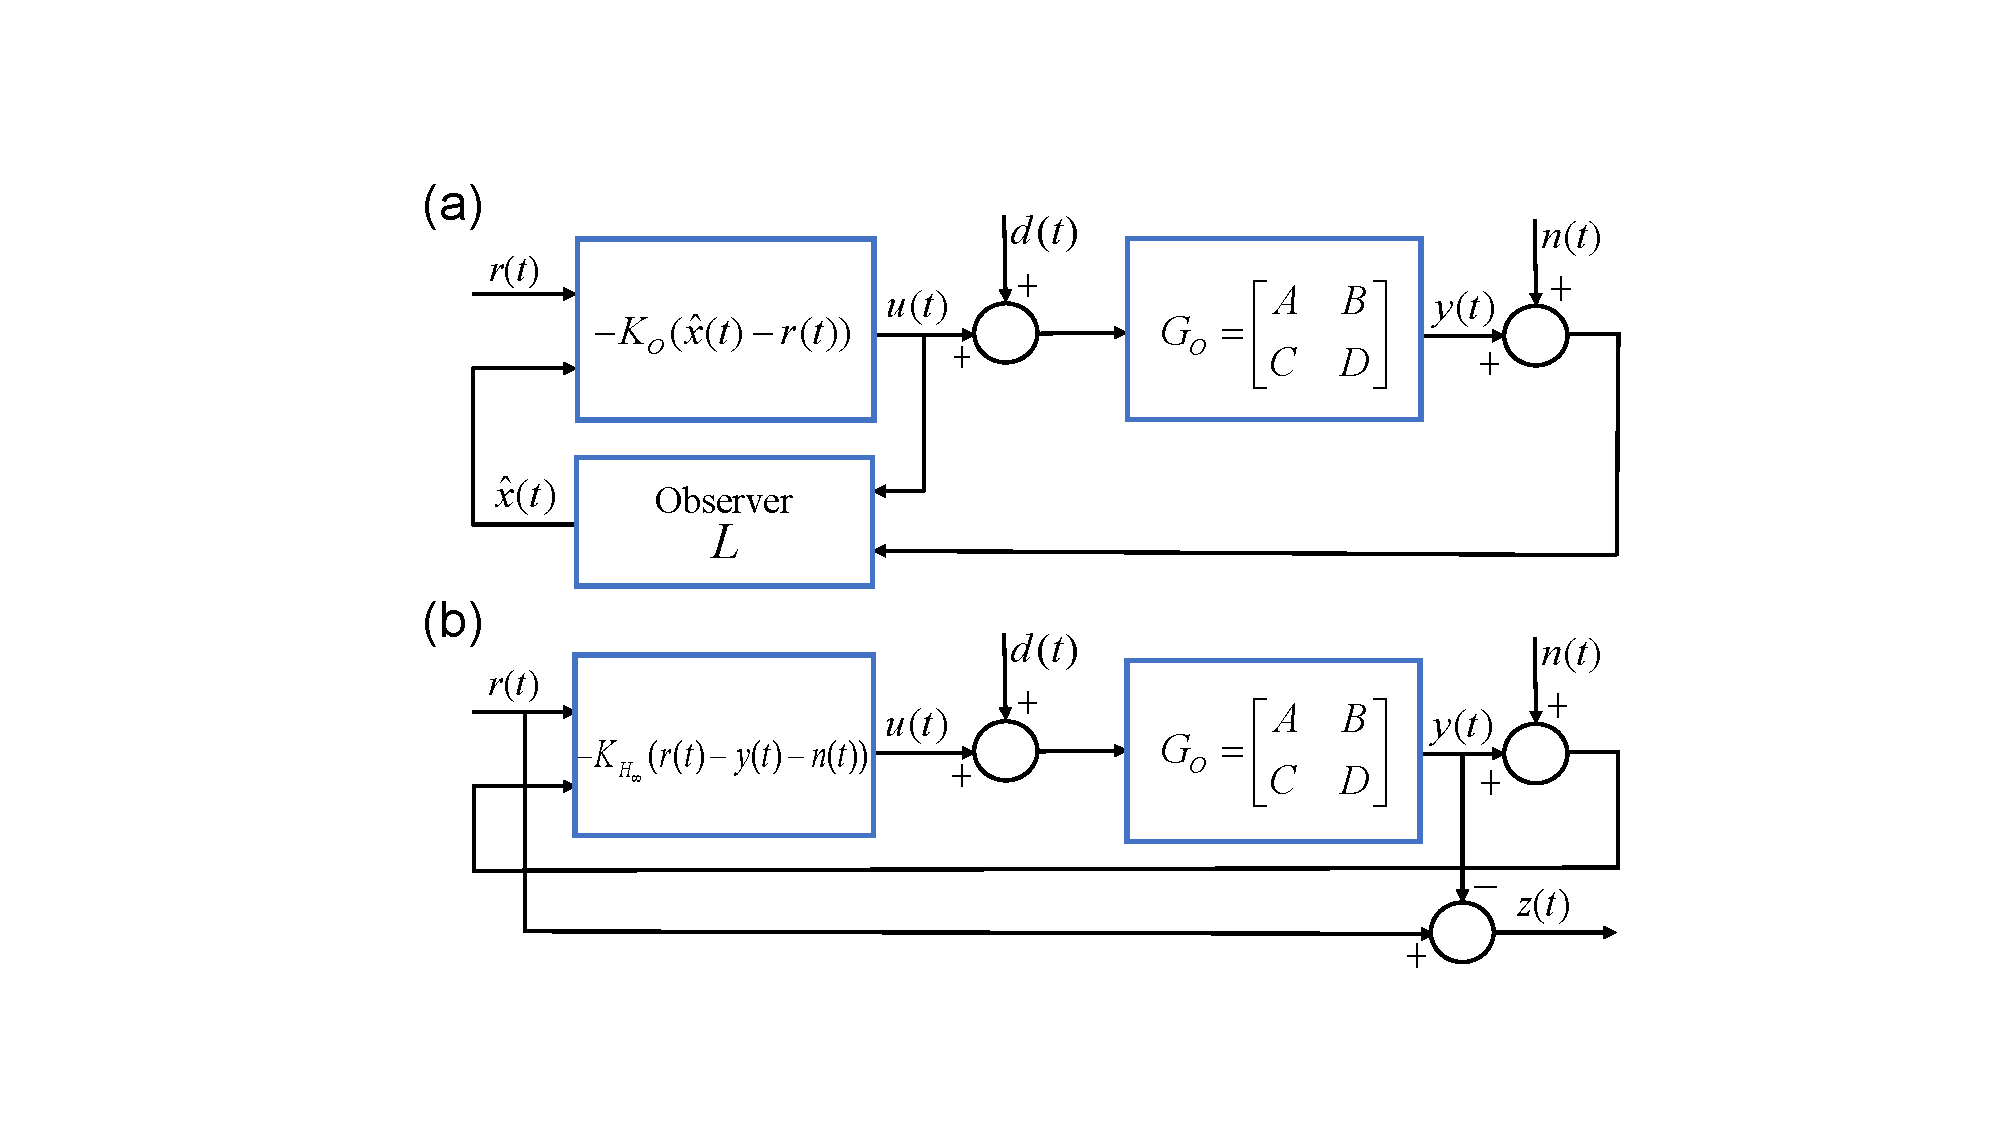
\includegraphics[width=\textwidth]{output-feedback-control_block_final.pdf}}
\caption[\capitalisewords{Block diagrams of the proposed output-feedback controllers}]{Block diagrams of the proposed output-feedback controllers with state-space representation in the tracking framework~\cite{Skogestad2007}. (a) Observer-based controller. (b) $H_\infty$-optimal controller.} \vspace{-0.5cm}
\label{fig:control_block}
\end{figure}

\section{\capitalisewords{Controller Design}} 

It can be shown that the open-loop state-space model~\eqref{eq:2Dmodel}, which has the corresponding transfer function $\vect{G}_o(s)$, is stable, controllable, and observable. In this section, we design two trajectory tracking controllers based on this state-space model, an observer-based output-feedback controller and an $H_{\infty}$-optimal output-feedback controller. Block diagrams of the controllers are illustrated in Fig.~\ref{fig:control_block}. Both controllers are designed to track a reference trajectory $\vect{r}(t) \in \mathbb{R}^{2\times1}$ while attenuating the effects of noise, denoted by $\vect{n}(t)\in \mathbb{R}^{2\times1}$, and external disturbances, denoted by $\vect{d}(t)\in \mathbb{R}^{2\times1}$.

\subsection{Observer-based output-feedback controller}

In this type of controller, an observer is designed to compute an estimate  $\hat{\vect{x}}(t)$ of the unknown system state vector $\vect{x}(t)$ from the control input $\vect{u}(t)$ and the output $\vect{y}(t)$. The control input is defined as 
\begin{align}
&\vect{u}(t)=-\vect{K}_O\left(\hat{\vect{x}}(t)-\vect{r}(t)\right), \label{eq:obs-ctl-law}
\end{align}
where $\vect{K}_O \in \mathbb{R}^{2\times4}$ is the feedback gain matrix, which can be computed as though all state variables are measurable, depending only on the $\vect{A}$ and $\vect{B}$ matrices. With this control input, the observer is given by 

\begin{align}
&\hat{\dot{\vect{x}}}(t)=(\vect{A}-\vect{B}\vect{K}_O-\vect{LC})\hat{\vect{x}}(t)+\vect{L}\vect{y}(t), \label{eq:obs-estimate}
\end{align}
where $\vect{L}\in \mathbb{R}^{4\times2}$, the observer gain matrix, must be defined such that $\vect{A-LC}$ is a Hurwitz matrix~\cite{Aastrom2010}.
The following $\vect{K}_O$ and $\vect{L}$ matrices were computed for the 25\,mm extension: 

% \spr{(should we explain how?)} \azy{I think as it is the typical observer calculations we don't need to}
\begin{align*}
\vect{K}_O &=\begin{bmatrix}  
            -3.8929  & 2.3760   &  -0.1061  &  0.2888\\
             3.6672  & -0.9670  &   0.0949  & -0.2706
    \end{bmatrix},\\
\vect{L} &=\begin{bmatrix}
           18.5160 &  -21.9676\\   
            0.1852 &  -7.7968\\
           -0.0051 &   0.0232\\
           -0.0649 &   0.0042\\
    \end{bmatrix}.
\end{align*}

\subsection{$H_\infty$-optimal output-feedback controller}

The $H_\infty$-optimal controller is designed using Linear Matrix Inequality (LMI) methods~\cite{Duan2013a,Boyd1994}; MATLAB's YALMIP toolbox~\cite{Lofberg2004} is then used to solve the optimization problem numerically. rev{The interconnected system $S(\vect{K}_{H_{\infty}},\vect{G}_o)$ of the optimal gain matrix $\vect{K}_{H_{\infty}}\in \mathbb{R}^{2\times2}$ and the open-loop system $\vect{G}_o(s)$, with external input defined as $\vect{w}=~[\vect{r}^T~\vect{d}^T~\vect{n}^T]^T \in \mathbb{R}^{6\times1}$ and external output $\vect{z}=\vect{r}-\vect{y}$, represents the closed-loop system with the ${H_{\infty}}$ gain:} \vspace{2mm}
\begin{align}
\norm{\vect{z}}_{L_2} ~\leq~ \norm{S(\vect{K}_{H_{\infty}},\vect{G}_o)}_{H_{\infty}} \norm{\vect{w}}_{L_2}.
\end{align}

The optimal gain matrix $\vect{K}_{H_{\infty}}$ is obtained as the solution to an optimization problem that minimizes the effect of the external input ($\vect{w}$) on the external output ($\vect{z}$). We can prove that the ${H_{\infty}}$ gain is bounded using the bounded-real lemma~\cite{Boyd1994}~(see Appendix). The control law is designed in the the output-feedback tracking structure: \vspace{2mm}
\begin{align}
\vect{u}(t)=-\vect{K}_{H_\infty}(\vect{r}(t)-\vect{y}(t)-\vect{n}(t)). \label{eq:Hinf-ctl}
\end{align}

The gain matrix for the 25\,mm extension %manipulator 
was computed as \vspace{2mm}
\begin{align*}
\vect{K}_{H_{\infty}} &=\begin{bmatrix}  
           -1.7371  &  2.9015 \\
           -0.3775  & -2.4158  
    \end{bmatrix}.
\end{align*}


\begin{figure*}[t]
\centering
    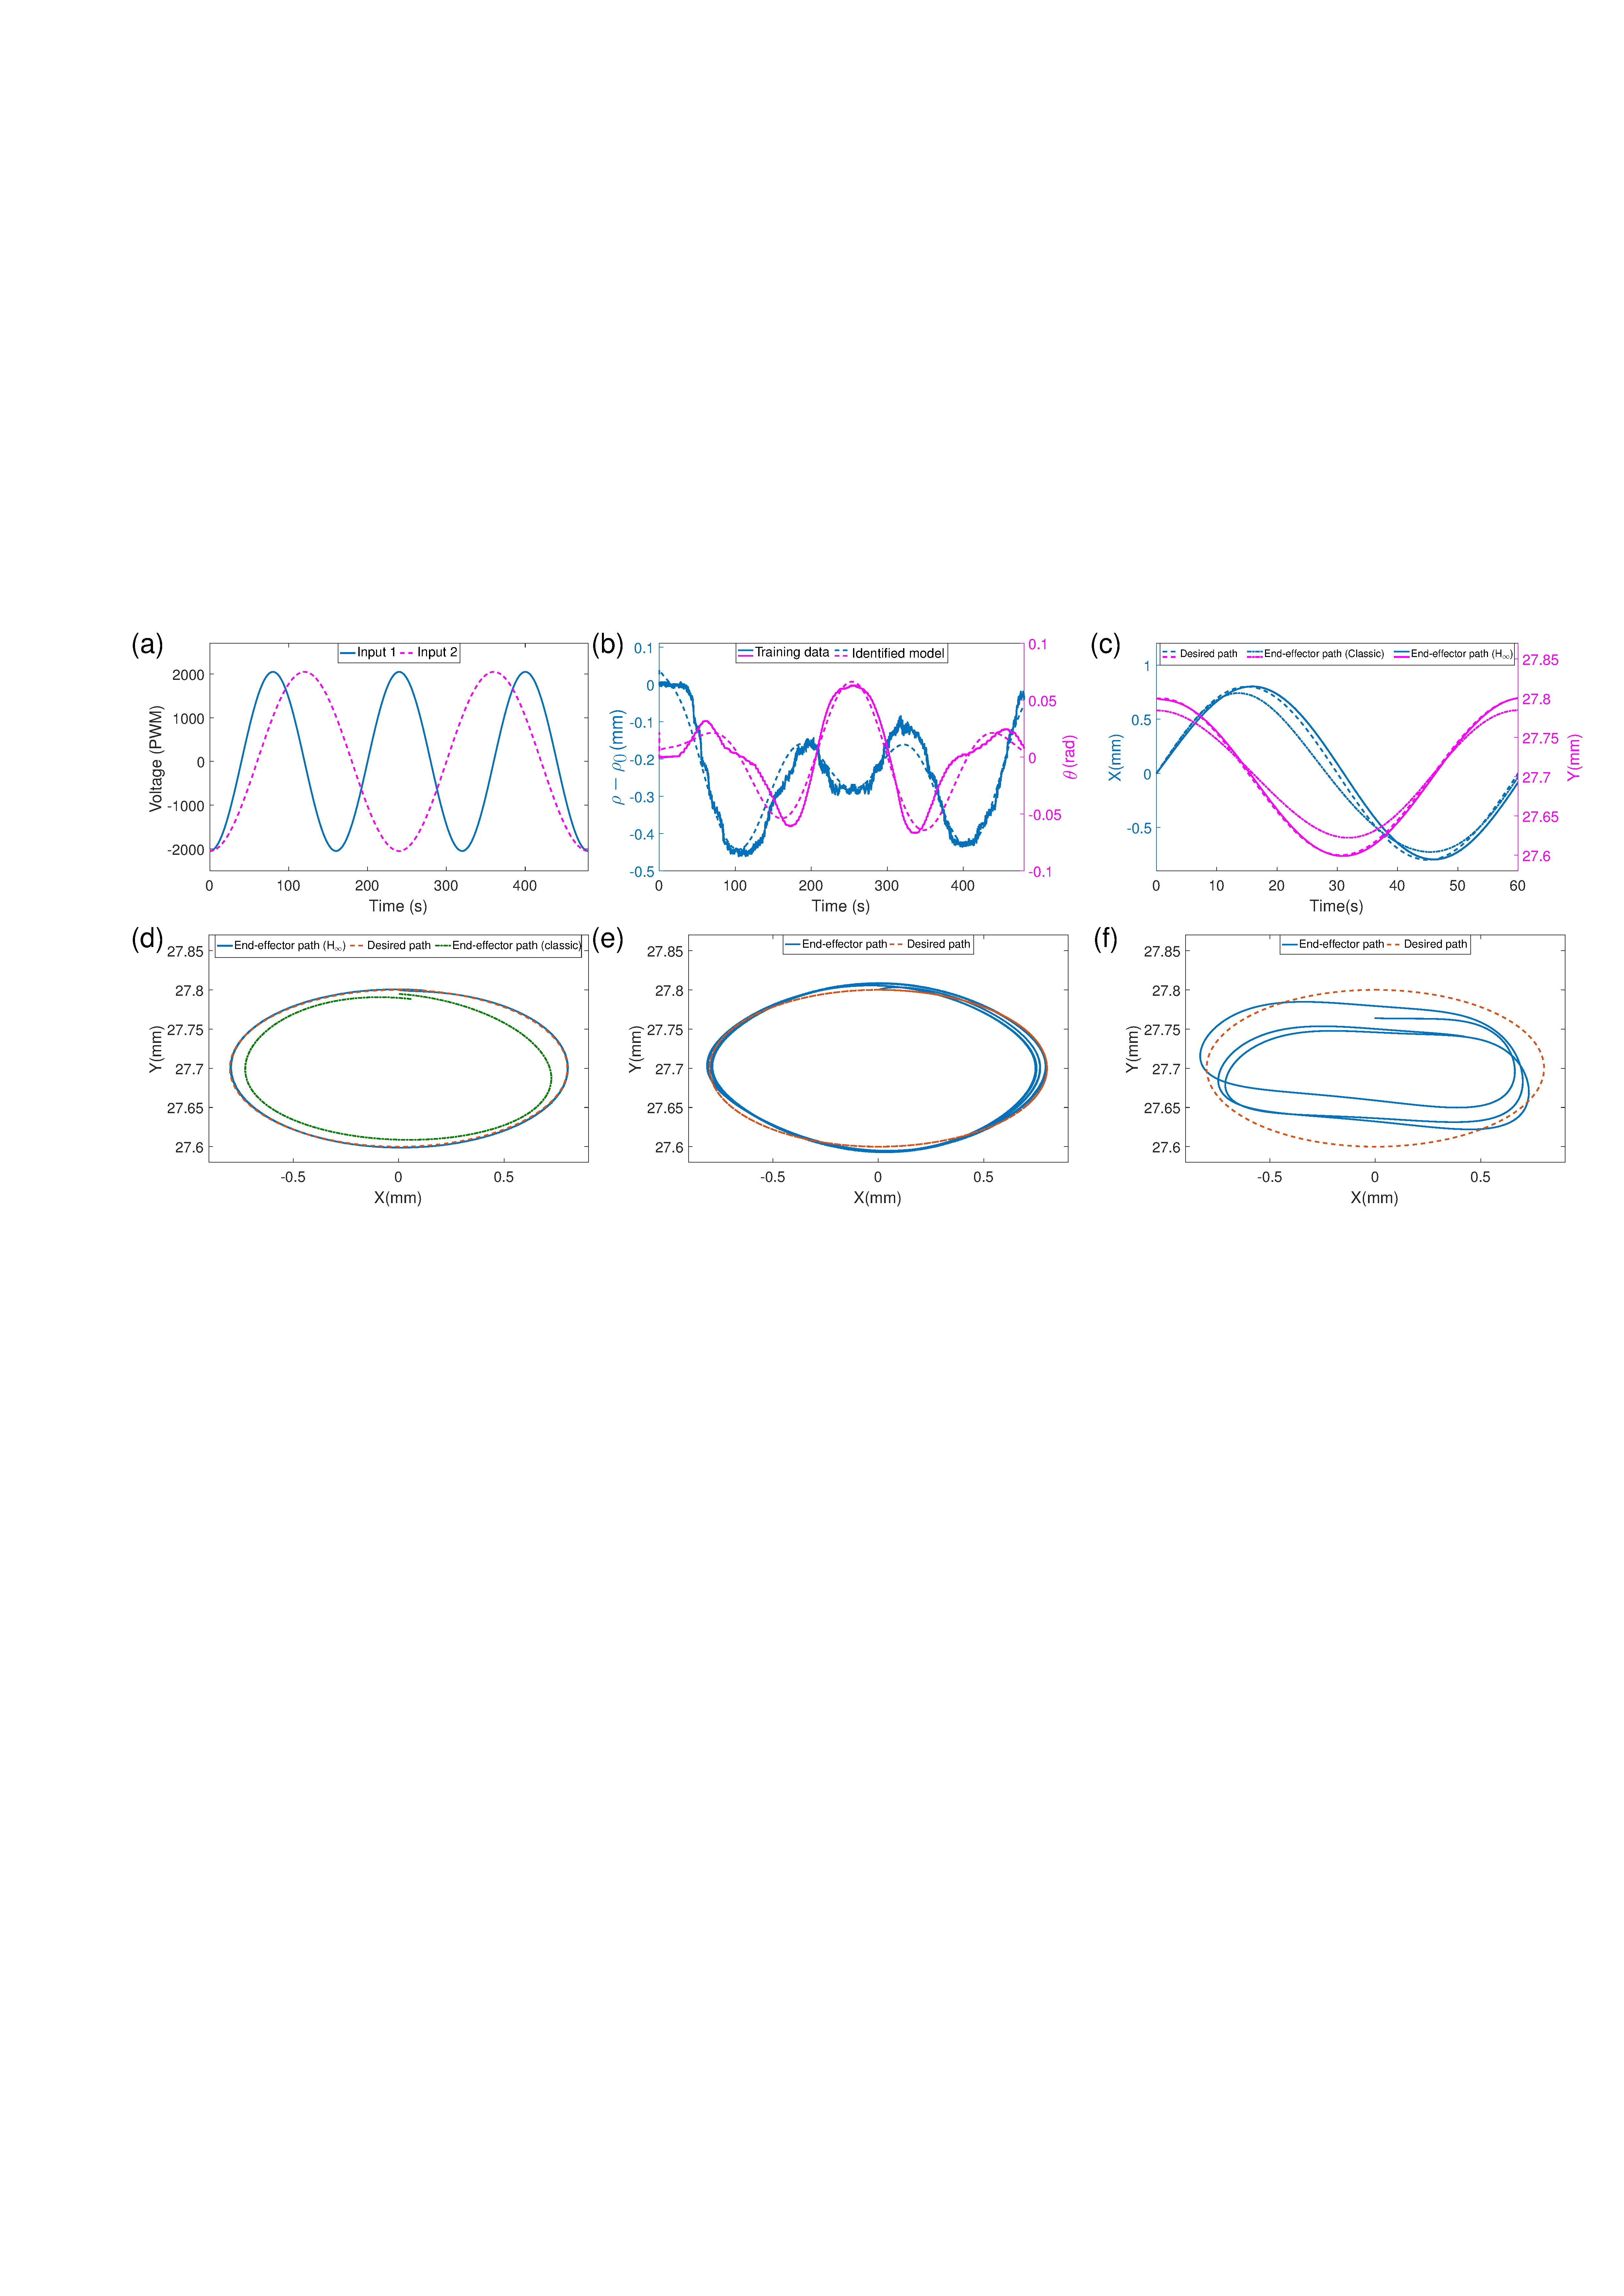
\includegraphics[width=\textwidth]{Figure_Sim_6.pdf}
    \caption[\capitalisewords{Simulation results of the controller}]{Simulation results. (a) 12-bit PWM waveform applied to the SVAs during training. (b) System output and model fitted from training. (c) The $x$ and $y$ coordinates of the manipulator tip over time for the $H_\infty$-optimal and Observer-based controllers, tracking an ellipse. (d) The $x$-$y$ trajectory of the tip during the simulation in (c).
    (e) $H_\infty$-optimal controller with noise and disturbance. (f) Observer-based controller with noise and disturbance.} \vspace{-0.5cm}
\label{fig:sim}
\end{figure*}

%--------------------------------------------------------
\section{\capitalisewords{Results and Discussion}}
% \dma{REVIEW WITH DMAs}

In this section, we study the performance of $H_\infty$ and observer controllers for trajectory tracking. An elliptical reference trajectory is used, defined by

\begin{align}
\vect{r}(t)= \begin{bmatrix} \alpha\sin\left(\frac{2\pi}{60}t\right) & \beta+\gamma\cos\left(\frac{2\pi}{60} t\right)
\end{bmatrix}^T. 
\end{align}
where $\alpha=0.8$, $\beta=27.7$, and $\gamma=0.1$ for the 25\,mm extension, and $\alpha=0.6$, $\beta=11.5$, and $\gamma=0.3$ for the 9\,mm extension, to ensure that each path lies in the workspace of its corresponding manipulator (see Fig.~\ref{fig:Path}). The manipulator's tracking performance degraded at frequencies of higher than one cycle per minute.% (Figs.~\ref{fig:Control_outputs}g and~\ref{fig:Control_outputs}h).

%\dma{REMOVE THIS:}
%The $H_\infty$-optimal controller is then implemented experimentally on the manipulator and evaluated for different reference trajectories and loads. Finally, we present an application of the $H_\infty$-optimal controller to payload transport by an array of four manipulators with 9\,mm extensions.

%--------------------------

\begin{table}[t]
\centering
\caption{N(MAE) of controller performance in simulation (in mm).}
\begin{tabular}{c c c c c c}
\hline
Controller&Noise $\&$& $x$ & $y$& $x-y$& $x-y$\\
           &disturbance& MAE & MAE & MAE & NMAE ($\%$)\\
\hline
% $H_{\infty}$       & 9\,mm & 0.044 & 0.017 & 0.055 & 4.1\\
% \rev{Observer}            & 9\,mm & 0.074 & 0.027 & 0.100 & 7.4\\
$H_{\infty}$       & No & 0.045 & 0.006 & 0.052 & 3.2\\
Observer            & No & 0.065 & 0.008 & 0.079 & 4.9\\
$H_{\infty}$ & Yes & 0.047 & 0.005 & 0.055 & 3.4\\
Observer & Yes & 0.078 & 0.009 & 0.096 & 5.9\\
\hline
\end{tabular}
\label{table:sim}
\vspace{-4mm}
\end{table}

\subsection{Comparison of controllers in simulation}
The performance of the two controllers is first compared in simulation in the presence of the following disturbance and noise signals:
\begin{align}
\vect{d}(t)&= \begin{bmatrix} 0.00015\sin\left(\frac{3\pi}{60}t\right) & 0.00045\sin\left(\frac{2\pi}{60} t\right)
\end{bmatrix}^T,\\
\vect{n}(t)&= \begin{bmatrix} 0.3\sin\left(\frac{\pi}{60}t\right) & 0.3\sin\left(\frac{0.5\pi}{60} t\right)
\end{bmatrix}^T. 
\end{align}
%To compare the performance of the observer-based and $H_{\infty}$-optimal controllers, 
The manipulator with the 25\,mm extension was simulated in MATLAB Simulink, using the output-feedback tracking framework depicted in Fig.~\ref{fig:control_block} and the identified model and controller values designed in the previous section.
Figures~\ref{fig:sim}c and~\ref{fig:sim}d plot the $x$ and $y$ coordinates and the trajectory of the manipulator tip over time for one cycle (60\,s), given an elliptical reference trajectory, from each controller. 
% A similar comparison was performed for a simulated manipulator with a 9\,mm extension,~(reported in Table~\ref{table:sim}). 
To observe the effect of adding noise and disturbance in simulation, the sinusoidal functions of $\vect{n}$ and $\vect{d}$ were input to the 25\,mm manipulator. The tracking trajectories of the manipulator tip produced by each controller are compared in Figs.~\ref{fig:sim}e and~\ref{fig:sim}f, separately. Although the simulations are performed across three cycles, only one cycle is shown in the figures and used in the error comparison for clarity. The tracking error for each case is reported in Table~\ref{table:sim}.The NMAE values were computed by dividing the mean absolute error (MAE) over their corresponding range. All the values are relatively low, under 10\%, indicating accurate tracking. 

%-------------------------------------------------------

%\begin{figure*}[t]
%\centering
    %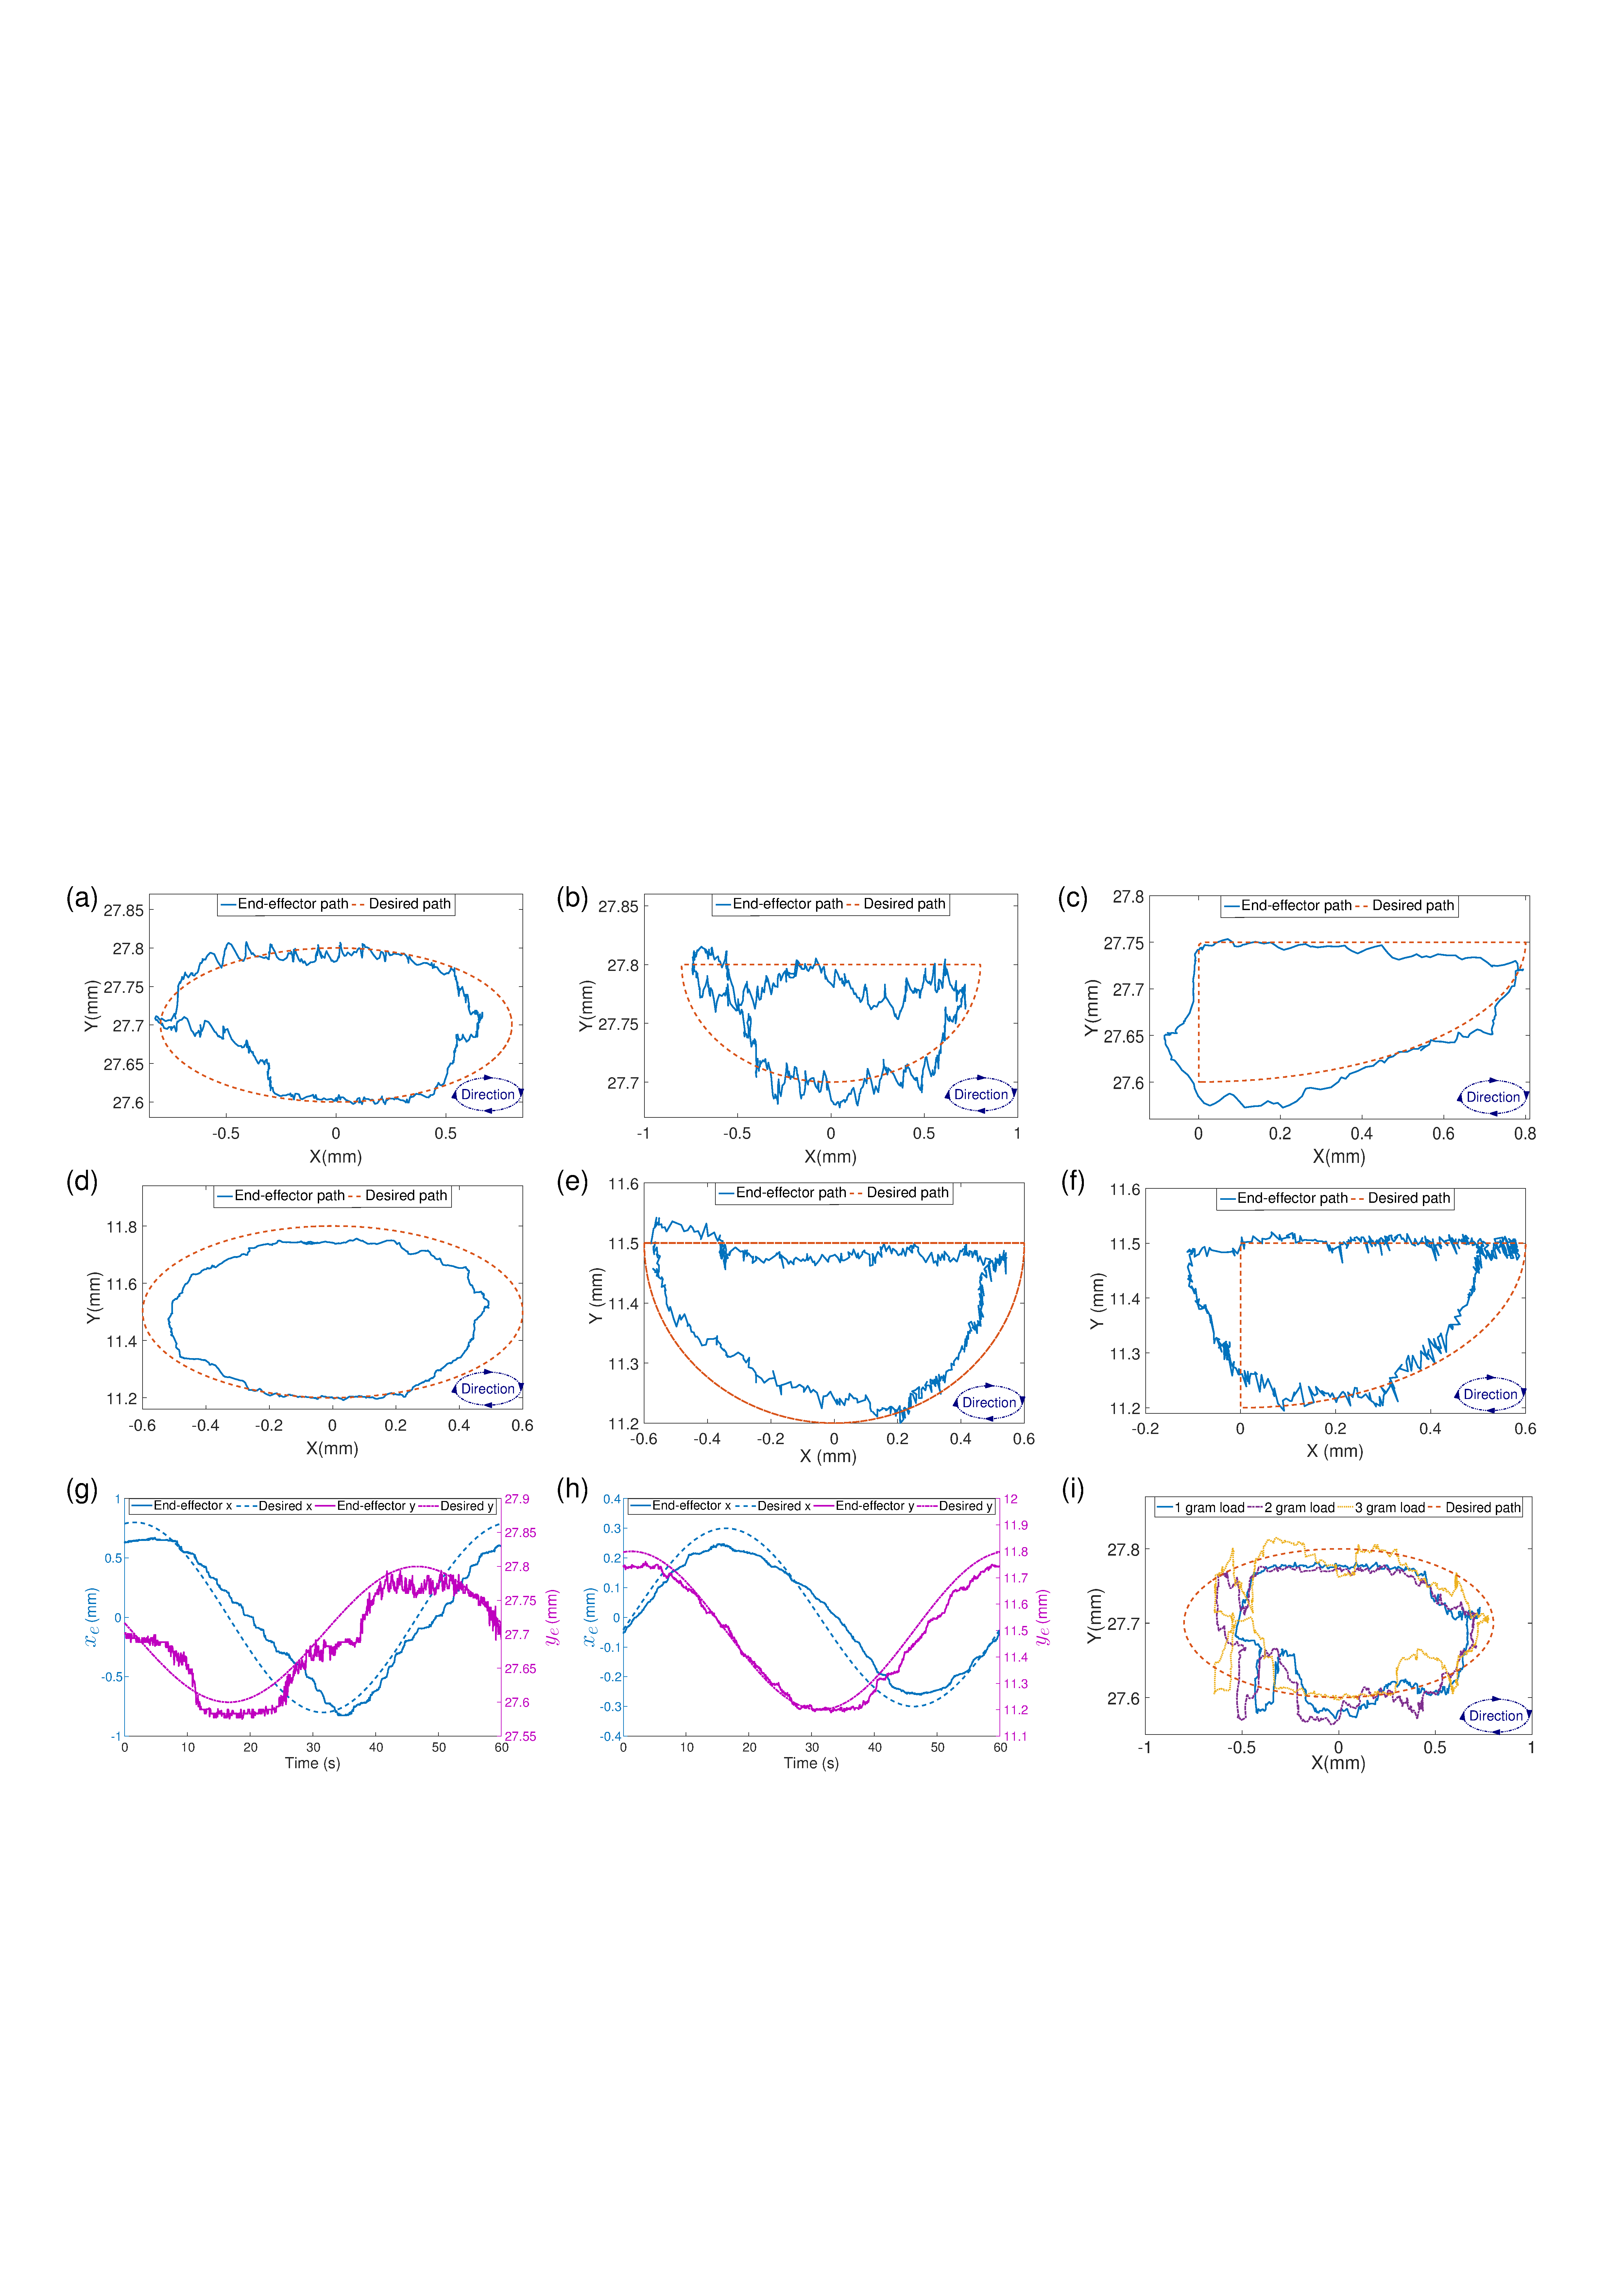
\includegraphics[width=\textwidth]{Control_Picture_New_Ten.pdf}
    %\caption[Tracking reference and experimental trajectories of  manipulator tip]{Tracking reference and experimental trajectories of  manipulator tip in Cartesian coordinates. 25\,mm manipulator tracking: (a) an elliptical trajectory; (b) a half-ellipse; (c) a quarter-ellipse. 9\,mm manipulator tracking: (d) an elliptical trajectory; (e) a half-ellipse; (f) a quarter-ellipse. (g) 25\,mm manipulator tracking an elliptical trajectory: $x,y$ coordinates over time separately. (h) 9\,mm manipulator tracking an elliptical trajectory: $x,y$ coordinates over time separately. (i) 25\,mm manipulator tracking an elliptical trajectory under 1\,g, 2\,g, and 3\,g.}
    %\label{fig:Control_outputs}
%\end{figure*}
%%--------------------------------------------------------------------
%\subsection{Experimental validation of $H_\infty$-optimal controller}
%
%Since the $H_\infty$-optimal controller exhibited higher tracking accuracy in simulation both with and without disturbance and noise, it was selected for experimental implementation. Using the designed control gain for $H_\infty$, we have implemented the output-feedback tracking framework depicted in Fig.~\ref{fig:control_block}b on the hydrogel-based manipulator (Fig.~\ref{fig:setup}). Half-ellipse and quarter-ellipse paths were also used as reference trajectories. Sources of noise in the experiment arise in the testing environment and vision-based feedback. Disturbances include modeling and manufacturing errors.  The MAE and NMAE values are reported for one cycle per trajectory in Table~\ref{table:control}, though three repeating cycles per trajectory were collected.
%
%Figure~\ref{fig:Control_outputs}a compares the trajectory of a manipulator with the 25\,mm extension driven by the controller Equation~\eqref{eq:Hinf-ctl} along an elliptical reference trajectory. Controller performance was evaluated using a half-ellipse and quarter-ellipse reference trajectory as well, to verify the ability of the controlled system to track straight lines and sharp turns (Figs.~\ref{fig:Control_outputs}b and~\ref{fig:Control_outputs}c). Figures~\ref{fig:Control_outputs}d, ~\ref{fig:Control_outputs}e ,and~\ref{fig:Control_outputs}f show the controlled position of the 9\,mm extension's tip using the same reference trajectories. Figures~\ref{fig:Control_outputs}g and~\ref{fig:Control_outputs}h illustrate the time evolution of the $x$ and $y$ coordinates separately for the two extensions.
%
%\begin{table}[t]
%\centering
%\caption{(N)MAE of $H_{\infty}$ controller performance in experiment.}\vspace{-0.25cm}
%\begin{tabular}{c c c c c c c}
%\hline
%\hspace{-2mm} $d$ & Reference & Load & $x$ & $y$ & $x-y$ & \hspace{-2mm} NMAE\\
%\hspace{-2mm} (mm) &  trajectory   & (g)  & (mm)& (mm)& (mm) & \hspace{-2mm}$\%$\\
%\hline
%\hspace{-2mm}25 & Ellipse          & - & 0.123 & 0.042 & 0.131 & \hspace{-2mm}8.1\\
%\hspace{-2mm}25 & Half Ellipse     & - & 0.119 & 0.023 & 0.123 & \hspace{-2mm}7.6\\
%\hspace{-2mm}25 & Quarter Ellipse  & - & 0.112 & 0.026 & 0.119 & \hspace{-2mm}7.4\\
%\hspace{-2mm}9 & Ellipse           & - & 0.088 & 0.033 & 0.099 & \hspace{-2mm}7.4\\
%\hspace{-2mm}9 & Half Ellipse      & - & 0.129 & 0.058 & 0.132 & \hspace{-2mm}9.8\\
%\hspace{-2mm}9 & Quarter Ellipse   & - & 0.161 & 0.061 & 0.171 & \hspace{-2mm}12.8\\
%\hspace{-2mm}25 & Ellipse          & 1 & 0.140 & 0.022 & 0.144 & \hspace{-2mm}8.9\\
%\hspace{-2mm}25 & Ellipse          & 2 & 0.162 & 0.021 & 0.162 & \hspace{-2mm}10.1\\
%\hspace{-2mm}25 & Ellipse          & 3 & 0.164 & 0.022 & 0.164 & \hspace{-2mm}10.2\\ 
%\hline
%\end{tabular}
%\label{table:control}
%\vspace{-4mm}
%\end{table}
%
%%-----------------------------------
%\begin{figure*}[t]
%\centering
%{\includegraphics[width=\textwidth]{Starfish_tube_feet_application_8.pdf}}
%\caption[Control of four 9\,mm manipulators in series for payload transport]{Control of four 9\,mm manipulators in series for payload transport, in a manner similar to food transport by starfish tube feet. (a) The manipulators, numbered 1 to 4 from left to right, are commanded to first follow the cyan dashed lines from their initial positions to their starting positions on the reference trajectories, and then follow these  trajectories, shown as red dashed lines. Manipulators 1 and 3 have a phase shift of $180^\circ$ compared to manipulators 2 and 4. (b) Illustration of a starfish-inspired robotic platform with four hydrogel-actuated manipulators. (c) Real starfish transporting a clam on its tube feet. (d) Displacement of the payload as a function of time for different reference trajectories and load weights. (e) Array of four manipulators functioning as described in (a) to transport the payload. Image was taken when the manipulators completed the first gait cycle. The payload is a clear flat acrylic plate with a black square on its left side. The positions of the manipulator tips are marked by triangles at their initial locations, circles at the start of the gait cycle, squares at the middle of the gait cycle, and diamonds at the end of the gait cycle.
%}
    %\label{fig:Control_payload}
%\end{figure*}
%In order to further characterize our system's actuation capabilities, the manipulator's trajectory-tracking performance under load was studied, as shown in Fig.~\ref{fig:Control_outputs}i. Loads (stainless steel nuts) weighing 1\,g, 2\,g, and 3\,g were placed on the 25\,mm extension, as shown in Fig.~\ref{fig:Path}b. The manipulator was commanded to follow the same elliptical trajectory as in the unloaded case. The results show that the addition of a weight of up to 3\,g increases the trajectory tracking NMAE from 8.1$\%$ to 10.2$\%$ (see Table~\ref{table:control}). Despite the increase in error, each actuator is still able to function under a load as large as 12.5 times its own weight (0.12\,g).
%% Tracking the given trajectories requires each SVA to cycle through multiple phases of heating and cooling. As can be observed in Fig.~\ref{fig:Control_outputs}, tracking error is evident for each reference trajectory.The largest tracking error in all cases occurs along a portion of the trajectory in the lower left quadrant of the plots, in which, both SVAs are cooling. Accounting for the different time-constants of the SVAs in heating and cooling states, this transition is not well-characterized in our model obtained by black-box system identification, which results in less accurate trajectory tracking along this portion. We believe, therefore, that the largest difference between our simulated and experimental results can be attributed to the model's inability to characterize the state of SVA heating or cooling. 
%As shown in Table~\ref{table:control}, the experimental NMAE values are higher than the simulation values, but remain below $15$\%.
%
%
%\subsection{Payload transport application} \label{sec:payload}
%Inspired by the way starfish transport food using their tube feet (Figs.~\ref{fig:Control_payload}b and~\ref{fig:Control_payload}c)~\cite{Kerkut1953,Pentreath1970}, we configured an array of four 9\,mm manipulators, as shown in Fig.~\ref{fig:Control_payload}e, and applied the proposed $H_\infty$-optimal controller in~\eqref{eq:Hinf-ctl} and Fig.~\ref{fig:control_block}b to each manipulator in order to transport a payload across their tips. The payload being transported is a clear acrylic plate. The manipulators are commanded to track reference trajectories as depicted in Fig.~\ref{fig:Control_payload}a, with phase shifts between adjacent manipulators. The payload moves to the right as the manipulators complete repeated cycles of the reference trajectories (``gait cycles''), as shown in Figs.~\ref{fig:Control_payload}d and~\ref{fig:Control_payload}e. The data from Fig.~\ref{fig:Control_payload}d on the duration of one gait cycle and the payload displacement in each tested scenario including the ones with extra added loads on the payload are reported in Table~\ref{table:table_Payload displacement}. A video of the payload transport is attached as supplementary material. The payload's position is recorded but not controlled in this exemplar application, since our goal in this chapter was to demonstrate a use-case for trajectory tracking control. However, many other platforms and applications are possible, including bio-inspired ones~\cite{Doroudchi2020}. Through this example, we have demonstrated how trajectory tracking control of systems with soft actuators, when applied to even simple platforms such as this 2-DOF manipulator, may be used to complete complex tasks such as object transport when used in parallel. This type of design can be used to simplify and decouple the control structures in future applications to reduce computational expense.
%
%\begin{table}[t]
%\centering
%\caption{Payload displacement $\Delta X$ with different reference trajectories for the manipulators.}
%\label{table:table_Payload displacement}
%\begin{tabular}{c c c c}
%
%% & & \\ 
%\hline
%Reference & Payload weight & Time for one & $\Delta X$ after five \\
%trajectory & + load (g) & gait cycle (s) & gait cycles (mm)\\
%\hline
%Ellipse         & 2.7   & 60  & 5.66\\
%Half-ellipse    & 2.7   & 50  & 4.55\\
%Quarter-ellipse & 2.7   & 40  & 7.10\\
%Ellipse         & 2.7+1 & 60  & 4.75\\
%Ellipse         & 2.7+2 & 60  & 4.84\\
%Ellipse         & 2.7+3 & 60  & 2.30\\
%% Open-loop  & 2.7~g & N/A & 2.04~mm\\
%\hline
%\end{tabular}
%\end{table}

%------------------------------------------------------
\subsection{prove that the ${H_{\infty}}$ gain is bounded}
%\appendix
We can prove that the ${H_{\infty}}$ gain is bounded using the bounded-real lemma~\cite{Boyd1994} below. 
% \vspace{1mm}

\textbf{Lemma}: \textit{Suppose that}
\begin{equation*}
\vect{G}(s)=\begin{bmatrix}
\begin{array}{c | c}
\vect{A}  &  \vect{B} \\
\hline
\vect{C}  & \vect{D}
\end{array}  
\end{bmatrix}.
\end{equation*}

\textit{Then, the following statements are equivalent:} 

1.~~$\norm{\vect{G}(s)}_{H_{\infty}}$ $\leq$ $\gamma$ \vspace{1mm}
    
2.~~There exists a $\vect{P} > 0$ such that 

    \begin{equation*}
		\begin{bmatrix}
		\vect{A}^T\vect{P}+\vect{PA} &  \vect{PB} \\
		\vect{B}^T\vect{P}    & -\gamma \vect{I} \\
		\end{bmatrix}+\dfrac{1}{\gamma}	\begin{bmatrix}
		\vect{C}^T\\
		\vect{D}^T\\
		\end{bmatrix}\begin{bmatrix}
		\vect{C} & \vect{D}\\
		\end{bmatrix} < 0
        %\vspace{-2mm}
		\label{eq-LMI}
		\end{equation*}

The proof that statement 1 implies 2 requires the Hamiltonian, and the proof that statement 2 implies 1 uses the global stability conditions of the Lyapunov function~\cite{Boyd1994}.
\section{\capitalisewords{Conclusion}}

In this chapter, we addressed a trajectory-tracking problem for a millimeter-scale 2-DOF manipulator with soft hydrogel-based actuators. We defined a linear state-space model of the manipulator and fit the matrices of this model using input-output measurement black-box identification. This state-space representation enables the implementation of a range of controllers on the manipulator; in this chapter, the performance of an observer-based controller was compared in simulation to that of an $H_{\infty}$-optimal controller in an output-feedback framework with and without noise and disturbance. We showed experimentally that different versions of the manipulator are able to track various reference trajectories, even under load, using the $H_{\infty}$-optimal controller.

Our ability to coordinate independently controllable soft actuators with complex internal dynamics in a robotic system demonstrates progress in the real-time, closed-loop control of mechanisms with this type of actuator. We expect that researchers will be able to adapt this approach across similar stimuli-responsive materials as they are developed and optimized. This will also permit SVAs, manufactured from a variety of materials, to be used for controlled grasping, manipulation, and locomotion tasks across a variety of new soft robotic platforms, such as octopus-inspired continuum robots~\cite{Doroudchi2020}. Our approach can be used to design and implement decentralized controllers on segmented mechanisms with distributed hydrogel actuators, as discussed in our related work~\cite{Doroudchi2020,Doroudchi2019}.

In future work, we plan to improve the speed of the image processing algorithms for tracking the manipulator, and ultimately eliminate the use of the camera for position tracking and instead implement this control scheme using embedded sensor feedback.  This will enable the application of machine learning techniques to optimize control performance.


\setcounter{chapter}{1}%
\setcounter{section}{1}%
\chapter{Curriculum Vitae}
\includepdf[pages=-,pagecommand={},width=1.3\textwidth]{CV.pdf}



%\addcontentsline{toc}{part}{BIOGRAPHICAL SKETCH}
%\biographicalpage{Enter content here.}
%\renewcommand{\chaptername}{CURRICULUM VITAE}
%\appendix
%\renewcommand{\chaptername}{APPENDIX}
%\addtocontents{toc}{APPENDIX \par}
%\appendix{b}


\end{document}